% To avoid execution of code, do opts_chunk$set(eval = FALSE)
% See options() calls below.  To force evaluation of all chunks, use
% the one with cache.rebuild = TRUE
\documentclass[12pt,oneside]{book}\usepackage[]{graphicx}\usepackage[]{color}
%% maxwidth is the original width if it is less than linewidth
%% otherwise use linewidth (to make sure the graphics do not exceed the margin)
\makeatletter
\def\maxwidth{ %
  \ifdim\Gin@nat@width>\linewidth
    \linewidth
  \else
    \Gin@nat@width
  \fi
}
\makeatother

\definecolor{fgcolor}{rgb}{0.345, 0.345, 0.345}
\newcommand{\hlnum}[1]{\textcolor[rgb]{0.686,0.059,0.569}{#1}}%
\newcommand{\hlstr}[1]{\textcolor[rgb]{0.192,0.494,0.8}{#1}}%
\newcommand{\hlcom}[1]{\textcolor[rgb]{0.678,0.584,0.686}{\textit{#1}}}%
\newcommand{\hlopt}[1]{\textcolor[rgb]{0,0,0}{#1}}%
\newcommand{\hlstd}[1]{\textcolor[rgb]{0.345,0.345,0.345}{#1}}%
\newcommand{\hlkwa}[1]{\textcolor[rgb]{0.161,0.373,0.58}{\textbf{#1}}}%
\newcommand{\hlkwb}[1]{\textcolor[rgb]{0.69,0.353,0.396}{#1}}%
\newcommand{\hlkwc}[1]{\textcolor[rgb]{0.333,0.667,0.333}{#1}}%
\newcommand{\hlkwd}[1]{\textcolor[rgb]{0.737,0.353,0.396}{\textbf{#1}}}%
\let\hlipl\hlkwb

\usepackage{framed}
\makeatletter
\newenvironment{kframe}{%
 \def\at@end@of@kframe{}%
 \ifinner\ifhmode%
  \def\at@end@of@kframe{\end{minipage}}%
  \begin{minipage}{\columnwidth}%
 \fi\fi%
 \def\FrameCommand##1{\hskip\@totalleftmargin \hskip-\fboxsep
 \colorbox{shadecolor}{##1}\hskip-\fboxsep
     % There is no \\@totalrightmargin, so:
     \hskip-\linewidth \hskip-\@totalleftmargin \hskip\columnwidth}%
 \MakeFramed {\advance\hsize-\width
   \@totalleftmargin\z@ \linewidth\hsize
   \@setminipage}}%
 {\par\unskip\endMakeFramed%
 \at@end@of@kframe}
\makeatother

\definecolor{shadecolor}{rgb}{.97, .97, .97}
\definecolor{messagecolor}{rgb}{0, 0, 0}
\definecolor{warningcolor}{rgb}{1, 0, 1}
\definecolor{errorcolor}{rgb}{1, 0, 0}
\newenvironment{knitrout}{}{} % an empty environment to be redefined in TeX

\usepackage{alltt}

\usepackage{bbding}
\usepackage[unicode=true]{hyperref}
\usepackage{multirow}
\usepackage{amsfonts}
\usepackage{amsmath}
\usepackage{geometry}
\usepackage{verbatim}
\usepackage{longtable}
\usepackage{enumitem}
\usepackage{color}
%\setlist{nosep}
\setlist{noitemsep}
\usepackage[numbers]{natbib}
\usepackage{multicol}

\geometry{tmargin = 1in, bmargin = 1in, lmargin = 1in, rmargin = 1in}

\def\file#1{\textsl{#1}}

\def\cd#1{\texttt{#1}}
\def\nm#1{\textit{#1}}
\newcommand{\ver}{0.6-5}

\hypersetup{colorlinks=true, linkcolor=red, urlcolor=blue}
\IfFileExists{upquote.sty}{\usepackage{upquote}}{}
\begin{document}
%\SweaveOpts{concordance=TRUE}
%\SweaveOpts{concordance=TRUE}
%\SweaveOpts{concordance=TRUE}




\title{NIMBLE User Manual}
\author{NIMBLE Development Team}
\date{Version \ver\\
  \vspace{3in}
\begin{figure}[!h]
  \begin{center}
  
\includegraphics[width=1.5in]{nimble-icon.png}
  \end{center}
\end{figure}
\href{http://R-nimble.org}
     {http://R-nimble.org} \\
\href{https://github.com/nimble-dev/nimble-docs/blob/master/UserManual}
     {https://github.com/nimble-dev/nimble-docs}
}
\maketitle
% load these prior to building the manual, because otherwise they
% generate package loading messages that I don't know how to stop.


\begingroup
\hypersetup{linkcolor=blue}
%\hypersetup{linkcolor=green,pdfborderstyle={/S/U/W 1}}
\tableofcontents
\endgroup

\part{Introduction}
\label{part:models}


%% See http://yihui.name/knitr/demo/child/ for documentation on the parent/child document system of knitr



\chapter{Welcome to NIMBLE}
\label{sec:welcome-nimble}

NIMBLE is a system for building and sharing analysis methods for
statistical models from R, especially for hierarchical models and
computationally-intensive methods.  While NIMBLE is embedded in R, it
goes beyond R by supporting separate programming of models and
algorithms along with compilation for fast execution.  

As of version \ver, NIMBLE has been around for a while and is reasonably
stable, but we have a lot of plans to expand and improve it.  The
algorithm library provides MCMC with a lot of user control and ability
to write new samplers easily.  Other algorithms include particle
filtering (sequential Monte Carlo) and Monte Carlo Expectation
Maximization (MCEM).  

But NIMBLE is about much more than providing an algorithm library.  It
provides a language for writing model-generic algorithms.  We hope you
will program in NIMBLE and make an R package providing your method.
Of course, NIMBLE is open source, so we also hope you'll contribute to
its development.

Please join the mailing lists
(see \href{https://r-nimble.org/more/issues-and-groups}{R-nimble.org/more/issues-and-groups}) and help improve NIMBLE by
telling us what you want to do with it, what you like, and what could
be better.  We have a lot of ideas for how to improve it, but we want
your help and ideas too.  You can also follow and contribute to
developer discussions on the
\href{https://github.com/nimble-dev/nimble/wiki}{wiki of our GitHub
  repository}.

\section{What does NIMBLE do?}
\label{sec:what-is-nimble}

NIMBLE makes it easier to program statistical algorithms that will run
efficiently and work on many different models from R.

You can think of NIMBLE as comprising four pieces:

\begin{enumerate}
\item A system for writing statistical models flexibly, which is an
  extension of the BUGS language\footnote{See Chapter
    \ref{cha:writing-models} for information about NIMBLE's version of
    BUGS.}.
\item A library of algorithms such as MCMC.
\item A language, called NIMBLE, embedded within and similar in style
  to R, for writing algorithms that operate on models written in BUGS.
\item  A compiler that generates C++ for your models and algorithms,
  compiles that C++, and lets you use it seamlessly from R without
  knowing anything about C++.
\end{enumerate}

NIMBLE stands for Numerical Inference for statistical Models for
Bayesian and Likelihood Estimation.  

Although NIMBLE was motivated by algorithms for hierarchical
statistical models, it's useful for other goals too.  You could use it
for simpler models.  And since NIMBLE can automatically compile R-like
functions into C++ that use the Eigen library for fast linear algebra,
you can use it to program fast numerical functions without any model
involved\footnote{The packages \href{http://www.rcpp.org/}{Rcpp} and
  RcppEigen provide different ways of connecting C++, the Eigen
  library and R.  In those packages you program directly in C++, while
  in NIMBLE you program in R in a nimbleFunction and the NIMBLE compiler
  turns it into C++.}

One of the beauties of R is that many of the high-level analysis
functions are themselves written in R, so it is easy to see their code and modify
them.  The same is true for NIMBLE: the algorithms are themselves
written in the NIMBLE language.

\section{How to use this manual}

We suggest everyone start with the Lightning Introduction in Chapter \ref{cha:intro}.

Then, if you want to jump into using NIMBLE's algorithms without learning
about NIMBLE's programming system, go to Part \ref{part:models} to
learn how to build your model and Part \ref{part:algorithms} to learn
how to apply NIMBLE's built-in algorithms to your model.

If you want to learn about NIMBLE programming (nimbleFunctions), go to Part
\ref{part:programming}. This teaches how to program user-defined
function or distributions to use in BUGS code, compile your R code for
faster operations, and write algorithms with NIMBLE. These algorithms
could be specific algorithms for your particular model (such as a
user-defined MCMC sampler for a parameter in your model) or general
algorithms you can distribute to others. In fact the algorithms
provided as part of NIMBLE and described in Part \ref{part:algorithms}
are written as nimbleFunctions.


%% See http://yihui.name/knitr/demo/child/ for documentation on the parent/child document system of knitr







\chapter{Lightning introduction}
\label{cha:intro}

\section{A brief example}
\label{sec:brief-example}

Here we'll give a simple example of building a model and running some algorithms on the model, as well as creating our own user-specified algorithm. The goal is to give you a sense for what one can do in the system. Later sections will provide more detail.

We'll use the \nm{pump} model example from BUGS\footnote{The data set
  describes failure rates of some pumps.}.  We could load the model
from the standard BUGS example file formats (Section \ref{sec:readBUGSmodel}), but instead we'll show
how to enter it directly in R.

In this ``lightning introduction'' we will:

\begin{enumerate}
\item Create the model for the pump example.
\item Compile the model.
\item Create a basic MCMC configuration for the pump model.
\item Compile and run the MCMC
\item Customize the MCMC configuration and compile and run that.
\item Create, compile and run a Monte Carlo Expectation Maximization (MCEM)
  algorithm, which illustrates some of the flexibility NIMBLE
  provides to combine R and NIMBLE.
\item Write a short \cd{nimbleFunction} to generate simulations from
  designated nodes of any  model.
\end{enumerate}


\section{Creating a model}
\label{sec:creating-model}
First we define the model code, its constants, data, and initial
values for MCMC.

\begin{knitrout}
\definecolor{shadecolor}{rgb}{0.969, 0.969, 0.969}\color{fgcolor}\begin{kframe}
\begin{alltt}
\hlstd{pumpCode} \hlkwb{<-} \hlkwd{nimbleCode}\hlstd{(\{}
  \hlkwa{for} \hlstd{(i} \hlkwa{in} \hlnum{1}\hlopt{:}\hlstd{N)\{}
      \hlstd{theta[i]} \hlopt{~} \hlkwd{dgamma}\hlstd{(alpha,beta)}
      \hlstd{lambda[i]} \hlkwb{<-} \hlstd{theta[i]}\hlopt{*}\hlstd{t[i]}
      \hlstd{x[i]} \hlopt{~} \hlkwd{dpois}\hlstd{(lambda[i])}
  \hlstd{\}}
  \hlstd{alpha} \hlopt{~} \hlkwd{dexp}\hlstd{(}\hlnum{1.0}\hlstd{)}
  \hlstd{beta} \hlopt{~} \hlkwd{dgamma}\hlstd{(}\hlnum{0.1}\hlstd{,}\hlnum{1.0}\hlstd{)}
\hlstd{\})}

\hlstd{pumpConsts} \hlkwb{<-} \hlkwd{list}\hlstd{(}\hlkwc{N} \hlstd{=} \hlnum{10}\hlstd{,}
                   \hlkwc{t} \hlstd{=} \hlkwd{c}\hlstd{(}\hlnum{94.3}\hlstd{,} \hlnum{15.7}\hlstd{,} \hlnum{62.9}\hlstd{,} \hlnum{126}\hlstd{,} \hlnum{5.24}\hlstd{,}
                       \hlnum{31.4}\hlstd{,} \hlnum{1.05}\hlstd{,} \hlnum{1.05}\hlstd{,} \hlnum{2.1}\hlstd{,} \hlnum{10.5}\hlstd{))}

\hlstd{pumpData} \hlkwb{<-} \hlkwd{list}\hlstd{(}\hlkwc{x} \hlstd{=} \hlkwd{c}\hlstd{(}\hlnum{5}\hlstd{,} \hlnum{1}\hlstd{,} \hlnum{5}\hlstd{,} \hlnum{14}\hlstd{,} \hlnum{3}\hlstd{,} \hlnum{19}\hlstd{,} \hlnum{1}\hlstd{,} \hlnum{1}\hlstd{,} \hlnum{4}\hlstd{,} \hlnum{22}\hlstd{))}

\hlstd{pumpInits} \hlkwb{<-} \hlkwd{list}\hlstd{(}\hlkwc{alpha} \hlstd{=} \hlnum{1}\hlstd{,} \hlkwc{beta} \hlstd{=} \hlnum{1}\hlstd{,}
                  \hlkwc{theta} \hlstd{=} \hlkwd{rep}\hlstd{(}\hlnum{0.1}\hlstd{, pumpConsts}\hlopt{$}\hlstd{N))}
\end{alltt}
\end{kframe}
\end{knitrout}

Here \cd{x[i]} is the number of failures recorded during a time
duration of length \cd{t[i]} for the \cd{i}$^{th}$ pump.
\cd{theta[i]} is a failure rate, and the goal is estimate parameters
\cd{alpha} and \cd{beta}.  Now let's create the model and look at some of its nodes.

\begin{knitrout}
\definecolor{shadecolor}{rgb}{0.969, 0.969, 0.969}\color{fgcolor}\begin{kframe}
\begin{alltt}
\hlstd{pump} \hlkwb{<-} \hlkwd{nimbleModel}\hlstd{(}\hlkwc{code} \hlstd{= pumpCode,} \hlkwc{name} \hlstd{=} \hlstr{"pump"}\hlstd{,} \hlkwc{constants} \hlstd{= pumpConsts,}
                    \hlkwc{data} \hlstd{= pumpData,} \hlkwc{inits} \hlstd{= pumpInits)}

\hlstd{pump}\hlopt{$}\hlkwd{getNodeNames}\hlstd{()}
\end{alltt}
\begin{verbatim}
##  [1] "alpha"               "beta"               
##  [3] "lifted_d1_over_beta" "theta[1]"           
##  [5] "theta[2]"            "theta[3]"           
##  [7] "theta[4]"            "theta[5]"           
##  [9] "theta[6]"            "theta[7]"           
## [11] "theta[8]"            "theta[9]"           
## [13] "theta[10]"           "lambda[1]"          
## [15] "lambda[2]"           "lambda[3]"          
## [17] "lambda[4]"           "lambda[5]"          
## [19] "lambda[6]"           "lambda[7]"          
## [21] "lambda[8]"           "lambda[9]"          
## [23] "lambda[10]"          "x[1]"               
## [25] "x[2]"                "x[3]"               
## [27] "x[4]"                "x[5]"               
## [29] "x[6]"                "x[7]"               
## [31] "x[8]"                "x[9]"               
## [33] "x[10]"
\end{verbatim}
\begin{alltt}
\hlstd{pump}\hlopt{$}\hlstd{x}
\end{alltt}
\begin{verbatim}
##  [1]  5  1  5 14  3 19  1  1  4 22
\end{verbatim}
\begin{alltt}
\hlstd{pump}\hlopt{$}\hlstd{logProb_x}
\end{alltt}
\begin{verbatim}
##  [1]  -2.998011  -1.118924  -1.882686  -2.319466  -4.254550
##  [6] -20.739651  -2.358795  -2.358795  -9.630645 -48.447798
\end{verbatim}
\begin{alltt}
\hlstd{pump}\hlopt{$}\hlstd{alpha}
\end{alltt}
\begin{verbatim}
## [1] 1
\end{verbatim}
\begin{alltt}
\hlstd{pump}\hlopt{$}\hlstd{theta}
\end{alltt}
\begin{verbatim}
##  [1] 0.1 0.1 0.1 0.1 0.1 0.1 0.1 0.1 0.1 0.1
\end{verbatim}
\begin{alltt}
\hlstd{pump}\hlopt{$}\hlstd{lambda}
\end{alltt}
\begin{verbatim}
##  [1]  9.430  1.570  6.290 12.600  0.524  3.140  0.105  0.105
##  [9]  0.210  1.050
\end{verbatim}
\end{kframe}
\end{knitrout}


Notice that in the list of nodes, NIMBLE has introduced a new node,
\cd{lifted\_d1\_over\_beta}. We call this a ``lifted'' node. Like R,
NIMBLE allows alternative parameterizations, such as the scale or rate
parameterization of the gamma distribution. Choice of parameterization
can generate a lifted node, as can using a link function or a
distribution argument that is an expression. It's helpful to know why
they exist, but you shouldn't need to worry about them.

Thanks to the plotting capabilities of the \cd{igraph} package that
NIMBLE uses to represent the directed acyclic graph, we can plot the
model  (Figure 2.1).

\begin{knitrout}
\definecolor{shadecolor}{rgb}{0.969, 0.969, 0.969}\color{fgcolor}\begin{kframe}
\begin{alltt}
\hlstd{pump}\hlopt{$}\hlkwd{plotGraph}\hlstd{()}
\end{alltt}
\end{kframe}\begin{figure}
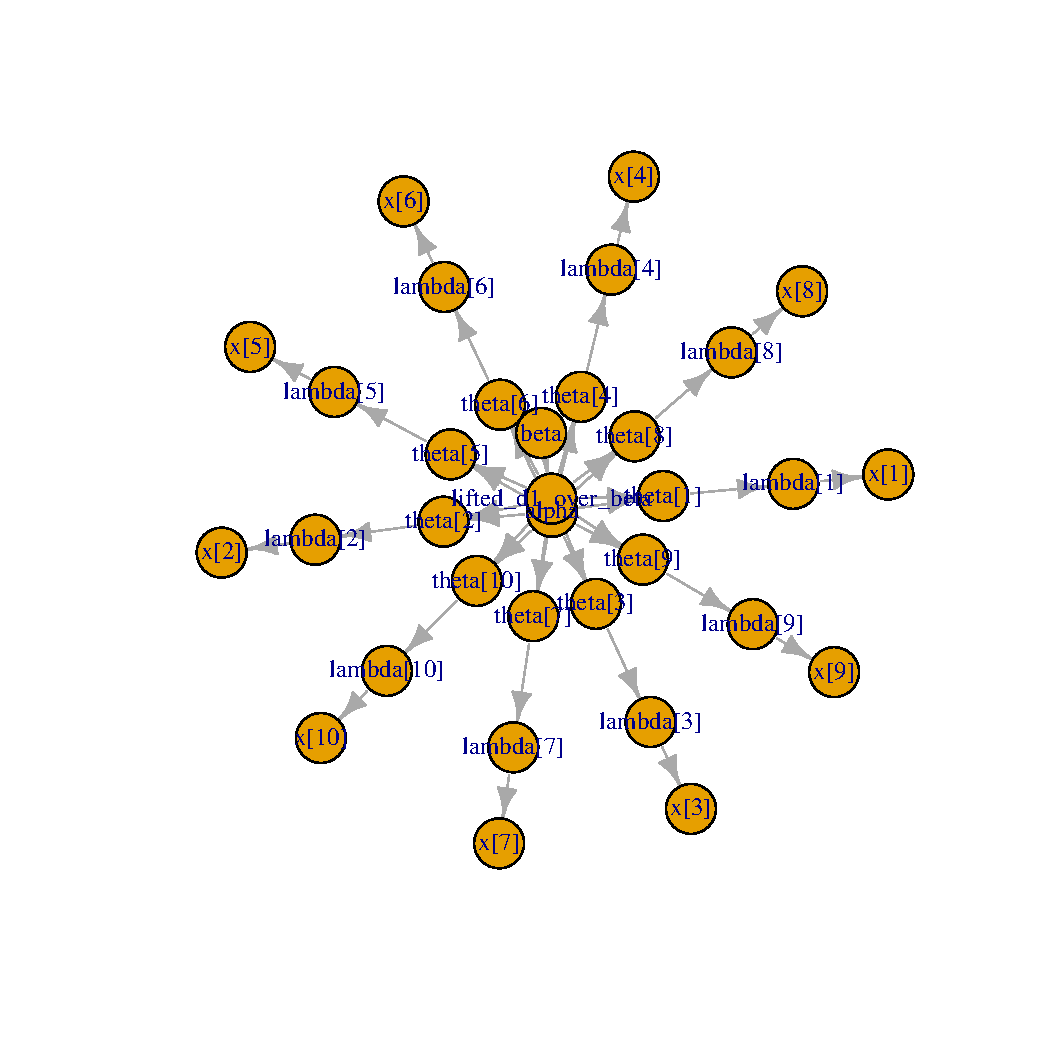
\includegraphics[width=\maxwidth]{figure/plotPump-1} \caption[Directed Acyclic Graph plot of the pump model, thanks to the igraph package]{Directed Acyclic Graph plot of the pump model, thanks to the igraph package}\label{fig:plotPump}
\end{figure}


\end{knitrout}

You are in control of the model.  By default, \cd{nimbleModel} does
its best to initialize a model, but let's say you want to
re-initialize \cd{theta}.  To simulate from the prior for \cd{theta} (overwriting the
initial values previously in the model) we first need to be sure the
parent nodes of all \cd{theta[i]} nodes are fully initialized, including any non-stochastic nodes such
as lifted nodes.  We then use the \cd{simulate} function to simulate
from the distribution for \cd{theta}.  Finally we use the
\cd{calculate} function to 
calculate the dependencies of \cd{theta}, namely \cd{lambda} and the
log probabilities of \cd{x} to ensure all parts of the
model are up to date.  First we show how
to use the model's \cd{getDependencies} method to query information
about its graph.

% TODO: the logic here is a bit weird - we say we want to know all parents of theta are initialized by our code actually finds dependencies of alpha+beta not parents of theta

\begin{knitrout}
\definecolor{shadecolor}{rgb}{0.969, 0.969, 0.969}\color{fgcolor}\begin{kframe}
\begin{alltt}
\hlcom{## Show all dependencies of alpha and beta terminating in stochastic nodes}
\hlstd{pump}\hlopt{$}\hlkwd{getDependencies}\hlstd{(}\hlkwd{c}\hlstd{(}\hlstr{"alpha"}\hlstd{,} \hlstr{"beta"}\hlstd{))}
\end{alltt}
\begin{verbatim}
##  [1] "alpha"               "beta"               
##  [3] "lifted_d1_over_beta" "theta[1]"           
##  [5] "theta[2]"            "theta[3]"           
##  [7] "theta[4]"            "theta[5]"           
##  [9] "theta[6]"            "theta[7]"           
## [11] "theta[8]"            "theta[9]"           
## [13] "theta[10]"
\end{verbatim}
\begin{alltt}
\hlcom{## Now show only the deterministic dependencies}
\hlstd{pump}\hlopt{$}\hlkwd{getDependencies}\hlstd{(}\hlkwd{c}\hlstd{(}\hlstr{"alpha"}\hlstd{,} \hlstr{"beta"}\hlstd{),} \hlkwc{determOnly} \hlstd{=} \hlnum{TRUE}\hlstd{)}
\end{alltt}
\begin{verbatim}
## [1] "lifted_d1_over_beta"
\end{verbatim}
\begin{alltt}
\hlcom{## Check that the lifted node was initialized. }
\hlstd{pump[[}\hlstr{"lifted_d1_over_beta"}\hlstd{]]} \hlcom{## It was.}
\end{alltt}
\begin{verbatim}
## [1] 1
\end{verbatim}
\begin{alltt}
\hlcom{## Now let's simulate new theta values}
\hlkwd{set.seed}\hlstd{(}\hlnum{1}\hlstd{)} \hlcom{## This makes the simulations here reproducible}
\hlstd{pump}\hlopt{$}\hlkwd{simulate}\hlstd{(}\hlstr{"theta"}\hlstd{)}
\hlstd{pump}\hlopt{$}\hlstd{theta}   \hlcom{## the new theta values}
\end{alltt}
\begin{verbatim}
##  [1] 0.15514136 1.88240160 1.80451250 0.83617765 1.22254365
##  [6] 1.15835525 0.99001994 0.30737332 0.09461909 0.15720154
\end{verbatim}
\begin{alltt}
\hlcom{## lambda and logProb_x haven't been re-calculated yet}
\hlstd{pump}\hlopt{$}\hlstd{lambda} \hlcom{## these are the same values as above}
\end{alltt}
\begin{verbatim}
##  [1]  9.430  1.570  6.290 12.600  0.524  3.140  0.105  0.105
##  [9]  0.210  1.050
\end{verbatim}
\begin{alltt}
\hlstd{pump}\hlopt{$}\hlstd{logProb_x}
\end{alltt}
\begin{verbatim}
##  [1]  -2.998011  -1.118924  -1.882686  -2.319466  -4.254550
##  [6] -20.739651  -2.358795  -2.358795  -9.630645 -48.447798
\end{verbatim}
\begin{alltt}
\hlstd{pump}\hlopt{$}\hlkwd{getLogProb}\hlstd{(}\hlstr{"x"}\hlstd{)} \hlcom{## The sum of logProb_x}
\end{alltt}
\begin{verbatim}
## [1] -96.10932
\end{verbatim}
\begin{alltt}
\hlstd{pump}\hlopt{$}\hlkwd{calculate}\hlstd{(pump}\hlopt{$}\hlkwd{getDependencies}\hlstd{(}\hlkwd{c}\hlstd{(}\hlstr{"theta"}\hlstd{)))}
\end{alltt}
\begin{verbatim}
## [1] -262.204
\end{verbatim}
\begin{alltt}
\hlstd{pump}\hlopt{$}\hlstd{lambda}  \hlcom{## Now they have.}
\end{alltt}
\begin{verbatim}
##  [1]  14.6298299  29.5537051 113.5038360 105.3583839   6.4061287
##  [6]  36.3723548   1.0395209   0.3227420   0.1987001   1.6506161
\end{verbatim}
\begin{alltt}
\hlstd{pump}\hlopt{$}\hlstd{logProb_x}
\end{alltt}
\begin{verbatim}
##  [1]  -6.002009 -26.167496 -94.632145 -65.346457  -2.626123
##  [6]  -7.429868  -1.000761  -1.453644  -9.840589 -39.096527
\end{verbatim}
\end{kframe}
\end{knitrout}

Notice that the first \cd{getDependencies} call returned dependencies
from \cd{alpha} and \cd{beta} down to the next stochastic nodes in the
model.  The second call requested only deterministic dependencies.
The call to \cd{pump\$simulate("theta")}
expands \cd{"theta"} to include all nodes in \cd{theta}.  After
simulating into \cd{theta}, we can see that \cd{lambda} and the log
probabilities of \cd{x} still reflect the old values of \cd{theta}, so
we \cd{calculate} them and then see that they have been updated.

\section{Compiling the model}
\label{sec:compiling-model}

Next we compile the model, which means generating C++ code, compiling
that code, and loading it back into R with an object that can be used just
like the uncompiled model. The values in the compiled model will be
initialized from those of the original model in R, but
the original and compiled models are distinct objects so any
subsequent changes in one will not be reflected in the other.

\begin{knitrout}
\definecolor{shadecolor}{rgb}{0.969, 0.969, 0.969}\color{fgcolor}\begin{kframe}
\begin{alltt}
\hlstd{Cpump} \hlkwb{<-} \hlkwd{compileNimble}\hlstd{(pump)}
\hlstd{Cpump}\hlopt{$}\hlstd{theta}
\end{alltt}
\begin{verbatim}
##  [1] 0.15514136 1.88240160 1.80451250 0.83617765 1.22254365
##  [6] 1.15835525 0.99001994 0.30737332 0.09461909 0.15720154
\end{verbatim}
\end{kframe}
\end{knitrout}

Note that the compiled model is used when running any NIMBLE algorithms via C++, so the model needs to be compiled before (or at the same time as) any compilation of algorithms, such as the compilation of the MCMC done in the next section.

\section{Creating, compiling and running a basic MCMC configuration}
\label{sec:creating-mcmc}
  
At this point we have initial values for all of the nodes in the model,
and we have both the original and compiled versions of the model. As a first algorithm
to try on our model, let's use NIMBLE's default MCMC. Note that conjugate relationships are detected for all nodes except for
\cd{alpha}, on which the default sampler is a random walk Metropolis sampler.
%\footnote{We haven't set up conjugate relationships for an
%  exponential yet.}
% footnote is true but not relevant as there is not a conj relationship for alpha in a gamma-distributed dependency

\begin{knitrout}
\definecolor{shadecolor}{rgb}{0.969, 0.969, 0.969}\color{fgcolor}\begin{kframe}
\begin{alltt}
\hlstd{pumpConf} \hlkwb{<-} \hlkwd{configureMCMC}\hlstd{(pump,} \hlkwc{print} \hlstd{=} \hlnum{TRUE}\hlstd{)}
\end{alltt}
\begin{verbatim}
## [1]  RW sampler: alpha
## [2]  conjugate_dgamma_dgamma sampler: beta
## [3]  conjugate_dgamma_dpois sampler: theta[1]
## [4]  conjugate_dgamma_dpois sampler: theta[2]
## [5]  conjugate_dgamma_dpois sampler: theta[3]
## [6]  conjugate_dgamma_dpois sampler: theta[4]
## [7]  conjugate_dgamma_dpois sampler: theta[5]
## [8]  conjugate_dgamma_dpois sampler: theta[6]
## [9]  conjugate_dgamma_dpois sampler: theta[7]
## [10] conjugate_dgamma_dpois sampler: theta[8]
## [11] conjugate_dgamma_dpois sampler: theta[9]
## [12] conjugate_dgamma_dpois sampler: theta[10]
\end{verbatim}
\begin{alltt}
\hlstd{pumpConf}\hlopt{$}\hlkwd{addMonitors}\hlstd{(}\hlkwd{c}\hlstd{(}\hlstr{"alpha"}\hlstd{,} \hlstr{"beta"}\hlstd{,} \hlstr{"theta"}\hlstd{))}
\end{alltt}
\begin{verbatim}
## thin = 1: alpha, beta, theta
\end{verbatim}
\begin{alltt}
\hlstd{pumpMCMC} \hlkwb{<-} \hlkwd{buildMCMC}\hlstd{(pumpConf)}
\hlstd{CpumpMCMC} \hlkwb{<-} \hlkwd{compileNimble}\hlstd{(pumpMCMC,} \hlkwc{project} \hlstd{= pump)}

\hlstd{niter} \hlkwb{<-} \hlnum{1000}
\hlkwd{set.seed}\hlstd{(}\hlnum{1}\hlstd{)}
\hlstd{CpumpMCMC}\hlopt{$}\hlkwd{run}\hlstd{(niter)}
\end{alltt}
\begin{verbatim}
## NULL
\end{verbatim}
\begin{alltt}
\hlstd{samples} \hlkwb{<-} \hlkwd{as.matrix}\hlstd{(CpumpMCMC}\hlopt{$}\hlstd{mvSamples)}

\hlkwd{par}\hlstd{(}\hlkwc{mfrow} \hlstd{=} \hlkwd{c}\hlstd{(}\hlnum{1}\hlstd{,} \hlnum{4}\hlstd{),} \hlkwc{mai} \hlstd{=} \hlkwd{c}\hlstd{(}\hlnum{.6}\hlstd{,} \hlnum{.4}\hlstd{,} \hlnum{.1}\hlstd{,} \hlnum{.2}\hlstd{))}
\hlkwd{plot}\hlstd{(samples[ ,} \hlstr{"alpha"}\hlstd{],} \hlkwc{type} \hlstd{=} \hlstr{"l"}\hlstd{,} \hlkwc{xlab} \hlstd{=} \hlstr{"iteration"}\hlstd{,}
     \hlkwc{ylab} \hlstd{=} \hlkwd{expression}\hlstd{(alpha))}
\hlkwd{plot}\hlstd{(samples[ ,} \hlstr{"beta"}\hlstd{],} \hlkwc{type} \hlstd{=} \hlstr{"l"}\hlstd{,} \hlkwc{xlab} \hlstd{=} \hlstr{"iteration"}\hlstd{,}
     \hlkwc{ylab} \hlstd{=} \hlkwd{expression}\hlstd{(beta))}
\hlkwd{plot}\hlstd{(samples[ ,} \hlstr{"alpha"}\hlstd{], samples[ ,} \hlstr{"beta"}\hlstd{],} \hlkwc{xlab} \hlstd{=} \hlkwd{expression}\hlstd{(alpha),}
     \hlkwc{ylab} \hlstd{=} \hlkwd{expression}\hlstd{(beta))}
\hlkwd{plot}\hlstd{(samples[ ,} \hlstr{"theta[1]"}\hlstd{],} \hlkwc{type} \hlstd{=} \hlstr{"l"}\hlstd{,} \hlkwc{xlab} \hlstd{=} \hlstr{"iteration"}\hlstd{,}
     \hlkwc{ylab} \hlstd{=} \hlkwd{expression}\hlstd{(theta[}\hlnum{1}\hlstd{]))}
\end{alltt}
\end{kframe}
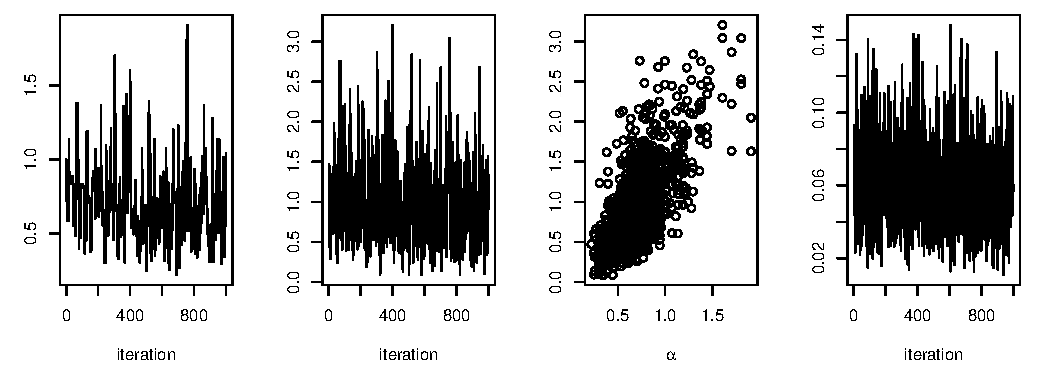
\includegraphics[width=\maxwidth]{figure/mcmcPump-1} 
\begin{kframe}\begin{alltt}
\hlkwd{acf}\hlstd{(samples[,} \hlstr{"alpha"}\hlstd{])} \hlcom{## plot autocorrelation of alpha sample}
\hlkwd{acf}\hlstd{(samples[,} \hlstr{"beta"}\hlstd{])}  \hlcom{## plot autocorrelation of beta  sample}
\end{alltt}
\end{kframe}
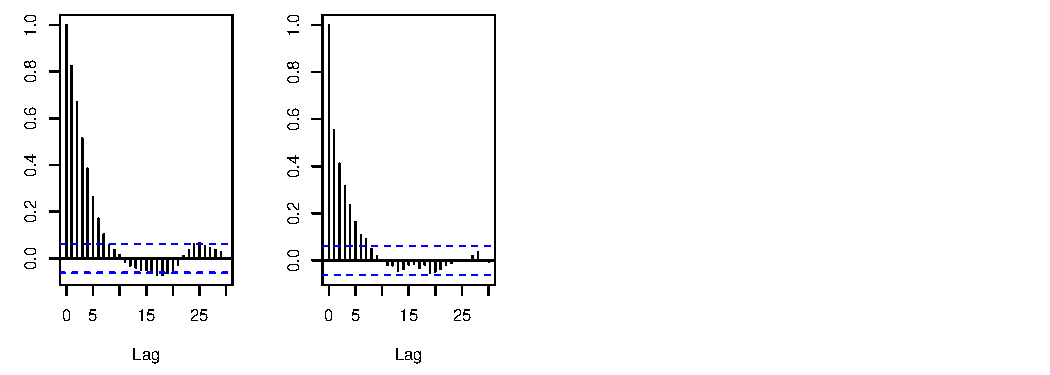
\includegraphics[width=\maxwidth]{figure/mcmcPump-2} 

\end{knitrout}

Notice the posterior correlation between \cd{alpha} and \cd{beta}.
A measure of the mixing for each is the 
autocorrelation for each parameter, shown by the \cd{acf} plots. 

\section{Customizing the MCMC}
\label{sec:customizing-mcmc}

Let's add an adaptive
block sampler on \cd{alpha} and \cd{beta} jointly and see if that
improves the mixing. 

\begin{knitrout}
\definecolor{shadecolor}{rgb}{0.969, 0.969, 0.969}\color{fgcolor}\begin{kframe}
\begin{alltt}
\hlstd{pumpConf}\hlopt{$}\hlkwd{addSampler}\hlstd{(}\hlkwc{target} \hlstd{=} \hlkwd{c}\hlstd{(}\hlstr{"alpha"}\hlstd{,} \hlstr{"beta"}\hlstd{),} \hlkwc{type} \hlstd{=} \hlstr{"RW_block"}\hlstd{,}
                    \hlkwc{control} \hlstd{=} \hlkwd{list}\hlstd{(}\hlkwc{adaptInterval} \hlstd{=} \hlnum{100}\hlstd{))}

\hlstd{pumpMCMC2} \hlkwb{<-} \hlkwd{buildMCMC}\hlstd{(pumpConf)}

\hlcom{# need to reset the nimbleFunctions in order to add the new MCMC}
\hlstd{CpumpNewMCMC} \hlkwb{<-} \hlkwd{compileNimble}\hlstd{(pumpMCMC2,} \hlkwc{project}  \hlstd{= pump,}
                              \hlkwc{resetFunctions} \hlstd{=} \hlnum{TRUE}\hlstd{)}

\hlkwd{set.seed}\hlstd{(}\hlnum{1}\hlstd{)}
\hlstd{CpumpNewMCMC}\hlopt{$}\hlkwd{run}\hlstd{(niter)}
\end{alltt}
\begin{verbatim}
## NULL
\end{verbatim}
\begin{alltt}
\hlstd{samplesNew} \hlkwb{<-} \hlkwd{as.matrix}\hlstd{(CpumpNewMCMC}\hlopt{$}\hlstd{mvSamples)}

\hlkwd{par}\hlstd{(}\hlkwc{mfrow} \hlstd{=} \hlkwd{c}\hlstd{(}\hlnum{1}\hlstd{,} \hlnum{4}\hlstd{),} \hlkwc{mai} \hlstd{=} \hlkwd{c}\hlstd{(}\hlnum{.6}\hlstd{,} \hlnum{.4}\hlstd{,} \hlnum{.1}\hlstd{,} \hlnum{.2}\hlstd{))}
\hlkwd{plot}\hlstd{(samplesNew[ ,} \hlstr{"alpha"}\hlstd{],} \hlkwc{type} \hlstd{=} \hlstr{"l"}\hlstd{,} \hlkwc{xlab} \hlstd{=} \hlstr{"iteration"}\hlstd{,}
     \hlkwc{ylab} \hlstd{=} \hlkwd{expression}\hlstd{(alpha))}
\hlkwd{plot}\hlstd{(samplesNew[ ,} \hlstr{"beta"}\hlstd{],} \hlkwc{type} \hlstd{=} \hlstr{"l"}\hlstd{,} \hlkwc{xlab} \hlstd{=} \hlstr{"iteration"}\hlstd{,}
     \hlkwc{ylab} \hlstd{=} \hlkwd{expression}\hlstd{(beta))}
\hlkwd{plot}\hlstd{(samplesNew[ ,} \hlstr{"alpha"}\hlstd{], samplesNew[ ,} \hlstr{"beta"}\hlstd{],} \hlkwc{xlab} \hlstd{=} \hlkwd{expression}\hlstd{(alpha),}
     \hlkwc{ylab} \hlstd{=} \hlkwd{expression}\hlstd{(beta))}
\hlkwd{plot}\hlstd{(samplesNew[ ,} \hlstr{"theta[1]"}\hlstd{],} \hlkwc{type} \hlstd{=} \hlstr{"l"}\hlstd{,} \hlkwc{xlab} \hlstd{=} \hlstr{"iteration"}\hlstd{,}
     \hlkwc{ylab} \hlstd{=} \hlkwd{expression}\hlstd{(theta[}\hlnum{1}\hlstd{]))}
\end{alltt}
\end{kframe}
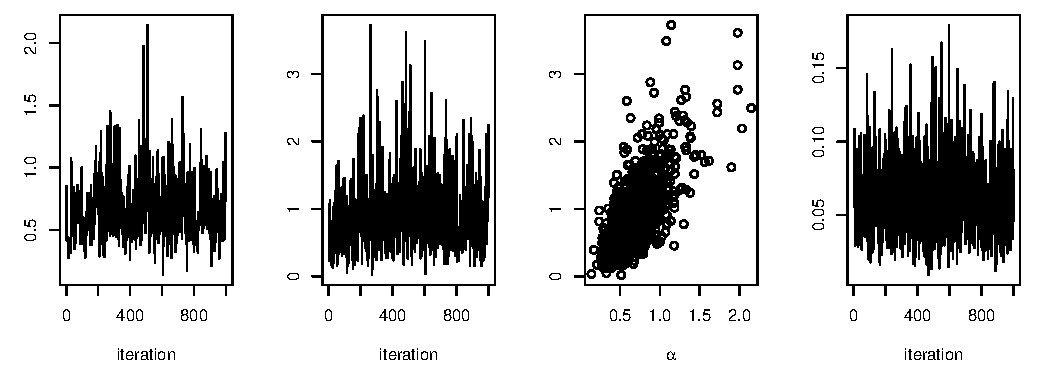
\includegraphics[width=\maxwidth]{figure/mcmcPump2-1} 
\begin{kframe}\begin{alltt}
\hlkwd{acf}\hlstd{(samplesNew[,} \hlstr{"alpha"}\hlstd{])} \hlcom{## plot autocorrelation of alpha sample}
\hlkwd{acf}\hlstd{(samplesNew[,} \hlstr{"beta"}\hlstd{])}  \hlcom{## plot autocorrelation of beta  sample}
\end{alltt}
\end{kframe}
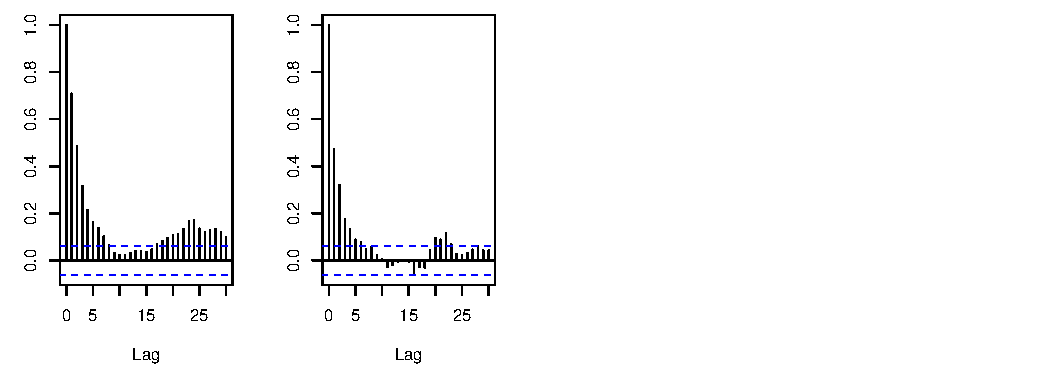
\includegraphics[width=\maxwidth]{figure/mcmcPump2-2} 

\end{knitrout}

We can see that the block sampler has decreased the 
autocorrelation for both \cd{alpha} and \cd{beta}.  Of course these
are just short runs, and what we are really interested in is the
effective sample size of the MCMC per computation time, but that's not
the point of this example.

Once you learn the MCMC system, you can write your own samplers and
include them.  The entire system is written in nimbleFunctions.

\section{Running MCEM}
\label{sec:running-mcem}

NIMBLE is a system for working with algorithms, not just an MCMC engine. So let's try maximizing the marginal likelihood for \cd{alpha} and \cd{beta} using Monte Carlo Expectation Maximization\footnote{Note that for this model, one could analytically integrate over \cd{theta} and then numerically maximize the resulting marginal likelihood.}. 

\begin{knitrout}
\definecolor{shadecolor}{rgb}{0.969, 0.969, 0.969}\color{fgcolor}\begin{kframe}
\begin{alltt}
\hlstd{pump2} \hlkwb{<-} \hlstd{pump}\hlopt{$}\hlkwd{newModel}\hlstd{()}

\hlstd{box} \hlkwb{=} \hlkwd{list}\hlstd{(} \hlkwd{list}\hlstd{(}\hlkwd{c}\hlstd{(}\hlstr{"alpha"}\hlstd{,}\hlstr{"beta"}\hlstd{),} \hlkwd{c}\hlstd{(}\hlnum{0}\hlstd{,} \hlnum{Inf}\hlstd{)))}

\hlstd{pumpMCEM} \hlkwb{<-} \hlkwd{buildMCEM}\hlstd{(}\hlkwc{model} \hlstd{= pump2,} \hlkwc{latentNodes} \hlstd{=} \hlstr{"theta[1:10]"}\hlstd{,}
                      \hlkwc{boxConstraints} \hlstd{= box)}

\hlcom{# Note: buildMCEM returns an R function that contains a}
\hlcom{# nimbleFunction rather than a nimble function. That is why}
\hlcom{# pumpMCEM() is used here instead of pumpMCEM$run().}
\hlstd{pumpMLE} \hlkwb{<-} \hlstd{pumpMCEM}\hlopt{$}\hlkwd{run}\hlstd{()}
\end{alltt}
\begin{verbatim}
## Iteration Number: 1.
## Current number of MCMC iterations: 1000.
## Parameter Estimates: 
##     alpha      beta 
## 0.8160625 1.1230921 
## Convergence Criterion: 1.001.
## Iteration Number: 2.
## Current number of MCMC iterations: 1000.
## Parameter Estimates: 
##     alpha      beta 
## 0.8045037 1.1993128 
## Convergence Criterion: 0.0223464.
## Monte Carlo error too big: increasing MCMC sample size.
## Iteration Number: 3.
## Current number of MCMC iterations: 1250.
## Parameter Estimates: 
##     alpha      beta 
## 0.8203178 1.2497067 
## Convergence Criterion: 0.004913688.
## Monte Carlo error too big: increasing MCMC sample size.
## Monte Carlo error too big: increasing MCMC sample size.
## Monte Carlo error too big: increasing MCMC sample size.
## Iteration Number: 4.
## Current number of MCMC iterations: 3032.
## Parameter Estimates: 
##     alpha      beta 
## 0.8226618 1.2602452 
## Convergence Criterion: 0.0004201047.
\end{verbatim}
\begin{alltt}
\hlstd{pumpMLE}
\end{alltt}
\begin{verbatim}
##     alpha      beta 
## 0.8226618 1.2602452
\end{verbatim}
\end{kframe}
\end{knitrout}


Both estimates are within 0.01 of the values reported by
\citet{George_Makov_Smith_1993}\footnote{Table 2 of the paper accidentally swapped the two estimates.}. %\footnote{George, E.I., Makov, U.E. \& Smith,
%  A.F.M. 1993. Conjugate likelihood
 % distributions. \textit{Scand. J. Statist.} \textbf{20}:147-156.
 % Their numbers were accidentally swapped in Table 2.}.  
Some discrepancy is to be expected since it is a Monte Carlo algorithm.

\section{Creating your own functions}
\label{sec:creating-your-own}



Now let's see an example of writing our own algorithm and using it on
the model. We'll do something simple: simulating multiple values for a
designated set of nodes and calculating every part of the model that
depends on them. More details on programming in NIMBLE are in Part \ref{part:programming}.

Here is our \nm{nimbleFunction}:
\begin{knitrout}
\definecolor{shadecolor}{rgb}{0.969, 0.969, 0.969}\color{fgcolor}\begin{kframe}
\begin{alltt}
\hlstd{simNodesMany} \hlkwb{<-} \hlkwd{nimbleFunction}\hlstd{(}
    \hlkwc{setup} \hlstd{=} \hlkwa{function}\hlstd{(}\hlkwc{model}\hlstd{,} \hlkwc{nodes}\hlstd{) \{}
        \hlstd{mv} \hlkwb{<-} \hlkwd{modelValues}\hlstd{(model)}
        \hlstd{deps} \hlkwb{<-} \hlstd{model}\hlopt{$}\hlkwd{getDependencies}\hlstd{(nodes)}
        \hlstd{allNodes} \hlkwb{<-} \hlstd{model}\hlopt{$}\hlkwd{getNodeNames}\hlstd{()}
    \hlstd{\},}
    \hlkwc{run} \hlstd{=} \hlkwa{function}\hlstd{(}\hlkwc{n} \hlstd{=} \hlkwd{integer}\hlstd{()) \{}
        \hlkwd{resize}\hlstd{(mv, n)}
        \hlkwa{for}\hlstd{(i} \hlkwa{in} \hlnum{1}\hlopt{:}\hlstd{n) \{}
            \hlstd{model}\hlopt{$}\hlkwd{simulate}\hlstd{(nodes)}
            \hlstd{model}\hlopt{$}\hlkwd{calculate}\hlstd{(deps)}
            \hlkwd{copy}\hlstd{(}\hlkwc{from} \hlstd{= model,} \hlkwc{nodes} \hlstd{= allNodes,}
                 \hlkwc{to} \hlstd{= mv,} \hlkwc{rowTo} \hlstd{= i,} \hlkwc{logProb} \hlstd{=} \hlnum{TRUE}\hlstd{)}
        \hlstd{\}}
    \hlstd{\})}

\hlstd{simNodesTheta1to5} \hlkwb{<-} \hlkwd{simNodesMany}\hlstd{(pump,} \hlstr{"theta[1:5]"}\hlstd{)}
\hlstd{simNodesTheta6to10} \hlkwb{<-} \hlkwd{simNodesMany}\hlstd{(pump,} \hlstr{"theta[6:10]"}\hlstd{)}
\end{alltt}
\end{kframe}
\end{knitrout}

Here are a few things to notice about the nimbleFunction.
\begin{enumerate}
\item The \cd{setup} function is written in R.  It creates relevant
  information specific to our model for use in the run-time code.  
\item The \cd{setup} code creates a \nm{modelValues} object to hold multiple sets of
  values for variables  in the model provided.
\item The \cd{run} function is written in NIMBLE.  It carries out the
  calculations using the information determined once for each set of
  \cd{model} and \cd{nodes} arguments by the setup
  code. The run-time code is what will be compiled.
\item The \cd{run} code requires type information about the argument
  \cd{n}.  In this case it is a scalar integer.  
\item The for-loop looks just like R, but only sequential integer
  iteration is allowed.
\item The functions \cd{calculate} and \cd{simulate}, which were
  introduced above in R, can be used in NIMBLE.
\item The special function \cd{copy} is used here to record values
  from the model into the modelValues object.  
\item Multiple instances, or ``specializations'', can be made by
  calling \cd{simNodesMany} with different arguments.  Above, \cd{simNodesTheta1to5} has
  been made by calling \cd{simNodesMany} with the \cd{pump} model and
  nodes \cd{"theta[1:5]"} as inputs to
  the \cd{setup} function, while \cd{simNodesTheta6to10} differs by
  providing \cd{"theta[6:10]"} as an argument.  The returned objects
  are objects of a uniquely
  generated R reference class with fields (member data) for the results of the
  \cd{setup} code and a \cd{run} method (member function). 
   % Arbitrary other methods can be provided with a \cd{methods} argument, following the syntax of R's \cd{setRefClass} function.
  % NOTE: CJP removed previous sentence as I think it is too involved for the lightning intro - CJP
\end{enumerate}

By the way, \cd{simNodesMany} is very similar to a standard
\cd{nimbleFunction} provided with nimble, \cd{simNodesMV}.

Now let's execute this nimbleFunction in R, before compiling it.

\begin{knitrout}
\definecolor{shadecolor}{rgb}{0.969, 0.969, 0.969}\color{fgcolor}\begin{kframe}
\begin{alltt}
\hlkwd{set.seed}\hlstd{(}\hlnum{1}\hlstd{)}  \hlcom{## make the calculation repeatable}
\hlstd{pump}\hlopt{$}\hlstd{alpha} \hlkwb{<-} \hlstd{pumpMLE[}\hlnum{1}\hlstd{]}
\hlstd{pump}\hlopt{$}\hlstd{beta} \hlkwb{<-} \hlstd{pumpMLE[}\hlnum{2}\hlstd{]}
\hlcom{## make sure to update deterministic dependencies of the altered nodes}
\hlstd{pump}\hlopt{$}\hlkwd{calculate}\hlstd{(pump}\hlopt{$}\hlkwd{getDependencies}\hlstd{(}\hlkwd{c}\hlstd{(}\hlstr{"alpha"}\hlstd{,}\hlstr{"beta"}\hlstd{),} \hlkwc{determOnly} \hlstd{=} \hlnum{TRUE}\hlstd{))}
\end{alltt}
\begin{verbatim}
## [1] 0
\end{verbatim}
\begin{alltt}
\hlstd{saveTheta} \hlkwb{<-} \hlstd{pump}\hlopt{$}\hlstd{theta}
\hlstd{simNodesTheta1to5}\hlopt{$}\hlkwd{run}\hlstd{(}\hlnum{10}\hlstd{)}
\hlstd{simNodesTheta1to5}\hlopt{$}\hlstd{mv[[}\hlstr{"theta"}\hlstd{]][}\hlnum{1}\hlopt{:}\hlnum{2}\hlstd{]}
\end{alltt}
\begin{verbatim}
## [[1]]
##  [1] 0.21829875 1.93210969 0.62296551 0.34197267 3.45729601
##  [6] 1.15835525 0.99001994 0.30737332 0.09461909 0.15720154
## 
## [[2]]
##  [1] 0.82759981 0.08784057 0.34414959 0.29521943 0.14183505
##  [6] 1.15835525 0.99001994 0.30737332 0.09461909 0.15720154
\end{verbatim}
\begin{alltt}
\hlstd{simNodesTheta1to5}\hlopt{$}\hlstd{mv[[}\hlstr{"logProb_x"}\hlstd{]][}\hlnum{1}\hlopt{:}\hlnum{2}\hlstd{]}
\end{alltt}
\begin{verbatim}
## [[1]]
##  [1] -10.250111 -26.921849 -25.630612 -15.594173 -11.217566
##  [6]  -7.429868  -1.000761  -1.453644  -9.840589 -39.096527
## 
## [[2]]
##  [1] -61.043876  -1.057668 -11.060164 -11.761432  -3.425282
##  [6]  -7.429868  -1.000761  -1.453644  -9.840589 -39.096527
\end{verbatim}
\end{kframe}
\end{knitrout}

In this code we have initialized the values of \cd{alpha} and \cd{beta}
to their MLE and then recorded the \cd{theta} values to use below.  Then we
have requested 10 simulations from
\cd{simNodesTheta1to5}.  Shown are the first two simulation results
for \cd{theta} and the log probabilities of \cd{x}.  Notice that
\cd{theta[6:10]} and the corresponding log probabilities for \cd{x[6:10]} are unchanged because the nodes being simulated are only
\cd{theta[1:5]}.  In R, this function runs slowly.

Finally, let's compile the function and run that version.

\begin{knitrout}
\definecolor{shadecolor}{rgb}{0.969, 0.969, 0.969}\color{fgcolor}\begin{kframe}
\begin{alltt}
\hlstd{CsimNodesTheta1to5} \hlkwb{<-} \hlkwd{compileNimble}\hlstd{(simNodesTheta1to5,}
                                    \hlkwc{project}  \hlstd{= pump,} \hlkwc{resetFunctions} \hlstd{=} \hlnum{TRUE}\hlstd{)}
\hlstd{Cpump}\hlopt{$}\hlstd{alpha} \hlkwb{<-} \hlstd{pumpMLE[}\hlnum{1}\hlstd{]}
\hlstd{Cpump}\hlopt{$}\hlstd{beta} \hlkwb{<-} \hlstd{pumpMLE[}\hlnum{2}\hlstd{]}
\hlstd{Cpump}\hlopt{$}\hlkwd{calculate}\hlstd{(Cpump}\hlopt{$}\hlkwd{getDependencies}\hlstd{(}\hlkwd{c}\hlstd{(}\hlstr{"alpha"}\hlstd{,}\hlstr{"beta"}\hlstd{),} \hlkwc{determOnly} \hlstd{=} \hlnum{TRUE}\hlstd{))}
\end{alltt}
\begin{verbatim}
## [1] 0
\end{verbatim}
\begin{alltt}
\hlstd{Cpump}\hlopt{$}\hlstd{theta} \hlkwb{<-} \hlstd{saveTheta}

\hlkwd{set.seed}\hlstd{(}\hlnum{1}\hlstd{)}
\hlstd{CsimNodesTheta1to5}\hlopt{$}\hlkwd{run}\hlstd{(}\hlnum{10}\hlstd{)}
\end{alltt}
\begin{verbatim}
## NULL
\end{verbatim}
\begin{alltt}
\hlstd{CsimNodesTheta1to5}\hlopt{$}\hlstd{mv[[}\hlstr{"theta"}\hlstd{]][}\hlnum{1}\hlopt{:}\hlnum{2}\hlstd{]}
\end{alltt}
\begin{verbatim}
## [[1]]
##  [1] 0.21829875 1.93210969 0.62296551 0.34197267 3.45729601
##  [6] 1.15835525 0.99001994 0.30737332 0.09461909 0.15720154
## 
## [[2]]
##  [1] 0.82759981 0.08784057 0.34414959 0.29521943 0.14183505
##  [6] 1.15835525 0.99001994 0.30737332 0.09461909 0.15720154
\end{verbatim}
\begin{alltt}
\hlstd{CsimNodesTheta1to5}\hlopt{$}\hlstd{mv[[}\hlstr{"logProb_x"}\hlstd{]][}\hlnum{1}\hlopt{:}\hlnum{2}\hlstd{]}
\end{alltt}
\begin{verbatim}
## [[1]]
##  [1] -10.250111 -26.921849 -25.630612 -15.594173 -11.217566
##  [6]  -2.782156  -1.042151  -1.004362  -1.894675  -3.081102
## 
## [[2]]
##  [1] -61.043876  -1.057668 -11.060164 -11.761432  -3.425282
##  [6]  -2.782156  -1.042151  -1.004362  -1.894675  -3.081102
\end{verbatim}
\end{kframe}
\end{knitrout}

Given the same initial values and the same random number generator
seed, we got identical results for \cd{theta[1:5]} and their dependencies, but it happened much faster.



%% See http://yihui.name/knitr/demo/child/ for documentation on the parent/child document system of knitr



\chapter{More introduction}

Now that we have shown a brief example, we will introduce more about
the concepts and design of NIMBLE.  

One of the most important concepts behind NIMBLE is to allow a
combination of high-level processing in R and low-level processing in
C++.  For example, when we write a Metropolis-Hastings MCMC sampler in
the NIMBLE language, the inspection of the model structure related to
one node is done in R, and the actual sampler calculations are done in
C++.  This separation between \textit{setup} and \textit{run} steps
will become clearer as we go.


\section{NIMBLE adopts and extends the BUGS language for specifying models}

We adopted the BUGS language, and we have extended it to make it more
flexible. The BUGS language became widely used in WinBUGS, then in
OpenBUGS and JAGS.  These systems all provide automatically-generated
MCMC algorithms, but we have adopted only the language for describing
models, not their systems for generating MCMCs.  

NIMBLE extends BUGS by:
\begin{enumerate}
\item allowing you to write new functions and
distributions and use them in BUGS models;
\item allowing you to define multiple models in the same code using
  conditionals evaluated when the BUGS code is processed;
\item supporting a variety of more flexible syntax such as R-like
  named parameters and more general algebraic expressions.
\end{enumerate}
By supporting new functions and distributions, NIMBLE makes BUGS an
extensible language, which is a major departure from previous
packages that implement BUGS.  

We adopted BUGS because it has been so successful, with over 30,000
users by the time they stopped counting
\citep{Lunn_Spiegelhalter_Thomas_Best_2009}.  Many papers and books
provide BUGS code as a way to document their statistical models. We
describe NIMBLE's version of BUGS later.  The web sites for WinBUGS,
OpenBUGS and JAGS provide other useful documntation on writing models
in BUGS.  For the most part, if you have BUGS code, you can try
NIMBLE.

NIMBLE does several things with BUGS code:
\begin{enumerate}
\item NIMBLE creates a \nm{model definition} object that knows
  everything about the variables and their relationships written in
  the BUGS code.  Usually you'll ignore the \nm{model definition}
  and let NIMBLE's default options take you directly to the next step.
\item NIMBLE creates a model object\footnote{or multiple model
    objects}.  This can be used to
  manipulate variables and operate the model from R.  Operating the
  model includes calculating, simulating, or querying the log
  probability value of model nodes. These basic capabilities, along
  with the tools to query model structure, allow one to write
  programs that use the model and adapt to its structure.
\item When you're ready, NIMBLE can generate customized C++ code
  representing the model, compile the C++, load it back into R, and
  provide a new model object that uses the compiled model
  internally.  We use the word ``compile'' to refer to all of these
  steps together.
\end{enumerate}

As an example of how radical a departure NIMBLE is from previous BUGS
implementations, consider a situation where you want to simulate new
data from a model written in BUGS code.  Since NIMBLE creates model
objects that you can control from R, simulating new data is trivial.
With previous BUGS-based packages, this isn't possible.

More information about specifying and manipulating models is in
Chapters \ref{cha:building-models} and \ref{cha:using-bugs-models}.

\section{nimbleFunctions for writing algorithms}
\label{sec:nimble-lang-writ}

NIMBLE provides \nm{nimbleFunction}s for writing functions that can
(but don't have to) use BUGS models.  The main ways that nimbleFunctions can use
BUGS models are:

\begin{enumerate}
\item inspecting the structure of a model, such as determining the
  dependencies between variables, in order to do the right
  calculations with each model;
\item accessing values of the model's variables;
\item controlling execution of the model's probability calculations
  or corresponding simulations;
\item managing \nm{modelValues} data structures for multiple sets of
  model values and probabilities.
\end{enumerate}

In fact, the calculations of the model are themselves constructed as
nimbleFunctions, as are the algorithms provided in
NIMBLE's algorithm library\footnote{That's why it's easy to use new
  functions and distributions written as nimbleFunctions in BUGS code.}.

Programming with nimbleFunctions involves a fundamental distinction
between two stages of processing:
\begin{enumerate}

\item A \nm{setup} function within a nimbleFunction gives the steps
  that need to happen only once for each new situation (e.g., for each
  new model).  Typically such steps include inspecting the model's
  variables and their relationships, such as determining which parts
  of a model will need to be calculated for a MCMC sampler. Setup
  functions are executed in R and never compiled.

\item One or more \nm{run} functions within a nimbleFunction give
  steps that need to happen multiple times using the results of the
  setup function, such as the iterations of a MCMC sampler.
  Formally, run code is written in the NIMBLE language, which you
  can think of as a small subset of R along with features for
  operating models and related data structures.  The NIMBLE language
  is what the NIMBLE compiler can automatically turn into C++ as part
  of a compiled nimbleFunction.
\end{enumerate}

What NIMBLE does with a nimbleFunction is similar to what it does
with a BUGS model:
\begin{enumerate}
\item NIMBLE creates a working R version of the nimbleFunction.
  This is most useful for debugging (Section \ref{sec:debugging}).
\item When you are ready, NIMBLE can generate C++ code, compile it,
  load it back into R and give you new objects that use the compiled
  C++ internally.  Again, we refer to these steps all together as ``compilation.''  The behavior of compiled nimbleFunctions is
  usually very similar, but not identical, to their uncompiled
  counterparts.
\end{enumerate}

If you are familiar with object-oriented programming, you can think of
a nimbleFunction as a class definition. The setup function
initializes a new object and run functions are class methods.
Member data are determined automatically as the objects from a
setup function needed in run functions.  If no setup
function is provided, the nimbleFunction corresponds to a simple
(compilable) function rather than a class.

More about writing algorithms is in Chapter \ref{cha:progr-with-models}.

\section{The NIMBLE algorithm library}
\label{sec:nimble-algor-libr}

In Version \ver, the NIMBLE algorithm library includes:

\begin{enumerate}
\item MCMC with samplers including conjugate (Gibbs), slice, adaptive
  random walk (with options for reflection or sampling on a log
  scale), adaptive block random walk, and elliptical slice, among others. You can
  modify sampler choices and configurations from R before compiling
  the MCMC.  You can also write new samplers as nimbleFunctions.
\item A set of particle filter (sequential Monte Carlo) methods
  including a basic bootstrap filter, auxiliary particle filter, and
  Liu-West filter.
\item An ascent-based Monte Carlo Expectation Maximization (MCEM)
  algorithm.
\item A variety of basic functions that can be used as programming
  tools for larger algorithms.  These include:
  \begin{enumerate}
  \item A likelihood function for arbitrary parts of any model.
  \item Functions to simulate one or many sets of values for arbitrary
    parts of any model.
  \item Functions to calculate the summed log probability (density)
    for one or many sets of values for arbitrary parts of any model
    along with stochastic dependencies in the model structure.
  \end{enumerate}

\end{enumerate}

% Someone (Perry?) added this comment: Add references where appropriate. Chris suggests we probably don't need refs here as we are referring to very widely-known algorithms.
 
More about the NIMBLE algorithm library is in Chapter \ref{cha:algos-provided}.


%% See http://yihui.name/knitr/demo/child/ for documentation on the parent/child document system of knitr



\chapter{Installing NIMBLE}
\label{cha:installing-nimble}

\section{Requirements to run NIMBLE}
\label{sec:requ-run-nimble}

You can run NIMBLE on any of the three common operating systems: Linux, Mac OS X, or Windows. 

The following are required to run NIMBLE.

\begin{enumerate}
\item \href{http://www.cran.r-project.org}{R}, of course.
\item The \href{http://www.cran.r-project.org/web/packages/igraph/index.html}{igraph} and  \href{http://www.cran.r-project.org/web/packages/coda/index.html}{coda} R packages.
\item A working C++ compiler that NIMBLE can use from R on your system.  There are
  standard open-source C++ compilers that the R community has already
  made easy to install.  See Section \ref{sec:compiler} for
  instructions.  You don't need to know anything about C++ to use
  NIMBLE.  This must be done before installing NIMBLE.

\end{enumerate}

NIMBLE also uses a couple of C++ libraries that you don't need to install, as they will already be on your system or are provided by NIMBLE.
\begin{enumerate}
\item The \href{http://eigen.tuxfamily.org}{Eigen} C++ library
  for linear algebra.  This comes with NIMBLE, or you can use your own copy.
\item The BLAS and LAPACK numerical libraries.  These come with
  R, but see Section \ref{sec:blas} for how to use a faster version of the BLAS.
\end{enumerate}

Most fairly recent versions of these requirements should work. 
% [look into giving more detailed version requirements]


\section{Installing a C++ compiler for NIMBLE to use}
\label{sec:compiler}

NIMBLE needs a C++ compiler and the standard utility \nm{make} in
order to generate and compile C++ for models and algorithms.\footnote{This differs from most packages, which might need a C++ compiler
  only when the package is built.  If you normally install R packages using
  \cd{install.packages} on Windows or OS X, the package arrives
  already built to your system.}

\subsection{OS X}
On OS X, you should install \nm{Xcode}.  The command-line tools, which are
available as a smaller installation, should be sufficient. This is freely available from the
\href{https://developer.apple.com/xcode/downloads/}{Apple developer
  site} and the
\href{https://itunes.apple.com/us/app/xcode/id497799835?ls=1&mt=12}{App Store}.

% Perry asked if App Store link is stable - Chris checked and it seems fine for now (and is the top hit on a Google search ...

For the compiler to work correctly for OS X, the installed R must be
for the correct version of OS X.  For example, R for Snow Leopard (OS
X version 10.8) will attempt to use an incorrect C++ compiler if the
installed OS X is actually version 10.9 or higher.

% PdV -- rewrote this -- need to check example.

In the somewhat unlikely event you want to install from the source package rather than the CRAN binary package, the easiest approach is to use the source package provided at \href{http://R-nimble.org}{R-nimble.org}. If you do want to install from the source package provided by CRAN, you'll need to install \href{http://r.research.att.com/libs/gfortran-4.8.2-darwin13.tar.bz2}{this gfortran package}.

\subsection{Linux}
On Linux, you can install the GNU compiler suite (\nm{gcc}/\nm{g++}). 
You can use the package manager to install pre-built binaries.
On Ubuntu, the following command will install or update \nm{make}, \nm{gcc} and \nm{libc}.
\begin{knitrout}
\definecolor{shadecolor}{rgb}{0.969, 0.969, 0.969}\color{fgcolor}\begin{kframe}
\begin{alltt}
sudo apt-get install build-essential
\end{alltt}
\end{kframe}
\end{knitrout}

\subsection{Windows}
On Windows, you should download and install \file{Rtools.exe}
available from \url{http://cran.r-project.org/bin/windows/Rtools/}.
Select the appropriate executable corresponding to your version of R
(and follow the urge to update your version of R if you notice it
is not the most recent).  This installer leads you through several
``pages''.  We think you can accept the defaults with one exception:
check the PATH checkbox (page 5) so that the installer will add the
location of the C++ compiler and related tools to your system's PATH,
ensuring that R can find them.  After you click ``Next'', you will get
a page with a window for customizing the new PATH variable.  You
shouldn't need to do anything there, so you can simply click ``Next''
again.

The checkbox for the ``R 2.15+ toolchain'' (page 4) must be checked
(in order to have \nm{gcc}/\nm{g++}, \nm{make}, etc. installed).  This
should be checked by default.

\section{Installing the NIMBLE package}

Since NIMBLE is an R package, you can install it in the usual way, via
\\\cd{install.packages("nimble")} in R or using the \cd{R CMD INSTALL}
method if you download the package source directly. 

NIMBLE can also be obtained from the \href{http://r-nimble.org}{NIMBLE website}. To install from our website, please see our \href{http://r-nimble.org/download}{Download page} for the specific invocation of \cd{install.packages}.


\subsection{Problems with installation}
We have tested the installation on the three commonly used platforms
-- OS X, Linux, Windows\footnote{We've tested NIMBLE on Windows 7, 8
  and 10.}.  We don't anticipate problems with installation,
but we want to hear about any and help resolve them. 
Please post about installation problems to the \href{https://groups.google.com/forum/#!forum/nimble-users}{nimble-users Google group} or 
email \href{mailto:nimble.stats@gmail.com}{nimble.stats@gmail.com}.

\section{Customizing your installation}

For most installations, you can ignore low-level details.
However, there are some options that some users may want to utilize.

\subsection{Using your own copy of Eigen}
%\subsection{Finding the Eigen Header Files}
NIMBLE uses the Eigen C++ template library for linear algebra.  Version 3.2.1
of Eigen is included in the NIMBLE package and that version will be
used unless the package's configuration script finds another version
on the machine.  This works well, and the following is only relevant
if you want to use a different (e.g., newer) version.

The configuration script looks in the standard include directories,
e.g. \cd{/usr/include} and \cd{/usr/local/include} for the header file \cd{Eigen/Dense}.
You can specify a particular location in either of two ways:
\begin{enumerate}
  \item Set the environment variable \cd{EIGEN\_DIR} before installing the R
    package,  e.g., \cd{export EIGEN\_DIR=/usr/include/eigen3} in the bash shell.
  \item Use \\
    \verb|R CMD INSTALL --configure-args='--with-eigen=/path/to/eigen' \| \\
    \verb|nimble_VERSION.tar.gz| \\
      or \\ \cd{install.packages("nimble", configure.args = "--with-eigen=/path/to/eigen")}.
\end{enumerate}  
In these cases, the directory should be the full path to the directory that
contains the Eigen directory, e.g., \cd{/usr/include/eigen3}. It is not the full path to the Eigen
directory itself, i.e., NOT \cd{/usr/include/eigen3/Eigen}.


\subsection{Using libnimble}
NIMBLE generates specialized C++ code for user-specified models and nimbleFunctions.
This code uses some NIMBLE C++ library classes and functions.
By default, on Linux the library code is compiled once as a linkable
library - \nm{libnimble.so}. This single instance of the library is then linked 
with the code for each generated model. In contrast, the default for Windows and Mac OS X
is to compile the library code as a static library - \nm{libnimble.a} - that is compiled into each model's and each algorithm's own dynamically loadable library (DLL). This does repeat the same code across models and so occupies more memory. There may be a marginal speed advantage. 
If one would like to enable the linkable library in place of the static library (do this only on Mac OS X and other UNIX variants and not on Windows), one can install the source package with the configuration argument \cd{--enable-dylib} set to true. First obtain the NIMBLE source package (which will have the extension \cd{.tar.gz} from \href{http://r-nimble.org/download}{our website} and then install as follows, replacing \cd{VERSION} with the appropriate version number:

\verb|R CMD INSTALL --configure-args='--enable-dylib=true' nimble_VERSION.tar.gz|

\subsection{BLAS and LAPACK}
\label{sec:blas}

NIMBLE also uses BLAS and LAPACK for some of its linear algebra (in
particular calculating density values and generating random samples
from multivariate distributions). NIMBLE will use the same BLAS and
LAPACK installed on your system that R uses. Note that a fast (and
where appropriate, threaded) BLAS can greatly increase the speed of
linear algebra calculations. See Section A.3.1 of the \href{https://cran.r-project.org/doc/manuals/r-release/R-admin.html}{R Installation and Administration manual} available on CRAN for more details on providing a fast BLAS for your R installation. 

\subsection{Customizing compilation of the NIMBLE-generated C++}

For each model or nimbleFunction, NIMBLE can generate and compile C++.
To compile generated C++, NIMBLE makes system calls starting with
\cd{R CMD SHLIB} and therefore uses the regular R configuration in
\verb|${R_HOME}/etc/${R_ARCH}/Makeconf|. NIMBLE places a
\file{Makevars} file in the directory in which the code is generated,
and \verb|R CMD SHLIB| uses this file as usual.

In all but specialized cases, the general compilation mechanism will
suffice. However, one can customize this.  One can specify the
location of an alternative \file{Makevars} (or \file{Makevars.win})
file to use.  Such an alternative file should define the variables \cd{PKG\_CPPFLAGS} and
\cd{PKG\_LIBS}.  These should contain, respectively, the pre-processor flag
to locate the NIMBLE include directory, and the necessary
libraries to link against (and their location as necessary),
e.g., \nm{Rlapack} and \nm{Rblas} on Windows, and \nm{libnimble}.
Advanced users can also change their default compilers by editing the
\nm{Makevars} file, see Section 1.2.1 of the \href{https://cran.r-project.org/doc/manuals/r-release/R-exts.html}{Writing R Extensions manual} available on CRAN.


Use of this file allows users to specify additional compilation and
linking flags.  See the Writing R Extensions manual for more details
of how this can be used and what it can contain.

\part{Models in NIMBLE}
\label{part:models}


%% See http://yihui.name/knitr/demo/child/ for documentation on the parent/child document system of knitr





\chapter{Writing models in NIMBLE's dialect of BUGS}
\label{cha:writing-models}

Models in NIMBLE are written using a variation on the BUGS language.
From BUGS code, NIMBLE  creates a model object.  This chapter
describes NIMBLE's version of BUGS.  The next chapter explains how to
build and manipulate model objects.


% With NIMBLE you can also define your own distributions and functions for use in BUGS code; discussion of this functionality is deferred to Chapter \ref{cha:user-defined} as it requires the use of nimbleFunctions. 


\section{Comparison to BUGS dialects supported by WinBUGS, OpenBUGS and JAGS}
\label{sec:supp-feat-bugs}

Many users will come to NIMBLE with some familiarity with WinBUGS,
OpenBUGS, or JAGS, so we start by summarizing how NIMBLE is similar to
and different from those before documenting NIMBLE's version of BUGS
more completely.  In general, NIMBLE aims to be compatible with the
original BUGS language and also JAGS' version.  However, at this
point, there are some features not supported by NIMBLE, and there are
some extensions that are planned but not implemented.

\subsection{Supported features of BUGS and JAGS}

\begin{enumerate}
\item Stochastic and deterministic\footnote{NIMBLE calls non-stochastic nodes ``deterministic'', whereas BUGS calls them ``logical''. NIMBLE uses ``logical'' in the way R does, to refer to boolean (TRUE/FALSE) variables.} node declarations.
\item Most univariate and multivariate distributions.
\item Link functions.
\item Most mathematical functions.
\item ``for'' loops for iterative declarations.
\item Arrays of nodes up to 4 dimensions.
\item Truncation and censoring as in JAGS using the \cd{T()}
  notation and \cd{dinterval}.
\end{enumerate}

\subsection{NIMBLE's Extensions to BUGS and JAGS}
\label{sec:extensions-bugs}

NIMBLE extends the BUGS language in the following ways:

\begin{enumerate}
  \item User-defined functions and distributions -- written as nimbleFunctions -- can be used in model code. See Chapter \ref{cha:user-defined}.
\item Multiple parameterizations for distributions, similar to those  in R, can be used.
\item Named parameters for distributions and functions, similar to R function calls, can be used.
\item Linear algebra, including for vectorized
  calculations of simple algebra, can be used in deterministic declarations.
\item Distribution parameters can be expressions, as in JAGS but not
  in WinBUGS.  Caveat: parameters to \emph{multivariate}
  distributions (e.g., \cd{dmnorm}) cannot be expressions (but an expression can be defined in a separate deterministic expression and the resulting variable then used). % still true. -Perry
 \item Alternative models can be defined from the same model code by
   using if-then-else statements that are evaluated when the model is defined.
\item More flexible indexing of vector nodes within larger variables is allowed.  For example one can place a multivariate normal vector arbitrarily within a higher-dimensional object, not just in the last index.
\item More general constraints can be declared using \cd{dconstraint}, which extends the concept of JAGS' \cd{dinterval}.
 \item Link functions can be used in stochastic, as well as
   deterministic, declarations.\footnote{But beware of the possibility
     of needing to set values for ``lifted'' nodes created by NIMBLE.}
 \item Data values can be reset, and which parts of a model are flagged as data can be changed, allowing one model to be used for different data sets without rebuilding the model each time.
  \end{enumerate}
  
\subsection{Not-yet-supported features of BUGS and JAGS}
\label{sec:not-yet-supported}

In this release, the following are not supported.

\begin{enumerate}
\item Stochastic indices (but see Chapter \ref{cha:user-defined} for a
  description of how you could handle some cases with user-defined
  functions or distributions).
\item The appearance of the same node on the left-hand side of both a
  \cd{<-} and a \cd{$\sim$} declaration (used in WinBUGS for data
  assignment for the value of a stochastic node).
\item Multivariate nodes must appear with brackets, even if they are
    empty. E.g., \cd{x} cannot be multivariate but \cd{x[]} or
    \cd{x[2:5]} can be.
\item NIMBLE generally determines the dimensionality and
  sizes of variables from the BUGS code.  However, when a variable
  appears with blank indices, such as in \cd{x.sum <- sum(x[])},
  and if the dimensions of the variable are not clearly defined in
  other declarations, NIMBLE currently requires that the dimensions of
  x be provided when the model object is created (via \cd{nimbleModel}).
\end{enumerate}

\section{Writing models}

Here we introduce NIMBLE's version of BUGS.  The WinBUGS, OpenBUGS and
JAGS manuals are also useful resources for writing BUGS models,
including many examples.

\subsection{Declaring stochastic and deterministic nodes}

BUGS is a declarative language for graphical (or hierarchical) models.
Most programming languages are imperative, which means a series of
commands will be executed in the order they are written.  A
declarative language like BUGS is more like building a machine before
using it.  Each line declares that a component should be plugged into
the machine, but it doesn't matter in what order they are declared as
long as all the right components are plugged in by the end of the code.

The machine in this case is a graphical model\footnote{Technically, a
  \textit{directed acyclic graph}}.  A \textit{node} (sometimes called
a \textit{vertex}) holds one value, which may be a scalar or a vector.
\textit{Edges} define the relationships between nodes.  A huge variety
of statistical models can be thought of as graphs.  

Here is the code to define and create a simple linear regression model with four observations. 



\begin{knitrout}
\definecolor{shadecolor}{rgb}{0.969, 0.969, 0.969}\color{fgcolor}\begin{kframe}
\begin{alltt}
\hlkwd{library}\hlstd{(nimble)}
\hlstd{mc} \hlkwb{<-} \hlkwd{nimbleCode}\hlstd{(\{}
    \hlstd{intercept} \hlopt{~} \hlkwd{dnorm}\hlstd{(}\hlnum{0}\hlstd{,} \hlkwc{sd} \hlstd{=} \hlnum{1000}\hlstd{)}
    \hlstd{slope} \hlopt{~} \hlkwd{dnorm}\hlstd{(}\hlnum{0}\hlstd{,} \hlkwc{sd} \hlstd{=} \hlnum{1000}\hlstd{)}
    \hlstd{sigma} \hlopt{~} \hlkwd{dunif}\hlstd{(}\hlnum{0}\hlstd{,} \hlnum{100}\hlstd{)}
    \hlkwa{for}\hlstd{(i} \hlkwa{in} \hlnum{1}\hlopt{:}\hlnum{4}\hlstd{) \{}
        \hlstd{predicted.y[i]} \hlkwb{<-} \hlstd{intercept} \hlopt{+} \hlstd{slope} \hlopt{*} \hlstd{x[i]}
        \hlstd{y[i]} \hlopt{~} \hlkwd{dnorm}\hlstd{(predicted.y[i],} \hlkwc{sd} \hlstd{= sigma)}
    \hlstd{\}}
\hlstd{\})}

\hlstd{model} \hlkwb{<-} \hlkwd{nimbleModel}\hlstd{(mc,} \hlkwc{data} \hlstd{=} \hlkwd{list}\hlstd{(}\hlkwc{y} \hlstd{=} \hlkwd{rnorm}\hlstd{(}\hlnum{4}\hlstd{)))}

\hlkwd{library}\hlstd{(igraph)}

\hlstd{layout} \hlkwb{<-} \hlkwd{matrix}\hlstd{(}\hlkwc{ncol} \hlstd{=} \hlnum{2}\hlstd{,} \hlkwc{byrow} \hlstd{=} \hlnum{TRUE}\hlstd{,}
   \hlcom{## These seem to be rescaled to fit in the plot area,}
   \hlcom{## so I'll just use 0-100 as the scale}
                 \hlkwc{data} \hlstd{=} \hlkwd{c}\hlstd{(}\hlnum{33}\hlstd{,} \hlnum{100}\hlstd{,}
                          \hlnum{66}\hlstd{,} \hlnum{100}\hlstd{,}
                          \hlnum{50}\hlstd{,} \hlnum{0}\hlstd{,} \hlcom{## first three are parameters}
                          \hlnum{15}\hlstd{,} \hlnum{50}\hlstd{,} \hlnum{35}\hlstd{,} \hlnum{50}\hlstd{,} \hlnum{55}\hlstd{,} \hlnum{50}\hlstd{,} \hlnum{75}\hlstd{,} \hlnum{50}\hlstd{,} \hlcom{## x's}
                          \hlnum{20}\hlstd{,} \hlnum{75}\hlstd{,} \hlnum{40}\hlstd{,} \hlnum{75}\hlstd{,} \hlnum{60}\hlstd{,} \hlnum{75}\hlstd{,} \hlnum{80}\hlstd{,} \hlnum{75}\hlstd{,} \hlcom{## predicted.y's}
                          \hlnum{25}\hlstd{,} \hlnum{25}\hlstd{,} \hlnum{45}\hlstd{,} \hlnum{25}\hlstd{,} \hlnum{65}\hlstd{,} \hlnum{25}\hlstd{,} \hlnum{85}\hlstd{,} \hlnum{25}\hlstd{)} \hlcom{## y's}
                 \hlstd{)}

\hlstd{sizes} \hlkwb{<-} \hlkwd{c}\hlstd{(}\hlnum{45}\hlstd{,} \hlnum{30}\hlstd{,} \hlnum{30}\hlstd{,}
           \hlkwd{rep}\hlstd{(}\hlnum{20}\hlstd{,} \hlnum{4}\hlstd{),}
           \hlkwd{rep}\hlstd{(}\hlnum{50}\hlstd{,} \hlnum{4}\hlstd{),}
           \hlkwd{rep}\hlstd{(}\hlnum{20}\hlstd{,} \hlnum{4}\hlstd{))}

\hlstd{edge.color} \hlkwb{<-} \hlstr{"black"}
    \hlcom{## c(}
    \hlcom{## rep("green", 8),}
    \hlcom{## rep("red", 4),}
    \hlcom{## rep("blue", 4),}
    \hlcom{## rep("purple", 4))}
\hlstd{stoch.color} \hlkwb{<-} \hlstr{"deepskyblue2"}
\hlstd{det.color} \hlkwb{<-} \hlstr{"orchid3"}
\hlstd{rhs.color} \hlkwb{<-} \hlstr{"gray73"}
\hlstd{fill.color} \hlkwb{<-} \hlkwd{c}\hlstd{(}
    \hlkwd{rep}\hlstd{(stoch.color,} \hlnum{3}\hlstd{),}
    \hlkwd{rep}\hlstd{(rhs.color,} \hlnum{4}\hlstd{),}
    \hlkwd{rep}\hlstd{(det.color,} \hlnum{4}\hlstd{),}
    \hlkwd{rep}\hlstd{(stoch.color,} \hlnum{4}\hlstd{)}
\hlstd{)}


\hlkwd{plot}\hlstd{(model}\hlopt{$}\hlstd{graph,} \hlkwc{vertex.shape} \hlstd{=} \hlstr{"crectangle"}\hlstd{,}
     \hlkwc{vertex.size} \hlstd{= sizes,}
     \hlkwc{vertex.size2} \hlstd{=} \hlnum{20}\hlstd{,}
     \hlkwc{layout} \hlstd{= layout,}
     \hlkwc{vertex.label.cex} \hlstd{=} \hlnum{3.0}\hlstd{,}
     \hlkwc{vertex.color} \hlstd{= fill.color,}
     \hlkwc{edge.width} \hlstd{=} \hlnum{3}\hlstd{,}
     \hlkwc{asp} \hlstd{=} \hlnum{0.5}\hlstd{,}
     \hlkwc{edge.color} \hlstd{= edge.color)}
\end{alltt}
\end{kframe}\begin{figure}
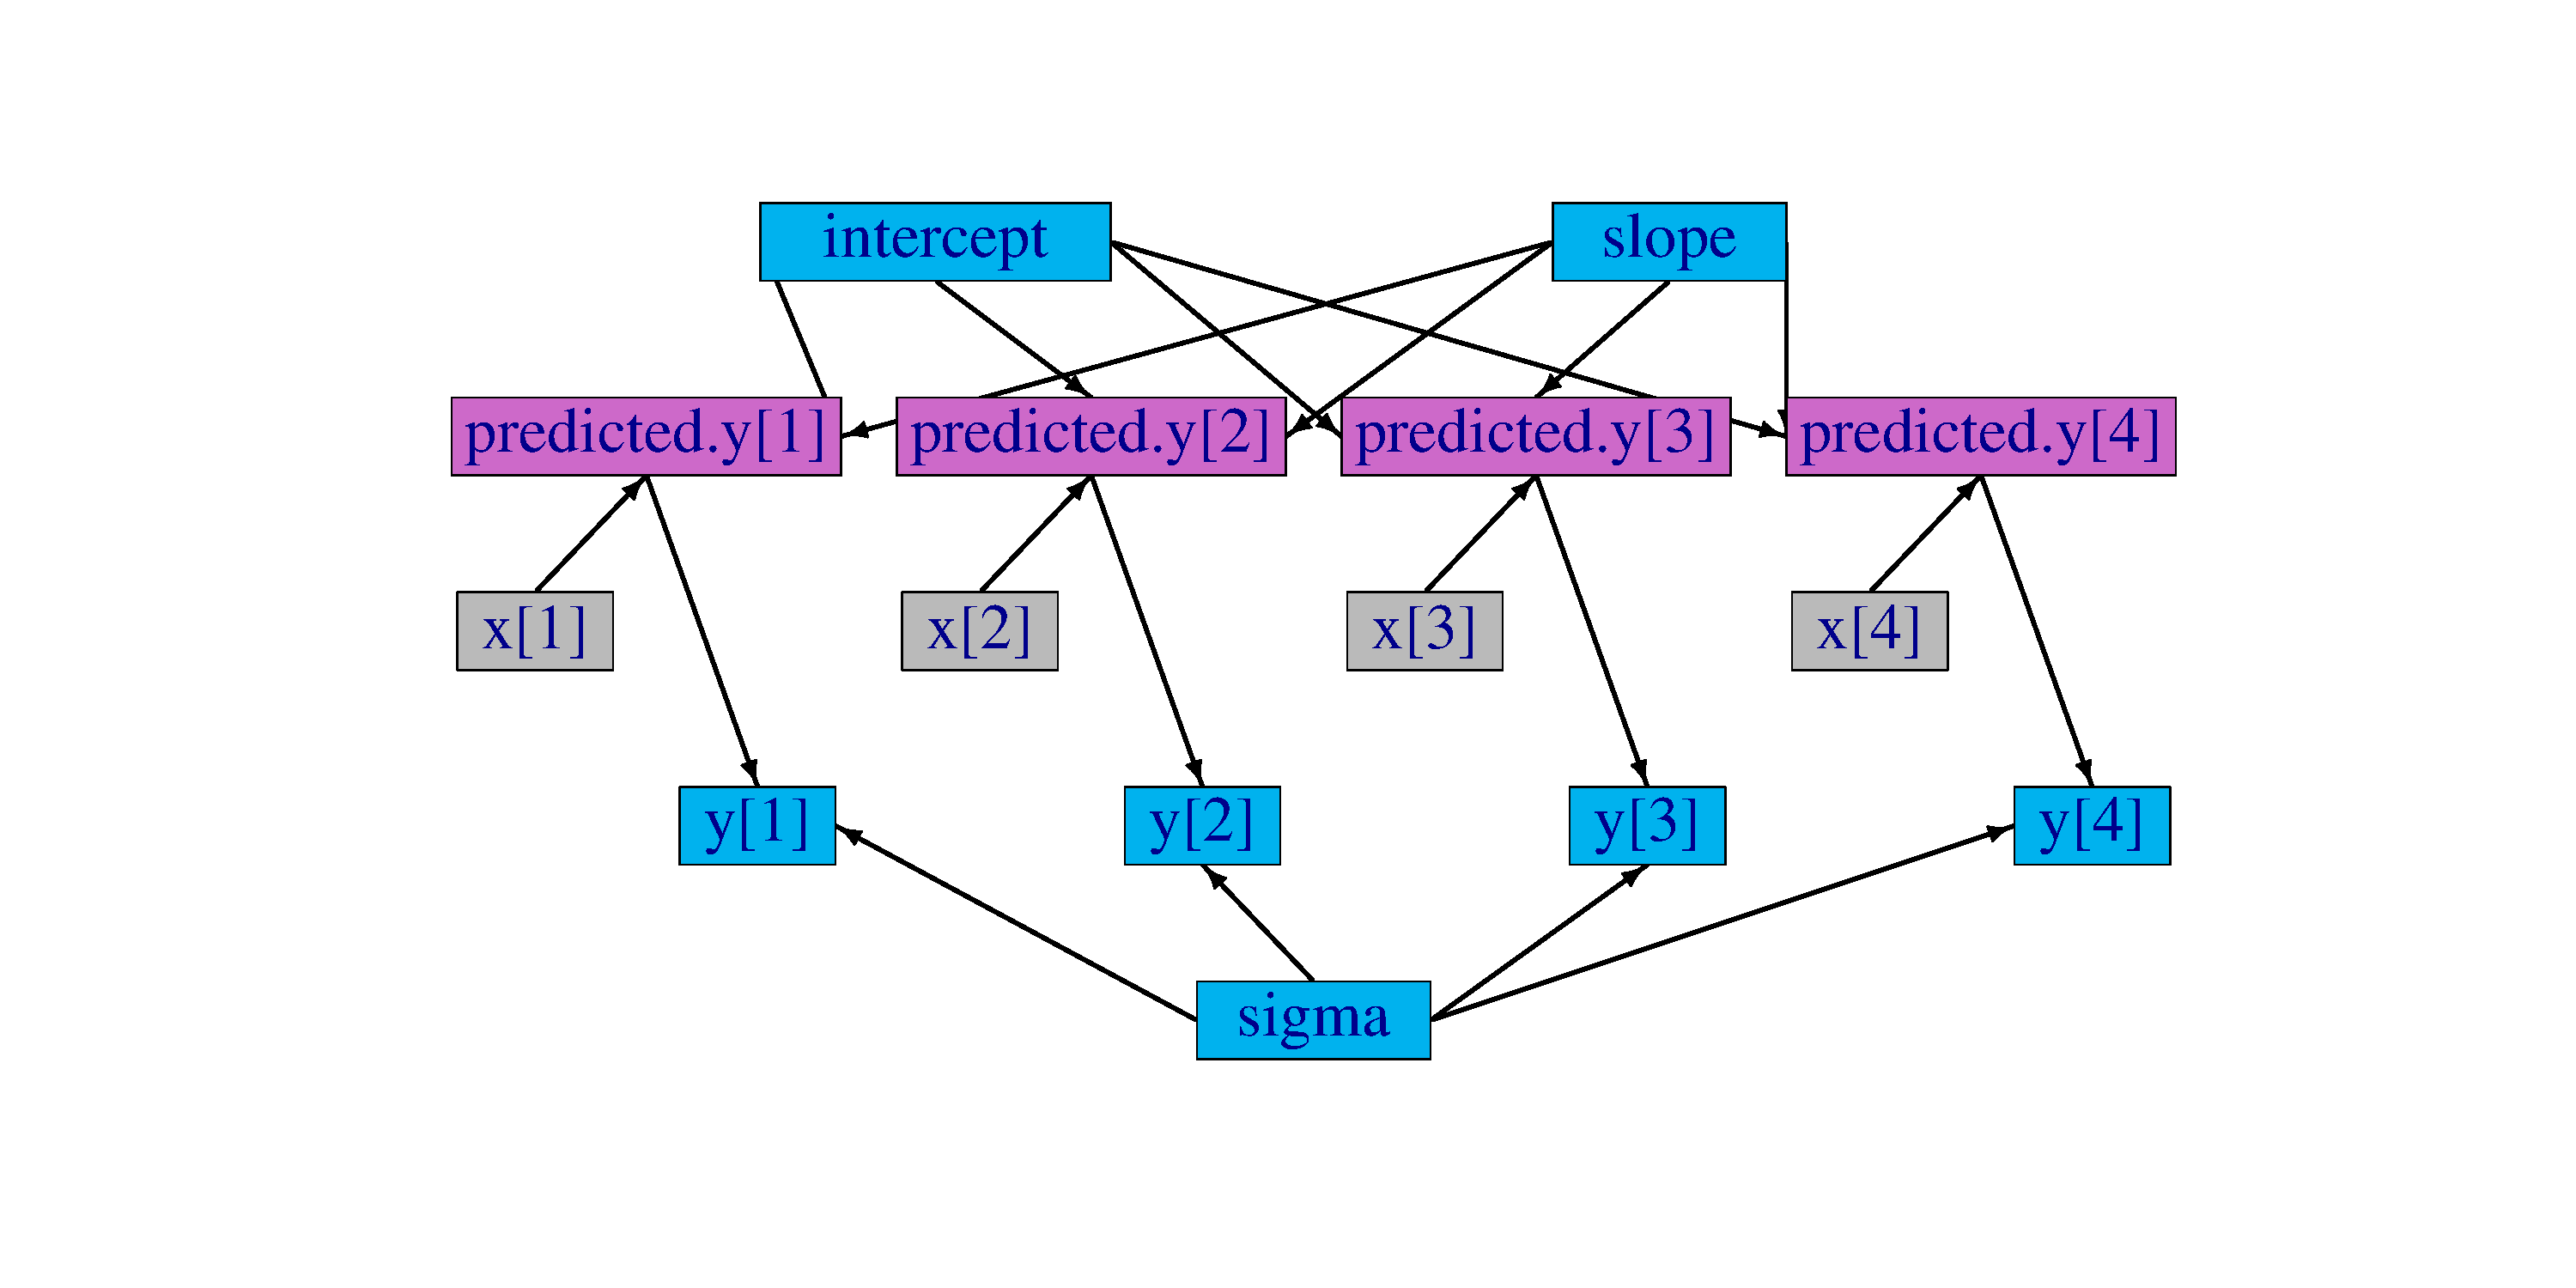
\includegraphics[width=\maxwidth]{figure/linearRegressionGraph-1} \caption[Graph of a linear regression model]{Graph of a linear regression model}\label{fig:linearRegressionGraph}
\end{figure}


\end{knitrout}

The graph representing the model is 
shown in Figure \ref{fig:linearRegressionGraph}.  Each observation,
\cd{y[i]}, is a node whose edges say that it follows a normal
distribution depending on a predicted value, \cd{predicted.y[i]}, and
standard deviation, \cd{sigma}, which are each nodes.  Each predicted
value is a node whose edges say how it is calculated from \cd{slope},
\cd{intercept}, and one value of an explanatory variable, \cd{x[i]},
which are each nodes.

This graph is created from the following BUGS code:

\begin{knitrout}
\definecolor{shadecolor}{rgb}{0.969, 0.969, 0.969}\color{fgcolor}\begin{kframe}
\begin{alltt}
\hlstd{\{}
    \hlstd{intercept} \hlopt{~} \hlkwd{dnorm}\hlstd{(}\hlnum{0}\hlstd{,} \hlkwc{sd} \hlstd{=} \hlnum{1000}\hlstd{)}
    \hlstd{slope} \hlopt{~} \hlkwd{dnorm}\hlstd{(}\hlnum{0}\hlstd{,} \hlkwc{sd} \hlstd{=} \hlnum{1000}\hlstd{)}
    \hlstd{sigma} \hlopt{~} \hlkwd{dunif}\hlstd{(}\hlnum{0}\hlstd{,} \hlnum{100}\hlstd{)}
    \hlkwa{for}\hlstd{(i} \hlkwa{in} \hlnum{1}\hlopt{:}\hlnum{4}\hlstd{) \{}
        \hlstd{predicted.y[i]} \hlkwb{<-} \hlstd{intercept} \hlopt{+} \hlstd{slope} \hlopt{*} \hlstd{x[i]}
        \hlstd{y[i]} \hlopt{~} \hlkwd{dnorm}\hlstd{(predicted.y[i],} \hlkwc{sd} \hlstd{= sigma)}
    \hlstd{\}}
\hlstd{\}}
\end{alltt}
\end{kframe}
\end{knitrout}

In this code, stochastic relationships are declared with ``$\sim$''
and deterministic relationships are declared with ``\cd{<-}''.  For
example, each \cd{y[i]} follows a normal distribution with mean
\cd{predicted.y[i]} and standard deviation
\cd{sigma}.  Each
\cd{predicted.y[i]} is the result of \cd{intercept + slope * x[i]}.
The for-loop yields the equivalent of writing four lines of code, each
with a different value of \cd{i}.  It does not matter in what order
the nodes are declared.  Imagine that each line of code draws part of
Figure \ref{fig:linearRegressionGraph}, and all that matters is that
the everything gets drawn in the end.  Available distributions, default and alternative
  parameterizations, and functions are listed in Section \ref{subsec:dists-and-functions}.

An equivalent graph can be created by this BUGS code:

\begin{knitrout}
\definecolor{shadecolor}{rgb}{0.969, 0.969, 0.969}\color{fgcolor}\begin{kframe}
\begin{alltt}
\hlstd{\{}
    \hlstd{intercept} \hlopt{~} \hlkwd{dnorm}\hlstd{(}\hlnum{0}\hlstd{,} \hlkwc{sd} \hlstd{=} \hlnum{1000}\hlstd{)}
    \hlstd{slope} \hlopt{~} \hlkwd{dnorm}\hlstd{(}\hlnum{0}\hlstd{,} \hlkwc{sd} \hlstd{=} \hlnum{1000}\hlstd{)}
    \hlstd{sigma} \hlopt{~} \hlkwd{dunif}\hlstd{(}\hlnum{0}\hlstd{,} \hlnum{100}\hlstd{)}
    \hlkwa{for}\hlstd{(i} \hlkwa{in} \hlnum{1}\hlopt{:}\hlnum{4}\hlstd{) \{}
        \hlstd{y[i]} \hlopt{~} \hlkwd{dnorm}\hlstd{(intercept} \hlopt{+} \hlstd{slope} \hlopt{*} \hlstd{x[i],} \hlkwc{sd} \hlstd{= sigma)}
    \hlstd{\}}
\hlstd{\}}
\end{alltt}
\end{kframe}
\end{knitrout}

In this case, the \cd{predicted.y[i]} nodes in Figure
\ref{fig:linearRegressionGraph} will be created automatically by
NIMBLE and will have a different name, generated by NIMBLE.

\subsection{More kinds of BUGS declarations}
\label{sec:more-kinds-bugs}

Here are some examples of valid lines of BUGS code.  This code does
not describe a sensible or complete model, and it includes some
arbitrary indices (e.g. \cd{mvx[8:10, i]}) to illustrate flexibility.
Instead the purpose of each line is to illustrate a feature of
NIMBLE's version of BUGS.

\begin{knitrout}
\definecolor{shadecolor}{rgb}{0.969, 0.969, 0.969}\color{fgcolor}\begin{kframe}
\begin{alltt}
\hlstd{\{}
    \hlcom{## 1. normal distribution with BUGS parameter order}
    \hlstd{x} \hlopt{~} \hlkwd{dnorm}\hlstd{(a} \hlopt{+} \hlstd{b} \hlopt{*} \hlstd{c, tau)}
    \hlcom{## 2. normal distribution with a named parameter}
    \hlstd{y} \hlopt{~} \hlkwd{dnorm}\hlstd{(a} \hlopt{+} \hlstd{b} \hlopt{*} \hlstd{c,} \hlkwc{sd} \hlstd{= sigma)}
    \hlcom{## 3. For-loop and nested indexing}
    \hlkwa{for}\hlstd{(i} \hlkwa{in} \hlnum{1}\hlopt{:}\hlstd{N) \{}
        \hlkwa{for}\hlstd{(j} \hlkwa{in} \hlnum{1}\hlopt{:}\hlstd{M[i]) \{}
            \hlstd{z[i,j]} \hlopt{~} \hlkwd{dexp}\hlstd{(r[ blockID[i] ])}
        \hlstd{\}}
    \hlstd{\}}
    \hlcom{## 4. multivariate distribution with arbitrary indexing}
    \hlkwa{for}\hlstd{(i} \hlkwa{in} \hlnum{1}\hlopt{:}\hlnum{3}\hlstd{)}
        \hlstd{mvx[}\hlnum{8}\hlopt{:}\hlnum{10}\hlstd{, i]} \hlopt{~} \hlkwd{dmnorm}\hlstd{(mvMean[}\hlnum{3}\hlopt{:}\hlnum{5}\hlstd{],} \hlkwc{cov} \hlstd{= mvCov[}\hlnum{1}\hlopt{:}\hlnum{3}\hlstd{,} \hlnum{1}\hlopt{:}\hlnum{3}\hlstd{, i])}
    \hlcom{## 5. User-provided distribution}
    \hlstd{w} \hlopt{~} \hlkwd{dMyDistribution}\hlstd{(}\hlkwc{hello} \hlstd{= x,} \hlkwc{world} \hlstd{= y)}
    \hlcom{## 6. Simple deterministic node}
    \hlstd{d1} \hlkwb{<-} \hlstd{a} \hlopt{+} \hlstd{b}
    \hlcom{## 7. Vector deterministic node with matrix multiplication}
    \hlstd{d2[]} \hlkwb{<-} \hlstd{A[ , ]} \hlopt \hlstd{mvMean[}\hlnum{1}\hlopt{:}\hlnum{5}\hlstd{]}
    \hlcom{## 8. Deterministic node with user-provided function}
    \hlstd{d3} \hlkwb{<-} \hlkwd{foo}\hlstd{(x,} \hlkwc{hooray} \hlstd{= y)}
\hlstd{\}}
\end{alltt}
\end{kframe}
\end{knitrout}

When a variable appears only on the right-hand side, it can be provided via \cd{constants} (in which case it can never be changed) or via \cd{data} or \cd{inits}, as discussed in Chapter \ref{cha:building-models}.  

Notes on the comment-numbered lines are:

\begin{enumerate}
\item \cd{x} follows a normal distribution with mean \cd{a + b*c} and precision \cd{tau} (default BUGS second parameter for \cd{dnorm}).
\item \cd{y} follows a normal distribution with the same mean as \cd{x} but a named standard deviation parameter instead of a precision parameter (sd = 1/sqrt(precision)).
\item \cd{z[i, j]} follows an exponential distribution with parameter
  \cd{r[ blockID[i] ]}.  This shows how for-loops can be used for indexing of variables containing
  multiple nodes.  Nested indexing can be used if the nested indices
  (\cd{blockID}) are provided as constants when the model is defined (via \cd{nimbleModel} or \cd{readBUGSmodel}).  Variables that define for-loop indices (\cd{N} and \cd{M}) must also be provided as constants.  
\item The arbitrary block \cd{mvx[8:10, i]} follows a multivariate
  normal distribution, with a named covariance matrix instead of BUGS'
  default of a precision matrix.  As in R, curly braces for for-loop
  contents are only needed if there is more than one line.
\item \cd{w} follows a user-defined distribution. See Chapter \ref{cha:user-defined}.
\item \cd{d1} is a scalar deterministic node that, when calculated, will be
  set to \cd{a + b}.
\item \cd{d2} is a vector deterministic node using matrix
  multiplication in R's syntax.
\item \cd{d3} is a deterministic node using a user-provided
  function.  See Chapter \ref{cha:user-defined}.
\end{enumerate}

\subsubsection{More about indexing}
\label{sec:indexing} 

Examples of allowed indexing include:
\begin{itemize}
\item \verb|x[i]|             \# a single index
\item \verb|x[i:j]|         \# a range of indices
\item \verb|x[i:j,k:l]| \# multiple single indices or ranges for higher-dimensional arrays
\item \verb|x[i:j, ]|     \# blank indices indicating the full range
\item \verb|x[3*i+7]|     \# computed indices
\item \verb|x[(3*i):(5*i+1)]|  \# computed lower and upper ends of an index range
\end{itemize}
 
NIMBLE does not allow multivariate nodes to be used without
square brackets, which is an incompatibility with JAGS.  Therefore a statement like \cd{xbar <- mean(x)} in JAGS must be converted to
\cd{xbar <- mean(x[])} (if \cd{x} is a vector) or \cd{xbar <-
 mean(x[,])} (if \cd{x} is a matrix) for NIMBLE\footnote{In \cd{nimbleFunctions}
  explained in later chapters, square brackets with blank indices are
  not necessary for multivariate objects.}. Section \ref{sec:prov-dimens-via} discusses how to provide NIMBLE with dimensions of \cd{x} when needed.

Generally NIMBLE supports R-like linear algebra expressions and attempts to follow the same rules as R about
dimensions (although in some cases this is not possible).  For
example, \cd{x[1:3] \%*\% y[1:3]} converts \cd{x[1:3]} into a row
vector and thus computes the inner product, which is returned as a $1
\times 1$ matrix (use \cd{inprod} to get it as a scalar, which it typically easier).  Like in R,
a scalar index will result in dropping a dimension unless the argument
\cd{drop=FALSE} is provided.  For example, \cd{mymatrix[i, 1:3]} will
be a vector of length 3, but \cd{mymatrix[i, 1:3, drop=FALSE]} will be
a $1 \times 3$ matrix.  More about indexing and dimensions is
discussed in Section \ref{sec:manag-dimens-sizes}.

\subsection{Vectorized versus scalar declarations}
\label{subsec:vectorized-versus-scalar-declarations}

Suppose you need nodes \cd{logY[i]} that should be the log of the
corresponding \cd{Y[i]}, say for \cd{i} from 1 to 10.  Conventionally
this would be created with a for loop:
\begin{knitrout}
\definecolor{shadecolor}{rgb}{0.969, 0.969, 0.969}\color{fgcolor}\begin{kframe}
\begin{alltt}
\hlstd{\{}
    \hlkwa{for}\hlstd{(i} \hlkwa{in} \hlnum{1}\hlopt{:}\hlnum{10}\hlstd{) \{}
        \hlstd{logY[i]} \hlkwb{<-} \hlkwd{log}\hlstd{(Y[i])}
    \hlstd{\}}
\hlstd{\}}
\end{alltt}
\end{kframe}
\end{knitrout}

Since NIMBLE supports R-like algebraic expressions, an alternative in
NIMBLE's dialect of BUGS is to use a vectorized declaration like this:
\begin{knitrout}
\definecolor{shadecolor}{rgb}{0.969, 0.969, 0.969}\color{fgcolor}\begin{kframe}
\begin{alltt}
\hlstd{\{}
    \hlstd{logY[}\hlnum{1}\hlopt{:}\hlnum{10}\hlstd{]} \hlkwb{<-} \hlkwd{log}\hlstd{(Y[}\hlnum{1}\hlopt{:}\hlnum{10}\hlstd{])}
\hlstd{\}}
\end{alltt}
\end{kframe}
\end{knitrout}


There is an important difference between the models that are created by the
above two methods.  The first creates 10 scalar nodes, \cd{logY[1]}
$,\ldots,$ \cd{logY[10]}.  The second creates one vector node,
\cd{logY[1:10]}.  If each \cd{logY[i]} is used separately by an algorithm, it may be more efficient computationally if they are declared as scalars.  If they are all used together,
it will often make sense to declare them as a vector.


\subsection{Available distributions}
\label{subsec:dists-and-functions}
\subsubsection{Distributions}
\label{subsec:distributions}

NIMBLE supports most of the distributions allowed in BUGS and
JAGS. Table \ref{table:distributions} lists the distributions that are
currently supported, with their default parameterizations, which match
those of BUGS\footnote{Note that the same distributions are available
  for writing \cd{nimbleFunction}s, but in that case the default
  parameterizations and function names match R's when possible. Please
  see Section \ref{sec:nimble-dist-funs} for how to use distributions
  in \cd{nimbleFunctions}.}. NIMBLE also allows one to use alternative
parameterizations for a variety of distributions as described next.
See Section \ref{sec:user-distributions} to learn how to write new distributions using nimbleFunctions.


%\begin{table}[!h]
\begin{center}
    \small
    \LTcapwidth=\textwidth
    \begin{longtable}{llcll}
  \caption[Distributions with default parameter orders. The value of the random variable is denoted by $x$.]{Distributions with their default order of parameters. The value of the random variable is denoted by $x$.}   \label{table:distributions} \\
      \hline
      Name & Usage & Density & Lower & Upper \\
      \hline
      \endhead
     Bernoulli & \verb+dbern(prob = p)+ & 
      \multirow{2}{*}{$p^x (1 - p)^{1 -x}$} & 
      $0$ & $1$ \\
       & $0 < p < 1$ \\
      Beta & \verb+dbeta(shape1 = a, shape2 = b)+ & 
      \multirow{2}{*}{
        $\frac{\textstyle x^{a-1}(1-x)^{b-1}}{\textstyle \beta(a,b)}$
      } & $0$ & $1$ \\
      & $a > 0$, $b > 0$ \\
      Binomial  & \verb+dbin(prob = p, size = n)+ & 
      \multirow{2}{*}{${n \choose x}  p^x (1-p)^{n-x}$}
        & $0$ & $n$ \\
       & $0 < p < 1$, $n \in \mathbb{N}^*$ \\
      Categorical & \verb+dcat(prob = p)+ & \multirow{2}{*}{$\frac{\textstyle p_x}{\textstyle \sum_i p_i}$} & $1$ & $N$ \\
       & $p \in (\mathbb{R}^+)^N$  \\
       Chi-square & \verb+dchisq(df = k)+ & 
      \multirow{2}{*}{
        $\frac{\textstyle x^{\frac{k}{2} - 1} \exp(-x/2)}
        {\textstyle 2^{\frac{k}{2}} \Gamma({\scriptstyle \frac{k}{2}})}$
      } & 0 & \\
      & $k > 0$ \\
%      Double  & \verb+ddexp(mu,tau)+ & 
 %      \multirow{2}{*}{$\tau \exp(-\tau | x-\mu |)/2$} & & \\
 %     exponential & $\tau > 0$ \\
      Dirichlet & \cd{ddirch(alpha = $\alpha$)} & 
      \multirow{2}{*}{$\Gamma(\sum_i \alpha_i) \prod_j 
        \frac{\textstyle x_j^{\alpha_j - 1}}{\textstyle \Gamma(\alpha_j)}$} & 0 &  \\
       & $\alpha_j \geq 0$ \\
      & \\
      Exponential & \cd{dexp(rate = $\lambda$)} & 
      \multirow{2}{*}{$\lambda \exp(-\lambda x)$} & 0 & \\ 
      & $\lambda > 0$ \\
 %     F   & \verb+df(n,m)+ & 
 %     \multirow{2}{*}{
 %       $\textstyle \frac{\Gamma(\frac{n + m}{2})}
 %                        {\Gamma(\frac{n}{2}) \Gamma(\frac{m}{2})}
 %       \left(\frac{n}{m} \right)^{\frac{n}{2}} x^{\frac{n}{2} - 1} 
 %       \left\{1 + \frac{nx}{m} \right\}^{-\frac{(n + m)}{2}}$} & 0 & \\
 %     & $n > 0$, $m > 0$ \\
      Flat & \cd{dflat()} & $\propto 1$ (improper) & & \\
      Gamma       & \cd{dgamma(shape = r, rate = $\lambda$)} & 
      \multirow{2}{*}{
        $\frac{\textstyle \lambda^r x^{r - 1} \exp(-\lambda x)}
        {\textstyle \Gamma(r)}$} & 0 & \\
      & $\lambda > 0$, $r > 0$ \\
 %     Generalized & \verb+dgen.gamma(r,lambda,b)+ &  
 %     \multirow{2}{*}{
 %       $\frac
 %       {\textstyle b \lambda^{b r} x^{b r - 1}  \exp\{-(\lambda x)^{b}\}}
 %       {\textstyle \Gamma(r)}$
 %     } & $0$ & \\
 %     gamma       & $\lambda >0$, $b > 0$, $r > 0$ \\
      Half flat & \cd{dhalfflat()} & $\propto 1$ (improper) & $0$ & \\
      Inverse      & \cd{dinvgamma(shape = r,} & 
      \multirow{2}{*}{
        $\frac{\textstyle \lambda^r x^{-(r + 1)} \exp(-\lambda / x)}
        {\textstyle \Gamma(r)}$} & 0 & \\
      Gamma & \cd{scale = $\lambda$)}, $\lambda > 0$, $r > 0$ \\
      Logistic    & \cd{dlogis(location = $\mu$,}  &
      \multirow{2}{*}{
        $\frac{\textstyle \tau \exp\{(x - \mu) \tau\}}
        {\textstyle  \left[1 + \exp\{(x - \mu) \tau\}\right]^2}$
      } &  & \\
       & \cd{rate = $\tau$)}, $\tau > 0$ \\
      Log-normal  & \cd{dlnorm(meanlog = $\mu$,} & 
      \multirow{2}{*}{
        $\left(\frac{\tau}{2\pi}\right)^{\frac{1}{2}} x^{-1} \exp \left\{-\tau (\log(x) - \mu)^2 / 2 \right\}$} & 0 \\
       & \cd{taulog = $\tau$)}, $\tau > 0$ \\
 %     Noncentral & \verb+dnchisqr(k, delta)+ & 
 %     \multirow{2}{*}{
 %       $\sum_{r=0}^{\infty} 
 %       \frac{ \exp(-\frac{\delta}{2}) (\frac{\delta}{2})^r}{\textstyle r!} \,
 %       \frac{ x^{(k/2 + r - 1)} \exp(-\frac{x}{2})}
 %            { 2^{(k/2 + r)} \Gamma({ \frac{k}{2} + r})}
 %       $
 %     } & 0 & \\
 %     Chi-squre & $k > 0, \delta \geq 0$ \\
      Multinomial  & \cd{dmulti(prob = p, size = n)} & 
      \multirow{2}{*}{$n! \prod_j 
        \frac{\textstyle p_j^{x_j}}{\textstyle x_j!}$} \\
       & $\sum_j x_j = n$ \\
      Multivariate & \cd{dmnorm(mean = $\mu$, prec = $\Lambda$)} &
      \multirow{2}{*}{
        $(2\pi)^{-\frac{d}{2}}|\Lambda|^{\frac{1}{2}} \exp\{-\frac{(x-\mu)^T \Lambda (x-\mu)}{2}\}$} \\
      normal & $\Lambda$ positive definite \\
      Multivariate & \cd{dmvt(mu = $\mu$, prec = $\Lambda$,} &
      \multirow{2}{*}{
        $\frac{\Gamma(\frac{\nu+d}{2})}{\Gamma(\frac{\nu}{2})(\nu\pi)^{d/2}} |\Lambda|^{1/2} 
                (1+\frac{(x-\mu)^T\Lambda(x-\mu)}{\nu})^{-\frac{\nu+d}{2}}$}  \\
      Student t & \cd{df = $\nu$)}, $\Lambda$ positive definite \\
       Negative & \verb+dnegbin(prob = p, size = r)+ &
      \multirow{2}{*}{${x + r -1 \choose x} p^r (1-p)^x$} & 0 & \\
      binomial & $0 < p \leq 1$, $r \geq 0$ \\
     Normal   & \cd{dnorm(mean = $\mu$, tau = $\tau$)} & 
      \multirow{2}{*}{
        $\left(\frac{\tau}{2\pi}\right)^{\frac{1}{2}} \exp\{- \tau (x - \mu)^2 / 2\}$} & & \\
       & $\tau > 0$ \\
 %     Pareto      & \verb+dpar(alpha, c)+ & 
 %     \multirow{2}{*}{
 %       $\alpha c^{\alpha} x^{-(\alpha + 1)}$
 %     } & $c$ & \\
 %     ~ & $\alpha > 0$, $c > 0$ \\
      Poisson & \cd{dpois(lambda = $\lambda$)} & 
      \multirow{2}{*}{$\frac{\textstyle \exp(-\lambda) \lambda^x}{\textstyle x!}$} & 0 & \\
       & $\lambda > 0$ \\
       Student t   & \cd{dt(mu = $\mu$, tau = $\tau$, df = k)} & 
      \multirow{2}{*}{
        $\textstyle \frac{\Gamma(\frac{k+1}{2})}{\Gamma(\frac{k}{2})} 
        \left(\frac{\tau}{k\pi} \right)^{\frac{1}{2}} 
        \left\{1 + \frac{\tau (x - \mu)^2}{k} \right\}^{-\frac{(k+1)}{2}}$} & & \\
       & $\tau > 0$, $k > 0$ \\
      Uniform     & \verb+dunif(min = a, max = b)+ & 
      \multirow{2}{*}{$\frac{\textstyle 1}{\textstyle b - a}$} & $a$ & $b$ \\
       & $a < b$ \\ 
      Weibull     & \cd{dweib(shape = v, lambda = $\lambda$)} & 
      \multirow{2}{*}{$v  \lambda  x^{v - 1} \exp (- \lambda x^v)$} & 0 & \\
       & $v > 0$, $\lambda > 0$ \\
  %    Beta & \verb+dbetabin(a, b, n)+ &
  %   \multirow{2}{*}{
  %      $\textstyle {a+x-1 \choose x} {b+n-x-1 \choose n - x} 
  %                  {a+b+n-1 \choose n}^{-1}$
  %    } & $0$ & $n$ \\
  %    binomial & $a > 0, b > 0, n \in \mathbb{N}^*$ \\
 %     Noncentral & \verb+dhyper(n1,n2,m1,psi)+ &
 %     \multirow{2}{*}{
 %       $\frac{ {n_1 \choose x} {n_2 \choose m_1 - x} \psi^x}
 %             { \sum_i {n_1 \choose i} {n_2 \choose m_1 - i} \psi^i}$
 %     } &
 %     $\scriptstyle \text{max}(0,n_+ - m_1)$ & 
 %     $\scriptstyle \text{min}(n_1,m_1)$ \\
 %     hypergeometric & $0 \leq n_i$, $0 < m_1 \leq n_+$  \\
      Wishart & \cd{dwish(R = R, df = k)} &
      \multirow{2}{*}{
        $\frac{\textstyle |x|^{(k-p-1)/2} |R|^{k/2} \exp\{-\text{tr}(Rx)/2\}}
               {\textstyle 2^{pk/2} \pi^{p(p-1)/4} \prod_{i=1}{p} \Gamma((k+1-i)/2)}$
      } \\
      & $R \; p \times p$ pos. def., $k \geq p$ \\
      Inverse & \cd{dinvwish(S = S, df = k)} &
      \multirow{2}{*}{
        $\frac{\textstyle |x|^{-(k+p+1)/2} |S|^{k/2} \exp\{-\text{tr}(Sx^{-1})/2\}}                           {\textstyle 2^{pk/2} \pi^{p(p-1)/4} \prod_{i=1}{p} \Gamma((k+1-i)/2)}$ } \\
      Wishart & $S \; p \times p$ pos. def., $k \geq p$ \\
 
  %    Multivariate & \verb+x ~ dmt(mu,Omega,k)+ &
  %    \multirow{2}{*}{
  %      $\frac{\textstyle \Gamma \{(k+p)/2\}}{\textstyle \Gamma(k/2) (n\pi)^{p/2}}
  %      |\Omega|^{1/2}
  %      \left\{1 + \frac{1}{k} (x - \mu)^T \Omega (x - \mu) \right\}^{-\frac{(k+p)}{2}}$   } \\
  %    Student t &  $\Omega$ pos. def. & \\

    \end{longtable}
  \end{center}
%\end{table}

%\newpage


\paragraph{Improper distributions}

Note that \cd{dflat} and \cd{dhalfflat} specify improper prior distributions
and should only be used when the posterior distribution of the model is known to be proper.
Also for these distributions, the density function returns the unnormalized density
and the simulation function returns \cd{NaN} so these distributions
are not appropriate for algorithms that need to simulate from the
prior or require proper (normalized) densities.

\subsubsection{Alternative parameterizations for distributions}
\label{subsec:alternative-params}

NIMBLE allows one to specify distributions in model code using a
variety of parameterizations, including the BUGS
parameterizations. Available parameterizations are listed in Table \ref{table:distributions-alternates}.
To understand how NIMBLE handles alternative parameterizations, it is
useful to distinguish three cases, using the \cd{gamma} distribution
as an example:
\begin{enumerate}
\item A \nm{canonical} parameterization is used directly for
  computations\footnote{Usually this is the parameterization in the
  \cd{Rmath} header of R's C implementation of distributions.}.  For
  \cd{gamma}, this is (shape, scale).  
\item The BUGS parameterization is the one defined in the
  original BUGS language. In general this is the parameterization for which conjugate MCMC samplers can be executed most efficiently. For \cd{gamma}, this is (shape, rate). 
\item An \nm{alternative} parameterization is one that must be
  converted into the \nm{canonical} parameterization.  For \cd{gamma},
  NIMBLE provides both (shape, rate) and (mean, sd) parameterization
  and creates nodes to calculate (shape, scale) from either (shape,
  rate) or (mean, sd).  In the case of \cd{gamma}, the BUGS
  parameterization is also an \nm{alternative} parameterization.

\end{enumerate}

Since NIMBLE provides compatibility with existing BUGS and JAGS
code, the order of parameters places the BUGS parameterization
first.  For example, the order of parameters for \cd{dgamma} is \cd{dgamma(shape, rate, scale, mean, sd)}.  Like R, if
parameter names are not given, they are taken in order, so that (shape,
rate) is the default. This happens to  match R's order of parameters,
but it need not.  If names are given, they can be given in any
order.  NIMBLE knows that rate is an alternative to scale and that
(mean, sd) are an alternative to (shape, scale or rate). 

%\begin{table}[!h]
  \begin{center}
    \LTcapwidth=\textwidth
    \begin{longtable}{ll}

  \caption{Distribution parameterizations allowed in NIMBLE. The first
    column indicates the supported parameterizations for
    distributions given in Table \ref{table:distributions}. The second column indicates the
    relationship to the \nm{canonical} parameterization used in
    NIMBLE. } \label{table:distributions-alternates}\\
      \hline
      Parameterization & NIMBLE re-parameterization \\
      \hline \hline
\endhead
   \texttt{dbern(prob)} & \texttt{dbin(size = 1, prob)} \\
      \texttt{dbeta(shape1, shape2)} & canonical \\
      \texttt{dbeta(mean, sd)} & \verb|dbeta(shape1 = mean^2 * (1-mean) / sd^2 - mean,| \\
      & \verb|shape2 = mean * (1 - mean)^2 / sd^2 + mean - 1)| \\
   \texttt{dbin(prob, size)} & canonical \\
         \texttt{dcat(prob)} & canonical \\
         \texttt{dchisq(df)} & canonical \\
         \texttt{ddirch(alpha)} & canonical \\
      \texttt{dexp(rate)} & canonical \\
       \texttt{dexp(scale)} & \texttt{dexp(rate = 1/scale)} \\
     \texttt{dgamma(shape, scale)} & canonical \\
      \texttt{dgamma(shape, rate)} & \verb|dgamma(shape, scale = 1 / rate)| \\
      \texttt{dgamma(mean, sd)} & \verb|dgamma(shape = mean^2/sd^2, scale = sd^2/mean)| \\
      \texttt{dinvgamma(shape, rate)} & canonical \\
     \texttt{dinvgamma(shape, scale)} & \verb|dgamma(shape, rate = 1 / scale)| \\
     \texttt{dlogis(location, scale)} & canonical \\
     \texttt{dlogis(location, rate)} & \verb|dlogis(location, scale = 1 / rate| \\
     \texttt{dlnorm(meanlog, sdlog)} & canonical \\
     \texttt{dlnorm(meanlog, taulog)} & \verb|dlnorm(meanlog, sdlog = 1 / sqrt(taulog)| \\
     \texttt{dlnorm(meanlog, varlog)} & \verb|dlnorm(meanlog, sdlog = sqrt(varlog)| \\
     \texttt{dmulti(prob, size)} & canonical \\
     \texttt{dmnorm(mean, cholesky, } & canonical (precision) \\
       \hspace{5mm}\texttt{prec\_param=1)}          & \\
     \texttt{dmnorm(mean, cholesky, } & canonical (covariance) \\
       \hspace{5mm}\texttt{prec\_param=0)}          & \\
    \texttt{dmnorm(mean, prec)} & \texttt{dmnorm(mean, cholesky = chol(prec), prec\_param=1)} \\
     \texttt{dmnorm(mean, cov)} & \texttt{dmnorm(mean, cholesky = chol(cov), prec\_param=0)} \\
     \texttt{dmvt(mu, cholesky, df, } & canonical (precision/inverse scale) \\
       \hspace{5mm}\texttt{prec\_param=1)}          & \\
     \texttt{dmvt(mu, cholesky, df, } & canonical (scale) \\
       \hspace{5mm}\texttt{prec\_param=0)}          & \\
     \texttt{dmvt(mu, prec, df)} & \texttt{dmvt(mu, cholesky = chol(prec), df, prec\_param=1)} \\
     \texttt{dmvt(mu, scale, df)} & \texttt{dmvt(mu, cholesky = chol(scale), df, prec\_param=0)} \\
   \texttt{dnegbin(prob, size)} & canonical \\
     \texttt{dnorm(mean, sd)} & canonical \\
     \texttt{dnorm(mean, tau)} & \verb|dnorm(mean, sd = 1 / sqrt(var))| \\
     \texttt{dnorm(mean, var)} & \texttt{dnorm(mean, sd = sqrt(var))} \\
     \texttt{dpois(lambda)} & canonical \\
     \texttt{dt(mu, sigma, df)} & canonical \\
    \texttt{dt(mu, tau, df)} & \verb|dt(mu, sigma = 1 / sqrt(tau), df)| \\
    \texttt{dt(mu, sigma2, df)} & \verb|dt(mu, sigma = sqrt(sigma2), df)| \\
   \texttt{dunif(min, max)} & canonical \\
     \texttt{dweib(shape, scale)} & canonical \\
     \texttt{dweib(shape, rate)} & \verb|dweib(shape, scale = 1 / rate)| \\
     \texttt{dweib(shape, lambda)} & \verb|dweib(shape, scale = lambda^(- 1 / shape)| \\
     \texttt{dwish(cholesky, df)} & canonical (scale) \\
       \hspace{5mm}\texttt{scale\_param=1)}          & \\
     \texttt{dwish(cholesky, df)} & canonical (inverse scale) \\
       \hspace{5mm}\texttt{scale\_param=0)}          & \\
     \texttt{dwish(R, df)} & \texttt{dwish(cholesky = chol(R), df, scale\_param = 0)}\\ 
     \texttt{dwish(S, df)} & \texttt{dwish(cholesky = chol(S), df, scale\_param = 1)}\\ 
     \texttt{dinvwish(cholesky, df)} & canonical (scale) \\
       \hspace{5mm}\texttt{scale\_param=1)}          & \\
     \texttt{dinvwish(cholesky, df)} & canonical (inverse scale) \\
       \hspace{5mm}\texttt{scale\_param=0)}          & \\
     \texttt{dinvwish(R, df)} & \texttt{dinvwish(cholesky = chol(R), df, scale\_param = 0)}\\
     \texttt{dinvwish(S, df)} & \texttt{dinvwish(cholesky = chol(S), df, scale\_param = 1)}\\
     \end{longtable}
  \end{center}
%\end{table}


Note that for multivariate normal, multivariate t, Wishart, and Inverse Wishart, the canonical
parameterization uses the Cholesky decomposition of one of the
precision/inverse scale or covariance/scale matrix. For example, for the multivariate normal, if  \cd{prec\_param=TRUE}, the \cd{cholesky} argument is treated as the Cholesky
decomposition of a precision matrix.  Otherwise it is treated as the
Cholesky decomposition of a covariance matrix. 

% In some cases it may be more efficient to use that parameterization
% directly.  % PdV removed this because it is obtuse: In what cases?
% Doesn't lifting of the cholesky computation take care of inefficiency?
% What does "use that parameterization directly" mean, when there is
% no meaning of "indirect" use of a parameterization?  

In addition, NIMBLE supports alternative distribution names, known as aliases, as in JAGS, as specified in Table \ref{table:distributions-aliases}. 


\begin{table}[!h]
  \begin{center}
    \begin{tabular}{lll}
      \hline
      Distribution & Canonical name & Alias \\
      \hline
     Binomial & dbin & dbinom \\
     Chi-square & dchisq & dchisqr \\     
Dirichlet & ddirch & ddirich \\
Multinomial & dmulti & dmultinom \\
Negative binomial & dnegbin & dnbinom  \\
    Weibull & dweib & dweibull \\ 
    Wishart & dwish & dwishart \\
     \hline
    \end{tabular}
  \caption{Distributions with alternative names (aliases).}
    \label{table:distributions-aliases}
  \end{center}
\end{table}

\newpage


%TODO: WHAT IS THE STATUS OF THE NEXT STATEMENT?: I've added inverse gamma in 0.6-4 and will do inverse wishart in 0.6-5. Hopefully will get to some others as well soon-ish - CJP.

We plan to, but do not currently, include the following distributions as part of core NIMBLE: double exponential (Laplace), beta-binomial, Dirichlet-multinomial, F, Pareto, or forms of the multivariate t other than the standard one provided. 
% [F is easy to add as it has R functions]



\subsection{Available BUGS language functions}
\label{subsec:BUGS-lang-fxns}

Tables \ref{table:functions-bugs}-\ref{table:functions-matrix-bugs} show the
available operators and functions. 
% These are also available for \cd{nimbleFunction} programming (see Chapter \ref{cha:progr-with-models}).  In fact, BUGS model nodes are implemented as \cd{nimbleFunction}s that are custom-generated from BUGS declarations, so it would be more correct to say that functions and operators available for \cd{nimbleFunction}s are also available for the model declarations.
Support for more general R expressions
is covered in Chapter \ref{cha:RCfunctions} about programming
with nimbleFunctions. 

For the most part NIMBLE supports the functions used in BUGS and JAGS,
with exceptions indicated in the table.  Additional functions provided
by NIMBLE are also listed. Note that we provide distribution functions
for use in calculations, namely the ``p'', ``q'', and ``d'' functions.
 See Section \ref{sec:nimble-dist-funs} for details on the syntax for using distribution functions as functions in deterministic calculations, as only some parameterizations are allowed and the names of some distributions differ from those used to define stochastic nodes in a model. 

% TODO: CJP moved this material to Chap 9 - that's where it is most relevant 
% so I thought it best to go into the caveats there
%Currently ``r'' functions only return one random
%draw at a time, and the first argument must always be 1.  For
%multivariate distribution functions the \cd{prec\_param} or
%\cd{scale\_param} argument must be provided, indicating when a
%covariance or precision matrix has been given.  In a future release we
%will provide a variety of distribution functions, including density,
%cumulative distribution and quantile functions, using the same syntax
%as \cd{dnorm}, \cd{pnorm}, \cd{qnorm}.  We will also extend the
%alternative parameterizations with named parameters to
%\cd{nimbleFunctions}.

{
\footnotesize 
\LTcapwidth=\textwidth
\begin{longtable}[c]{lllcc}
 \caption{Functions operating on scalars, many of which can operate on
   each element (component-wise) of vectors and matrices. Status
   column indicates if the function is currently provided in
   NIMBLE.}    \label{table:functions-bugs}\\
\hline
 Usage & Description & Comments & Status & Accepts \\
   &  &  &  & vector input  \\
  \hline \hline \\
\endhead
%%%\begin{table}[!h]
%{
%\footnotesize 
%\LTcapwidth=\textwidth
%\begin{longtable}[c]{lllcc}
% \caption{Functions operating on scalars, many of which can operate on
%   each element (component-wise) of vectors and matrices. Status
%   column indicates if the function is currently provided in
%   NIMBLE.}    \label{table:functions}\\
%\hline
%  Usage & Description & Comments & Status & Accepts \\
%   &  &  &  & vector input  \\
%  \hline \hline \\
%\endhead
  \verb+x | y+, \verb|x & y| & logical OR ($|$) and AND(\&) &  & \Checkmark & \Checkmark \\
  \cd{!x} & logical not &  & \Checkmark & \Checkmark \\
  \cd{x > y}, \cd{x >= y}  & greater than (and or equal to) &  & \Checkmark & \Checkmark \\
  \cd{x < y}, \cd{x <= y}  & less than (and or equal to) &  & \Checkmark & \Checkmark \\
  \cd{x != y}, \cd{x == y}  & (not) equals  &  & \Checkmark & \Checkmark \\
  \cd{x + y}, \cd{x - y}, \cd{x * y} & component-wise operators  & mix of scalar and vector ok  & \Checkmark & \Checkmark \\    
  \cd{x / y}, & component-wise division  & vector $x$ and scalar $y$ ok  & \Checkmark & \Checkmark \\    
\verb|x^y|, \cd{pow(x, y)} & power & $x^y$; vector $x$ and scalar $y$ ok & \Checkmark & \Checkmark \\
\cd{x \%\% y} & modulo (remainder) & & \Checkmark & \\
 \cd{min(x1, x2)},  & min. (max.) of two scalars & & \Checkmark &  See \cd{pmin}, \cd{pmax}\\
 \hspace{5mm} \cd{max(x1, x2)} &  & & & \\
 \cd{exp(x)} & exponential &  & \Checkmark & \Checkmark \\
 \cd{log(x)} & natural logarithm &  & \Checkmark & \Checkmark \\
 \cd{sqrt(x)} & square root &  & \Checkmark & \Checkmark \\
 \cd{abs(x)} & absolute value &  & \Checkmark & \Checkmark \\
 \cd{step(x)} & step function at 0 & 0 if $x<0$, 1 if $x>=0$ & \Checkmark & \Checkmark \\
\cd{equals(x, y)}& equality of two scalars & 1 if $x==y$, 0 if $x != y$ & \Checkmark & \\

 \cd{cube(x)} & third power & $x^3$ & \Checkmark & \Checkmark \\
 \cd{sin(x)}, \cd{cos(x)}, \cd{tan(x)} & trigonometric functions  & & \Checkmark & \Checkmark  \\
 \cd{asin(x)}, \cd{acos(x)},  & inverse trigonometric functions & & \Checkmark & \Checkmark \\
 \hspace{5mm} \cd{atan(x)} &  & &  &  \\
 \cd{asinh(x)}, \cd{acosh(x)},  & inv. hyperbolic trig. functions & & \Checkmark & \Checkmark \\
 \hspace{5mm} \cd{atanh(x)} &  & &  &  \\

 \cd{logit(x)} & logit & $\log(x/(1-x))$  & \Checkmark & \Checkmark\\
 \cd{ilogit(x)}, \cd{expit(x)} & inverse logit & $\exp(x) / (1 + \exp(x)) $  & \Checkmark & \Checkmark\\
 \cd{probit(x)} & probit (Gaussian quantile) & $\Phi^{-1}(x)$  & \Checkmark & \Checkmark\\
 \cd{iprobit(x)}, \cd{phi(x)} & inverse probit (Gaussian CDF) & $\Phi(x)$  & \Checkmark & \Checkmark\\
 \cd{cloglog(x)} & complementary log log & $\log(-\log(1-x))$  & \Checkmark & \Checkmark\\
 \cd{icloglog(x)} & inverse complementary log log & $  1 - \exp(-\exp(x)) $ & \Checkmark & \Checkmark\\

 \cd{ceiling(x)} & ceiling function & $\lceil(x)\rceil$  & \Checkmark & \Checkmark \\
 \cd{floor(x)} & floor function & $\lfloor(x)\rfloor$  & \Checkmark & \Checkmark \\
 \cd{round(x)} & round to integer &   & \Checkmark & \Checkmark \\
 \cd{trunc(x)} & truncation to integer &   & \Checkmark & \Checkmark \\
%\newpage
% \cd{gamma(x)} & gamma function & $\Gamma(x)$ [DISABLE!]  & \Checkmark & \Checkmark\\
 \cd{lgamma(x)}, \cd{loggam(x)} & log gamma function & $\log \Gamma(x)$  & \Checkmark & \Checkmark\\
 \cd{log1p(x)} & log of 1 + x & $\log(1+x)$  & \Checkmark & \Checkmark\\
% \cd{factorial(x)} & factorial & $x!$ [DISABLE!]   & \Checkmark & \Checkmark\\
 \cd{lfactorial(x)},  & log factorial & $\log x!$  & \Checkmark & \Checkmark\\
 \hspace{5mm} \cd{logfact(x)} & & & & \\
 \cd{log1p(x)} & log one-plus & $log(x + 1)$ & \Checkmark & \Checkmark \\
 \cd{qDIST(x, PARAMS)} &``q''  distribution functions &  canonical parameterization & \Checkmark & \Checkmark \\
 \cd{pDIST(x, PARAMS)} &``p''  distribution functions &  canonical parameterization & \Checkmark & \Checkmark \\
 \cd{rDIST(1, PARAMS)} & ``r''  distribution functions &  canonical parameterization & \Checkmark & \Checkmark \\
 \cd{dDIST(x, PARAMS)} &``d''  distribution functions &  canonical parameterization & \Checkmark & \Checkmark \\
 \cd{sort(x)}& & & & \\
 \cd{rank(x, s)}& & & & \\
 \cd{ranked(x, s)}& & & & \\
 \cd{order(x)}& & & & \\
%\end{longtable}
%}
%%%\end{table}



\end{longtable}
}

{
\footnotesize
\LTcapwidth=\textwidth

\begin{longtable}[c]{lllc}
 \caption{Functions operating on vectors and matrices. Status column
  indicates if the function is currently provided in
  NIMBLE.} \label{table:functions-matrix-bugs} \\
  \hline
  Usage & Description & Comments & Status   \\
  \hline \hline \\
\endhead
%%%\begin{table}[!h]

%{
%\footnotesize
%\LTcapwidth=\textwidth

%\begin{longtable}[c]{lllc}
% \caption{Functions operating on vectors and matrices. Status column
%  indicates if the function is currently provided in
%  NIMBLE.} \label{table:functions-matrix-dsl} \\
%  \hline
%  Usage & Description & Comments & Status   \\
%  \hline \hline \\
%\endhead
 \cd{inverse(x)}& matrix inverse & $x$ symmetric, positive definite & \Checkmark  \\
 \cd{chol(x)}& matrix Cholesky factorization & $x$ symmetric, positive definite & \Checkmark   \\
 \cd{t(x)}& matrix transpose & $x^\top$ & \Checkmark  \\
 \cd{x\%*\%y}& matrix multiply & $ xy$; $x$, $y$ conformant & \Checkmark  \\
 \cd{inprod(x, y)}& dot product & $x^\top y$; $x$ and $y$ vectors & \Checkmark \\
 \cd{solve(x, y)}& solve system of equations & $x^{-1} y$; $y$ matrix or vector & \Checkmark \\
 \cd{forwardsolve(x, y)}& solve lower-triangular system of equations & $x^{-1} y$; $x$ lower-triangular & \Checkmark \\
 \cd{backsolve(x, y)}& solve upper-triangular system of equations & $x^{-1} y$; $x$ upper-triangular & \Checkmark \\
% \cd{crossprod(x, y)}& crossproduct & $x^\top y$; $x$, $y$ conformant &   \\
% \cd{det(x)}& matrix determinant & $|x|$  [PERHAPS DISABLE THIS!!!] &  \\
 \cd{logdet(x)}& log matrix determinant & $\log|x|$ &  \Checkmark \\
 \cd{asRow(x)}& convert vector \cd{x} to 1-row matrix & sometimes automatic & \Checkmark\\
 \cd{asCol(x)}& convert vector \cd{x} to 1-column matrix & sometimes automatic & \Checkmark\\
 \cd{sum(x)} & sum of elements of \cd{x} &  & \Checkmark \\
 \cd{mean(x)} & mean of elements of \cd{x} & & \Checkmark \\
 \cd{sd(x)}& standard deviation of elements of \cd{x} & &\Checkmark  \\
 \cd{prod(x)} & product of elements of \cd{x} & & \Checkmark \\
 \cd{min(x)}, \cd{max(x)} & min. (max.) of elements of \cd{x} &  & \Checkmark \\
 \cd{pmin(x, y)}, \cd{pmax(x, y)} & vector of mins (maxs) of elements of \cd{x} and \cd{y} &  & \Checkmark \\

 \cd{interp.lin(x, v1, v2)}& linear interpolation & & \\
% \end{longtable}
%}


%%%\end{table}



\cd{eigen(x)\$values}& matrix eigenvalues  & $x$ symmetric & \Checkmark   \\
\cd{eigen(x)\$vectors}& matrix eigenvectors  & $x$ symmetric & \Checkmark   \\
\cd{svd(x)\$d}& matrix singular values  &  & \Checkmark \\
\cd{svd(x)\$u}& matrix left singular vectors  &  & \Checkmark \\
\cd{svd(x)\$v}& matrix right singular vectors  &  & \Checkmark \\
 \end{longtable}
}



% [NOTE: JAGS source package has the Tex files for Martyn's manual, so we can copy the table formatting - s doc/manual/jags\_user\_manual.tex]

See Section \ref{sec:user-functions} to learn how to use nimbleFunctions to write new functions for use in BUGS code.

\subsection{Available link functions}
\label{subsec:BUGS-link}

NIMBLE allows the link functions listed in Table \ref{table:links}.

%\begin{table}[!h]
\begin{center}
\begin{longtable}{llll}
\caption{Link functions \label{table:links}} \\
 \hline
Link function         & Description & Range & Inverse \\
\hline \hline
  \endhead
\verb+cloglog(y) <- x+ & Complementary log log & $0 < y < 1$ & \verb+y <- icloglog(x)+ \\
\verb+log(y) <- x+    & Log           & $0 < y$ &  \verb+y <- exp(x)+ \\
\verb+logit(y) <- x+  & Logit         & $0 < y < 1$ &  \verb+y <- expit(x)+ \\
\verb+probit(y) <- x+ & Probit        & $0 < y < 1$ &  \verb+y <- iprobit(x)+\\
\hline
\end{longtable}
\end{center}
%\end{table}
      
Link functions are specified as functions applied to a node on the
left hand side of a BUGS expression. To handle link functions in
deterministic declarations, NIMBLE converts the declaration into an
equivalent inverse declaration.  For example, \cd{log(y) <- x} is
converted into \cd{y <- exp(x)}.  In other words, the link function is
just a simple variant for conceptual clarity.  

To handle link functions in a stochastic declaration, NIMBLE
does some processing that inserts an additional node into the model.
For example, the declaration \cd{logit(p[i]) $\sim$ dnorm(mu[i],1)}, is equivalent
to the follow two declarations: 
\begin{itemize}
\item \cd{logit\_p[i] $\sim$ dnorm(mu[i], 1)},
\item \cd{p[i] <- expit(logit\_p[i])}
\end{itemize}
where \cd{expit} is the inverse of \cd{logit}.  

Note that NIMBLE does not provide an automatic way of initializing the additional node (\cd{logit\_p[i]} in this case), which is a parent node of the explicit node (\cd{p[i]}), without explicitly referring to the additional node by the name that NIMBLE generates. 

\subsection{Truncation, censoring, and constraints}
\label{subsec:trunc}

NIMBLE provides three ways to declare boundaries on the value of a variable, each for different situations.  We introduce these and comment on their relationships to related features of JAGS and BUGS.  The three methods are:

\subsubsection{Truncation}
Either of the following forms, 
\begin{itemize}
\item \cd{x $\sim$ dnorm(0, sd = 10) T(0, a)}, or
\item \cd{x $\sim$ T(dnorm(0, sd = 10), 0, a)}, 
  \end{itemize}
  declares that \cd{x} follows a normal distribution between 0 and
  \cd{a} (inclusive of 0 and \cd{a}).  Either boundary may be omitted or may be another node, such as \cd{a} in this example.  The first form is compatible with JAGS, but in NIMBLE it can only be used when reading code from a text file.  When writing model code in R, the second version must be used.  

Truncation means the possible values of \cd{x} are limited a priori, hence the probability density of \cd{x} must be normalized\footnote{NIMBLE uses the CDF and inverse CDF (quantile) functions of a distribution to do this; in some cases if one uses truncation to include only the extreme tail of a distribution, numerical difficulties can arise.}.  In this example it would be the normal probability density divided by its integral from 0 to \cd{a}.  Like JAGS, NIMBLE also provides \cd{I} as a synonym for \cd{T} to accommodate older BUGS code, but \cd{T} is preferred because it disambiguates multiple usages of \cd{I} in BUGS.

\subsubsection{Censoring} Censoring refers to the situation where one datum gives the lower or upper bound on an unobserved random variable.  This is common in survival analysis, when for an individual still surviving at the end of a study, the age of death is not known and hence is ``censored'' (right-censoring).  NIMBLE adopts JAGS syntax for censoring, as follows (using right-censoring as an example):
\begin{knitrout}
\definecolor{shadecolor}{rgb}{0.969, 0.969, 0.969}\color{fgcolor}\begin{kframe}
\begin{alltt}
\hlstd{censored[i]} \hlopt{~} \hlkwd{dinterval}\hlstd{(t[i], c[i])}
\hlstd{t[i]} \hlopt{~} \hlkwd{dweib}\hlstd{(r, mu[i])}
\end{alltt}
\end{kframe}
\end{knitrout}
where \cd{censored[i]} should be given as \cd{data} with a value of 1 if
\cd{t[i]} is right-censored (\cd{t[i] $>$ c[i]}) and 0 if it is
observed.  The data vector for \cd{t} should have \cd{NA} (indicating
missing data) for any censored \cd{t[i]} entries. (As a result, these
nodes will be sampled in an MCMC.)  The data vector for \cd{c} should
give the censoring times corresponding to censored entries and a value
below the observed times for uncensored entries (e.g., \cd{0}, assuming \cd{t[i] $>$ 0}). Left-censoring would be specified by setting \cd{censored[i]} to 0 and \cd{t[i]} to \cd{NA}. 
  

The \cd{dinterval} is not really a distribution but rather a trick: in the above example when \cd{censored[i] = 1} it gives a ``probability'' of 1 if \cd{t[i] $>$ c[i]} and 0 otherwise.  This means that \cd{t[i] $\le$ c[i]} is treated as impossible.  More generally than simple right- or left-censoring, \cd{censored[i] $\sim$ dinterval(t[i], c[i, ])} is defined such that for a vector of increasing cutpoints, \cd{c[i, ]}, \cd{t[i]} is enforced to fall within the \cd{censored[i]}-th cutpoint interval.  This is done by setting data \cd{censored[i]} as follows:
\begin{eqnarray}
\mbox{\cd{censored[i] = 0}} & \mbox{if} & \mbox{\cd{t[i] $\le$ c[i, 1]}} \nonumber \\
\mbox{\cd{censored[i] = m}} & \mbox{if} & \mbox{\cd{c[i, m] $<$ t[i] $\le$ c[i, m+1]} for } 1 <= m <= M \nonumber \\
\mbox{\cd{censored[i] = M}} & \mbox{if} & \mbox{\cd{c[i, M] $<$ t[i]}}.\nonumber
\end{eqnarray}
(The \cd{i} index is provided only for consistency with the previous example.)  The most common uses of \cd{dinterval} will be for left- and right-censored data, in which case \cd{c[i,]} will be a single value (and typically given as simply \cd{c[i]}), and for interval-censored data, in which case \cd{c[i,]} will be a vector of two values.  
% TODO: Next line removed by CJP as I thought it was confusing:
% or \cd{x[i] $\sim$ dinterval(c[i], t[i])} with \cd{x[i]} set to 1.
% WHY - our dinterval code treats the 2nd arg as possibly a vector - the above presumably works for scalars but I think it is clearer if we always use the first arg as the data value and the 2nd as the interval points

Nodes following a \cd{dinterval} distribution should normally be set
as \cd{data} with known values. Otherwise, the node may be simulated during initialization in some algorithms (e.g., MCMC) and thereby establish a permanent, perhaps unintended, constraint.  

Censoring differs from truncation because censoring an observation involves bounds on a random variable that could have taken any value, while in truncation we know a priori that a datum could not have occurred outside the truncation range.  


\subsubsection{Constraints and ordering}

NIMBLE provides a more general way to enforce constraints using \cd{dconstraint(cond)}.  For example, we could specify that the sum of \cd{mu1} and \cd{mu2} must be positive like this:
\begin{knitrout}
\definecolor{shadecolor}{rgb}{0.969, 0.969, 0.969}\color{fgcolor}\begin{kframe}
\begin{alltt}
\hlstd{mu1} \hlopt{~} \hlkwd{dnorm}\hlstd{(}\hlnum{0}\hlstd{,} \hlnum{1}\hlstd{)}
\hlstd{mu2} \hlopt{~} \hlkwd{dnorm}\hlstd{(}\hlnum{0}\hlstd{,} \hlnum{1}\hlstd{)}
\hlstd{constraint_data} \hlopt{~} \hlkwd{dconstraint}\hlstd{( mu1} \hlopt{+} \hlstd{mu2} \hlopt{>} \hlnum{0} \hlstd{)}
\end{alltt}
\end{kframe}
\end{knitrout}
with \cd{constraint\_data} set (as \cd{data}) to 1.  This is
equivalent to a half-normal distribution on the half-plane $\mu_1 +
\mu_2 > 0$.  Nodes following \cd{dconstraint} should be provided as data for the same reason of avoiding unintended initialization described above for \cd{dinterval}.

%If one simulates from the model using the \cd{simulate} functions and the condition is not satisfied, then \cd{const} will be 0 and the log probability of \cd{const} (and therefore of the model as whole) will be $-\infty$.

Formally, \cd{dconstraint(cond)} is a probability distribution on $\left\{ 0, 1 \right\}$ such that $P(1) = 1$ if \cd{cond} is \cd{TRUE} and $P(0) = 1$ if \cd{cond} is \cd{FALSE}. 

% TODO: Chris thought this wording is confusing:
%Like \cd{dinterval}, \cd{dconstraint} results in distributions that are not normalized (e.g. for (\cd{mu1}, \cd{mu2})), which makes most sense if the constraint is observed rather than established a priori. 

Of course, in many cases, parameterizing the model so that the
constraints are automatically respected may be a better strategy than
using \cd{dconstraint}.  One should be cautious about constraints that
would make it hard for an MCMC or optimization to move through the
parameter space (such as equality constraints that involve two or more
parameters). For such restrictive constraints, general purpose
algorithms that are not tailored to the constraints may fail or be inefficient. If constraints are used, it will generally be wise to ensure the model is initialized with values that satisfy them.


\paragraph{Ordering}

To specify an ordering of parameters, such as $\alpha_1 <= \alpha_2 <= \alpha_3$ one can use \cd{dconstraint} as follows: 
\begin{knitrout}
\definecolor{shadecolor}{rgb}{0.969, 0.969, 0.969}\color{fgcolor}\begin{kframe}
\begin{alltt}
\hlstd{constraint_data} \hlopt{~} \hlkwd{dconstraint}\hlstd{( alpha1} \hlopt{<=} \hlstd{alpha2} \hlopt{&} \hlstd{alpha2} \hlopt{<=} \hlstd{alpha3 )}
\end{alltt}
\end{kframe}
\end{knitrout}

Note that unlike in BUGS, one cannot specify prior ordering using syntax such as
\begin{verbatim}
alpha[1] ~ dnorm(0, 1) I(, alpha[2])
alpha[2] ~ dnorm(0, 1) I(alpha[1], alpha[3])
alpha[3] ~ dnorm(0, 1) I(alpha[2], )
\end{verbatim}
as this does not represent a directed acyclic graph. 
% TODO: CHRIS, WOULDN'T THIS WORK WITH \cd{alpha[1] $\sim$ dnorm(0, 1)}?  DOES BUGS REALLY ALLOW THIS NON-DAG?
% PERRY, JAGS manual indicates the above is allowed in BUGS. Are you asking if it would work in NIMBLE with alpha1~dnorm(0,1) -- no because alpha2 still depends on alpha3 and vice versa

Also note that specifying prior ordering using \cd{T(,)} can result in possibly unexpected results.  For example:
\begin{verbatim}
alpha1 ~ dnorm(0, 1)
alpha2 ~ dnorm(0, 1) T(alpha1, )
alpha3 ~ dnorm(0, 1) T(alpha2, )
\end{verbatim}
will enforce \cd{alpha1 $\le$ alpha2 $\le$ alpha3}, but it does not treat the three parameters symmetrically.  Instead it puts a marginal prior on \cd{alpha1} that is standard normal and then constrains \cd{alpha2} and \cd{alpha3} to follow truncated normal distributions. This is not equivalent to a symmetric prior on the three \cd{alpha}s that assigns zero probability density when values are not in order.

NIMBLE does not support the JAGS \cd{sort} syntax.




%% See http://yihui.name/knitr/demo/child/ for documentation on the parent/child document system of knitr







\chapter{Building and using models}
\label{cha:building-models}

This chapter explains how to build and manipulate model objects
starting from BUGS code.


\section{Creating model objects}

NIMBLE provides two functions for creating model objects:
\cd{nimbleModel} and \cd{readBUGSmodel}. The first, \cd{nimbleModel},
is more general and was illustrated in Chapter \ref{cha:intro}. The
second, \cd{readBUGSmodel} provides compatibility with BUGS file
formats for models, variables, data, and initial values for MCMC.  

In addition one can create new model objects from existing model objects.

\subsection{Using \cd{nimbleModel} to create a model}

\cd{nimbleModel} processes BUGS code to determine all the nodes,
variables, and their relationships in a model.  Any constants must be
provided at this step.  Data and initial values can optionally be
provided.  BUGS code passed to \cd{nimbleModel} must go through
\cd{nimbleCode}.

We look again at the pump example from the introduction:

\begin{knitrout}
\definecolor{shadecolor}{rgb}{0.969, 0.969, 0.969}\color{fgcolor}\begin{kframe}
\begin{alltt}
\hlstd{pumpCode} \hlkwb{<-} \hlkwd{nimbleCode}\hlstd{(\{}
  \hlkwa{for} \hlstd{(i} \hlkwa{in} \hlnum{1}\hlopt{:}\hlstd{N)\{}
      \hlstd{theta[i]} \hlopt{~} \hlkwd{dgamma}\hlstd{(alpha,beta);}
      \hlstd{lambda[i]} \hlkwb{<-} \hlstd{theta[i]}\hlopt{*}\hlstd{t[i];}
      \hlstd{x[i]} \hlopt{~} \hlkwd{dpois}\hlstd{(lambda[i])}
  \hlstd{\}}
  \hlstd{alpha} \hlopt{~} \hlkwd{dexp}\hlstd{(}\hlnum{1.0}\hlstd{);}
  \hlstd{beta} \hlopt{~} \hlkwd{dgamma}\hlstd{(}\hlnum{0.1}\hlstd{,}\hlnum{1.0}\hlstd{);}
\hlstd{\})}

\hlstd{pumpConsts} \hlkwb{<-} \hlkwd{list}\hlstd{(}\hlkwc{N} \hlstd{=} \hlnum{10}\hlstd{,}
               \hlkwc{t} \hlstd{=} \hlkwd{c}\hlstd{(}\hlnum{94.3}\hlstd{,} \hlnum{15.7}\hlstd{,} \hlnum{62.9}\hlstd{,} \hlnum{126}\hlstd{,} \hlnum{5.24}\hlstd{,}
                 \hlnum{31.4}\hlstd{,} \hlnum{1.05}\hlstd{,} \hlnum{1.05}\hlstd{,} \hlnum{2.1}\hlstd{,} \hlnum{10.5}\hlstd{))}

\hlstd{pumpData} \hlkwb{<-} \hlkwd{list}\hlstd{(}\hlkwc{x} \hlstd{=} \hlkwd{c}\hlstd{(}\hlnum{5}\hlstd{,} \hlnum{1}\hlstd{,} \hlnum{5}\hlstd{,} \hlnum{14}\hlstd{,} \hlnum{3}\hlstd{,} \hlnum{19}\hlstd{,} \hlnum{1}\hlstd{,} \hlnum{1}\hlstd{,} \hlnum{4}\hlstd{,} \hlnum{22}\hlstd{))}

\hlstd{pumpInits} \hlkwb{<-} \hlkwd{list}\hlstd{(}\hlkwc{alpha} \hlstd{=} \hlnum{1}\hlstd{,} \hlkwc{beta} \hlstd{=} \hlnum{1}\hlstd{,}
              \hlkwc{theta} \hlstd{=} \hlkwd{rep}\hlstd{(}\hlnum{0.1}\hlstd{, pumpConsts}\hlopt{$}\hlstd{N))}

\hlstd{pump} \hlkwb{<-} \hlkwd{nimbleModel}\hlstd{(}\hlkwc{code} \hlstd{= pumpCode,} \hlkwc{name} \hlstd{=} \hlstr{"pump"}\hlstd{,} \hlkwc{constants} \hlstd{= pumpConsts,}
                    \hlkwc{data} \hlstd{= pumpData,} \hlkwc{inits} \hlstd{= pumpInits)}
\end{alltt}
\end{kframe}
\end{knitrout}

\subsubsection{Data and constants}
\label{sec:data-constants}

NIMBLE makes a distinction between data and constants:

\begin{itemize}
\item \nm{Constants} can never be changed and must be provided when a
  model is defined.  For example, a vector of known index values, such
  as for block indices, helps define the model graph itself and must
  be provided as constants.  Variables used in the index ranges of
  for-loops must also be provided as constants.
\item \nm{Data} is a label for the role a node plays in the model.
  Nodes marked as data will by default be protected from any functions
  that would simulate over their values (see \cd{simulate} in Chapter
  \ref{cha:using-bugs-models}), but it is possible to over-ride
  that default or to change their values by direct assignment.  This
  allows an algorithm to be applied to many data sets in the same
  model without re-creating the model each time.  It also allows
  simulation of data in a model.  
  % TODO: I don't think this statement is true (i.e., setData()):
  % Data must be provided when an
  %instance of a model is created from the model definition, although
  % they can also be provided earlier when a model is defined.
\end{itemize}

WinBUGS, OpenBUGS and JAGS do not allow data values to be changed or
different nodes to be labeled as data without starting from the
beginning again.  Hence they do not distinguish between constants and
data.  

For compatibility with BUGS and JAGS, NIMBLE allows both to be
provided in the \cd{constants} argument to \cd{nimbleModel}, in
which case NIMBLE handles values for stochastic nodes as data and
everything else as constants.

Values for nodes that appear only on the right-hand side of BUGS
declarations (e.g., covariates/predictors) can be provided as constants or as data or initial values. There is no real difference between providing as data or initial values and the values can be added after building a model via \cd{setInits} or \cd{setData}. 

\subsubsection{Providing data and initial values to an existing model}

Whereas constants must be provided during the call to
\cd{nimbleModel}, data and initial values can be provided later via
the model member functions \cd{setData} and \cd{setInits}. For
example, if \cd{pumpData} is a named list of data values (as above),
then \cd{pump\$setData(pumpData)} sets the named variables to the
values in the list.

\cd{setData} does two things: it sets the values of the data nodes,
and it flags those nodes as containing data.  nimbleFunction
programmers can then use that information to control whether an
algorithm should over-write data or not.  For example, NIMBLE's
\cd{simulate} functions by default do not overwrite data values but
can be told to do so.  Values of data variables can be replaced, and
the indication of which nodes should be treated as data can be reset
by using the \cd{resetData} method, e.g. \cd{pump\$resetData()}.

\subsubsection{Missing data values}

Sometimes one needs a model variable to have a mix of data and
non-data, often due to missing data values.  In NIMBLE, when data
values are provided, any nodes with \cd{NA} values will \nm{not} be
labeled as data.  A node following a multivariate distribution must be either entirely observed or entirely missing.

Here's an example of running an MCMC on the \nm{pump} model, with two
of the observations taken to be missing.  Some of the steps in this
example are documented more below.  NIMBLE's default MCMC
configuration will treat the missing values as unknowns to be sampled,
as can be seen in the MCMC output here.

\begin{knitrout}
\definecolor{shadecolor}{rgb}{0.969, 0.969, 0.969}\color{fgcolor}\begin{kframe}
\begin{alltt}
\hlstd{pumpMiss} \hlkwb{<-} \hlstd{pump}\hlopt{$}\hlkwd{newModel}\hlstd{()}
\hlstd{pumpMiss}\hlopt{$}\hlkwd{resetData}\hlstd{()}
\hlstd{pumpDataNew} \hlkwb{<-} \hlstd{pumpData}
\hlstd{pumpDataNew}\hlopt{$}\hlstd{x[}\hlkwd{c}\hlstd{(}\hlnum{1}\hlstd{,} \hlnum{3}\hlstd{)]} \hlkwb{<-} \hlnum{NA}
\hlstd{pumpMiss}\hlopt{$}\hlkwd{setData}\hlstd{(pumpDataNew)}

\hlstd{pumpMissConf} \hlkwb{<-} \hlkwd{configureMCMC}\hlstd{(pumpMiss)}
\hlstd{pumpMissConf}\hlopt{$}\hlkwd{addMonitors}\hlstd{(}\hlstr{'x'}\hlstd{,} \hlstr{'alpha'}\hlstd{,} \hlstr{'beta'}\hlstd{,} \hlstr{'theta'}\hlstd{)}
\end{alltt}
\begin{verbatim}
## thin = 1: alpha, beta, x, theta
\end{verbatim}
\begin{alltt}
\hlstd{pumpMissMCMC} \hlkwb{<-} \hlkwd{buildMCMC}\hlstd{(pumpMissConf)}
\hlstd{Cobj} \hlkwb{<-} \hlkwd{compileNimble}\hlstd{(pumpMiss, pumpMissMCMC)}

\hlstd{niter} \hlkwb{<-} \hlnum{10}
\hlkwd{set.seed}\hlstd{(}\hlnum{0}\hlstd{)}
\hlstd{Cobj}\hlopt{$}\hlstd{pumpMissMCMC}\hlopt{$}\hlkwd{run}\hlstd{(niter)}
\end{alltt}
\begin{verbatim}
## NULL
\end{verbatim}
\begin{alltt}
\hlstd{samples} \hlkwb{<-} \hlkwd{as.matrix}\hlstd{(Cobj}\hlopt{$}\hlstd{pumpMissMCMC}\hlopt{$}\hlstd{mvSamples)}

\hlstd{samples[}\hlnum{1}\hlopt{:}\hlnum{5}\hlstd{,} \hlnum{13}\hlopt{:}\hlnum{17}\hlstd{]}
\end{alltt}
\begin{verbatim}
##      x[1] x[2] x[3] x[4] x[5]
## [1,]   17    1    2   14    3
## [2,]   11    1    4   14    3
## [3,]   14    1    9   14    3
## [4,]   11    1   24   14    3
## [5,]    9    1   29   14    3
\end{verbatim}
\end{kframe}
\end{knitrout}

Missing values may also occur in explanatory/predictor variables.  Values for
such variables should be passed in via the \cd{data} argument to
\cd{nimbleModel}, with \cd{NA} for the missing values.  In some
contexts, one would want to specify distributions for such explanatory
variables, for example so that an MCMC would impute the missing values.

\subsubsection{Defining alternative models with the same code}
\label{sec:defin-altern-models}

Avoiding code duplication is a basic principle of good programming. In
NIMBLE, one can use definition-time if-then-else statements to create
different models from the same code.  As a simple example, say we have
a linear regression model and want to consider including or omitting
\cd{x[2]} as an explanatory variable:

\begin{knitrout}
\definecolor{shadecolor}{rgb}{0.969, 0.969, 0.969}\color{fgcolor}\begin{kframe}
\begin{alltt}
\hlstd{regressionCode} \hlkwb{<-} \hlkwd{nimbleCode}\hlstd{(\{}
    \hlstd{intercept} \hlopt{~} \hlkwd{dnorm}\hlstd{(}\hlnum{0}\hlstd{,} \hlkwc{sd} \hlstd{=} \hlnum{1000}\hlstd{)}
    \hlstd{slope1} \hlopt{~} \hlkwd{dnorm}\hlstd{(}\hlnum{0}\hlstd{,} \hlkwc{sd} \hlstd{=} \hlnum{1000}\hlstd{)}
    \hlkwa{if}\hlstd{(includeX2) \{}
        \hlstd{slope2} \hlopt{~} \hlkwd{dnorm}\hlstd{(}\hlnum{0}\hlstd{,} \hlkwc{sd} \hlstd{=} \hlnum{1000}\hlstd{)}
        \hlkwa{for}\hlstd{(i} \hlkwa{in} \hlnum{1}\hlopt{:}\hlstd{N)}
            \hlstd{predictedY[i]} \hlkwb{<-} \hlstd{intercept} \hlopt{+} \hlstd{slope1} \hlopt{*} \hlstd{x1[i]} \hlopt{+} \hlstd{slope2} \hlopt{*} \hlstd{x2[i]}
    \hlstd{\}} \hlkwa{else} \hlstd{\{}
        \hlkwa{for}\hlstd{(i} \hlkwa{in} \hlnum{1}\hlopt{:}\hlstd{N) predictedY[i]} \hlkwb{<-} \hlstd{intercept} \hlopt{+} \hlstd{slope1} \hlopt{*} \hlstd{x1[i]}
    \hlstd{\}}
    \hlstd{sigmaY} \hlopt{~} \hlkwd{dunif}\hlstd{(}\hlnum{0}\hlstd{,} \hlnum{100}\hlstd{)}
    \hlkwa{for}\hlstd{(i} \hlkwa{in} \hlnum{1}\hlopt{:}\hlstd{N) Y[i]} \hlopt{~} \hlkwd{dnorm}\hlstd{(predictedY[i], sigmaY)}
\hlstd{\})}

\hlstd{includeX2} \hlkwb{<-} \hlnum{FALSE}
\hlstd{modelWithoutX2} \hlkwb{<-} \hlkwd{nimbleModel}\hlstd{(regressionCode,} \hlkwc{constants} \hlstd{=} \hlkwd{list}\hlstd{(}\hlkwc{N} \hlstd{=} \hlnum{30}\hlstd{),}
                              \hlkwc{check}\hlstd{=}\hlnum{FALSE}\hlstd{)}
\hlstd{modelWithoutX2}\hlopt{$}\hlkwd{getVarNames}\hlstd{()}
\end{alltt}
\begin{verbatim}
## [1] "intercept"                      
## [2] "slope1"                         
## [3] "predictedY"                     
## [4] "sigmaY"                         
## [5] "lifted_d1_over_sqrt_oPsigmaY_cP"
## [6] "Y"                              
## [7] "x1"
\end{verbatim}
\begin{alltt}
\hlstd{includeX2} \hlkwb{<-} \hlnum{TRUE}
\hlstd{modelWithX2} \hlkwb{<-} \hlkwd{nimbleModel}\hlstd{(regressionCode,} \hlkwc{constants} \hlstd{=} \hlkwd{list}\hlstd{(}\hlkwc{N} \hlstd{=} \hlnum{30}\hlstd{),}
                           \hlkwc{check} \hlstd{=} \hlnum{FALSE}\hlstd{)}
\hlstd{modelWithX2}\hlopt{$}\hlkwd{getVarNames}\hlstd{()}
\end{alltt}
\begin{verbatim}
## [1] "intercept"                      
## [2] "slope1"                         
## [3] "slope2"                         
## [4] "predictedY"                     
## [5] "sigmaY"                         
## [6] "lifted_d1_over_sqrt_oPsigmaY_cP"
## [7] "Y"                              
## [8] "x1"                             
## [9] "x2"
\end{verbatim}
\end{kframe}
\end{knitrout}

Whereas the \nm{constants} are a property of the \nm{model definition}
-- since they may help determine the model structure itself --
\nm{data} nodes can be different in different copies of the model
generated from the same \nm{model definition}.   The \cd{setData} and
\cd{setInits} described above can be used for each copy of the model.

\subsubsection{Providing dimensions via \cd{nimbleModel}}
\label{sec:prov-dimens-via}

\cd{nimbleModel} can usually determine the dimensions of every
variable from the declarations in the BUGS code.  However, it is
possible to use a multivariate object only with empty indices
(e.g. \cd{x[,]}), in which case the dimensions must be provided as an
argument to \cd{nimbleModel}.

Here's an example with multivariate nodes.  The first provides indices, so
no \cd{dimensions} argument is needed, while the second omits the
indices and provides a \cd{dimensions} argument instead.

\begin{knitrout}
\definecolor{shadecolor}{rgb}{0.969, 0.969, 0.969}\color{fgcolor}\begin{kframe}
\begin{alltt}
\hlstd{code} \hlkwb{<-} \hlkwd{nimbleCode}\hlstd{(\{}
  \hlstd{y[}\hlnum{1}\hlopt{:}\hlstd{K]} \hlopt{~} \hlkwd{dmulti}\hlstd{(p[}\hlnum{1}\hlopt{:}\hlstd{K], n)}
  \hlstd{p[}\hlnum{1}\hlopt{:}\hlstd{K]} \hlopt{~} \hlkwd{ddirch}\hlstd{(alpha[}\hlnum{1}\hlopt{:}\hlstd{K])}
  \hlkwd{log}\hlstd{(alpha[}\hlnum{1}\hlopt{:}\hlstd{K])} \hlopt{~} \hlkwd{dmnorm}\hlstd{(alpha0[}\hlnum{1}\hlopt{:}\hlstd{K], R[}\hlnum{1}\hlopt{:}\hlstd{K,} \hlnum{1}\hlopt{:}\hlstd{K])}
\hlstd{\})}

\hlstd{K} \hlkwb{<-} \hlnum{5}
\hlstd{model} \hlkwb{<-} \hlkwd{nimbleModel}\hlstd{(code,} \hlkwc{constants} \hlstd{=} \hlkwd{list}\hlstd{(}\hlkwc{n} \hlstd{=} \hlnum{3}\hlstd{,} \hlkwc{K} \hlstd{= K,}
                          \hlkwc{alpha0} \hlstd{=} \hlkwd{rep}\hlstd{(}\hlnum{0}\hlstd{, K),} \hlkwc{R} \hlstd{=} \hlkwd{diag}\hlstd{(K)),}
                     \hlkwc{check} \hlstd{=} \hlnum{FALSE}\hlstd{)}
\end{alltt}
\begin{verbatim}
## Adding alpha0,R as data for building model.
\end{verbatim}
\begin{alltt}
\hlstd{codeAlt} \hlkwb{<-} \hlkwd{nimbleCode}\hlstd{(\{}
  \hlstd{y[]} \hlopt{~} \hlkwd{dmulti}\hlstd{(p[], n)}
  \hlstd{p[]} \hlopt{~} \hlkwd{ddirch}\hlstd{(alpha[])}
  \hlkwd{log}\hlstd{(alpha[])} \hlopt{~} \hlkwd{dmnorm}\hlstd{(alpha0[], R[ , ])}
\hlstd{\})}

\hlstd{model} \hlkwb{<-} \hlkwd{nimbleModel}\hlstd{(codeAlt,} \hlkwc{constants} \hlstd{=} \hlkwd{list}\hlstd{(}\hlkwc{n} \hlstd{=} \hlnum{3}\hlstd{,} \hlkwc{K} \hlstd{= K,}
                          \hlkwc{alpha0} \hlstd{=} \hlkwd{rep}\hlstd{(}\hlnum{0}\hlstd{, K),} \hlkwc{R} \hlstd{=} \hlkwd{diag}\hlstd{(K)),}
                  \hlkwc{dimensions} \hlstd{=} \hlkwd{list}\hlstd{(}\hlkwc{y} \hlstd{= K,} \hlkwc{p} \hlstd{= K,} \hlkwc{alpha} \hlstd{= K),}
                      \hlkwc{check} \hlstd{=} \hlnum{FALSE}\hlstd{)}
\end{alltt}
\begin{verbatim}
## Adding alpha0,R as data for building model.
\end{verbatim}
\end{kframe}
\end{knitrout}

In that example, since \cd{alpha0} and \cd{R} are provided as constants, we don't need to specify their dimensions.

\subsection{Creating a model from standard BUGS and JAGS input files}
\label{sec:readBUGSmodel}

Users with BUGS and JAGS experience may have files set up in standard
formats for use in BUGS and JAGS.  \cd{readBUGSmodel} can
read in the model, data/constant values and initial values in those
formats. It can also take information directly from R objects
somewhat more flexibly than \cd{nimbleModel}, specifically allowing
inputs set up similarly to those for BUGS and JAGS.
In either case, after processing the inputs, it calls \cd{nimbleModel}.
Note that unlike BUGS and JAGS, only a single set of initial values can be
specified in creating a model. Please see \cd{help(readBUGSmodel)} for argument details.  

As an example of using \cd{readBUGSmodel}, let's create a model for the \nm{pump} example from BUGS.
\begin{knitrout}
\definecolor{shadecolor}{rgb}{0.969, 0.969, 0.969}\color{fgcolor}\begin{kframe}
\begin{alltt}
\hlstd{pumpDir} \hlkwb{<-} \hlkwd{system.file}\hlstd{(}\hlstr{'classic-bugs'}\hlstd{,} \hlstr{'vol1'}\hlstd{,} \hlstr{'pump'}\hlstd{,} \hlkwc{package} \hlstd{=} \hlstr{'nimble'}\hlstd{)}
\hlstd{pumpModel} \hlkwb{<-} \hlkwd{readBUGSmodel}\hlstd{(}\hlstr{'pump.bug'}\hlstd{,} \hlkwc{data} \hlstd{=} \hlstr{'pump-data.R'}\hlstd{,}
                           \hlkwc{inits} \hlstd{=} \hlstr{'pump-init.R'}\hlstd{,} \hlkwc{dir} \hlstd{= pumpDir)}
\end{alltt}
\begin{verbatim}
## Detected x as data within 'constants'.
## Adding x as data for building model.
\end{verbatim}
\end{kframe}
\end{knitrout}

Note that \cd{readBUGSmodel} allows one to include \cd{var} and \cd{data} blocks in the model file as in some of the BUGS examples (such as \cd{inhaler}). The \cd{data} block pre-computes constant and data values. Also note that if  \cd{data} and \cd{inits} are provided
as files, the files should contain R code that creates objects
analogous to what would populate the list if a list were provided
instead.  Please see the JAGS manual examples or the
\file{classic\_bugs} directory in the NIMBLE package for example
syntax. 
% PdV - at some point I think there was discussion of code that would appear in a 'data' block being put in the model code directly, but I think this could lead to variable on the LHS twice with <- and ~, so I think I'm not understanding what we want to allow in code defining a model
% I have no recollection of that idea.  Doesn't sound safe. -Perry
NIMBLE by and large does not need the information given in a \cd{var}
block but occasionally this is used to determine dimensionality, such
as in the case of syntax like \cd{xbar <- mean(x[])} where \cd{x} is a variable that appears only on the right-hand side of BUGS expressions.   

Note that NIMBLE does not handle formatting such as in some of the
original BUGS examples in which data was indicated with syntax such as
\cd{data x in `x.txt'}.

\subsection{Making multiple instances from the same model definition}
\label{sub:multiple-instances}
  
Sometimes it is useful to have more than one copy of the same model.
For example, an algorithm (i.e., nimbleFunction) such as an MCMC will be
bound to a particular model before it is run.  A user could build multiple algorithms
to use the same model instance, or they may want each algorithm to
have its own instance of the model.

There are two ways to create new instances of a model, shown in this example:

\begin{knitrout}
\definecolor{shadecolor}{rgb}{0.969, 0.969, 0.969}\color{fgcolor}\begin{kframe}
\begin{alltt}
\hlstd{simpleCode} \hlkwb{<-} \hlkwd{nimbleCode}\hlstd{(\{}
    \hlkwa{for}\hlstd{(i} \hlkwa{in} \hlnum{1}\hlopt{:}\hlstd{N) x[i]} \hlopt{~} \hlkwd{dnorm}\hlstd{(}\hlnum{0}\hlstd{,} \hlnum{1}\hlstd{)}
    \hlstd{\})}

\hlcom{## Return the model definition only, not a built model}
\hlstd{simpleModelDefinition} \hlkwb{<-} \hlkwd{nimbleModel}\hlstd{(simpleCode,} \hlkwc{constants} \hlstd{=} \hlkwd{list}\hlstd{(}\hlkwc{N} \hlstd{=} \hlnum{10}\hlstd{),}
                                     \hlkwc{returnDef} \hlstd{=} \hlnum{TRUE}\hlstd{,} \hlkwc{check} \hlstd{=} \hlnum{FALSE}\hlstd{)}
\hlcom{## Make one instance of the model}
\hlstd{simpleModelCopy1} \hlkwb{<-} \hlstd{simpleModelDefinition}\hlopt{$}\hlkwd{newModel}\hlstd{(}\hlkwc{check} \hlstd{=} \hlnum{FALSE}\hlstd{)}
\hlcom{## Make another instance from the same definition}
\hlstd{simpleModelCopy2} \hlkwb{<-} \hlstd{simpleModelDefinition}\hlopt{$}\hlkwd{newModel}\hlstd{(}\hlkwc{check} \hlstd{=} \hlnum{FALSE}\hlstd{)}
\hlcom{## Ask simpleModelCopy2 for another copy of itself}
\hlstd{simpleModelCopy3} \hlkwb{<-} \hlstd{simpleModelCopy2}\hlopt{$}\hlkwd{newModel}\hlstd{(}\hlkwc{check} \hlstd{=} \hlnum{FALSE}\hlstd{)}
\end{alltt}
\end{kframe}
\end{knitrout}

Each copy of the model can have different nodes flagged as data and
different values in any nodes.  They cannot have different values of
\cd{N} because that is a constant; it must be a constant because
it helps define the model.

\section{NIMBLE models are objects you can query and manipulate}
\label{sec:nodes-and-variables}

NIMBLE models are objects that can be modified and manipulated from R.
In this section we introduce some basic ways to use a model object.
Chapter \ref{cha:using-bugs-models} covers more topics for writing
algorithms that use models.


\subsection{What are variables and nodes?}
\label{sec:what-are-nodes-and-variables}

This section discusses some basic concepts and terminology to
be able to speak about NIMBLE models clearly.

Suppose we have created a model from the following BUGS code.
% This chunk can be modified to jut remove the nimbleModel call.



\begin{knitrout}
\definecolor{shadecolor}{rgb}{0.969, 0.969, 0.969}\color{fgcolor}\begin{kframe}
\begin{alltt}
\hlstd{mc} \hlkwb{<-} \hlkwd{nimbleCode}\hlstd{(\{}
    \hlstd{a} \hlopt{~} \hlkwd{dnorm}\hlstd{(}\hlnum{0}\hlstd{,} \hlnum{0.001}\hlstd{)}
    \hlkwa{for}\hlstd{(i} \hlkwa{in} \hlnum{1}\hlopt{:}\hlnum{5}\hlstd{) \{}
        \hlstd{y[i]} \hlopt{~} \hlkwd{dnorm}\hlstd{(a,} \hlkwc{sd} \hlstd{=} \hlnum{0.1}\hlstd{)}
        \hlkwa{for}\hlstd{(j} \hlkwa{in} \hlnum{1}\hlopt{:}\hlnum{3}\hlstd{)}
            \hlstd{z[i,j]} \hlopt{~} \hlkwd{dnorm}\hlstd{(y[i], tau)}
    \hlstd{\}}
    \hlstd{tau} \hlopt{~} \hlkwd{dunif}\hlstd{(}\hlnum{0}\hlstd{,} \hlnum{20}\hlstd{)}
    \hlstd{y.squared[}\hlnum{1}\hlopt{:}\hlnum{5}\hlstd{]} \hlkwb{<-} \hlstd{y[}\hlnum{1}\hlopt{:}\hlnum{5}\hlstd{]}\hlopt{^}\hlnum{2}
\hlstd{\})}

\hlstd{model} \hlkwb{<-} \hlkwd{nimbleModel}\hlstd{(mc,} \hlkwc{data} \hlstd{=} \hlkwd{list}\hlstd{(}\hlkwc{z} \hlstd{=} \hlkwd{matrix}\hlstd{(}\hlkwd{rnorm}\hlstd{(}\hlnum{15}\hlstd{),} \hlkwc{nrow} \hlstd{=} \hlnum{5}\hlstd{)))}
\end{alltt}
\end{kframe}
\end{knitrout}

In NIMBLE terminology:
\begin{itemize}
\item The \textit{variables} of this model are \cd{a}, \cd{y}, \cd{z},
  and \cd{y.squared}.
\item The \textit{nodes} of this model are \cd{a}, \cd{y[1]} $,\ldots,$
  \cd{y[5]}, \cd{z[1,1]} $,\ldots,$ \cd{z[5, 3]}, and
  \cd{y.squared[1:5]}.  In graph terminology, nodes are vertices in
  the model graph.
\item the \textit{node functions} of this model are
  \verb|a ~ dnorm(0, 0.001)|, \verb|y[i] ~ dnorm(a, 0.1)|,
  \verb|z[i,j] ~ dnorm(y[i], sd = 0.1)|, and
  \verb|y.squared[1:5] <- y[1:5]^2|.  Each node's calculations are
  handled by a node function.  Sometimes the distinction between
  nodes and node functions is important, but when it is not important
  we may refer to both simply as \textit{nodes}.  
\item  The \textit{scalar elements} of this model include all the scalar
  nodes as well as the scalar elements \cd{y.squared[1]} $,\ldots,$
  \cd{y.squared[5]} of the multivariate node \cd{y.squared[1:5]}.
\end{itemize}



\subsection{Determining the nodes and variables in a model}

  
One can determine the variables in a model using \cd{getVarNames} and the  nodes in a model using \cd{getNodeNames}. Optional arguments to \cd{getNodeNames} allow you to select only certain types of nodes, as discussed in Section \ref{sec:get-nodes} and in the R help for \cd{getNodeNames}. 

\begin{knitrout}
\definecolor{shadecolor}{rgb}{0.969, 0.969, 0.969}\color{fgcolor}\begin{kframe}
\begin{alltt}
\hlstd{model}\hlopt{$}\hlkwd{getVarNames}\hlstd{()}
\end{alltt}
\begin{verbatim}
## [1] "a"                            "y"                           
## [3] "lifted_d1_over_sqrt_oPtau_cP" "z"                           
## [5] "tau"                          "y.squared"
\end{verbatim}
\begin{alltt}
\hlstd{model}\hlopt{$}\hlkwd{getNodeNames}\hlstd{()}
\end{alltt}
\begin{verbatim}
##  [1] "a"                           
##  [2] "tau"                         
##  [3] "y[1]"                        
##  [4] "y[2]"                        
##  [5] "y[3]"                        
##  [6] "y[4]"                        
##  [7] "y[5]"                        
##  [8] "lifted_d1_over_sqrt_oPtau_cP"
##  [9] "y.squared[1:5]"              
## [10] "z[1, 1]"                     
## [11] "z[1, 2]"                     
## [12] "z[1, 3]"                     
## [13] "z[2, 1]"                     
## [14] "z[2, 2]"                     
## [15] "z[2, 3]"                     
## [16] "z[3, 1]"                     
## [17] "z[3, 2]"                     
## [18] "z[3, 3]"                     
## [19] "z[4, 1]"                     
## [20] "z[4, 2]"                     
## [21] "z[4, 3]"                     
## [22] "z[5, 1]"                     
## [23] "z[5, 2]"                     
## [24] "z[5, 3]"
\end{verbatim}
\end{kframe}
\end{knitrout}

Note that some of the nodes may be ``lifted'' nodes introduced by
NIMBLE (Section \ref{sec:introduced-nodes}). In this case \cd{lifted\_d1\_over\_sqrt\_oPtau\_cP} (this is a node for the standard deviation of the \cd{z} nodes using NIMBLE's canonical parameterization of the normal distribution) is the only lifted node in the model.

To determine the dependencies of one or more nodes in the model, you can use \cd{getDependencies} as discussed in Section \ref{sec:cdgetdependencies}.


\subsection{Accessing nodes}
\label{sec:accessing-nodes}

Model variables can be accessed and set just as in R using \cd{\$} and
\cd{[[ ]]}.  For example

\begin{knitrout}
\definecolor{shadecolor}{rgb}{0.969, 0.969, 0.969}\color{fgcolor}\begin{kframe}
\begin{alltt}
\hlstd{model}\hlopt{$}\hlstd{a} \hlkwb{<-} \hlnum{5}
\hlstd{model}\hlopt{$}\hlstd{a}
\end{alltt}
\begin{verbatim}
## [1] 5
\end{verbatim}
\begin{alltt}
\hlstd{model[[}\hlstr{"a"}\hlstd{]]}
\end{alltt}
\begin{verbatim}
## [1] 5
\end{verbatim}
\begin{alltt}
\hlstd{model}\hlopt{$}\hlstd{y[}\hlnum{2}\hlopt{:}\hlnum{4}\hlstd{]} \hlkwb{<-} \hlkwd{rnorm}\hlstd{(}\hlnum{3}\hlstd{)}
\hlstd{model}\hlopt{$}\hlstd{y}
\end{alltt}
\begin{verbatim}
## [1]         NA -0.9261095 -0.1771040  0.4020118         NA
\end{verbatim}
\begin{alltt}
\hlstd{model[[}\hlstr{"y"}\hlstd{]][}\hlkwd{c}\hlstd{(}\hlnum{1}\hlstd{,} \hlnum{5}\hlstd{)]} \hlkwb{<-} \hlkwd{rnorm}\hlstd{(}\hlnum{2}\hlstd{)}
\hlstd{model}\hlopt{$}\hlstd{y}
\end{alltt}
\begin{verbatim}
## [1] -0.7317482 -0.9261095 -0.1771040  0.4020118  0.8303732
\end{verbatim}
\begin{alltt}
\hlstd{model}\hlopt{$}\hlstd{z[}\hlnum{1}\hlstd{,]}
\end{alltt}
\begin{verbatim}
## [1] -0.3340008  1.2079084  0.5210227
\end{verbatim}
\end{kframe}
\end{knitrout}


While nodes that are part of a variable can be accessed as above, each
node also has its own name that can be used to access it directly.  For
example, \cd{y[2]} has the name ``y[2]'' and can be accessed by that
name as follows:


\begin{knitrout}
\definecolor{shadecolor}{rgb}{0.969, 0.969, 0.969}\color{fgcolor}\begin{kframe}
\begin{alltt}
\hlstd{model[[}\hlstr{"y[2]"}\hlstd{]]}
\end{alltt}
\begin{verbatim}
## [1] -0.9261095
\end{verbatim}
\begin{alltt}
\hlstd{model[[}\hlstr{"y[2]"}\hlstd{]]} \hlkwb{<-} \hlopt{-}\hlnum{5}
\hlstd{model}\hlopt{$}\hlstd{y}
\end{alltt}
\begin{verbatim}
## [1] -0.7317482 -5.0000000 -0.1771040  0.4020118  0.8303732
\end{verbatim}
\begin{alltt}
\hlstd{model[[}\hlstr{"z[2, 3]"}\hlstd{]]}
\end{alltt}
\begin{verbatim}
## [1] -0.1587546
\end{verbatim}
\begin{alltt}
\hlstd{model[[}\hlstr{"z[2:4, 1:2]"}\hlstd{]][}\hlnum{1}\hlstd{,} \hlnum{2}\hlstd{]}
\end{alltt}
\begin{verbatim}
## [1] -1.231323
\end{verbatim}
\begin{alltt}
\hlstd{model}\hlopt{$}\hlstd{z[}\hlnum{2}\hlstd{,} \hlnum{2}\hlstd{]}
\end{alltt}
\begin{verbatim}
## [1] -1.231323
\end{verbatim}
\end{kframe}
\end{knitrout}

Notice that node names can include index blocks, such as
\cd{model[["z[2:4, 1:2]"]]}, and these are not strictly required to
correspond to actual nodes.  Such blocks can be subsequently
sub-indexed in the regular R manner, such as \cd{model[["z[2:4, 1:2]"]][1, 2]}.

\subsection{How nodes are named}
\label{sec:how-nodes-are}

Every node has a name that is a character string including its
indices, with a space after every comma.  For example, \cd{X[1, 2, 3]}
has the name ``X[1, 2, 3]''.  Nodes following multivariate
distributions have names that include their index blocks.  For
example, a multivariate node for \cd{X[6:10, 3]} has the name ``X[6:10, 3]''.


The definitive source for node names in a model is
\cd{getNodeNames}, described previously.  

In the event you need to ensure that a name is formatted correctly,
you can use the \cd{expandNodeNames} method. For
example, to get the spaces correctly inserted into ``X[1,1:5]'':

\begin{knitrout}
\definecolor{shadecolor}{rgb}{0.969, 0.969, 0.969}\color{fgcolor}\begin{kframe}
\begin{alltt}
\hlstd{multiVarCode} \hlkwb{<-} \hlkwd{nimbleCode}\hlstd{(\{}
    \hlstd{X[}\hlnum{1}\hlstd{,} \hlnum{1}\hlopt{:}\hlnum{5}\hlstd{]} \hlopt{~} \hlkwd{dmnorm}\hlstd{(mu[], cov[,])}
    \hlstd{X[}\hlnum{6}\hlopt{:}\hlnum{10}\hlstd{,} \hlnum{3}\hlstd{]} \hlopt{~} \hlkwd{dmnorm}\hlstd{(mu[], cov[,])}
\hlstd{\})}

\hlstd{multiVarModel} \hlkwb{<-} \hlkwd{nimbleModel}\hlstd{(multiVarCode,} \hlkwc{dimensions} \hlstd{=}
                   \hlkwd{list}\hlstd{(}\hlkwc{mu} \hlstd{=} \hlnum{5}\hlstd{,} \hlkwc{cov} \hlstd{=} \hlkwd{c}\hlstd{(}\hlnum{5}\hlstd{,}\hlnum{5}\hlstd{)),} \hlkwc{calculate} \hlstd{=} \hlnum{FALSE}\hlstd{)}

\hlstd{multiVarModel}\hlopt{$}\hlkwd{expandNodeNames}\hlstd{(}\hlstr{"X[1,1:5]"}\hlstd{)}
\end{alltt}
\begin{verbatim}
## [1] "X[1, 1:5]"
\end{verbatim}
\end{kframe}
\end{knitrout}

Alternatively, for those inclined to R's less commonly used features, a nice trick is
to use its \cd{parse} and \cd{deparse} functions.  
\begin{knitrout}
\definecolor{shadecolor}{rgb}{0.969, 0.969, 0.969}\color{fgcolor}\begin{kframe}
\begin{alltt}
\hlkwd{deparse}\hlstd{(}\hlkwd{parse}\hlstd{(}\hlkwc{text} \hlstd{=} \hlstr{"X[1,1:5]"}\hlstd{,} \hlkwc{keep.source} \hlstd{=} \hlnum{FALSE}\hlstd{)[[}\hlnum{1}\hlstd{]])}
\end{alltt}
\begin{verbatim}
## [1] "X[1, 1:5]"
\end{verbatim}
\end{kframe}
\end{knitrout}


The \cd{keep.source = FALSE} makes \cd{parse} more efficient.

\subsection{Why use node names?}
\label{sec:why-use-node}

Syntax like \cd{model[["z[2, 3]"]]} may seem strange at first, because
the natural habit of an R user would be \cd{model[["z"]][2,3]}.  To see
its utility, consider the example of writing the nimbleFunction given in
Section \ref{sec:creating-your-own}.  By giving every scalar node a name, even
if it is part of a multivariate variable, one can write functions in R
or NIMBLE that access any single node by a name, regardless of the
dimensionality of the variable in which it is embedded.  This is particularly
useful for NIMBLE, which resolves how to access a particular node
during the compilation process.


\subsection{Checking if a node holds data}
\label{sec:cdisdata}

Finally, you can query whether a node is flagged as data using the
\cd{isData} method applied to one or more nodes or nodes within variables:
\begin{knitrout}
\definecolor{shadecolor}{rgb}{0.969, 0.969, 0.969}\color{fgcolor}\begin{kframe}
\begin{alltt}
\hlstd{model}\hlopt{$}\hlkwd{isData}\hlstd{(}\hlstr{'z[1]'}\hlstd{)}
\end{alltt}
\begin{verbatim}
## [1] TRUE
\end{verbatim}
\begin{alltt}
\hlstd{model}\hlopt{$}\hlkwd{isData}\hlstd{(}\hlkwd{c}\hlstd{(}\hlstr{'z[1]'}\hlstd{,} \hlstr{'z[2]'}\hlstd{,} \hlstr{'a'}\hlstd{))}
\end{alltt}
\begin{verbatim}
## [1]  TRUE  TRUE FALSE
\end{verbatim}
\begin{alltt}
\hlstd{model}\hlopt{$}\hlkwd{isData}\hlstd{(}\hlstr{'z'}\hlstd{)}
\end{alltt}
\begin{verbatim}
##  [1] TRUE TRUE TRUE TRUE TRUE TRUE TRUE TRUE TRUE TRUE TRUE TRUE
## [13] TRUE TRUE TRUE
\end{verbatim}
\begin{alltt}
\hlstd{model}\hlopt{$}\hlkwd{isData}\hlstd{(}\hlstr{'z[1:3, 1]'}\hlstd{)}
\end{alltt}
\begin{verbatim}
## [1] TRUE TRUE TRUE
\end{verbatim}
\end{kframe}
\end{knitrout}




\part{Algorithms in NIMBLE}
\label{part:algorithms}






\chapter{MCMC}



Configuring, building and running an MCMC algorithm for a NIMBLE model involves the following steps:

\begin{enumerate}
\item (Optional) Create and customize an MCMC configuration for a particular model:
  \begin{enumerate}
  \item Use \cd{configureMCMC} to create an MCMC configuration (see Section \ref{sec:mcmc-configuration}).  The configuration contains a list of samplers with the node(s) they will sample.
  \item (Optional) Customize the MCMC configuration: 
    \begin{enumerate}
    \item add, remove, or re-order the list of samplers (Section \ref{sec:samplers-provided} and \cd{help(samplers)} in R for details), including adding your own samplers (Section \ref{sec:user-samplers});
    \item change the tuning parameters or adaptive properties of individual samplers;
    \item change the variables to monitor (record for output) and thinning intervals for MCMC samples.
    \end{enumerate}
     
  \end{enumerate}
\item Use \cd{buildMCMC} to build the MCMC object and its samplers either from the model (using default MCMC configuration) or from a customized MCMC configuration (Section \ref{sec:build-compile-mcmc}).
\item Compile the MCMC object (and the model), unless one is debugging and wishes to run the uncompiled MCMC.
\item Run the MCMC and extract the samples (Sections \ref{executing-the-mcmc-algorithm} and \ref{sec:extracting-samples}).
\end{enumerate}

NIMBLE provides several functions to simplify running one or multiple MCMCs:
\begin{itemize}
\item \cd{runMCMC} simplifies the steps of modifying initial values, removing burn-in samples, returning samples in the form of a \cd{coda} \cd{mcmc} object, and running multiple chains for the same MCMC (Section \ref{sec:runMCMC}).
\item \cd{MCMCsuite} can run multiple, different MCMCs for the same model.  These can include multiple NIMBLE MCMCs from different configurations as well as external MCMCs such as from WinBUGS, OpenBUGS, JAGS or Stan (Section \ref{mcmc-suite-compare-mcmcs}).
\item \cd{compareMCMCs} manages multiple calls to \cd{MCMCsuite} and generates html pages comparing performance of different MCMCs.
\end{itemize}

End-to-end examples of MCMC in NIMBLE can be found in Sections \ref{sec:creating-mcmc}-\ref{sec:customizing-mcmc} and Section \ref{sec:mcmc-example-litters}.

% \subsection*{Creating an MCMC algorithm}

% A default MCMC algorithm can be created using \cd{buildMCMC(model)}.  See Section \ref{sec:build-compile-mcmc}.

% To customize properties of the MCMC algorithm -- including the sampling algorithms, joint (block) sampling of dimensions, tuning and adaptive properties of sampling algorithms, variables being monitored (posterior samples are collected), and the thinning interval for sample collection -- an MCMC configuration object (\cd{conf}) must be created using \cd{configureMCMC(model)}.  Properties of the MCMC algorithm can be modified using the \cd{conf} object, after which an MCMC algorithm (\cd{mcmc}) can be created using \cd{buildMCMC(conf)}.  See Section \ref{mcmc-configuration}.

% Both the \cd{model} and \cd{mcmc} should generally be compiled using \cd{compileNimble}, for significantly faster execution (Section \ref{sec:build-compile-mcmc}).  We'll refer to the compiled MCMC algorithm as \cd{Cmcmc}.

% \subsection*{Executing an MCMC algorithm and collecting samples}

% There are two methods available to execute an MCMC algorithm:

% \begin{itemize}
% \item \cd{Cmcmc\$run(...)}
% \item \cd{runMCMC(Cmcmc, ...)}
% \end{itemize}

% Using \cd{Cmcmc\$run(...)} provides lower-level options including extending an MCMC run (collecting additional samples from where it last stopped), and also collecting timing information for the internal sampling algorithms.  After executing an MCMC in this manner, posterior samples are extracted from within the \cd{Cmcmc} object using \cd{as.matrix(Cmcmc\$mvSamples)}.  See Sections \ref{executing-the-mcmc-algorithm} and \ref{sec:extracting-samples}.

% Using \cd{runMCMC(Cmcmc, ...)} provides higher-level options such as running multiple chains, setting initial values, removing burn-in, and returning posterior samples in the form of a \cd{coda} \cd{mcmc} object.  Running an MCMC in this manner returns an array of samples, a list of sample arrays in the case of multiple chains, or optionally a \cd{coda} object.  See Section \ref{sec:runMCMC}.

% \subsection*{Other topics}

% In addition to details of the steps outlined above, this chapter also includes:

% \begin{itemize}
% %%\item NIMBLE's algorithm to search blocks of nodes for efficient joint (block) sampling (section \ref{sec:default-mcmc-conf}) 
% \item Information about the sampling algorithms provided with NIMBLE (Section \ref{sec:samplers-provided})
% \item A detailed example of using the MCMC engine (section \ref{sec:mcmc-example-litters})
% \item Methods to automatically run WinBUGS, OpenBUGS, JAGS, Stan and/or multiple NIMBLE MCMCs on the same model (section \ref{mcmc-suite-compare-mcmcs}) 
% \end{itemize}


\section{The MCMC configuration}
\label{sec:mcmc-configuration}

The MCMC configuration contains information needed for building an MCMC.  When no customization is needed, one can jump directly to the \cd{buildMCMC} step below.  An MCMC configuration is an object of class \cd{MCMCconf}, which includes:

\begin{itemize}
    \item The model on which the MCMC will operate
    \item The model nodes which will be sampled (updated) by the MCMC
    \item The samplers and their internal configurations, called control parameters
    \item Two sets of variables that will be monitored (recorded) during execution of the MCMC and thinning intervals for how often each set will be recorded. Two sets are allowed because it can be useful to monitor different variables at different intervals
\end{itemize}

\subsection{Default MCMC configuration}
\label{sec:default-mcmc-conf}

Assuming we have a model named \cd{Rmodel}, the following will generate a default MCMC configuration:
\begin{knitrout}
\definecolor{shadecolor}{rgb}{0.969, 0.969, 0.969}\color{fgcolor}\begin{kframe}
\begin{alltt}
\hlstd{mcmcConf} \hlkwb{<-} \hlkwd{configureMCMC}\hlstd{(Rmodel)}
\end{alltt}
\end{kframe}
\end{knitrout}

The default configuration will contain a single sampler for each node in the model, and the default ordering follows the topological ordering of the model.

\subsubsection{Default assignment of sampler algorithms}

The default sampler assigned to a stochastic node is determined by the following, in order of precedence:

\begin{enumerate}
\item If the node has no stochastic dependents, a \cd{posterior\_predictive} sampler is assigned.  This sampler sets the new value for the node simply by simulating from its distribution.
\item If the node has a conjugate relationship between its prior distribution and the distributions of its stochastic dependents, a \cd{conjugate} (`Gibbs') sampler is assigned.
\item If the node follows a multinomial distribution, then a \cd{RW\_multinomial} sampler is assigned.  This is a discrete random-walk sampler in the space of multinomial outcomes.
\item If a node follows a Dirichlet distribution, then a \cd{RW\_dirichlet} sampler is assigned.  This is a random walk sampler in the space of the simplex defined by the Dirichlet.
\item If the node follows any other  multivariate distribution, then a \cd{RW\_block} sampler is assigned for all elements.  This is a Metropolis-Hastings adaptive random-walk sampler with a multivariate normal proposal \citep{Roberts_Sahu_1997}.
\item If the node is binary-valued (strictly taking values 0 or 1), then a \cd{binary} sampler is assigned.  This sampler calculates the conditional probability for both possible node values and draws the new node value from the conditional distribution, in effect making a Gibbs sampler.
\item If the node is otherwise discrete-valued, then a \cd{slice} sampler is assigned \citep{Neal2003}.
\item If none of the above criteria are satisfied, then a \cd{RW} sampler is assigned.  This is a Metropolis-Hastings adaptive random-walk sampler with a univariate normal proposal distribution.
\end{enumerate}

These sampler assignment rules can be inspected, reordered, and easily modified using the system option \cd{nimbleOptions("MCMCdefaultSamplerAssignmentRules")}, and customized  \cd{samplerAssignmentRules} objects.

Details of each sampler and its control parameters can be found by invoking \cd{help(samplers)} in R with \cd{nimble} loaded.

\subsubsection{Sampler assignment rules}

The behavior of \cd{configureMCMC} can be customized to control how samplers are assigned.  A new set of sampler assignment rules can be created using \cd{samplerAssignmentRules}, which can be modified using the \cd{addRule} and \cd{reorder} methods, then passed as an argument to \cd{configureMCMC}.  Alternatively, the default behavior of \cd{configureMCMC} can be altered by setting the system option \cd{MCMCdefaultSamplerAssignmentRules} to a custom \cd{samplerAssignmentRules} object.  See \cd{help(samplerAssignmentRules)} for details.

\subsubsection{Options to control default sampler assignments}

As a lightweight alternative to using \cd{samplerAssignmentRules}, very basic control of default sampler assignments is provided via two arguments to \cd{configureMCMC}.  The \cd{useConjugacy} argument controls whether conjugate samplers are assigned when possible, and the \\
\cd{multivariateNodesAsScalars} argument controls whether scalar elements of multivariate nodes are sampled individually. See \cd{help(configureMCMC)} for usage details.

%% The following optional control arguments to \cd{configureMCMC()} may be used to override the default assignment of sampler algorithms:

%% \begin{description}
%% \item[useConjugacy (default \cd{TRUE})] If \cd{TRUE}, conjugate samplers will be assigned to nodes determined to be in conjugate relationships.  If \cd{FALSE}, no conjugate samplers will be assigned.
%% \item[multivariateNodesAsScalars (default \cd{FALSE})]  If \cd{TRUE}, then independent scalar random walk Metropolis-Hastings samplers (\cd{RW}) will be assigned to all scalar components comprising multivariate nodes.  This contrasts the default behavior of a single block sampler being assigned to multivariate nodes.  Regardless of the value of this argument, conjugate samplers will be assigned to conjugate (scalar and multivariate nodes), provided \cd{useConjugacy = TRUE}.
%% \end{description}

\subsubsection{Default monitors}

The default MCMC configuration includes monitors on all top-level stochastic nodes of the model. Only variables that are monitored will have their samples saved for use outside of the MCMC. MCMC configurations include two sets of monitors, each with different thinning intervals.  By default, the second set of monitors (\cd{monitors2}) is empty. 

\subsubsection{Automated parameter blocking}

The default configuration may be replaced by one generated from an automated parameter blocking algorithm.  This algorithm determines groupings of model nodes that, when jointly sampled with a \cd{RW\_block} sampler, increase overall MCMC efficiency.  Overall efficiency is defined as the effective sample size of the slowest-mixing node divided by computation time.  This is done by:

\begin{knitrout}
\definecolor{shadecolor}{rgb}{0.969, 0.969, 0.969}\color{fgcolor}\begin{kframe}
\begin{alltt}
\hlstd{autoBlockConf} \hlkwb{<-} \hlkwd{configureMCMC}\hlstd{(Rmodel,} \hlkwc{autoBlock} \hlstd{=} \hlnum{TRUE}\hlstd{)}
\end{alltt}
\end{kframe}
\end{knitrout}

Note that this using \cd{autoBlock = TRUE} compiles and runs MCMCs, progressively exploring different sampler assignments, so it takes some time and generates some output.  It is most useful for determining effective blocking strategies that can be re-used for later runs.  The additional control argument \cd{autoIt} may also be provided to indicate the number of MCMC samples to be used in each trial of the automated blocking procedure (default 20,000). 

\subsection{Customizing the MCMC configuration}
\label{sec:customizing-mcmc-conf}

The MCMC configuration may be customized in a variety of ways, either through additional named arguments to \cd{configureMCMC} or by calling methods of an existing \cd{MCMCconf} object.

\subsubsection{Controlling which nodes to sample}

One can create an MCMC configuration with default samplers on just a particular set of nodes using the \cd{nodes} argument to \cd{configureMCMC}. The value for the \cd{nodes} argument may be a character vector containing node and/or variable names.  In the case of a variable name, a default sampler will be added for all stochastic nodes in the variable.  The order of samplers will match the order of \cd{nodes}.  Any deterministic nodes will be ignored.

If a data node is included in \cd{nodes}, \emph{it will be assigned a sampler}.  This is the only way in which a default sampler may be placed on a data node and will result in overwriting data values in the node.

\subsubsection{Creating an empty configuration} 
If you plan to customize the choice of all samplers, it can be useful to obtain a configuration with no sampler assignments at all.  This can be done by any of \cd{nodes = NULL}, \cd{nodes = character()}, or \cd{nodes = list()}. 

\subsubsection{Overriding the default sampler assignment rules}
The default rules used for assigning samplers to model nodes can be overridden using the \cd{rules} argument to \cd{configureMCMC}.  This argument must be an object of class \\
\cd{samplerAssignmentRules}, which defines an ordered set of rules for assigning samplers.  Rules can be modified and reordered, to give different precedence to particular samplers, or to assign user-defined samplers (see section \ref{sec:user-samplers}).  The following example creates a new set of rules (which initially contains the default assignment rules), reorders the rules, adds a new rule, then uses these rules to create an MCMC configuration object.

\begin{knitrout}
\definecolor{shadecolor}{rgb}{0.969, 0.969, 0.969}\color{fgcolor}\begin{kframe}
\begin{alltt}
\hlstd{my_rules} \hlkwb{<-} \hlkwd{samplerAssignmentRules}\hlstd{()}
\hlstd{my_rules}\hlopt{$}\hlkwd{reorder}\hlstd{(}\hlkwd{c}\hlstd{(}\hlnum{8}\hlstd{,} \hlnum{1}\hlopt{:}\hlnum{7}\hlstd{))}
\hlstd{my_rules}\hlopt{$}\hlkwd{addRule}\hlstd{(}\hlkwc{condition} \hlstd{=} \hlkwd{quote}\hlstd{(model}\hlopt{$}\hlkwd{getDistribution}\hlstd{(node)} \hlopt{==} \hlstr{"dmnorm"}\hlstd{),}
                 \hlkwc{sampler} \hlstd{= new_dmnorm_sampler)}
\hlstd{mcmcConf} \hlkwb{<-} \hlkwd{configureMCMC}\hlstd{(Rmodel,} \hlkwc{rules} \hlstd{= my_rules)}
\end{alltt}
\end{kframe}
\end{knitrout}

In addition, the default behavior of \cd{configureMCMC} can be altered by setting the system option \cd{nimbleOptions(MCMCdefaultSamplerAssignmentRules = my\_rules)}, or reset to the original default behavior using \cd{nimbleOptions(MCMCdefaultSamplerAssignmentRules = samplerAssignmentRules())}.

\subsubsection{Overriding the default sampler control list values}
The default values of control list elements for all sampling algorithms may be overridden through use of the \cd{control} argument to \cd{configureMCMC}, which should be a named list. 
Named elements in the \cd{control} argument will be used for all default samplers and any subsequent sampler added via \cd{addSampler} (see below).  For example, the following will create the default MCMC configuration, except all \cd{RW} samplers will have their initial \cd{scale} set to 3, and none of the samplers (\cd{RW}, or otherwise) will be adaptive.

\begin{knitrout}
\definecolor{shadecolor}{rgb}{0.969, 0.969, 0.969}\color{fgcolor}\begin{kframe}
\begin{alltt}
\hlstd{mcmcConf} \hlkwb{<-} \hlkwd{configureMCMC}\hlstd{(Rmodel,} \hlkwc{control} \hlstd{=} \hlkwd{list}\hlstd{(}\hlkwc{scale} \hlstd{=} \hlnum{3}\hlstd{,} \hlkwc{adaptive} \hlstd{=} \hlnum{FALSE}\hlstd{))}
\end{alltt}
\end{kframe}
\end{knitrout}

When adding samplers to a configuration using \cd{addSampler}, the default control list can also be over-ridden.

\subsubsection{Adding samplers to the configuration: \cd{addSampler}}

Samplers may be added to a configuration using the \cd{addSampler} method of the \cd{MCMCconf} object.  The first argument gives the node(s) to be sampled, called the \cd{target}, as a character vector.   The second argument gives the type of sampler, which may be provided as a character string or a nimbleFunction object. Valid character strings are indicated in \cd{help(samplers)} (do not include \cd{"sampler\_"}).  Added samplers can be labeled with a \cd{name} argument, which is used in output of \cd{printSamplers}.

Writing a new sampler as a nimbleFunction is covered in Section \ref{sec:user-samplers}.

The hierarchy of precedence for control list elements for samplers is:

\begin{enumerate}
\item The \cd{control} list argument to \cd{addSampler};
\item The \cd{control} list argument to \cd{configureMCMC};
\item The default values, as defined in the sampling algorithm \cd{setup} function.
\end{enumerate}

Samplers added by \cd{addSampler} will be appended to the end of current sampler list.  Adding a sampler for a node will \emph{not} automatically remove any existing samplers on that node. 

\subsubsection{Printing, re-ordering, modifying and removing samplers: \cd{printSamplers},\\\cd{getSamplerDefinition}, and \cd{removeSamplers}}

The current, ordered, list of all samplers in the MCMC configuration may be printed by calling the \cd{printSamplers} method. When you want to see only samplers acting on specific model nodes or variables, provide those names as an argument to \cd{printSamplers}.  The \cd{printSamplers} method accepts arguments controlling the level of detail displayed as discussed in its R help information.

The nimbleFunction definition underlying a particular sampler may be viewed using the \cd{getSamplerDefinition} method, using the sampler index as an argument.  A node name argument may also be supplied, in which case the definition of the first sampler acting on that node is returned.  In all cases, \cd{getSamplerDefinition} only returns the definition of the \emph{first} sampler specified either by index or node name.
\begin{knitrout}
\definecolor{shadecolor}{rgb}{0.969, 0.969, 0.969}\color{fgcolor}\begin{kframe}
\begin{alltt}
\hlcom{## Return the definition of the third sampler in the mcmcConf object}
\hlstd{mcmcConf}\hlopt{$}\hlkwd{getSamplerDefinition}\hlstd{(}\hlnum{3}\hlstd{)}

\hlcom{## Return the definition of the first sampler acting on node "x",}
\hlcom{## or the first of any indexed nodes comprising the variable "x"}
\hlstd{mcmcConf}\hlopt{$}\hlkwd{getSamplerDefinition}\hlstd{(}\hlstr{"x"}\hlstd{)}
\end{alltt}
\end{kframe}
\end{knitrout}

The existing samplers may be re-ordered using the \cd{setSamplers} method. The \cd{ind} argument is a vector of sampler indices, or a character vector of model node or variable names.  Here are a few examples. Each example assumes the \cd{MCMCconf} object initially contains 10 samplers, and each example is independent of the others.
\begin{knitrout}
\definecolor{shadecolor}{rgb}{0.969, 0.969, 0.969}\color{fgcolor}\begin{kframe}
\begin{alltt}
\hlcom{## Truncate the current list of samplers to the first 5}
\hlstd{mcmcConf}\hlopt{$}\hlkwd{setSamplers}\hlstd{(}\hlkwc{ind} \hlstd{=} \hlnum{1}\hlopt{:}\hlnum{5}\hlstd{)}

\hlcom{## Retain only the third sampler, which will subsequently }
\hlcom{## become the first sampler}
\hlstd{mcmcConf}\hlopt{$}\hlkwd{setSamplers}\hlstd{(}\hlkwc{ind} \hlstd{=} \hlnum{3}\hlstd{)}

\hlcom{## Reverse the ordering of the samplers}
\hlstd{mcmcConf}\hlopt{$}\hlkwd{setSamplers}\hlstd{(}\hlkwc{ind} \hlstd{=} \hlnum{10}\hlopt{:}\hlnum{1}\hlstd{)}

\hlcom{## The new set of samplers becomes the }
\hlcom{## \{first, first, first, second, third\} from the current list.}
\hlcom{## Upon each iteration of the MCMC, the 'first' sampler will }
\hlcom{## be executed 3 times, however each instance of the sampler }
\hlcom{## will be independent in terms of scale, adaptation, etc.}
\hlstd{mcmcConf}\hlopt{$}\hlkwd{setSamplers}\hlstd{(}\hlkwc{ind} \hlstd{=} \hlkwd{c}\hlstd{(}\hlnum{1}\hlstd{,} \hlnum{1}\hlstd{,} \hlnum{1}\hlstd{,} \hlnum{2}\hlstd{,} \hlnum{3}\hlstd{))}

\hlcom{## Set the list of samplers to only those acting on model node "alpha"}
\hlstd{mcmcConf}\hlopt{$}\hlkwd{setSamplers}\hlstd{(}\hlstr{"alpha"}\hlstd{)}

\hlcom{## Set the list of samplers to those acting on any components of the}
\hlcom{## model variables "x", "y", or "z".}
\hlstd{mcmcConf}\hlopt{$}\hlkwd{setSamplers}\hlstd{(}\hlkwd{c}\hlstd{(}\hlstr{"x"}\hlstd{,} \hlstr{"y"}\hlstd{,} \hlstr{"z"}\hlstd{))}
\end{alltt}
\end{kframe}
\end{knitrout}

Samplers may be removed from the current sampler ordering with the \cd{removeSamplers} method.  The following examples again assume that \cd{mcmcConf} initially contains 10 samplers, and each example is independent of the others.  \cd{removeSamplers} accepts a vector of numeric indices of samplers to be removed or a character vector.  In the latter case, all samplers acting on the named target model nodes will be removed.
\begin{knitrout}
\definecolor{shadecolor}{rgb}{0.969, 0.969, 0.969}\color{fgcolor}\begin{kframe}
\begin{alltt}
\hlcom{## Remove the first sampler}
\hlstd{mcmcConf}\hlopt{$}\hlkwd{removeSamplers}\hlstd{(}\hlkwc{ind} \hlstd{=} \hlnum{1}\hlstd{)}

\hlcom{## Remove the last five samplers}
\hlstd{mcmcConf}\hlopt{$}\hlkwd{removeSamplers}\hlstd{(}\hlkwc{ind} \hlstd{=} \hlnum{6}\hlopt{:}\hlnum{10}\hlstd{)}

\hlcom{## Remove all samplers,}
\hlcom{## resulting in an empty MCMC configuration, containing no samplers}
\hlstd{mcmcConf}\hlopt{$}\hlkwd{removeSamplers}\hlstd{(}\hlkwc{ind} \hlstd{=} \hlnum{1}\hlopt{:}\hlnum{10}\hlstd{)}

\hlcom{## Remove all samplers acting on "x" or any component of it}
\hlstd{mcmcConf}\hlopt{$}\hlkwd{removeSamplers}\hlstd{(}\hlstr{"x"}\hlstd{)}

\hlcom{## Default: providing no argument removes all samplers}
\hlstd{mcmcConf}\hlopt{$}\hlkwd{removeSamplers}\hlstd{()}
\end{alltt}
\end{kframe}
\end{knitrout}


\subsubsection{Customizing individual sampler configurations: \cd{getSamplers}, \cd{setSamplers}, \cd{setName}, \cd{setSamplerFunction}, \cd{setTarget}, and \cd{setControl}}

Each sampler in an \cd{MCMCconf} object is represented by a sampler configuration as a \cd{samplerConf} object.  Each \cd{samplerConf} is a reference class object containing the following (required) fields: \cd{name} (a character string), \cd{samplerFunction} (a valid nimbleFunction sampler), \cd{target} (the model node to be sampled), and \cd{control} (list of control arguments).  The \cd{MCMCconf} method \cd{getSamplers} allows access to the \cd{samplerConf} objects.  These can be modified and then passed as an argument to \cd{setSamplers} to over-write the current list of samplers in the MCMC configuration object.  However, no checking of the validity of this modified list is performed; if the list of samplerConf objects is corrupted to be invalid, incorrect behavior will result at the time of calling \cd{buildMCMC}.  The fields of a \cd{samplerConf} object can be modified using the access functions \cd{setName(name)}, \cd{setSamplerFunction(fun)}, \cd{setTarget(target, model)}, and \cd{setControl(control)}.

Here are some examples:

\begin{knitrout}
\definecolor{shadecolor}{rgb}{0.969, 0.969, 0.969}\color{fgcolor}\begin{kframe}
\begin{alltt}
\hlcom{## retrieve samplerConf list}
\hlstd{samplerConfList} \hlkwb{<-} \hlstd{mcmcConf}\hlopt{$}\hlkwd{getSamplers}\hlstd{()}

\hlcom{## change the name of the first sampler}
\hlstd{samplerConfList[[}\hlnum{1}\hlstd{]]}\hlopt{$}\hlkwd{setName}\hlstd{(}\hlstr{"newNameForThisSampler"}\hlstd{)}

\hlcom{## change the sampler function of the second sampler,}
\hlcom{## assuming existance of a nimbleFunction 'anotherSamplerNF',}
\hlcom{## which represents a valid nimbleFunction sampler.}
\hlstd{samplerConfList[[}\hlnum{2}\hlstd{]]}\hlopt{$}\hlkwd{setSamplerFunction}\hlstd{(anotherSamplerNF)}

\hlcom{## change the 'adaptive' element of the control list of the third sampler}
\hlstd{control} \hlkwb{<-} \hlstd{samplerConfList[[}\hlnum{3}\hlstd{]]}\hlopt{$}\hlstd{control}
\hlstd{control}\hlopt{$}\hlstd{adaptive} \hlkwb{<-} \hlnum{FALSE}
\hlstd{samplerConfList[[}\hlnum{3}\hlstd{]]}\hlopt{$}\hlkwd{setControl}\hlstd{(control)}

\hlcom{## change the target node of the fourth sampler}
\hlstd{samplerConfList[[}\hlnum{4}\hlstd{]]}\hlopt{$}\hlkwd{setTarget}\hlstd{(}\hlstr{"y"}\hlstd{, model)}   \hlcom{## model argument required}

\hlcom{## use this modified list of samplerConf objects in the MCMC configuration}
\hlstd{mcmcConf}\hlopt{$}\hlkwd{setSamplers}\hlstd{(samplerConfList)}
\end{alltt}
\end{kframe}
\end{knitrout}

\subsubsection{Monitors and thinning intervals: \cd{printMonitors}, \cd{getMonitors}, \cd{addMonitors}, \cd{setThin}, and \cd{resetMonitors}}

An MCMC configuration object contains two independent sets of variables to monitor, each with their own thinning interval: \cd{thin} corresponding to \cd{monitors}, and \cd{thin2} corresponding to \cd{monitors2}.  Monitors operate at the \textit{variable} level.  Only entire model variables may be monitored.  Specifying a monitor on a \textit{node}, e.g., \cd{x[1]}, will result in the entire variable \cd{x} being monitored.

The variables specified in \cd{monitors}  and \cd{monitors2} will be recorded (with thinning interval \cd{thin}) into objects called \cd{mvSamples} and \cd{mvSamples2}, contained within the MCMC object. These are both \nm{modelValues} objects; modelValues are NIMBLE data structures used to store multiple sets of values of model variables\footnote{See Section \ref{sec:modelValues-struct} for general information on modelValues.}.  These can be accessed as the member data \cd{mvSamples} and \cd{mvSamples2} of the MCMC object, and they can be converted to matrices using \cd{as.matrix} (see Section \ref{sec:extracting-samples}).

Monitors may be added to the MCMC configuration either in the original call to \cd{configureMCMC} or using the \cd{addMonitors} method:
\begin{knitrout}
\definecolor{shadecolor}{rgb}{0.969, 0.969, 0.969}\color{fgcolor}\begin{kframe}
\begin{alltt}
\hlcom{## Using an argument to configureMCMC}
\hlstd{mcmcConf} \hlkwb{<-} \hlkwd{configureMCMC}\hlstd{(Rmodel,} \hlkwc{monitors} \hlstd{=} \hlkwd{c}\hlstd{(}\hlstr{"alpha"}\hlstd{,} \hlstr{"beta"}\hlstd{),}
                          \hlkwc{monitors2} \hlstd{=} \hlstr{"x"}\hlstd{)}

\hlcom{## Calling a member method of the mcmcconf object}
\hlcom{## This results in the same monitors as above}
\hlstd{mcmcConf}\hlopt{$}\hlkwd{addMonitors}\hlstd{(}\hlstr{"alpha"}\hlstd{,} \hlstr{"beta"}\hlstd{)}
\hlstd{mcmcConf}\hlopt{$}\hlkwd{addMonitors2}\hlstd{(}\hlstr{"x"}\hlstd{)}
\end{alltt}
\end{kframe}
\end{knitrout}

Similarly, either thinning interval may be set at either step:
\begin{knitrout}
\definecolor{shadecolor}{rgb}{0.969, 0.969, 0.969}\color{fgcolor}\begin{kframe}
\begin{alltt}
\hlcom{## Using an argument to configureMCMC}
\hlstd{mcmcConf} \hlkwb{<-} \hlkwd{configureMCMC}\hlstd{(Rmodel,} \hlkwc{thin} \hlstd{=} \hlnum{1}\hlstd{,} \hlkwc{thin2} \hlstd{=} \hlnum{100}\hlstd{)}

\hlcom{## Calling a member method of the mcmcConf object}
\hlcom{## This results in the same thinning intervals as above}
\hlstd{mcmcConf}\hlopt{$}\hlkwd{setThin}\hlstd{(}\hlnum{1}\hlstd{)}
\hlstd{mcmcConf}\hlopt{$}\hlkwd{setThin2}\hlstd{(}\hlnum{100}\hlstd{)}
\end{alltt}
\end{kframe}
\end{knitrout}

The current lists of monitors and thinning intervals may be displayed using the \cd{printMonitors} method.  Both sets of monitors (\cd{monitors} and \cd{monitors2}) may be reset to empty character vectors by calling the \cd{resetMonitors} method.  The methods \cd{getMonitors}  and \cd{getMonitors2} return the currently specified \cd{monitors} and \cd{monitors2} as character vectors.

\subsubsection{Monitoring model log-probabilities}

To record model log-probabilities from an MCMC, one can add monitors for \emph{logProb} variables (which begin with the prefix \cd{logProb\_}) that correspond to variables with (any) stochastic nodes.   For example, to record and extract log-probabilities for the variables \cd{alpha}, \cd{sigma\_mu}, and \cd{Y}:
\begin{knitrout}
\definecolor{shadecolor}{rgb}{0.969, 0.969, 0.969}\color{fgcolor}\begin{kframe}
\begin{alltt}
\hlstd{mcmcConf} \hlkwb{<-} \hlkwd{configureMCMC}\hlstd{(Rmodel)}
\hlstd{mcmcConf}\hlopt{$}\hlkwd{addMonitors}\hlstd{(}\hlstr{"logProb_alpha"}\hlstd{,} \hlstr{"logProb_sigma_mu"}\hlstd{,} \hlstr{"logProb_Y"}\hlstd{)}
\hlstd{Rmcmc} \hlkwb{<-} \hlkwd{buildMCMC}\hlstd{(mcmcConf)}
\hlstd{Cmodel} \hlkwb{<-} \hlkwd{compileNimble}\hlstd{(Rmodel)}
\hlstd{Cmcmc} \hlkwb{<-} \hlkwd{compileNimble}\hlstd{(Rmcmc,} \hlkwc{project} \hlstd{= Rmodel)}
\hlstd{Cmcmc}\hlopt{$}\hlkwd{run}\hlstd{(}\hlnum{10000}\hlstd{)}
\hlstd{samples} \hlkwb{<-} \hlkwd{as.matrix}\hlstd{(Cmcmc}\hlopt{$}\hlstd{mvSamples)}
\end{alltt}
\end{kframe}
\end{knitrout}

The \cd{samples} matrix will contain both MCMC samples and model log-probabilities.



\section{Building and compiling the MCMC}
\label{sec:build-compile-mcmc}

Once the MCMC configuration object has been created, and customized to one's liking, it may be used to build an MCMC function:

\begin{knitrout}
\definecolor{shadecolor}{rgb}{0.969, 0.969, 0.969}\color{fgcolor}\begin{kframe}
\begin{alltt}
\hlstd{Rmcmc} \hlkwb{<-} \hlkwd{buildMCMC}\hlstd{(mcmcConf)}
\end{alltt}
\end{kframe}
\end{knitrout}

\cd{buildMCMC} is a nimbleFunction.  The returned object \cd{Rmcmc} is an instance  of the nimbleFunction specific to configuration \cd{mcmcConf} (and of course its associated model).

When no customization is needed, one can skip \cd{configureMCMC} and simply provide a model object to \cd{buildMCMC}. The following two MCMC functions will be identical:

\begin{knitrout}
\definecolor{shadecolor}{rgb}{0.969, 0.969, 0.969}\color{fgcolor}\begin{kframe}
\begin{alltt}
\hlstd{mcmcConf} \hlkwb{<-} \hlkwd{configureMCMC}\hlstd{(Rmodel)}   \hlcom{## default MCMC configuration}
\hlstd{Rmcmc1} \hlkwb{<-} \hlkwd{buildMCMC}\hlstd{(mcmcConf)}

\hlstd{Rmcmc2} \hlkwb{<-} \hlkwd{buildMCMC}\hlstd{(Rmodel)}   \hlcom{## uses the default configuration for Rmodel}
\end{alltt}
\end{kframe}
\end{knitrout}

For speed of execution, we usually want to compile the MCMC function to C++ (as is the case for other NIMBLE functions).  To do so, we use \cd{compileNimble}.  If the model has already been compiled, it should be provided as the \cd{project} argument so the MCMC will be part of the same compiled project.  A typical compilation call looks like:

\begin{knitrout}
\definecolor{shadecolor}{rgb}{0.969, 0.969, 0.969}\color{fgcolor}\begin{kframe}
\begin{alltt}
\hlstd{Cmcmc} \hlkwb{<-} \hlkwd{compileNimble}\hlstd{(Rmcmc,} \hlkwc{project} \hlstd{= Rmodel)}
\end{alltt}
\end{kframe}
\end{knitrout}

Alternatively, if the model has not already been compiled, they can be compiled together in one line:

\begin{knitrout}
\definecolor{shadecolor}{rgb}{0.969, 0.969, 0.969}\color{fgcolor}\begin{kframe}
\begin{alltt}
\hlstd{Cmcmc} \hlkwb{<-} \hlkwd{compileNimble}\hlstd{(Rmodel, Rmcmc)}
\end{alltt}
\end{kframe}
\end{knitrout}

Note that if you compile the MCMC with another object (the model in this case), you'll need to explicitly refer to the MCMC component of the resulting object to be able to run the MCMC:

\begin{knitrout}
\definecolor{shadecolor}{rgb}{0.969, 0.969, 0.969}\color{fgcolor}\begin{kframe}
\begin{alltt}
\hlstd{Cmcmc}\hlopt{$}\hlstd{Rmcmc}\hlopt{$}\hlkwd{run}\hlstd{(}\hlkwc{niter} \hlstd{=} \hlnum{1000}\hlstd{)}
\end{alltt}
\end{kframe}
\end{knitrout}


\section{Running the MCMC}
\label{executing-the-mcmc-algorithm}

The MCMC algorithm (either the compiled or uncompiled version) can be executed using the member method \cd{mcmc\$run} (see \cd{help(buildMCMC)} in R).  The \cd{run} method has one required argument, \cd{niter}, the number of iterations to be run.  %Calling \cd{mcmc\$run(niter)} causes the full list of samplers (as determined by the \cd{MCMCconf} object) to be executed \cd{niter} times, and the monitored variables to be stored into the internal \cd{mvSamples} and/or \cd{mvSamples2} objects as governed by the corresponding thinning intervals.

The \cd{run} method has an optional \cd{reset} argument.  When \cd{reset = TRUE} (the default value), the following occurs prior to running the MCMC:
\begin{itemize}
\item All model nodes are checked and filled or updated as needed, in valid (topological) order.  If a stochastic node is missing a value, it is populated using a call to \cd{simulate} and its log probability value is calculated.  The values of deterministic nodes are calculated from their parent nodes.  If any right-hand-side-only nodes (e.g., explanatory variables) are missing a value, an error results.
\item All MCMC sampler functions are reset to their initial state: the initial values of any sampler control parameters (e.g., \cd{scale}, \cd{sliceWidth}, or \cd{propCov}) are reset to their initial values, as were specified by the original MCMC configuration.
\item The internal modelValues objects \cd{mvSamples} and \cd{mvSamples2} are each resized to the appropriate length for holding the requested number of samples (\cd{niter/thin}, and \cd{niter/thin2}, respectively).
\end{itemize}

When \cd{mcmc\$run(niter, reset = FALSE)} is called, the MCMC picks up from where it left off, continuing the previous chain and expanding the output as needed.  No values in the model are checked or altered, and sampler functions are not reset to their initial states.  

The \cd{run} method takes an optional \cd{simulateAll} argument.  When \cd{simulateAll = TRUE}, the \cd{simulate} method of all stochastic nodes is called before running the MCMC.  This generates a new set of initial values.  It should be used with caution since values drawn from priors may be extreme or invalid in some models.

 
\subsection{Measuring sampler computation times: \cd{getTimes}} \label{sec:sampler-time}

If you want to obtain the computation time spent in each sampler, you can set \cd{time=TRUE} as a run-time argument and then use the method \cd{getTimes()} obtain the times.  For example,

\begin{knitrout}
\definecolor{shadecolor}{rgb}{0.969, 0.969, 0.969}\color{fgcolor}\begin{kframe}
\begin{alltt}
\hlstd{Cmcmc}\hlopt{$}\hlkwd{run}\hlstd{(niter,} \hlkwc{time} \hlstd{=} \hlnum{TRUE}\hlstd{)}
\hlstd{Cmcmc}\hlopt{$}\hlkwd{getTimes}\hlstd{()}
\end{alltt}
\end{kframe}
\end{knitrout}
will return a vector of the total time spent in each sampler, measured in seconds. 

\section{Extracting MCMC samples}
\label{sec:extracting-samples}

After executing the MCMC, the output samples can be extracted as follows:

\begin{knitrout}
\definecolor{shadecolor}{rgb}{0.969, 0.969, 0.969}\color{fgcolor}\begin{kframe}
\begin{alltt}
\hlstd{mvSamples} \hlkwb{<-} \hlstd{mcmc}\hlopt{$}\hlstd{mvSamples}
\hlstd{mvSamples2} \hlkwb{<-} \hlstd{mcmc}\hlopt{$}\hlstd{mvSamples2}
\end{alltt}
\end{kframe}
\end{knitrout}

These \nm{modelValues} objects can be converted into matrices using \cd{as.matrix}:

\begin{knitrout}
\definecolor{shadecolor}{rgb}{0.969, 0.969, 0.969}\color{fgcolor}\begin{kframe}
\begin{alltt}
\hlstd{samplesMatrix} \hlkwb{<-} \hlkwd{as.matrix}\hlstd{(mvSamples)}
\hlstd{samplesMatrix2} \hlkwb{<-} \hlkwd{as.matrix}\hlstd{(mvSamples2)}
\end{alltt}
\end{kframe}
\end{knitrout}

The column names of the matrices will be the node names of nodes in the monitored variables.  Then, for example, the mean of the samples for node \cd{x[2]} could be calculated as:

\begin{knitrout}
\definecolor{shadecolor}{rgb}{0.969, 0.969, 0.969}\color{fgcolor}\begin{kframe}
\begin{alltt}
\hlkwd{mean}\hlstd{(samplesMatrix[,} \hlstr{"x[2]"}\hlstd{])}
\end{alltt}
\end{kframe}
\end{knitrout}

Obtaining samples as matrices is most common, but see Section \ref{sec:modelValues-struct} for more about programming with modelValues objects, especially if you want to write nimbleFunctions to use the samples.

\section{Running multiple MCMC chains}
\label{sec:runMCMC}

Once an MCMC algorithm has been created using \cd{buildMCMC}, the function \cd{runMCMC} can be used to run multiple chains and extract samples (see \cd{help(runMCMC)} in R).   \cd{runMCMC} can be used to execute compiled or uncompiled algorithms, although uncompiled algorithms will be much slower.  Specifically, \cd{runMCMC} takes arguments that will control the following aspects of the MCMC:

% \cd{runMCMC} has one mandatory argument: the (compiled or uncompiled) MCMC algorithm.  Other arguments to \cd{runMCMC} are available to control:

\begin{itemize}
\item number of iterations in each chain;
\item number of chains;
\item number of burn-in samples to discard from each chain;
\item initial values, or a function for generating initial values for each chain;
\item setting the random number seed;
\item suppressing messages and output; and
\item returning the samples as a \cd{coda} \cd{mcmc} object.
\end{itemize}

% See \cd{help(runMCMC)} for details of these arguments.

% Other features of the MCMC can still be customized when using \cd{runMCMC}, which is done using the MCMC configuration object.  This includes setting monitors, customizing samplers, or setting a thinning interval (see Section \ref{sec:customizing-mcmc-conf}).  The MCMC configuration object is then used to create an MCMC algorithm, which is compiled and passed as an argument to \cd{runMCMC}.

% When running a single chain, \cd{runMCMC} returns a matrix of MCMC samples (as described in Section \ref{sec:extracting-samples}).  When running multiple chains, a list of sample matrices is returned.  Using the argument \cd{returnCodaMCMC=TRUE}, a \cd{coda} \cd{mcmc} object, or in the case of multiple chains, a \cd{coda} \cd{mcmc.list} object is returned instead.

The following examples demonstrate some uses of \cd{runMCMC}, and assume the existence of \cd{Cmcmc}, a compiled MCMC algorithm.

\begin{knitrout}
\definecolor{shadecolor}{rgb}{0.969, 0.969, 0.969}\color{fgcolor}\begin{kframe}
\begin{alltt}
\hlcom{## run a single chain, return a matrix of samples}
\hlstd{samplesMatrix} \hlkwb{<-} \hlkwd{runMCMC}\hlstd{(Cmcmc)}

\hlcom{## run three chains of 10,000 samples, discard a burn-in of 1,000,}
\hlcom{## and return of list of sample matrices}
\hlstd{samplesList} \hlkwb{<-} \hlkwd{runMCMC}\hlstd{(Cmcmc,} \hlkwc{niter} \hlstd{=} \hlnum{10000}\hlstd{,} \hlkwc{nburnin} \hlstd{=} \hlnum{1000}\hlstd{,} \hlkwc{nchains} \hlstd{=} \hlnum{3}\hlstd{)}

\hlcom{## run two chains, and provide initial values for each}
\hlstd{initsList} \hlkwb{<-} \hlkwd{list}\hlstd{(}\hlkwd{list}\hlstd{(}\hlkwc{mu} \hlstd{=} \hlnum{1}\hlstd{,} \hlkwc{sigma} \hlstd{=} \hlnum{1}\hlstd{),}
                  \hlkwd{list}\hlstd{(}\hlkwc{mu} \hlstd{=} \hlnum{2}\hlstd{,} \hlkwc{sigma} \hlstd{=} \hlnum{10}\hlstd{))}
\hlstd{samplesList} \hlkwb{<-} \hlkwd{runMCMC}\hlstd{(Cmcmc,} \hlkwc{nchains} \hlstd{=} \hlnum{2}\hlstd{,} \hlkwc{inits} \hlstd{= initsList)}

\hlcom{## run ten chains of 100,000 iterations,}
\hlcom{## using a function to generate initial values}
\hlstd{initsFunction} \hlkwb{<-} \hlkwa{function}\hlstd{()}
    \hlkwd{list}\hlstd{(}\hlkwc{mu} \hlstd{=} \hlkwd{rnorm}\hlstd{(}\hlnum{1}\hlstd{,}\hlnum{0}\hlstd{,}\hlnum{1}\hlstd{),} \hlkwc{sigma} \hlstd{=} \hlkwd{runif}\hlstd{(}\hlnum{1}\hlstd{,}\hlnum{0}\hlstd{,}\hlnum{100}\hlstd{))}
\hlstd{samplesList} \hlkwb{<-} \hlkwd{runMCMC}\hlstd{(Cmcmc,} \hlkwc{niter} \hlstd{=} \hlnum{100000}\hlstd{,} \hlkwc{nchains} \hlstd{=} \hlnum{10}\hlstd{,}
                       \hlkwc{inits} \hlstd{= initsFunction)}

\hlcom{## run three chains, using a fixed random number seed for each chain}
\hlstd{samplesList} \hlkwb{<-} \hlkwd{runMCMC}\hlstd{(Cmcmc,} \hlkwc{nchains} \hlstd{=} \hlnum{3}\hlstd{,} \hlkwc{setSeed} \hlstd{=} \hlnum{TRUE}\hlstd{)}

\hlcom{## run three chains, return a coda mcmc.list object}
\hlstd{codaMCMClist} \hlkwb{<-} \hlkwd{runMCMC}\hlstd{(Cmcmc,} \hlkwc{nchains} \hlstd{=} \hlnum{3}\hlstd{,} \hlkwc{returnCodaMCMC} \hlstd{=} \hlnum{TRUE}\hlstd{)}
\end{alltt}
\end{kframe}
\end{knitrout}



\section{Samplers provided with NIMBLE}
\label{sec:samplers-provided}

Most documentation of MCMC samplers provided with NIMBLE can be found by invoking \cd{help(samplers)} in R.  Here we provide additional explanation of conjugate samplers and how complete customization can be achieved by making a sampler use an arbitrary log-likelihood function, such as to build a particle MCMC algorithm.



\subsection{Conjugate (`Gibbs') samplers}
By default, \cd{configureMCMC()} and \cd{buildMCMC()} will assign conjugate samplers to all nodes satisfying a conjugate relationship, unless the option \cd{useConjugacy = FALSE} is specified.  

The current release of NIMBLE supports conjugate sampling of the relationships listed in Table~\ref{table:conjugaciesSupported}\footnote{NIMBLE's internal definitions of these relationships can be viewed with \cd{nimble:::conjugacyRelationshipsInputList}.}.

\begin{table}[!h]
\begin{tabular}[c]{lll}
  Prior Distribution & Sampling (Dependent Node) Distribution & Parameter \\
  \hline \hline
Beta & Bernoulli & \cd{prob} \\
& Binomial & \cd{prob}\\
& Negative Binomial & \cd{prob} \\
\hline
Dirichlet & Multinomial & \cd{prob} \\
\hline
Flat & Normal & \cd{mean} \\
& Lognormal & \cd{meanlog} \\
\hline  
Gamma & Poisson & \cd{lambda} \\ 
& Normal & \cd{tau} \\
& Lognormal & \cd{taulog} \\
& Gamma & \cd{rate} \\
& Inverse Gamma & \cd{scale} \\
& Exponential & \cd{rate} \\
& Weibull & \cd{lambda} \\
\hline
Halfflat & Normal & \cd{sd} \\
& Lognormal & \cd{sdlog} \\
\hline
Inverse Gamma & Normal & \cd{var} \\ 
& Lognormal & \cd{varlog} \\
& Gamma & \cd{scale} \\
& Inverse Gamma & \cd{rate} \\
& Exponential & \cd{scale} \\
\hline 
Normal & Normal & \cd{mean} \\
& Lognormal & \cd{meanlog} \\
\hline 
Multivariate Normal & Multivariate Normal & \cd{mean} \\
\hline 
Wishart & Multivariate Normal & \cd{prec} \\
\hline
Inverse Wishart & Multivariate Normal & \cd{cov}
\end{tabular}
 \caption{Conjugate relationships supported by NIMBLE's MCMC engine.}
    \label{table:conjugaciesSupported}

\end{table}



Conjugate sampler functions may (optionally) dynamically check that their own posterior likelihood calculations are correct.  If incorrect, a warning is issued.  However, this functionality will roughly double the run-time required for conjugate sampling.  By default, this option is disabled in NIMBLE.  This option may be enabled with\\\cd{nimbleOptions(verifyConjugatePosteriors = TRUE)}.

If one wants information about conjugate node relationships for other purposes, they can be obtained using the \cd{checkConjugacy} method on a model.  This returns a named list describing all conjugate relationships.  The \cd{checkConjugacy} method can also accept a character vector argument specifying a subset of node names to check for conjugacy. 


% \subsection{\cd{binary} (Gibbs) sampler}

% The \cd{binary} sampler performs Gibbs sampling for binary-valued nodes (strictly taking values 0 or 1).  This can only be used for nodes following either a \cd{dbern(p)} or \cd{dbinom(p, size=1)} distribution.  The \cd{binary} sampler accepts no control list arguments.

% \subsection{\cd{RW\_multinomial} sampler}

% The \cd{RW\_multinomial} sampler operates exclusively on nodes following a multinomial distribution.  The sampler performs a series of Metropolis-Hastings steps between pairs of groups.  Proposals are generated via a draw from a binomial distribution, whereafter the proposed number density is moved from one group to another group.  The acceptance or rejection of these proposals follows a standard Metropolis-Hastings procedure.  Probabilities for the random binomial proposals are adapted to a target acceptance rate of 0.5.

% The \cd{RW\_multinomial} sampler can be customized using \cd{control} list arguments to set the adaptive properties of the sampler.  See \cd{help(samplers)} for details. 
 
% \subsection{\cd{RW\_dirichlet} sampler}

% The \cd{RW\_dirichlet} sampler operates exclusively on nodes following a Dirichlet distribution, and is designed for the non-conjugate Dirichlet case.  The sampler performs independent adaptive Metropolis-Hastings updates on a reparameterization of the target distribution, expressed in terms of component univariate gamma distributions.

% The \cd{RW\_dirichlet} sampler can be customized using \cd{control} list arguments to set the adaptive properties of the sampler.  See \cd{help(samplers)} for details.

% \subsection{Scalar Metropolis-Hastings random walk \cd{RW} sampler}

% The \cd{RW} sampler executes adaptive Metropolis-Hastings sampling with a normal proposal distribution, implementing the adaptation routine given in \citep{Shaby2011}.  This sampler can be applied to any scalar continuous-valued stochastic node, and can optionally sample on a log scale.

% The \cd{RW} sampler can be customized using the \cd{control} list argument to set the initial proposal distribution scale, the adaptive properties of the sampler, the reflective property of proposals, and whether to sample on a log scale.  See \cd{help(samplers)} for details. 
 
% Note that because we use a simple normal proposal distribution on all nodes, negative proposals may be simulated for non-negative random variables. These will be rejected, so the only downsides to this are some inefficiency and the presence of warnings during uncompiled (but not compiled) execution indicating \cd{NA} or \cd{NaN} values.  This can be avoided in some cases by using the option \cd{reflective = TRUE}, which reflects proposal values to stay within the range of the target node distribution.

% \subsection{Multivariate Metropolis-Hastings \cd{RW\_block} sampler}

% The \cd{RW\_block} sampler performs a simultaneous update of one or more model nodes, using an adaptive Metropolis-Hastings algorithm with a multivariate normal proposal distribution \citep{Roberts_Sahu_1997}, implementing the adaptation routine given in \citep{Shaby2011}.  This sampler may be applied to any set of continuous-valued model nodes, to any single continuous-valued multivariate model node, or to any combination thereof. 

% The \cd{RW\_block} sampler can be customized using the \cd{control} list argument to set the initial proposal covariance, and the adaptive properties of the sampler.  See \cd{help(samplers)} for details. 

% \subsection{\cd{slice} sampler}

% The \cd{slice} sampler performs slice sampling of the scalar node to which it is applied \citep{Neal2003}.  This sampler can operate on either continuous-valued or discrete-valued scalar nodes.  The slice sampler performs a ``stepping out'' procedure, in which the slice is iteratively expanded to the left or right by an amount \cd{sliceWidth}.  This sampler is optionally adaptive, whereby the value of \cd{sliceWidth} is adapted towards the observed absolute difference between successive samples.

% The \cd{slice} sampler can be customized using the \cd{control} list argument to set the initial slice width, and the adaptive properties of the sampler.  See \cd{help(samplers)} for details. 

% \subsection{Elliptical slice sampling: \cd{ess} sampler}

% The \cd{ess} sampler performs elliptical slice sampling of a single node, which must follow a multivariate normal distribution \citep{2010arXiv1001.0175M}.  The algorithm is an extension of slice sampling \citep{Neal2003}, generalized to the multivariate normal context.  An auxilliary variable is used to identify points on an ellipse (which passes through the current node value) as candidate samples, which are accepted contingent upon a likelihood evaluation at that point.  This algorithm requires no tuning parameters and therefore no period of adaptation, and may result in very efficient sampling from multivariate Gaussian distributions.

% The \cd{ess} sampler accepts no control list arguments.  See \cd{help(samplers)} for details.

% \subsection{Hierarchical \cd{crossLevel} sampler}

% This sampler is constructed to perform simultaneous updates across two levels of stochastic dependence in the model structure.  This is possible when all stochastic descendants of node(s) at one level have conjugate relationships with their own stochastic descendants.  In this situation, a Metropolis-Hastings algorithm may be used, in which a multivariate normal proposal distribution is used for the higher-level nodes, and the corresponding proposals for the lower-level nodes undergo Gibbs (conjugate) sampling.  The joint proposal is either accepted or rejected for all nodes involved based upon the Metropolis-Hastings ratio.

% The \cd{crossLevel} sampler can be customized using the \cd{control} list argument to set the initial proposal covariance and the adaptive properties for the Metropolis-Hastings sampling of the higher-level nodes.  See \cd{help(samplers)} for details. 

% The requirement that all stochastic descendants of the \cd{target} nodes must themselves have only conjugate descendants will be checked when the MCMC algorithm is built.  This sampler is useful when there is strong dependence across the levels of a model that causes problems with convergence or mixing.

\subsection{Customized log-likelihood evaluations: \cd{RW\_llFunction} sampler}
 
Sometimes it is useful to control the log-likelihood calculations used for an MCMC updater instead of simply using the model.  For example, one could use a sampler with a log-likelihood that analytically (or numerically) integrates over latent model nodes.  Or one could use a sampler with a log-likelihood that comes from a stochastic approximation such as a particle filter (see below), allowing composition of a particle MCMC (PMCMC) algorithm \citep{Andrieu_Doucet_Holenstein_2010}.  The \cd{RW\_llFunction} sampler handles this by using a Metropolis-Hastings algorithm with a normal proposal distribution and a user-provided log-likelihood function.  To allow compiled execution, the log-likelihood function must be provided as a specialized instance of a nimbleFunction.  The log-likelihood function may use the same model as the MCMC as a setup argument (as does the example below), but if so the state of the model should be unchanged during execution of the function (or you must understand the implications otherwise).

The \cd{RW\_llFunction} sampler can be customized using the \cd{control} list argument to set the initial proposal distribution scale and the adaptive properties for the Metropolis-Hastings sampling.  In addition, the \cd{control} list argument must contain a named \cd{llFunction} element. This is the specialized nimbleFunction that calculates the log-likelihood; it must accept no arguments and return a scalar double number.  The return value must be the total log-likelihood of all stochastic dependents of the \cd{target} nodes -- and, if \cd{includesTarget = TRUE}, of the target node(s) themselves --  or whatever surrogate is being used for the total log-likelihood.  This is a required \cd{control} list element with no default.  See \cd{help(samplers)} for details. 

Here is a complete example:

\begin{knitrout}
\definecolor{shadecolor}{rgb}{0.969, 0.969, 0.969}\color{fgcolor}\begin{kframe}
\begin{alltt}
\hlstd{code} \hlkwb{<-} \hlkwd{nimbleCode}\hlstd{(\{}
    \hlstd{p} \hlopt{~} \hlkwd{dunif}\hlstd{(}\hlnum{0}\hlstd{,} \hlnum{1}\hlstd{)}
    \hlstd{y} \hlopt{~} \hlkwd{dbin}\hlstd{(p, n)}
\hlstd{\})}

\hlstd{Rmodel} \hlkwb{<-} \hlkwd{nimbleModel}\hlstd{(code,} \hlkwc{data} \hlstd{=} \hlkwd{list}\hlstd{(}\hlkwc{y}\hlstd{=}\hlnum{3}\hlstd{),} \hlkwc{inits} \hlstd{=} \hlkwd{list}\hlstd{(}\hlkwc{p}\hlstd{=}\hlnum{0.5}\hlstd{,} \hlkwc{n}\hlstd{=}\hlnum{10}\hlstd{))}

\hlstd{llFun} \hlkwb{<-} \hlkwd{nimbleFunction}\hlstd{(}
    \hlkwc{setup} \hlstd{=} \hlkwa{function}\hlstd{(}\hlkwc{model}\hlstd{) \{ \},}
    \hlkwc{run} \hlstd{=} \hlkwa{function}\hlstd{() \{}
        \hlstd{y} \hlkwb{<-} \hlstd{model}\hlopt{$}\hlstd{y}
        \hlstd{p} \hlkwb{<-} \hlstd{model}\hlopt{$}\hlstd{p}
        \hlstd{n} \hlkwb{<-} \hlstd{model}\hlopt{$}\hlstd{n}
        \hlstd{ll} \hlkwb{<-} \hlkwd{lfactorial}\hlstd{(n)} \hlopt{-} \hlkwd{lfactorial}\hlstd{(y)} \hlopt{-} \hlkwd{lfactorial}\hlstd{(n}\hlopt{-}\hlstd{y)} \hlopt{+}
              \hlstd{y} \hlopt{*} \hlkwd{log}\hlstd{(p)} \hlopt{+} \hlstd{(n}\hlopt{-}\hlstd{y)} \hlopt{*} \hlkwd{log}\hlstd{(}\hlnum{1}\hlopt{-}\hlstd{p)}
        \hlkwd{returnType}\hlstd{(}\hlkwd{double}\hlstd{())}
        \hlkwd{return}\hlstd{(ll)}
    \hlstd{\}}
\hlstd{)}

\hlstd{RllFun} \hlkwb{<-} \hlkwd{llFun}\hlstd{(Rmodel)}

\hlstd{mcmcConf} \hlkwb{<-} \hlkwd{configureMCMC}\hlstd{(Rmodel,} \hlkwc{nodes} \hlstd{=} \hlkwa{NULL}\hlstd{)}

\hlstd{mcmcConf}\hlopt{$}\hlkwd{addSampler}\hlstd{(}\hlkwc{target} \hlstd{=} \hlstr{"p"}\hlstd{,} \hlkwc{type} \hlstd{=} \hlstr{"RW_llFunction"}\hlstd{,}
    \hlkwc{control} \hlstd{=} \hlkwd{list}\hlstd{(}\hlkwc{llFunction} \hlstd{= RllFun,} \hlkwc{includesTarget} \hlstd{=} \hlnum{FALSE}\hlstd{))}

\hlstd{Rmcmc} \hlkwb{<-} \hlkwd{buildMCMC}\hlstd{(mcmcConf)}
\end{alltt}
\end{kframe}
\end{knitrout}

% \subsection{Terminal node \cd{posterior\_predictive} sampler}
% The \cd{posterior\_predictive} sampler is only appropriate for use on terminal stochastic nodes (that is, those having no stochastic dependencies).  Note that such nodes play no role in inference but have often been included in BUGS models to accomplish posterior predictive checks.  NIMBLE allows posterior predictive values to be simulated independently of running MCMC, for example by writing a nimbleFunction to do so.  This means that in many cases where terminal stochastic nodes have been included in BUGS models, they are not needed when using NIMBLE.

% The \cd{posterior\_predictive} sampler functions by calling the \cd{simulate} method of the relevant node, then updating model probabilities and deterministic dependent nodes.  The \cd{posterior\_predictive} sampler will automatically be assigned to all terminal, non-data stochastic nodes in a model by the default MCMC configuration, so it is uncommon to manually assign this sampler.  The \cd{posterior\_predictive} sampler accepts no control list arguments.


\subsection{Particle MCMC \cd{PMCMC} sampler}
For state space models, a particle MCMC (PMCMC) sampler can be specified for top-level parameters.  This sampler is described in Section \ref{sec:particle-mcmc}.

\section{Detailed MCMC example: \cd{litters}}
\label{sec:mcmc-example-litters}

Here is a detailed example of specifying, building, compiling, and running two MCMC algorithms.  We use the \cd{litters} example from the BUGS examples.


%%<<MCMC-litters, eval=FALSE>>=
\begin{knitrout}
\definecolor{shadecolor}{rgb}{0.969, 0.969, 0.969}\color{fgcolor}\begin{kframe}
\begin{alltt}
\hlcom{###############################}
\hlcom{##### model configuration #####}
\hlcom{###############################}

\hlcom{## define our model using BUGS syntax}
\hlstd{litters_code} \hlkwb{<-} \hlkwd{nimbleCode}\hlstd{(\{}
    \hlkwa{for} \hlstd{(i} \hlkwa{in} \hlnum{1}\hlopt{:}\hlstd{G) \{}
        \hlstd{a[i]} \hlopt{~} \hlkwd{dgamma}\hlstd{(}\hlnum{1}\hlstd{,} \hlnum{.001}\hlstd{)}
        \hlstd{b[i]} \hlopt{~} \hlkwd{dgamma}\hlstd{(}\hlnum{1}\hlstd{,} \hlnum{.001}\hlstd{)}
        \hlkwa{for} \hlstd{(j} \hlkwa{in} \hlnum{1}\hlopt{:}\hlstd{N) \{}
            \hlstd{r[i,j]} \hlopt{~} \hlkwd{dbin}\hlstd{(p[i,j], n[i,j])}
            \hlstd{p[i,j]} \hlopt{~} \hlkwd{dbeta}\hlstd{(a[i], b[i])}
        \hlstd{\}}
        \hlstd{mu[i]} \hlkwb{<-} \hlstd{a[i]} \hlopt{/} \hlstd{(a[i]} \hlopt{+} \hlstd{b[i])}
        \hlstd{theta[i]} \hlkwb{<-} \hlnum{1} \hlopt{/} \hlstd{(a[i]} \hlopt{+} \hlstd{b[i])}
    \hlstd{\}}
\hlstd{\})}

\hlcom{## list of fixed constants}
\hlstd{constants} \hlkwb{<-} \hlkwd{list}\hlstd{(}\hlkwc{G} \hlstd{=} \hlnum{2}\hlstd{,}
                  \hlkwc{N} \hlstd{=} \hlnum{16}\hlstd{,}
                  \hlkwc{n} \hlstd{=} \hlkwd{matrix}\hlstd{(}\hlkwd{c}\hlstd{(}\hlnum{13}\hlstd{,} \hlnum{12}\hlstd{,} \hlnum{12}\hlstd{,} \hlnum{11}\hlstd{,} \hlnum{9}\hlstd{,} \hlnum{10}\hlstd{,} \hlnum{9}\hlstd{,}  \hlnum{9}\hlstd{,} \hlnum{8}\hlstd{,} \hlnum{11}\hlstd{,} \hlnum{8}\hlstd{,} \hlnum{10}\hlstd{,} \hlnum{13}\hlstd{,}
                      \hlnum{10}\hlstd{,} \hlnum{12}\hlstd{,} \hlnum{9}\hlstd{,} \hlnum{10}\hlstd{,}  \hlnum{9}\hlstd{,} \hlnum{10}\hlstd{,} \hlnum{5}\hlstd{,}  \hlnum{9}\hlstd{,}  \hlnum{9}\hlstd{,} \hlnum{13}\hlstd{,} \hlnum{7}\hlstd{,} \hlnum{5}\hlstd{,} \hlnum{10}\hlstd{,} \hlnum{7}\hlstd{,}  \hlnum{6}\hlstd{,}
                      \hlnum{10}\hlstd{,} \hlnum{10}\hlstd{,} \hlnum{10}\hlstd{,} \hlnum{7}\hlstd{),} \hlkwc{nrow} \hlstd{=} \hlnum{2}\hlstd{))}

\hlcom{## list specifying model data}
\hlstd{data} \hlkwb{<-} \hlkwd{list}\hlstd{(}\hlkwc{r} \hlstd{=} \hlkwd{matrix}\hlstd{(}\hlkwd{c}\hlstd{(}\hlnum{13}\hlstd{,} \hlnum{12}\hlstd{,} \hlnum{12}\hlstd{,} \hlnum{11}\hlstd{,} \hlnum{9}\hlstd{,} \hlnum{10}\hlstd{,}  \hlnum{9}\hlstd{,} \hlnum{9}\hlstd{,} \hlnum{8}\hlstd{,} \hlnum{10}\hlstd{,} \hlnum{8}\hlstd{,} \hlnum{9}\hlstd{,} \hlnum{12}\hlstd{,} \hlnum{9}\hlstd{,}
                 \hlnum{11}\hlstd{,} \hlnum{8}\hlstd{,} \hlnum{9}\hlstd{,}  \hlnum{8}\hlstd{,}  \hlnum{9}\hlstd{,}  \hlnum{4}\hlstd{,} \hlnum{8}\hlstd{,}  \hlnum{7}\hlstd{,} \hlnum{11}\hlstd{,} \hlnum{4}\hlstd{,} \hlnum{4}\hlstd{,} \hlnum{5} \hlstd{,} \hlnum{5}\hlstd{,} \hlnum{3}\hlstd{,}  \hlnum{7}\hlstd{,} \hlnum{3}\hlstd{,}
                 \hlnum{7}\hlstd{,} \hlnum{0}\hlstd{),} \hlkwc{nrow} \hlstd{=} \hlnum{2}\hlstd{))}

\hlcom{## list specifying initial values}
\hlstd{inits} \hlkwb{<-} \hlkwd{list}\hlstd{(}\hlkwc{a} \hlstd{=} \hlkwd{c}\hlstd{(}\hlnum{1}\hlstd{,} \hlnum{1}\hlstd{),}
              \hlkwc{b} \hlstd{=} \hlkwd{c}\hlstd{(}\hlnum{1}\hlstd{,} \hlnum{1}\hlstd{),}
              \hlkwc{p} \hlstd{=} \hlkwd{matrix}\hlstd{(}\hlnum{0.5}\hlstd{,} \hlkwc{nrow} \hlstd{=} \hlnum{2}\hlstd{,} \hlkwc{ncol} \hlstd{=} \hlnum{16}\hlstd{),}
              \hlkwc{mu}    \hlstd{=} \hlkwd{c}\hlstd{(}\hlnum{.5}\hlstd{,} \hlnum{.5}\hlstd{),}
              \hlkwc{theta} \hlstd{=} \hlkwd{c}\hlstd{(}\hlnum{.5}\hlstd{,} \hlnum{.5}\hlstd{))}

\hlcom{## build the R model object}
\hlstd{Rmodel} \hlkwb{<-} \hlkwd{nimbleModel}\hlstd{(litters_code,}
                      \hlkwc{constants} \hlstd{= constants,}
                      \hlkwc{data}      \hlstd{= data,}
                      \hlkwc{inits}     \hlstd{= inits)}


\hlcom{###########################################}
\hlcom{##### MCMC configuration and building #####}
\hlcom{###########################################}

\hlcom{## generate the default MCMC configuration;}
\hlcom{## only wish to monitor the derived quantity "mu"}
\hlstd{mcmcConf} \hlkwb{<-} \hlkwd{configureMCMC}\hlstd{(Rmodel,} \hlkwc{monitors} \hlstd{=} \hlstr{"mu"}\hlstd{)}

\hlcom{## check the samplers assigned by default MCMC configuration}
\hlstd{mcmcConf}\hlopt{$}\hlkwd{printSamplers}\hlstd{()}
\end{alltt}
\begin{verbatim}
## [1]  RW sampler: a[1]
## [2]  RW sampler: a[2]
## [3]  RW sampler: b[1]
## [4]  RW sampler: b[2]
## [5]  conjugate_dbeta_dbin sampler: p[1, 1]
## [6]  conjugate_dbeta_dbin sampler: p[1, 2]
## [7]  conjugate_dbeta_dbin sampler: p[1, 3]
## [8]  conjugate_dbeta_dbin sampler: p[1, 4]
## [9]  conjugate_dbeta_dbin sampler: p[1, 5]
## [10] conjugate_dbeta_dbin sampler: p[1, 6]
## [11] conjugate_dbeta_dbin sampler: p[1, 7]
## [12] conjugate_dbeta_dbin sampler: p[1, 8]
## [13] conjugate_dbeta_dbin sampler: p[1, 9]
## [14] conjugate_dbeta_dbin sampler: p[1, 10]
## [15] conjugate_dbeta_dbin sampler: p[1, 11]
## [16] conjugate_dbeta_dbin sampler: p[1, 12]
## [17] conjugate_dbeta_dbin sampler: p[1, 13]
## [18] conjugate_dbeta_dbin sampler: p[1, 14]
## [19] conjugate_dbeta_dbin sampler: p[1, 15]
## [20] conjugate_dbeta_dbin sampler: p[1, 16]
## [21] conjugate_dbeta_dbin sampler: p[2, 1]
## [22] conjugate_dbeta_dbin sampler: p[2, 2]
## [23] conjugate_dbeta_dbin sampler: p[2, 3]
## [24] conjugate_dbeta_dbin sampler: p[2, 4]
## [25] conjugate_dbeta_dbin sampler: p[2, 5]
## [26] conjugate_dbeta_dbin sampler: p[2, 6]
## [27] conjugate_dbeta_dbin sampler: p[2, 7]
## [28] conjugate_dbeta_dbin sampler: p[2, 8]
## [29] conjugate_dbeta_dbin sampler: p[2, 9]
## [30] conjugate_dbeta_dbin sampler: p[2, 10]
## [31] conjugate_dbeta_dbin sampler: p[2, 11]
## [32] conjugate_dbeta_dbin sampler: p[2, 12]
## [33] conjugate_dbeta_dbin sampler: p[2, 13]
## [34] conjugate_dbeta_dbin sampler: p[2, 14]
## [35] conjugate_dbeta_dbin sampler: p[2, 15]
## [36] conjugate_dbeta_dbin sampler: p[2, 16]
\end{verbatim}
\begin{alltt}
\hlcom{## double-check our monitors, and thinning interval}
\hlstd{mcmcConf}\hlopt{$}\hlkwd{printMonitors}\hlstd{()}
\end{alltt}
\begin{verbatim}
## thin = 1: mu
\end{verbatim}
\begin{alltt}
\hlcom{## build the executable R MCMC function}
\hlstd{mcmc} \hlkwb{<-} \hlkwd{buildMCMC}\hlstd{(mcmcConf)}

\hlcom{## let's try another MCMC, as well,}
\hlcom{## this time using the crossLevel sampler for top-level nodes}

\hlcom{## generate an empty MCMC configuration}
\hlcom{## we need a new copy of the model to avoid compilation errors}
\hlstd{Rmodel2} \hlkwb{<-} \hlstd{Rmodel}\hlopt{$}\hlkwd{newModel}\hlstd{()}
\hlstd{mcmcConf_CL} \hlkwb{<-} \hlkwd{configureMCMC}\hlstd{(Rmodel2,} \hlkwc{nodes} \hlstd{=} \hlkwa{NULL}\hlstd{,} \hlkwc{monitors} \hlstd{=} \hlstr{"mu"}\hlstd{)}

\hlcom{## add two crossLevel samplers}
\hlstd{mcmcConf_CL}\hlopt{$}\hlkwd{addSampler}\hlstd{(}\hlkwc{target} \hlstd{=} \hlkwd{c}\hlstd{(}\hlstr{"a[1]"}\hlstd{,} \hlstr{"b[1]"}\hlstd{),} \hlkwc{type} \hlstd{=} \hlstr{"crossLevel"}\hlstd{)}
\hlstd{mcmcConf_CL}\hlopt{$}\hlkwd{addSampler}\hlstd{(}\hlkwc{target} \hlstd{=} \hlkwd{c}\hlstd{(}\hlstr{"a[2]"}\hlstd{,} \hlstr{"b[2]"}\hlstd{),} \hlkwc{type} \hlstd{=} \hlstr{"crossLevel"}\hlstd{)}

\hlcom{## let's check the samplers}
\hlstd{mcmcConf_CL}\hlopt{$}\hlkwd{printSamplers}\hlstd{()}
\end{alltt}
\begin{verbatim}
## [1] crossLevel sampler: a[1], b[1]
## [2] crossLevel sampler: a[2], b[2]
\end{verbatim}
\begin{alltt}
\hlcom{## build this second executable R MCMC function}
\hlstd{mcmc_CL} \hlkwb{<-} \hlkwd{buildMCMC}\hlstd{(mcmcConf_CL)}


\hlcom{###################################}
\hlcom{##### compile to C++, and run #####}
\hlcom{###################################}

\hlcom{## compile the two copies of the model}
\hlstd{Cmodel} \hlkwb{<-} \hlkwd{compileNimble}\hlstd{(Rmodel)}
\hlstd{Cmodel2} \hlkwb{<-} \hlkwd{compileNimble}\hlstd{(Rmodel2)}

\hlcom{## compile both MCMC algorithms, in the same}
\hlcom{## project as the R model object}
\hlcom{## NOTE: at this time, we recommend compiling ALL}
\hlcom{## executable MCMC functions together}
\hlstd{Cmcmc} \hlkwb{<-} \hlkwd{compileNimble}\hlstd{(mcmc,} \hlkwc{project} \hlstd{= Rmodel)}
\hlstd{Cmcmc_CL} \hlkwb{<-} \hlkwd{compileNimble}\hlstd{(mcmc_CL,} \hlkwc{project} \hlstd{= Rmodel2)}

\hlcom{## run the default MCMC function,}
\hlcom{## and example the mean of mu[1]}
\hlstd{Cmcmc}\hlopt{$}\hlkwd{run}\hlstd{(}\hlnum{1000}\hlstd{)}
\end{alltt}
\begin{verbatim}
## NULL
\end{verbatim}
\begin{alltt}
\hlstd{cSamplesMatrix} \hlkwb{<-} \hlkwd{as.matrix}\hlstd{(Cmcmc}\hlopt{$}\hlstd{mvSamples)}
\hlkwd{mean}\hlstd{(cSamplesMatrix[,} \hlstr{"mu[1]"}\hlstd{])}
\end{alltt}
\begin{verbatim}
## [1] 0.8925846
\end{verbatim}
\begin{alltt}
\hlcom{## run the crossLevel MCMC function,}
\hlcom{## and examine the mean of mu[1]}
\hlstd{Cmcmc_CL}\hlopt{$}\hlkwd{run}\hlstd{(}\hlnum{1000}\hlstd{)}
\end{alltt}
\begin{verbatim}
## NULL
\end{verbatim}
\begin{alltt}
\hlstd{cSamplesMatrix_CL} \hlkwb{<-} \hlkwd{as.matrix}\hlstd{(Cmcmc_CL}\hlopt{$}\hlstd{mvSamples)}
\hlkwd{mean}\hlstd{(cSamplesMatrix_CL[,} \hlstr{"mu[1]"}\hlstd{])}
\end{alltt}
\begin{verbatim}
## [1] 0.881214
\end{verbatim}
\begin{alltt}
\hlcom{###################################}
\hlcom{#### run multiple MCMC chains #####}
\hlcom{###################################}

\hlcom{## run 3 chains of the crossLevel MCMC}
\hlstd{samplesList} \hlkwb{<-} \hlkwd{runMCMC}\hlstd{(Cmcmc_CL,} \hlkwc{niter}\hlstd{=}\hlnum{1000}\hlstd{,} \hlkwc{nchains}\hlstd{=}\hlnum{3}\hlstd{)}

\hlkwd{lapply}\hlstd{(samplesList, dim)}
\end{alltt}
\begin{verbatim}
## [[1]]
## [1] 1000    2
## 
## [[2]]
## [1] 1000    2
## 
## [[3]]
## [1] 1000    2
\end{verbatim}
\end{kframe}
\end{knitrout}



\section{Comparing different MCMCs with \cd{MCMCsuite} and \cd{compareMCMCs}}
\label{mcmc-suite-compare-mcmcs}

NIMBLE's \cd{MCMCsuite} function automatically runs WinBUGS, OpenBUGS, JAGS, Stan, and/or multiple NIMBLE configurations on the same model.  Note that the BUGS code must be compatible with whichever BUGS packages are included, and separate Stan code must be provided.  NIMBLE's \cd{compareMCMCs} manages calls to \cd{MCMCsuite} for multiple sets of comparisons and organizes the output(s) for generating html pages summarizing results.  It also allows multiple results to be combined and allows some different options for how results are processed, such as how effective sample size is estimated.

We first show how to use \cd{MCMCsuite} for the same \cd{litters} example used in Section \ref{sec:mcmc-example-litters}.  Subsequently, additional details of the \cd{MCMCsuite} are given.  Since use of \cd{compareMCMCs} is similar, we refer readers to \cd{help(compareMCMCs)} and the functions listed under ``See also'' on that R help page.

\subsection{MCMC Suite example: \cd{litters}}

The following code executes the following MCMC algorithms on the \cd{litters} example:
\begin{enumerate}
\item WinBUGS
\item JAGS
\item NIMBLE default configuration
\item NIMBLE custom configuration using two \cd{crossLevel} samplers
\end{enumerate}

\begin{knitrout}
\definecolor{shadecolor}{rgb}{0.969, 0.969, 0.969}\color{fgcolor}\begin{kframe}
\begin{alltt}
\hlstd{output} \hlkwb{<-} \hlkwd{MCMCsuite}\hlstd{(}
    \hlkwc{code} \hlstd{= litters_code,}
    \hlkwc{constants} \hlstd{= constants,}
    \hlkwc{data} \hlstd{= data,}
    \hlkwc{inits} \hlstd{= inits,}
    \hlkwc{monitors} \hlstd{=} \hlstr{'mu'}\hlstd{,}
    \hlkwc{MCMCs} \hlstd{=} \hlkwd{c}\hlstd{(}\hlstr{'winbugs'}\hlstd{,} \hlstr{'jags'}\hlstd{,} \hlstr{'nimble'}\hlstd{,} \hlstr{'nimble_CL'}\hlstd{),}
    \hlkwc{MCMCdefs} \hlstd{=} \hlkwd{list}\hlstd{(}
        \hlkwc{nimble_CL} \hlstd{=} \hlkwd{quote}\hlstd{(\{}
            \hlstd{mcmcConf} \hlkwb{<-} \hlkwd{configureMCMC}\hlstd{(Rmodel,} \hlkwc{nodes} \hlstd{=} \hlkwa{NULL}\hlstd{)}
            \hlstd{mcmcConf}\hlopt{$}\hlkwd{addSampler}\hlstd{(}\hlkwc{target} \hlstd{=} \hlkwd{c}\hlstd{(}\hlstr{'a[1]'}\hlstd{,} \hlstr{'b[1]'}\hlstd{),}
                                \hlkwc{type} \hlstd{=} \hlstr{'crossLevel'}\hlstd{)}
            \hlstd{mcmcConf}\hlopt{$}\hlkwd{addSampler}\hlstd{(}\hlkwc{target} \hlstd{=} \hlkwd{c}\hlstd{(}\hlstr{'a[2]'}\hlstd{,} \hlstr{'b[2]'}\hlstd{),}
                                \hlkwc{type} \hlstd{=} \hlstr{'crossLevel'}\hlstd{)}
            \hlstd{mcmcConf}
        \hlstd{\})),}
    \hlkwc{plotName} \hlstd{=} \hlstr{'littersSuite'}
\hlstd{)}
\end{alltt}
\end{kframe}
\end{knitrout}

\subsection{MCMC Suite outputs}
\label{sec:mcmcsuite-outputs}

Executing the MCMC Suite returns a named list containing various outputs, as well as generates and saves traceplots and posterior density plots.  The default elements of this return list object are:

\subsubsection{Samples}

\cd{samples} is a three-dimensional array, containing all MCMC samples from each algorithm.  The first dimension of the \cd{samples} array corresponds to each MCMC algorithm, and may be indexed by the name of the algorithm.  The second dimension of the \cd{samples} array corresponds to each node which was monitored, and may be indexed by the node name.  The third dimension of \cd{samples} contains the MCMC samples, and has length \cd{niter/thin - burnin}.

\subsubsection{Summary}

The MCMC suite output contains a variety of pre-computed summary statistics, which are stored in the \cd{summary} matrix.  For each monitored node and each MCMC algorithm, the following default summary statistics are calculated: \cd{mean}, \cd{median}, \cd{sd}, the 2.5\% quantile, and the 97.5\% quantile.  These summary statistics are easily viewable, as:

\begin{verbatim}
output$summary
# , , mu[1]
#                   mean    median         sd  quant025  quant975
# winbugs      0.8795868 0.8889000 0.04349589 0.7886775 0.9205025
# jags         0.8872778 0.8911989 0.02911325 0.8287991 0.9335317
# nimble       0.8562232 0.8983763 0.12501395 0.4071524 0.9299781
# nimble_CL    0.8871314 0.8961146 0.05243039 0.7640730 0.9620532
# 
# , , mu[2]
#                   mean    median         sd  quant025  quant975
# winbugs      0.7626974 0.7678000 0.04569705 0.6745975 0.8296025
# jags         0.7635539 0.7646913 0.03803033 0.6824946 0.8313314
# nimble       0.7179094 0.7246935 0.06061116 0.6058669 0.7970130
# nimble_CL    0.7605938 0.7655945 0.09138471 0.5822785 0.9568195
\end{verbatim}

\subsubsection{Timing}

\cd{timing} contains a named vector of the runtime for each MCMC algorithm, the total compile time for the NIMBLE model and MCMC algorithms, and the compile time for Stan (if specified).  All run- and compile- times are given in seconds.

\subsubsection{Efficiency}

Using the \cd{MCMCsuite} option \cd{calculateEfficiency = TRUE} will also provide several measures of MCMC sampling efficiency.  Additional summary statistics are provided for each node: the total number of samples collected (\cd{n}), the effective sample size resulting from these samples (\cd{ess}), and the effective sample size per second of algorithm runtime (\cd{efficiency}).

In addition to these node-by-node measures of efficiency, an additional return list element is also provided.  This element, \cd{efficiency}, is itself a named list containing two elements: \cd{min} and \cd{mean}, which contain the minimal and mean efficiencies (effective sample size per second of algorithm run-time) across all monitored nodes, separately for each algorithm.

\subsubsection{Plots}

Executing \cd{MCMCsuite} provides and saves several plots.  These include trace plots and posterior density plots for each monitored node, under each algorithm.

Note that the generation of MCMC Suite plots \emph{in Rstudio} may result in several warning messages from R (regarding graphics devices), but will function without any problems.

\subsection{Customizing MCMC Suite}

% CJP: much of this could probably be omitted and simply point to help(MCMCsuite)...

\cd{MCMCsuite} is customizable in terms of all of the following: \\

\begin{itemize}
\item MCMC algorithms to execute, optionally including WinBUGS, OpenBUGS, JAGS, Stan, and various flavors of NIMBLE's MCMC;
\item custom-configured NIMBLE MCMC algorithms;
\item automated parameter blocking for efficient MCMC sampling;
\item nodes to monitor;
\item number of MCMC iterations;
\item thinning interval;
\item burn-in;
\item summary statistics to report;
\item calculating sampling efficiency (effective sample size per second of algorithm run-time); and 
\item generating and saving plots.
\end{itemize}
\ \\  % to fix spacing 

NIMBLE MCMC algorithms may be specified using the \cd{MCMCs} argument to \cd{MCMCsuite}, which is character vector defining the MCMC algorithms to run.  The \cd{MCMCs} argument may include any of the following algorithms: \\

\begin{description}
\item[\cd{"winbugs"}]: WinBUGS MCMC algorithm 
\item[\cd{"openbugs"}]: OpenBUGS MCMC algorithm 
\item[\cd{"jags"}]: JAGS MCMC algorithm 
\item[\cd{"Stan"}]: Stan default MCMC algorithm 
\item[\cd{"nimble"}]: NIMBLE MCMC using the default configuration 
\item[\cd{"nimble\_noConj"}]: NIMBLE MCMC using the default configuration with \cd{useConjugacy = FALSE} 
\item[\cd{"autoBlock"}]: NIMBLE MCMC algorithm with block sampling of dynamically determined parameter groups attempting to maximize sampling efficiency 
\end{description}
\ \\  % to fix spacing 

The default value for the \cd{MCMCs} argument is \cd{"nimble"}, which specifies only the default NIMBLE MCMC algorithm.  
 
The names of additional, custom, MCMC algorithms may also be provided in the \cd{MCMCs} argument, so long as these custom algorithms are defined in the \cd{MCMCdefs} argument.  An example of this usage is given with the \cd{crossLevel} algorithm in the \cd{litters} example in \ref{sec:mcmcsuite-outputs}.

The \cd{MCMCdefs} argument should be a named list of definitions, for any custom MCMC algorithms specified in the \cd{MCMCs} argument.  If \cd{MCMCs} specified an algorithm called \cd{"myMCMC"}, then \cd{MCMCdefs} must contain an element named \cd{"myMCMC"}.  The contents of this element must be a block of code that, when executed, returns the desired MCMC configuration object.  This block of code may assume the existence of the R model object, \cd{Rmodel}.  Further, this block of code need not worry about adding monitors to the MCMC configuration; it need only specify the samplers.  
 
As a final important point, execution of this block of code must \emph{return} the MCMC configuration object.  Therefore, elements supplied in the \cd{MCMCdefs} argument should usually take the form:

\begin{knitrout}
\definecolor{shadecolor}{rgb}{0.969, 0.969, 0.969}\color{fgcolor}\begin{kframe}
\begin{alltt}
\hlstd{MCMCdefs} \hlkwb{=} \hlkwd{list}\hlstd{(}
     \hlkwc{myMCMC} \hlstd{=} \hlkwd{quote}\hlstd{(\{}
          \hlstd{mcmcConf} \hlkwb{<-} \hlkwd{configureMCMC}\hlstd{(Rmodel, ....)}
          \hlstd{mcmcConf}\hlopt{$}\hlkwd{addSampler}\hlstd{(.....)}
          \hlstd{mcmcConf}     \hlcom{## returns the MCMC configuration object  }
     \hlstd{\})}
\hlstd{)}
\end{alltt}
\end{kframe}
\end{knitrout}
 
Full details of the arguments and customization of the MCMC Suite is available via \cd{help(MCMCsuite)}.


%\subsubsection{argument: \cd{monitors}}
% 
%Character vector specifying the nodes and/or vectors to monitor.
% 
%\subsubsection{argument: \cd{niter}}
% 
%Integer specifying the number of MCMC iterations to run.
% 
%\subsubsection{argument: \cd{thin}}
% 
%Integer specifying the thinning interval.
% 
%\subsubsection{argument: \cd{burnin}}
% 
%Integer specifying the number of samples to discard from all chains of MCMC samples.  Samples are discarded subsequent to thinning.
% 
%\subsubsection{argument: \cd{summaryStats}}
% 
%A character vector, providing the name of any function which operates on a numeric vector, and returns a numeric scalar.  Likewise, a character string defining such a function is admissible, for example \cd{`function(x) mean(abs(x))'}.
% 
%The default value for \cd{summaryStats} is the set: \cd{mean}, \cd{median}, \cd{sd}, the 2.5\% quantile, and the 97.5\% quantile.
% 
%\subsubsection{argument: \cd{makePlot}}
% 
%A logical specifying whether to generate the trace plots and posterior density plots.  Default value is \cd{TRUE}.
% 
%\subsubsection{argument: \cd{savePlot}}
% 
%A logical specifying whether to save the generated plots.  Only used if \cd{makePlot = TRUE}.  Default value is \cd{TRUE}.
% 
%\subsubsection{argument: \cd{plotName}}
% 
%A character string giving the filename for saving plots.  Only used if \cd{savePlot = TRUE}.  Default value is \cd{`MCMCsuite'}.
% 
%\subsubsection{argument: \cd{setSeed}}
% 
%A logical argument, specifying whether to set.seed(0) prior to MCMC sampling.  Default value is \cd{TRUE}.
% 
%\subsubsection{argument: \cd{bugs\_directory}}
% 
%A character string giving the path to the directory containing the WinBUGS executable.  The default value is \cd{'C:/WinBUGS14'}.
% 
%\subsubsection{argument: \cd{bugs\_program}}
% 
%A character string giving the name of the WiBUGS program to execute.  This will be passed directly to the \cd{bugs} function.  The default value is \cd{'WinBUGS'}.
% 
%\subsubsection{argument: \cd{stan\_model}}
% 
%A character string specifying the location and name of the model file (\cd{`modelName.stan'}) for use with the Stan MCMC program.  This argument must include the ".stan" extension, and must be provided whenever the \cd{MCMCs} argument includes \cd{`stan'}.
% 
%In addition, the Stan data file (\cd{`modelName.data.R'}) must also reside in the same directory as the Stan model file.
% 
%Optionally, the Stan initial values file (\cd{`modelName.init.R'}) may also be in this same directory; it will be used if present.



%% See http://yihui.name/knitr/demo/child/ for documentation on the parent/child document system of knitr






\chapter{Sequential Monte Carlo and MCEM}
\label{cha:algos-provided}


The NIMBLE algorithm library is growing and as of version 0.5-1 includes a suite of Sequential Monte Carlo algorithms as well as a more robust MCEM. 

 

\section{Particle Filters / Sequential Monte Carlo}

\subsection{Filtering Algorithms}

  NIMBLE includes algorithms for four different types of sequential Monte Carlo (also known as particle filters), which can be used to sample from the latent states and approximate the log likelihood of a state space model.  The particle filters currently implemented in NIMBLE are the bootstrap filter, the auxiliary particle filter, the Liu-West filter, and the ensemble Kalman filter, which can be built, respectively, with calls to \cd{buildBootstrapFilter}, \cd{buildAuxiliaryFilter}, \cd{buildLiuWestFilter}, and \cd{buildEnsembleKF}.  Each particle filter requires setup arguments  \cd{model} and \cd{nodes}; the latter should be a character vector specifying latent model nodes.  In addition, each particle filter can be customized using a \cd{control} list argument.  Details on the control options and specifics of the filtering algorithms can be found in the help pages for the functions.
  
  Once built, each filter can be run by specifying the number of particles.  Each filter has a modelValues object named \cd{mvEWSamples} that is populated with equally-weighted samples from the posterior distribution of the latent states (and in the case of the Liu-West filter, the posterior distribution of the top level parameters as well) as the filter is run.  The bootstrap, auxiliary, and Liu-West filters also have another modelValues object, \cd{mvWSamples}, which has unequally-weighted samples from the posterior distribution of the latent states, along with weights for each particle.   In addition, the bootstrap and auxiliary particle filters return estimates of the log-likelihood of the given state space model.
  
 We first create a linear state-space model to use as an example for our particle filter algorithms. 
 
\begin{knitrout}
\definecolor{shadecolor}{rgb}{0.969, 0.969, 0.969}\color{fgcolor}\begin{kframe}
\begin{alltt}
\hlcom{## Building a simple linear state-space model. }
\hlcom{## x is latent space, y is observed data}
\hlstd{timeModelCode} \hlkwb{<-} \hlkwd{nimbleCode}\hlstd{(\{}
  \hlstd{x[}\hlnum{1}\hlstd{]} \hlopt{~} \hlkwd{dnorm}\hlstd{(mu_0,} \hlnum{1}\hlstd{)}
  \hlstd{y[}\hlnum{1}\hlstd{]} \hlopt{~} \hlkwd{dnorm}\hlstd{(x[}\hlnum{1}\hlstd{],} \hlnum{1}\hlstd{)}
  \hlkwa{for}\hlstd{(i} \hlkwa{in} \hlnum{2}\hlopt{:}\hlstd{t)\{}
    \hlstd{x[i]} \hlopt{~} \hlkwd{dnorm}\hlstd{(x[i}\hlopt{-}\hlnum{1}\hlstd{]} \hlopt{*} \hlstd{a} \hlopt{+} \hlstd{b,} \hlnum{1}\hlstd{)}
    \hlstd{y[i]} \hlopt{~} \hlkwd{dnorm}\hlstd{(x[i]} \hlopt{*} \hlstd{c,} \hlnum{1}\hlstd{)}
  \hlstd{\}}

  \hlstd{a} \hlopt{~} \hlkwd{dunif}\hlstd{(}\hlnum{0}\hlstd{,} \hlnum{1}\hlstd{)}
  \hlstd{b} \hlopt{~} \hlkwd{dnorm}\hlstd{(}\hlnum{0}\hlstd{,} \hlnum{1}\hlstd{)}
  \hlstd{c} \hlopt{~} \hlkwd{dnorm}\hlstd{(}\hlnum{1}\hlstd{,}\hlnum{1}\hlstd{)}
  \hlstd{mu_0} \hlopt{~} \hlkwd{dnorm}\hlstd{(}\hlnum{0}\hlstd{,} \hlnum{1}\hlstd{)}
\hlstd{\})}

\hlcom{## simulate some data}
\hlstd{t} \hlkwb{<-} \hlnum{25}\hlstd{; mu_0} \hlkwb{<-} \hlnum{1}
\hlstd{x} \hlkwb{<-} \hlkwd{rnorm}\hlstd{(}\hlnum{1} \hlstd{,mu_0,} \hlnum{1}\hlstd{)}
\hlstd{y} \hlkwb{<-} \hlkwd{rnorm}\hlstd{(}\hlnum{1}\hlstd{, x,} \hlnum{1}\hlstd{)}
\hlstd{a} \hlkwb{<-} \hlnum{0.5}\hlstd{; b} \hlkwb{<-} \hlnum{1}\hlstd{; c} \hlkwb{<-} \hlnum{1}
\hlkwa{for}\hlstd{(i} \hlkwa{in} \hlnum{2}\hlopt{:}\hlstd{t)\{}
  \hlstd{x[i]} \hlkwb{<-} \hlkwd{rnorm}\hlstd{(}\hlnum{1}\hlstd{, x[i}\hlopt{-}\hlnum{1}\hlstd{]} \hlopt{*} \hlstd{a} \hlopt{+} \hlstd{b,} \hlnum{1}\hlstd{)}
  \hlstd{y[i]} \hlkwb{<-} \hlkwd{rnorm}\hlstd{(}\hlnum{1}\hlstd{, x[i]} \hlopt{*} \hlstd{c,} \hlnum{1}\hlstd{)}
\hlstd{\}}

\hlcom{## build the model}
\hlstd{rTimeModel} \hlkwb{<-} \hlkwd{nimbleModel}\hlstd{(timeModelCode,} \hlkwc{constants} \hlstd{=} \hlkwd{list}\hlstd{(}\hlkwc{t} \hlstd{= t),}
                          \hlstd{data} \hlkwb{<-} \hlkwd{list}\hlstd{(}\hlkwc{y} \hlstd{= y),} \hlkwc{check} \hlstd{=} \hlnum{FALSE} \hlstd{)}

\hlcom{## Set parameter values and compile the model}
\hlstd{rTimeModel}\hlopt{$}\hlstd{a} \hlkwb{<-} \hlnum{0.5}
\hlstd{rTimeModel}\hlopt{$}\hlstd{b} \hlkwb{<-} \hlnum{1}
\hlstd{rTimeModel}\hlopt{$}\hlstd{c} \hlkwb{<-} \hlnum{1}
\hlstd{rTimeModel}\hlopt{$}\hlstd{mu_0} \hlkwb{<-} \hlnum{1}

\hlstd{cTimeModel} \hlkwb{<-} \hlkwd{compileNimble}\hlstd{(rTimeModel)}
\end{alltt}
\end{kframe}
\end{knitrout}
  
  Here is an example of building and running the bootstrap filter.
  
\begin{knitrout}
\definecolor{shadecolor}{rgb}{0.969, 0.969, 0.969}\color{fgcolor}\begin{kframe}
\begin{alltt}
\hlcom{## Build bootstrap filter}
\hlstd{rBootF} \hlkwb{<-} \hlkwd{buildBootstrapFilter}\hlstd{(rTimeModel,} \hlstr{"x"}\hlstd{,}
                               \hlkwc{control} \hlstd{=} \hlkwd{list}\hlstd{(}\hlkwc{thresh} \hlstd{=} \hlnum{0.8}\hlstd{,} \hlkwc{saveAll} \hlstd{=} \hlnum{TRUE}\hlstd{,}
                                              \hlkwc{smoothing} \hlstd{=} \hlnum{FALSE}\hlstd{))}
\hlcom{## Compile filter   }
\hlstd{cBootF} \hlkwb{<-} \hlkwd{compileNimble}\hlstd{(rBootF,}\hlkwc{project} \hlstd{= rTimeModel)}
\hlcom{## Set number of particles}
\hlstd{parNum} \hlkwb{<-} \hlnum{5000}
\hlcom{## Run bootstrap filter, which returns estimate of model log-likelihood}
\hlstd{bootLLEst} \hlkwb{<-} \hlstd{cBootF}\hlopt{$}\hlkwd{run}\hlstd{(parNum)}
\end{alltt}
\end{kframe}
\end{knitrout}
  Next, we provide an example of building and running the auxiliary particle filter. Note that a filter cannot be built on a model that already has a filter specialized to it, so we create a new copy of our state space model first.
  
\begin{knitrout}
\definecolor{shadecolor}{rgb}{0.969, 0.969, 0.969}\color{fgcolor}\begin{kframe}
\begin{alltt}
\hlcom{## Copy our state-space model for use with the auxiliary filter}
\hlstd{auxTimeModel} \hlkwb{<-} \hlstd{rTimeModel}\hlopt{$}\hlkwd{newModel}\hlstd{(}\hlkwc{replicate} \hlstd{=} \hlnum{TRUE}\hlstd{)}
\hlkwd{compileNimble}\hlstd{(auxTimeModel)}
\hlcom{## Build auxiliary filter}
\hlstd{rAuxF} \hlkwb{<-} \hlkwd{buildAuxiliaryFilter}\hlstd{(auxTimeModel,} \hlstr{"x"}\hlstd{,}
                              \hlkwc{control} \hlstd{=} \hlkwd{list}\hlstd{(}\hlkwc{thresh} \hlstd{=} \hlnum{0.5}\hlstd{,} \hlkwc{saveAll} \hlstd{=} \hlnum{TRUE}\hlstd{))}
\hlcom{## Compile filter   }
\hlstd{cAuxF} \hlkwb{<-} \hlkwd{compileNimble}\hlstd{(rAuxF,}\hlkwc{project} \hlstd{= auxTimeModel)}
\hlcom{## Run auxiliary filter, which returns estimate of model log-likelihood}
\hlstd{auxLLEst} \hlkwb{<-} \hlstd{cAuxF}\hlopt{$}\hlkwd{run}\hlstd{(parNum)}
\end{alltt}
\end{kframe}
\end{knitrout}
  
Now we give an example of building and running the Liu and West filter, which can sample from the posterior distribution of top-level parameters as well as latent states.  The Liu and West filter accepts an additional \cd{params} argument, specifying the top-level parameters to be sampled. 

\begin{knitrout}
\definecolor{shadecolor}{rgb}{0.969, 0.969, 0.969}\color{fgcolor}\begin{kframe}
\begin{alltt}
\hlcom{## Copy model}
\hlstd{LWTimeModel} \hlkwb{<-} \hlstd{rTimeModel}\hlopt{$}\hlkwd{newModel}\hlstd{(}\hlkwc{replicate} \hlstd{=} \hlnum{TRUE}\hlstd{)}
\hlkwd{compileNimble}\hlstd{(LWTimeModel)}
\hlcom{## Build Liu-West filter, also }
\hlcom{## specifying which top level parameters to estimate}
\hlstd{rLWF} \hlkwb{<-} \hlkwd{buildLiuWestFilter}\hlstd{(LWTimeModel,} \hlstr{"x"}\hlstd{,} \hlkwc{params} \hlstd{=} \hlkwd{c}\hlstd{(}\hlstr{"a"}\hlstd{,} \hlstr{"b"}\hlstd{,} \hlstr{"c"}\hlstd{),}
                           \hlkwc{control} \hlstd{=} \hlkwd{list}\hlstd{(}\hlkwc{saveAll} \hlstd{=} \hlnum{FALSE}\hlstd{))}
\hlcom{## Compile filter   }
\hlstd{cLWF} \hlkwb{<-} \hlkwd{compileNimble}\hlstd{(rLWF,}\hlkwc{project} \hlstd{= LWTimeModel)}
\hlcom{## Run Liu-West filter}
\hlstd{cLWF}\hlopt{$}\hlkwd{run}\hlstd{(parNum)}
\end{alltt}
\end{kframe}
\end{knitrout}

Finally, we give an example of building and running the ensemble Kalman filter, which can sample from the posterior distribution of latent states. 

\begin{knitrout}
\definecolor{shadecolor}{rgb}{0.969, 0.969, 0.969}\color{fgcolor}\begin{kframe}
\begin{alltt}
\hlcom{## Copy model}
\hlstd{ENKFTimeModel} \hlkwb{<-} \hlstd{rTimeModel}\hlopt{$}\hlkwd{newModel}\hlstd{(}\hlkwc{replicate} \hlstd{=} \hlnum{TRUE}\hlstd{)}
\hlkwd{compileNimble}\hlstd{(ENKFTimeModel)}
\hlcom{## Build and compile ensemble Kalman filter}
\hlstd{rENKF} \hlkwb{<-} \hlkwd{buildEnsembleKF}\hlstd{(ENKFTimeModel,} \hlstr{"x"}\hlstd{,}
                         \hlkwc{control} \hlstd{=} \hlkwd{list}\hlstd{(}\hlkwc{saveAll} \hlstd{=} \hlnum{FALSE}\hlstd{))}
\hlstd{cENKF} \hlkwb{<-} \hlkwd{compileNimble}\hlstd{(rENKF,}\hlkwc{project} \hlstd{= ENKFTimeModel)}
\hlcom{## Run ensemble Kalman filter}
\hlstd{cENKF}\hlopt{$}\hlkwd{run}\hlstd{(parNum)}
\end{alltt}
\end{kframe}
\end{knitrout}
  
  Once each filter has been run, we can extract samples from the posterior distribution of our latent states as follows:
  
\begin{knitrout}
\definecolor{shadecolor}{rgb}{0.969, 0.969, 0.969}\color{fgcolor}\begin{kframe}
\begin{alltt}
\hlcom{## Equally-weighted samples (available from all filters)}
\hlstd{bootEWSamp} \hlkwb{<-} \hlkwd{as.matrix}\hlstd{(cBootF}\hlopt{$}\hlstd{mvEWSamples)}
\hlstd{auxEWSamp} \hlkwb{<-} \hlkwd{as.matrix}\hlstd{(cAuxF}\hlopt{$}\hlstd{mvEWSamples)}
\hlstd{LWFEWSamp} \hlkwb{<-} \hlkwd{as.matrix}\hlstd{(cLWF}\hlopt{$}\hlstd{mvEWSamples)}
\hlstd{ENKFEWSamp} \hlkwb{<-} \hlkwd{as.matrix}\hlstd{(cENKF}\hlopt{$}\hlstd{mvEWSamples)}

\hlcom{## Unequally-weighted samples, along with weights (available }
\hlcom{## from bootstrap, auxiliary, and Liu and West filters)}
\hlstd{bootWSamp} \hlkwb{<-} \hlkwd{as.matrix}\hlstd{(cBootF}\hlopt{$}\hlstd{mvWSamples,} \hlstr{"x"}\hlstd{)}
\hlstd{bootWts} \hlkwb{<-} \hlkwd{as.matrix}\hlstd{(cBootF}\hlopt{$}\hlstd{mvWSamples,} \hlstr{"wts"}\hlstd{)}
\hlstd{auxWSamp} \hlkwb{<-}  \hlkwd{as.matrix}\hlstd{(xAuxF}\hlopt{$}\hlstd{mvWSamples,} \hlstr{"x"}\hlstd{)}
\hlstd{auxWts} \hlkwb{<-} \hlkwd{as.matrix}\hlstd{(cAuxF}\hlopt{$}\hlstd{mvWSamples,} \hlstr{"wts"}\hlstd{)}

\hlcom{## Liu and West filter also returns samples }
\hlcom{## from posterior distribution of top-level parameters:}
\hlstd{aEWSamp} \hlkwb{<-} \hlkwd{as.matrix}\hlstd{(cLWF}\hlopt{$}\hlstd{mvEWSamples,} \hlstr{"a"}\hlstd{)}
\end{alltt}
\end{kframe}
\end{knitrout}

    
\subsection{Particle MCMC (PMCMC)}
\label{sec:particle-mcmc}

In addition to our four particle filters, NIMBLE also has particle MCMC samplers implemented. These sample top-level parameters by using either a bootstrap filter or auxiliary particle filter to obtain estimates of the likelihood of a model(marginalizing over the latent states) for use in a Metropolis-Hastings MCMC step.  The \cd{RW\_PF}  sampler uses a univariate normal proposal distribution, and should be used to sample scalar top-level parameters.  The \cd{RW\_PF\_block} sampler uses a multivariate normal proposal distribution for vectors of top-level parameters.  Each PMCMC sampler also includes an optional algorithm to estimate the optimal number of particles to use in the particle filter at each iteration, based on a trade-off between computational time and efficiency.  The PMCMC samplers can be specified with a call to \cd{addSampler} with \cd{type = "RW\_PF"} or \cd{type = "RW\_PF\_block"}, a syntax similar to the other MCMC samplers listed in Section \ref{sec:samplers-provided}.

The \cd{RW\_PF} sampler and \cd{RW\_PF\_block} sampler can be customized using the \cd{control} list argument to set the adaptive properties of the sampler and options for the particle filter algorithm to be run.  In addition, setting the \cd{pfOptimizeNparticles} \cd{control} list option to be \cd{TRUE} will allow the sampler to estimate the optimal number of particles for the bootstrap filter.   See \cd{help(samplers)} for details. The MCMC configuration for the \cd{timeModel} in the previous section will serve as an example for the use of our PMCMC sampler.  Here we use the identity matrix as our proposal covariance matrix.

\begin{knitrout}
\definecolor{shadecolor}{rgb}{0.969, 0.969, 0.969}\color{fgcolor}\begin{kframe}
\begin{alltt}
\hlstd{timeConf} \hlkwb{<-} \hlkwd{configureMCMC}\hlstd{(rTimeModel)}   \hlcom{# default MCMC configuration}

\hlcom{## Add random walk PMCMC sampler with particle number optimization.}
\hlstd{timeConf}\hlopt{$}\hlkwd{addSampler}\hlstd{(}\hlkwc{target} \hlstd{=} \hlkwd{c}\hlstd{(}\hlstr{"a"}\hlstd{,} \hlstr{"b"}\hlstd{,} \hlstr{"c"}\hlstd{,} \hlstr{"mu_0"}\hlstd{),} \hlkwc{type} \hlstd{=} \hlstr{"RW_PF_block"}\hlstd{,}
                    \hlstd{control} \hlkwb{<-} \hlkwd{list}\hlstd{(}\hlkwc{propCov}\hlstd{=} \hlkwd{diag}\hlstd{(}\hlnum{4}\hlstd{),} \hlkwc{adaptScaleOnly} \hlstd{=} \hlnum{FALSE}\hlstd{,}
                                 \hlkwc{latents} \hlstd{=} \hlstr{"x"}\hlstd{,} \hlkwc{pfOptimizeNparticles} \hlstd{=} \hlnum{TRUE}\hlstd{))}
\end{alltt}
\end{kframe}
\end{knitrout}
  

    
\section{Monte Carlo Expectation Maximization (MCEM)}

   Suppose we have a model with missing data (or a layer of latent
  variables that can be treated as missing data), and we would like to
  maximize the marginal likelihood of the model, integrating over the
  missing data. A brute-force method for doing this is MCEM. This is
  an EM algorithm in which the missing data are simulated via Monte
  Carlo (often MCMC, when the full conditional distributions cannot be
  directly sampled from) at each iteration.  MCEM can be slow, and
  there are other methods for maximizing marginal likelihoods that can
  be implemented in NIMBLE.  The reason we started with MCEM is to
  explore the flexibility of NIMBLE and illustrate the ability to combine
  R and NIMBLE to run an algorithm, with R managing the highest-level processing
  of the algorithm and calling nimbleFunctions for computations.  
  
  NIMBLE provides an ascent-based MCEM algorithm, created using \cd{buildMCEM}, that automatically determines when the algorithm has converged by examining 
  the size of the changes in the likelihood between each iteration.  Additionally, the MCEM algorithm can provide an estimate of the asymptotic covariance matrix of the parameters.  An example of calculating the asymptotic covariance can be found in Section \ref{sec:estimate-mcem-cov}.
  
  We will revisit the \nm{pump} example to illustrate the use of
  NIMBLE's MCEM algorithm.
  
 %% newPump didn't exist so I'm creating it in some non-echoed code.


\begin{knitrout}
\definecolor{shadecolor}{rgb}{0.969, 0.969, 0.969}\color{fgcolor}\begin{kframe}
\begin{alltt}
\hlstd{pump} \hlkwb{<-} \hlkwd{nimbleModel}\hlstd{(}\hlkwc{code} \hlstd{= pumpCode,} \hlkwc{name} \hlstd{=} \hlstr{"pump"}\hlstd{,} \hlkwc{constants} \hlstd{= pumpConsts,}
                       \hlkwc{data} \hlstd{= pumpData,} \hlkwc{inits} \hlstd{= pumpInits,} \hlkwc{check} \hlstd{=} \hlnum{FALSE}\hlstd{)}

\hlkwd{compileNimble}\hlstd{(pump)}

\hlcom{## build an MCEM algorithm with ascent-based convergence criterion}
\hlstd{pumpMCEM} \hlkwb{<-} \hlkwd{buildMCEM}\hlstd{(}\hlkwc{model} \hlstd{= pump,}
                      \hlkwc{latentNodes} \hlstd{=} \hlstr{"theta"}\hlstd{,} \hlkwc{burnIn} \hlstd{=} \hlnum{300}\hlstd{,}
                      \hlkwc{mcmcControl} \hlstd{=} \hlkwd{list}\hlstd{(}\hlkwc{adaptInterval} \hlstd{=} \hlnum{100}\hlstd{),}
                      \hlkwc{boxConstraints} \hlstd{=} \hlkwd{list}\hlstd{(} \hlkwd{list}\hlstd{(} \hlkwd{c}\hlstd{(}\hlstr{"alpha"}\hlstd{,} \hlstr{"beta"}\hlstd{),}
                                                  \hlkwc{limits} \hlstd{=} \hlkwd{c}\hlstd{(}\hlnum{0}\hlstd{,} \hlnum{Inf}\hlstd{) ) ),}
                      \hlkwc{buffer} \hlstd{=} \hlnum{1e-6}\hlstd{)}
\end{alltt}
\end{kframe}
\end{knitrout}

  The first argument \cd{buildMCEM}, \cd{model}, is a NIMBLE model, which can be
  either the uncompiled or compiled version. At the moment, the model provided cannot be part of another MCMC sampler.  The ascent-based MCEM algorithm has a number of control options:
 
 
  The \cd{latentNodes} argument should indicate the nodes that will be
  integrated over (sampled via MCMC), rather than
  maximized.  These
  nodes must be stochastic, not deterministic! \cd{latentNodes} will
  be expanded as described in Section \ref{sec:arbitr-coll-nodes}. I.e.,
  either \cd{latentNodes = "x"} or \cd{latentNodes = c("x[1]",
    "x[2]")} will treat \cd{x[1]} and \cd{x[2]} as latent nodes if
  \cd{x} is a vector of two values. All other non-data nodes will be
  maximized over. Note that \cd{latentNodes} can include discrete nodes,
  but the nodes to be maximized cannot.  

 The \cd{burnIn} argument indicates the number of samples from the MCMC for the E-step that should be discarded when computing the expected likelihood in the M-step. Note that \cd{burnIn} can be set to values lower than in standard MCMC computations, as each iteration will start where the last left off. 
  
The  \cd{mcmcControl} argument will be passed to \cd{configureMCMC} to define the MCMC to be used.

 The MCEM algorithm automatically detects box constraints for the nodes that will
 be optimized, using NIMBLE's \cd{getBounds} function.  It is also possible for a user to manually specify constraints via the \cd{boxConstraints} argument.
 Each constraint given should be a list
 in which the first element is the names of the nodes or variables
 that the constraint will be applied to and the second element is a
 vector of length two, in which the first value is the lower limit and
 the second is the upper limit.  Values of \cd{Inf} and \cd{-Inf} are allowed. If a node is not listed, its constraints will be automatically determined by NIMBLE. These constraint arguments are passed as the \cd{lower} and \cd{upper} arguments to R's \cd{optim} function, using \cd{method = "L-BFGS-B"}.  Note that NIMBLE will give a warning if a user-provided constraint is more extreme than the constraint determined by NIMBLE.   

 The value of the  \cd{buffer} argument shrinks the
 \cd{boxConstraints} by this amount.  This can help protect against
 non-finite values occurring when a parameter is on the boundary.
  
  In addition, the MCEM has some extra control options that can be used to further tune the convergence criterion.  See \cd{help(buildMCEM)} for more information.  
  
The \cd{buildMCEM} function returns a list with two elements.  The first element is a function called \cd{run}, which will use the MCEM algorithm to estimate the MLEs.  The second function is called \cd{estimateCov}, and is described in Section \ref{sec:estimate-mcem-cov}.  The \cd{run} function can be run as follows. There is only one run-time argument, \cd{initM}, which is the number of MCMC iterations to use when the algorithm is initialized.

\begin{knitrout}
\definecolor{shadecolor}{rgb}{0.969, 0.969, 0.969}\color{fgcolor}\begin{kframe}
\begin{alltt}
\hlstd{pumpMLE} \hlkwb{<-} \hlstd{pumpMCEM}\hlopt{$}\hlkwd{run}\hlstd{(}\hlkwc{initM} \hlstd{=} \hlnum{1000}\hlstd{)}
\end{alltt}
\begin{verbatim}
## Iteration Number: 1.
## Current number of MCMC iterations: 1000.
## Parameter Estimates: 
##     alpha      beta 
## 0.8209063 1.1454658 
## Convergence Criterion: 1.001.
## Iteration Number: 2.
## Current number of MCMC iterations: 1000.
## Parameter Estimates: 
##     alpha      beta 
## 0.8139532 1.2087601 
## Convergence Criterion: 0.01644723.
## Monte Carlo error too big: increasing MCMC sample size.
## Iteration Number: 3.
## Current number of MCMC iterations: 1350.
## Parameter Estimates: 
##     alpha      beta 
## 0.8128915 1.2250123 
## Convergence Criterion: 0.001898588.
## Iteration Number: 4.
## Current number of MCMC iterations: 1350.
## Parameter Estimates: 
##     alpha      beta 
## 0.8214914 1.2520907 
## Convergence Criterion: 0.00160825.
## Monte Carlo error too big: increasing MCMC sample size.
## Iteration Number: 5.
## Current number of MCMC iterations: 1875.
## Parameter Estimates: 
##     alpha      beta 
## 0.8222741 1.2612285 
## Convergence Criterion: 0.0004661995.
\end{verbatim}
\begin{alltt}
\hlstd{pumpMLE}
\end{alltt}
\begin{verbatim}
##     alpha      beta 
## 0.8222741 1.2612285
\end{verbatim}
\end{kframe}
\end{knitrout}

Direct maximization after analytically integrating over the latent nodes (possible for this model but often not feasible) gives estimates of $\hat\alpha=0.823$ and $\hat\beta = 1.261$, so the MCEM seems to do pretty well, though tightening the convergence criteria may be warranted in actual usage. 

\subsection{Estimating the Asymptotic Covariance From MCEM}
\label{sec:estimate-mcem-cov}

The second element of the list returned by a call to \cd{buildMCEM} is a function called \cd{estimateCov}, which estimates the asymptotic covariance of the parameters at their MLE values.  If the \cd{run} function has been called previously, the \cd{estimateCov} function will automatically use the MLE values produced by the \cd{run} function to estimate the covariance.  Alternatively, a user can supply their own MLE values using the \cd{MLEs} argument, which allows the covariance to be estimated without having called the \cd{run} function. More details about the \cd{estimateCov} function can be found by calling \cd{help(buildMCEM)}.  Below is an example of using the \cd{estimateCov} function.

\begin{knitrout}
\definecolor{shadecolor}{rgb}{0.969, 0.969, 0.969}\color{fgcolor}\begin{kframe}
\begin{alltt}
\hlstd{pumpCov} \hlkwb{<-} \hlstd{pumpMCEM}\hlopt{$}\hlkwd{estimateCov}\hlstd{()}
\hlstd{pumpCov}
\end{alltt}
\begin{verbatim}
##           alpha      beta
## alpha 0.1255779 0.2111345
## beta  0.2111345 0.6164128
\end{verbatim}
\begin{alltt}
\hlcom{##alternatively, you can manually specify the MLE values as a named vector.}
\hlstd{pumpCov} \hlkwb{<-} \hlstd{pumpMCEM}\hlopt{$}\hlkwd{estimateCov}\hlstd{(}\hlkwc{MLEs} \hlstd{=} \hlkwd{c}\hlstd{(}\hlkwc{alpha} \hlstd{=} \hlnum{0.823}\hlstd{,} \hlkwc{beta} \hlstd{=} \hlnum{1.261}\hlstd{))}
\end{alltt}
\end{kframe}
\end{knitrout}


\part{Programming with NIMBLE}
\label{part:programming}






% \chapter{Introduction to programming in NIMBLE}
% \label{cha:intro-programming}


Part \ref{part:programming} is the programmer's guide to NIMBLE. At the heart of programming in NIMBLE are nimbleFunctions.  These support two principal features: (1) a \nm{setup} function that is run once for each model, nodes, or other setup arguments, and (2) \nm{run} functions that will be compiled to C++ and are written in a subset of R enhanced with features to operate models.  Formally, what can be compiled comprises the NIMBLE language, which is designed to be R-like.

This part of the manual is organized as follows:

\begin{itemize}
\item Chapter \ref{cha:RCfunctions} describes how to write simple nimbleFunctions, which have no setup code and hence don't interact with models, to compile parts of R for fast calculations. This covers the subset of R that is compilable, how to declare argument types and return types, and other information.

\item Chapter \ref{cha:user-defined} explains how to write nimbleFunctions that can be included in BUGS code as user-defined distributions or user-defined functions.

\item Chapter \ref{cha:using-bugs-models} introduces more features of NIMBLE models that are useful for writing nimbleFunctions to use models, focusing on how to query model structure and carry out model calculations.  

\item Chapter \ref{cha:data-structures} introduces two kinds of data structures: \cd{modelValues} are used for holding multiple sets of values of model variables; \cd{nimbleList} data structures are similar to R lists but require fixed element names and types, allowing the NIMBLE compiler to use them. 

\item Chapter \ref{cha:progr-with-models} draws on the previous chapters to show how to write nimbleFunctions that work with models, or more generally that have a setup function for any purpose.  Typically a setup function queries model structure (Chapter \ref{cha:using-bugs-models}) and may establish some \cd{modelValues} or \cd{nimbleList} data structures or configurations (Chapter \ref{cha:data-structures}).  Then \nm{run} functions written in the same way as simple nimbleFunctions (Chapter \ref{cha:RCfunctions}) along with model operations (Chapter \ref{cha:using-bugs-models}) define algorithm computations that can be compiled via C++.

\end{itemize}










\chapter{Writing simple nimbleFunctions}
\label{cha:RCfunctions}

\section{Introduction to simple nimbleFunctions}
\label{sec:RC-intro}

\nm{nimbleFunctions} are the heart of programming in NIMBLE.  In this
chapter, we introduce simple nimbleFunctions that contain only one
function to be executed, in either compiled or uncompiled form, but no
setup function or additional methods.

Defining a simple nimbleFunction is like defining an R function:
\cd{nimbleFunction} returns a function that can be executed, and it
can also be compiled.  Simple nimbleFunctions are useful for doing math or the other
kinds of processing available in NIMBLE when no model or modelValues
is needed. These can be used for any purpose in R programming.  They
can also be used as new functions and distributions in NIMBLE's
extension of BUGS (Chapter \ref{cha:user-defined}).


  Here's a basic example implementing the textbook calculation of
  least squares estimation of linear regression parameters\footnote{Of course, in general, explicitly
  calculating the inverse is not the recommended numerical recipe for
  least squares.}:
  
\begin{knitrout}
\definecolor{shadecolor}{rgb}{0.969, 0.969, 0.969}\color{fgcolor}\begin{kframe}
\begin{alltt}
\hlstd{solveLeastSquares} \hlkwb{<-} \hlkwd{nimbleFunction}\hlstd{(}
    \hlkwc{run} \hlstd{=} \hlkwa{function}\hlstd{(}\hlkwc{X} \hlstd{=} \hlkwd{double}\hlstd{(}\hlnum{2}\hlstd{),} \hlkwc{y} \hlstd{=} \hlkwd{double}\hlstd{(}\hlnum{1}\hlstd{)) \{} \hlcom{## type declarations}
        \hlstd{ans} \hlkwb{<-} \hlkwd{inverse}\hlstd{(}\hlkwd{t}\hlstd{(X)} \hlopt \hlstd{X)} \hlopt \hlstd{(}\hlkwd{t}\hlstd{(X)} \hlopt \hlstd{y)}
        \hlkwd{return}\hlstd{(ans)}
        \hlkwd{returnType}\hlstd{(}\hlkwd{double}\hlstd{(}\hlnum{2}\hlstd{))}  \hlcom{## return type declaration}
    \hlstd{\} )}

\hlstd{X} \hlkwb{<-} \hlkwd{matrix}\hlstd{(}\hlkwd{rnorm}\hlstd{(}\hlnum{400}\hlstd{),} \hlkwc{nrow} \hlstd{=} \hlnum{100}\hlstd{)}
\hlstd{y} \hlkwb{<-} \hlkwd{rnorm}\hlstd{(}\hlnum{100}\hlstd{)}
\hlkwd{solveLeastSquares}\hlstd{(X, y)}
\end{alltt}
\begin{verbatim}
##             [,1]
## [1,] -0.09517035
## [2,] -0.22292116
## [3,] -0.04664893
## [4,] -0.05347012
\end{verbatim}
\begin{alltt}
\hlstd{CsolveLeastSquares} \hlkwb{<-} \hlkwd{compileNimble}\hlstd{(solveLeastSquares)}
\hlkwd{CsolveLeastSquares}\hlstd{(X, y)}
\end{alltt}
\begin{verbatim}
##             [,1]
## [1,] -0.09517035
## [2,] -0.22292116
## [3,] -0.04664893
## [4,] -0.05347012
\end{verbatim}
\end{kframe}
\end{knitrout}

In this example, we fit a linear model for 100 random response values (\cd{y}) to four columns of
randomly generated explanatory variables (\cd{X}).  We ran the
nimbleFunction 
\cd{solveLeastSquares} uncompiled,
natively in R, allowing testing and debugging (Section \ref{sec:debugging}).  Then we compiled it and showed that the compiled version does the same thing,
but faster\footnote{On the machine this is
  being written on, the compiled version runs a few times faster than
  the uncompiled version.  However we refrain from formal speed
  tests.}.  NIMBLE's compiler creates C++ that uses the Eigen (\href{http://eigen.tuxfamily.org}{http://eigen.tuxfamily.org})
library for linear algebra.

Notice that the actual NIMBLE code is written as an R function
definition that is passed to \cd{nimbleFunction} as the \cd{run}
argument.  Hence we call it the \nm{run} code.  run code is
written in the NIMBLE language.  This is similar to a narrow subset of
R with some additional features.  Formally, we view it as a distinct language
 that encompasses what can be compiled from a nimbleFunction.

To write nimbleFunctions, you will need to learn:

\begin{itemize}
\item what R functions are supported for NIMBLE compilation and any
  ways they differ from their regular R counterparts;
\item how NIMBLE handles types of variables;
\item how to declare types of \cd{nimbleFunction} arguments and return values;
\item that compiled nimbleFunctions always pass arguments to each
  other by reference.
%\item how to use nimbleList data structures.
\end{itemize}

The next sections cover each of these topics in turn.

\section{R functions (or variants) implemented in NIMBLE}
\label{sec:r-fiunctions-implemented}

\subsection{Finding help for NIMBLE's versions of R functions}

Often, R help pages are available for NIMBLE's versions of R functions
using the prefix ``nim'' and capitalizing the next letter.  For
example, help on NIMBLE's version of \cd{numeric} can be found by \cd{help(nimNumeric)}. In some cases help is found directly using the name of the function as it appears in R. 

\subsection{Basic operations}

Basic R operations supported for NIMBLE compilation are listed in
Table \ref{table:functions-coreR}.

{
\footnotesize 
\LTcapwidth=\textwidth
\begin{longtable}[c]{ll}
 \caption{Basic R manipulation functions in NIMBLE.  To find help in R for NIMBLE's version of a function, use the ``nim'' prefix and capitalize the next letter.  E.g. \cd{help(nimC)} for help with \cd{c()}.} \label{table:functions-coreR} \\
 \hline
% \begin{longtable}[c]{ll}
%  \caption{Basic R manipulation functions in NIMBLE.} \label{table:functions-coreR} \\
%   \hline
  Function & Comments (differences from R) \\
\hline \hline \\
\endhead
\cd{c()} & No \cd{recursive} argument. \\
\cd{rep()} & No \cd{rep.int} or \cd{rep\_len} arguments. \\
\cd{seq()} and `\cd{:}' & Negative integer sequences from `\cd{:}', e.g. \cd{2:1}, do not work. \\
\cd{which()} & No \cd{arr.ind} or \cd{useNames} arguments. \\
\cd{diag()} & Works like R in three ways: \cd{diag(vector)} returns a matrix with \cd{vector}\\
& on the diagonal; \cd{diag(matrix)} returns the diagonal vector of \cd{matrix}; \cd{diag(n)} returns an\\
& $n \times n$ identity matrix.  No \cd{nrow} or \cd{ncol} arguments.\\
\cd{diag()<-} & Works for assigning the diagonal vector of a matrix.\\
\cd{dim()} & Works on a vector as well as higher-dimensional arguments. \\
\cd{length()} & \\
\cd{numeric()} & Allows additional arguments to control initialization. \\
\cd{logical()} & Allows additional arguments to control initialization. \\
\cd{integer()} & Allows additional arguments to control initialization. \\
\cd{matrix()} & Allows additional arguments to control initialization. \\
\cd{array()} & Allows additional arguments to control initialization. \\
indexing & Arbitrary integer and logical indexing is supported for objects of one or two dimensions. \\
 & For higher-dimensional objects, only `:` indexing works and then only to create an object\\
 &  of at most two dimensions.\\
  \hline \\

%  \end{longtable}
% }
\end{longtable}
}

Next we cover some of these functions in more detail. 

% PdV: What follows is reduced from some previous content.  I wonder if some examples would be clearer. CJP: I think it's probably fine given the pointer to \ref{sec:chang-sizes-exist}

\subsubsection{\cd{numeric}, \cd{integer}, \cd{logical}, \cd{matrix}
  and \cd{array}}

\cd{numeric}, \cd{integer}, or \cd{logical} will create a 1-dimensional vector of
floating-point (or ``double'' [precision]), integer, or logical values, respectively.  The \cd{length} argument specifies the vector 
length (default 0), and the \cd{value} argument specifies the initial 
 value either as a scalar (used for all vector elements, with default
 0) or a vector. If a vector and its length is not equal to \cd{length}, the remaining values will be zero, but we plan to implement R-style recycling in the next version of NIMBLE. The \cd{init} argument specifies 
whether or not to initialize the elements in compiled code (default \cd{TRUE}).  If
first use of the variable does not rely on initial values,  using
\cd{init = FALSE} will yield slightly more efficient performance.

\cd{matrix} creates a 2-dimensional matrix object of either floating-point (if 
\cd{type = "double"}, the default), integer (if \cd{type = "integer"}), or logical (if \cd{type = "logical"}) values. 
As in R, \cd{nrow} and \cd{ncol} arguments specify the number of rows and columns, respectively. 
The \cd{value} and \cd{init} arguments are used in the same way as for
\cd{numeric}, \cd{integer}, and \cd{logical}.

\cd{array} creates a vector or higher-dimensional object, depending
on the \cd{dim} argument, which takes a vector of sizes for each
dimension.  The \cd{type}, \cd{value} and \cd{init} argument behave
the same as for \cd{matrix}.

The best way to create an identity matrix is with \cd{diag(n)}, which
returns an $n \times n$ identity matrix.  NIMBLE also provides a deprecated
nimbleFunction \cd{identityMatrix} that does the same thing.

Examples of these functions, and the related function $\cd{setSize}$
for changing the size of a numeric object, are given in Section \ref{sec:chang-sizes-exist}.

\subsubsection{\cd{length} and \cd{dim}}
\label{sec:query-chang-sizes}

\cd{length} behaves like R's \cd{length} function.  It
  returns the \textit{entire} length of X.  That means if \cd{X} is
  multivariate, \cd{length(X)} returns the product of the sizes of
  the dimensions.  NIMBLE's version of \cd{dim}, which has synonym \cd{nimDim}, behaves like R's
  \cd{dim} function for matrices or arrays and like R's
  \cd{length} function for vectors.  In other words, regardless of
  whether the number of dimensions is 1 or more, it returns a vector
  of the sizes. 

\subsubsection{Deprecated creation of non-scalar objects using \cd{declare}}

Previous versions of NIMBLE provided a function \cd{declare} for
declaring variables.  The more R-like functions \cd{numeric},
\cd{integer}, \cd{logical}, \cd{matrix} and \cd{array} are intended to replace
\cd{declare}, but \cd{declare} is still supported for backward
compatibility.  In a future version of NIMBLE, \cd{declare} may be removed.

\subsection{Math and linear algebra}
\label{sec:basic-math-linear}

Numeric scalar and matrix mathematical operations are listed in Tables
\ref{table:functions-dsl} and \ref{table:functions-matrix-dsl}.  

As in R, many scalar operations in NIMBLE will work component-wise on vectors or
higher dimensional objects.  For example if B and C are vectors, \cd{A
  = B + C} will add them and create vector C by component-wise
addition of B and C.  In the current version of NIMBLE, component-wise operations
generally only work for vectors and matrices, not arrays with more
than two dimensions.  The only exception is assignment: \cd{A = B} will
work up to NIMBLE's current limit of four dimensions.

{
\footnotesize 
\LTcapwidth=\textwidth
\begin{longtable}[c]{lllcc}
 \caption{Functions operating on scalars, many of which can operate on
   each element (component-wise) of vectors and matrices. Status
   column indicates if the function is currently provided in
   NIMBLE.}    \label{table:functions-dsl}\\
\hline
 Usage & Description & Comments & Status & Accepts \\
   &  &  &  & vector input  \\
  \hline \hline \\
\endhead
%%%\begin{table}[!h]
%{
%\footnotesize 
%\LTcapwidth=\textwidth
%\begin{longtable}[c]{lllcc}
% \caption{Functions operating on scalars, many of which can operate on
%   each element (component-wise) of vectors and matrices. Status
%   column indicates if the function is currently provided in
%   NIMBLE.}    \label{table:functions}\\
%\hline
%  Usage & Description & Comments & Status & Accepts \\
%   &  &  &  & vector input  \\
%  \hline \hline \\
%\endhead
  \verb+x | y+, \verb|x & y| & logical OR ($|$) and AND(\&) &  & \Checkmark & \Checkmark \\
  \cd{!x} & logical not &  & \Checkmark & \Checkmark \\
  \cd{x > y}, \cd{x >= y}  & greater than (and or equal to) &  & \Checkmark & \Checkmark \\
  \cd{x < y}, \cd{x <= y}  & less than (and or equal to) &  & \Checkmark & \Checkmark \\
  \cd{x != y}, \cd{x == y}  & (not) equals  &  & \Checkmark & \Checkmark \\
  \cd{x + y}, \cd{x - y}, \cd{x * y} & component-wise operators  & mix of scalar and vector ok  & \Checkmark & \Checkmark \\    
  \cd{x / y}, & component-wise division  & vector $x$ and scalar $y$ ok  & \Checkmark & \Checkmark \\    
\verb|x^y|, \cd{pow(x, y)} & power & $x^y$; vector $x$ and scalar $y$ ok & \Checkmark & \Checkmark \\
\cd{x \%\% y} & modulo (remainder) & & \Checkmark & \\
 \cd{min(x1, x2)},  & min. (max.) of two scalars & & \Checkmark &  See \cd{pmin}, \cd{pmax}\\
 \hspace{5mm} \cd{max(x1, x2)} &  & & & \\
 \cd{exp(x)} & exponential &  & \Checkmark & \Checkmark \\
 \cd{log(x)} & natural logarithm &  & \Checkmark & \Checkmark \\
 \cd{sqrt(x)} & square root &  & \Checkmark & \Checkmark \\
 \cd{abs(x)} & absolute value &  & \Checkmark & \Checkmark \\
 \cd{step(x)} & step function at 0 & 0 if $x<0$, 1 if $x>=0$ & \Checkmark & \Checkmark \\
\cd{equals(x, y)}& equality of two scalars & 1 if $x==y$, 0 if $x != y$ & \Checkmark & \\

 \cd{cube(x)} & third power & $x^3$ & \Checkmark & \Checkmark \\
 \cd{sin(x)}, \cd{cos(x)}, \cd{tan(x)} & trigonometric functions  & & \Checkmark & \Checkmark  \\
 \cd{asin(x)}, \cd{acos(x)},  & inverse trigonometric functions & & \Checkmark & \Checkmark \\
 \hspace{5mm} \cd{atan(x)} &  & &  &  \\
 \cd{asinh(x)}, \cd{acosh(x)},  & inv. hyperbolic trig. functions & & \Checkmark & \Checkmark \\
 \hspace{5mm} \cd{atanh(x)} &  & &  &  \\

 \cd{logit(x)} & logit & $\log(x/(1-x))$  & \Checkmark & \Checkmark\\
 \cd{ilogit(x)}, \cd{expit(x)} & inverse logit & $\exp(x) / (1 + \exp(x)) $  & \Checkmark & \Checkmark\\
 \cd{probit(x)} & probit (Gaussian quantile) & $\Phi^{-1}(x)$  & \Checkmark & \Checkmark\\
 \cd{iprobit(x)}, \cd{phi(x)} & inverse probit (Gaussian CDF) & $\Phi(x)$  & \Checkmark & \Checkmark\\
 \cd{cloglog(x)} & complementary log log & $\log(-\log(1-x))$  & \Checkmark & \Checkmark\\
 \cd{icloglog(x)} & inverse complementary log log & $  1 - \exp(-\exp(x)) $ & \Checkmark & \Checkmark\\

 \cd{ceiling(x)} & ceiling function & $\lceil(x)\rceil$  & \Checkmark & \Checkmark \\
 \cd{floor(x)} & floor function & $\lfloor(x)\rfloor$  & \Checkmark & \Checkmark \\
 \cd{round(x)} & round to integer &   & \Checkmark & \Checkmark \\
 \cd{trunc(x)} & truncation to integer &   & \Checkmark & \Checkmark \\
%\newpage
% \cd{gamma(x)} & gamma function & $\Gamma(x)$ [DISABLE!]  & \Checkmark & \Checkmark\\
 \cd{lgamma(x)}, \cd{loggam(x)} & log gamma function & $\log \Gamma(x)$  & \Checkmark & \Checkmark\\
 \cd{log1p(x)} & log of 1 + x & $\log(1+x)$  & \Checkmark & \Checkmark\\
% \cd{factorial(x)} & factorial & $x!$ [DISABLE!]   & \Checkmark & \Checkmark\\
 \cd{lfactorial(x)},  & log factorial & $\log x!$  & \Checkmark & \Checkmark\\
 \hspace{5mm} \cd{logfact(x)} & & & & \\
 \cd{log1p(x)} & log one-plus & $log(x + 1)$ & \Checkmark & \Checkmark \\
 \cd{qDIST(x, PARAMS)} &``q''  distribution functions &  canonical parameterization & \Checkmark & \Checkmark \\
 \cd{pDIST(x, PARAMS)} &``p''  distribution functions &  canonical parameterization & \Checkmark & \Checkmark \\
 \cd{rDIST(1, PARAMS)} & ``r''  distribution functions &  canonical parameterization & \Checkmark & \Checkmark \\
 \cd{dDIST(x, PARAMS)} &``d''  distribution functions &  canonical parameterization & \Checkmark & \Checkmark \\
 \cd{sort(x)}& & & & \\
 \cd{rank(x, s)}& & & & \\
 \cd{ranked(x, s)}& & & & \\
 \cd{order(x)}& & & & \\
%\end{longtable}
%}
%%%\end{table}



\end{longtable}
}


{
\footnotesize
\LTcapwidth=\textwidth

\begin{longtable}[c]{lllc}
 \caption{Functions operating on vectors and matrices. Status column
  indicates if the function is currently provided in
  NIMBLE.} \label{table:functions-matrix-dsl} \\
  \hline
  Usage & Description & Comments & Status   \\
  \hline \hline \\
\endhead
%%%\begin{table}[!h]

%{
%\footnotesize
%\LTcapwidth=\textwidth

%\begin{longtable}[c]{lllc}
% \caption{Functions operating on vectors and matrices. Status column
%  indicates if the function is currently provided in
%  NIMBLE.} \label{table:functions-matrix-dsl} \\
%  \hline
%  Usage & Description & Comments & Status   \\
%  \hline \hline \\
%\endhead
 \cd{inverse(x)}& matrix inverse & $x$ symmetric, positive definite & \Checkmark  \\
 \cd{chol(x)}& matrix Cholesky factorization & $x$ symmetric, positive definite & \Checkmark   \\
 \cd{t(x)}& matrix transpose & $x^\top$ & \Checkmark  \\
 \cd{x\%*\%y}& matrix multiply & $ xy$; $x$, $y$ conformant & \Checkmark  \\
 \cd{inprod(x, y)}& dot product & $x^\top y$; $x$ and $y$ vectors & \Checkmark \\
 \cd{solve(x, y)}& solve system of equations & $x^{-1} y$; $y$ matrix or vector & \Checkmark \\
 \cd{forwardsolve(x, y)}& solve lower-triangular system of equations & $x^{-1} y$; $x$ lower-triangular & \Checkmark \\
 \cd{backsolve(x, y)}& solve upper-triangular system of equations & $x^{-1} y$; $x$ upper-triangular & \Checkmark \\
% \cd{crossprod(x, y)}& crossproduct & $x^\top y$; $x$, $y$ conformant &   \\
% \cd{det(x)}& matrix determinant & $|x|$  [PERHAPS DISABLE THIS!!!] &  \\
 \cd{logdet(x)}& log matrix determinant & $\log|x|$ &  \Checkmark \\
 \cd{asRow(x)}& convert vector \cd{x} to 1-row matrix & sometimes automatic & \Checkmark\\
 \cd{asCol(x)}& convert vector \cd{x} to 1-column matrix & sometimes automatic & \Checkmark\\
 \cd{sum(x)} & sum of elements of \cd{x} &  & \Checkmark \\
 \cd{mean(x)} & mean of elements of \cd{x} & & \Checkmark \\
 \cd{sd(x)}& standard deviation of elements of \cd{x} & &\Checkmark  \\
 \cd{prod(x)} & product of elements of \cd{x} & & \Checkmark \\
 \cd{min(x)}, \cd{max(x)} & min. (max.) of elements of \cd{x} &  & \Checkmark \\
 \cd{pmin(x, y)}, \cd{pmax(x, y)} & vector of mins (maxs) of elements of \cd{x} and \cd{y} &  & \Checkmark \\

 \cd{interp.lin(x, v1, v2)}& linear interpolation & & \\
% \end{longtable}
%}


%%%\end{table}



 \cd{eigen(x)} & matrix eigendecomposition  & $x$ symmetric, returns a nimbleList  & \Checkmark   \\
 & & of type \cd{eigenNimbleList} & \\
 \cd{svd(x)}& matrix singular value decomposition  & returns a nimbleList of type & \Checkmark \\
 &  & \cd{svdNimbleList} &  \\

 \end{longtable}
}

More information on the nimbleLists returned by the \cd{eigen} and \cd{svd} functions in NIMBLE can be found in Section \ref{sec:eigen-nimFunctions}.


\subsection{Distribution functions}
\label{sec:nimble-dist-funs}

Distribution ``d'', ``r'', ``p'', and ``q'' functions can all be used
from nimbleFunctions (and in BUGS model code), but care is needed in the syntax, as follows.
\begin{itemize}
\item Names of the distributions generally (but not always) match those of R, which
  sometimes differ from BUGS.  See the list below.
\item Supported parameterizations are also indicated in the list below. 
  \item For multivariate distributions (multivariate normal,
    Dirichlet, and Wishart),  ``r'' functions only return one random
draw at a time, and the first argument must always be 1.
%%\item For the multivariate normal and Wishart distributions the \cd{prec\_param} or
%%\cd{scale\_param} argument must be provided, indicating when a
%%covariance or precision matrix has been given.  %% this is stated below.
\item R's recycling rule (re-use of an argument as needed to accommodate
  longer values of other arguments) is generally followed, but the
  returned object is always a scalar or a vector, not a matrix or
  array.
\end{itemize}

As in R (and nimbleFunctions), arguments are matched by order or by name
(if given). Standard arguments to distribution functions in R
(\cd{log}, \cd{log.p}, \cd{lower.tail}) can be used and have the same
defaults. User-defined distributions for BUGS (Chapter
\ref{cha:user-defined}) can also be used from
nimbleFunctions. 

For standard distributions, we rely on R's regular help pages
(e.g., \cd{help(dgamma)}.  For distributions unique to NIMBLE
(e.g., \cd{dexp\_nimble}, \cd{ddirch}), we provide help pages.

Supported distributions, listed by their ``d'' function, include:
\begin{multicols}{2}
\begin{itemize}
\item \cd{dbinom(x, size, prob, log)}
\item \cd{dcat(x, prob, log)}
\item \cd{dmulti(x, size, prob, log)}
\item \cd{dnbinom(x, size, prob, log)}
\item \cd{dpois(x, lambda, log)}
\item \cd{dbeta(x, shape1, shape2, log)}
\item \cd{dchisq(x, df, log)}
\item \cd{dexp(x, rate, log)}
\item \cd{dexp\_nimble(x, rate, log)}
\item \cd{dexp\_nimble(x, scale, log)}
\item \cd{dgamma(x, shape, rate, log)}
\item \cd{dgamma(x, shape, scale, log)}
\item \cd{dinvgamma(x, shape, rate, log)}
\item \cd{dinvgamma(x, shape, scale, log)}
\item \cd{dlnorm(x, meanlog, sdlog, log)}
\item \cd{dlogis(x, location, scale, log)}
\item \cd{dnorm(x, mean, sd, log)}
 \item \cd{dt\_nonstandard(x, df, mu, sigma, log)}
 \item \cd{dt(x, df, log)}
 \item \cd{dunif(x, min, max, log)}
 \item \cd{dweibull(x, shape, scale, log)}
  \item \cd{ddirch(x, alpha, log)}
  \item \cd{dmnorm\_chol(x, mean, cholesky, prec\_param, log)}
  \item \cd{dmvt\_chol(x, mu, cholesky, df, prec\_param, log)}
  \item \cd{dwish\_chol(x, cholesky, df, \\scale\_param, log)}
\end{itemize}
\end{multicols}

In the last three, \cd{cholesky} stands for Cholesky decomposition of the relevant matrix; 
\cd{prec\_param} is a logical indicating whether the Cholesky is of a
precision matrix (TRUE) or covariance matrix (FALSE)\footnote{For the multivariate t, these are more properly termed the `inverse scale' and `scale' matrices.}; and \cd{scale\_param} is a logical indicating whether the Cholesky is of a scale matrix (TRUE) or an inverse scale matrix (FALSE).

\subsection{Flow control: \cd{if-then-else}, \cd{for},  \cd{while}, and \cd{stop}}
\label{sec:basic-flow-control}

These basic flow-control structures use the same syntax as in R.
However, \cd{for}-loops are limited to sequential integer
indexing.  For example, \cd{for(i in 2:5) \{...\} } works as it does
in R.  Decreasing index sequences are not allowed.  Unlike in R,
\cd{if} is not itself a function that returns a value.

We plan to include more flexible \cd{for}-loops in the future, but for
now we've included just one additional useful feature:  \cd{for(i in
  seq\_along(NFL))} will work as in R, where \cd{NFL} is a
\cd{nimbleFunctionList}.  This is described in Section \ref{sec:virt-nimbl-nimbl}.

\cd{stop}, or equivalently \cd{nimStop}, throws
control to R's error-handling system and can take a character
argument that will be displayed in an error message.

\subsection{\cd{print} and \cd{cat}}
\label{sec:print}

\cd{print}, or equivalently
\cd{nimPrint}, prints an arbitrary set of outputs in order and adds a
newline character at the end.  \cd{cat} or \cd{nimCat} is identical,
except without a newline at the end.  

\subsection{Checking for user interrupts: \cd{checkInterrupt}}
\label{sec:check-user-interr}

When you write algorithms that will run for a long time in C++, you
may want to explicitly check whether a user has tried to interrupt the
execution (i.e., by pressing Control-C).  Simply include
\cd{checkInterrupt} in run code at places where a check should
be done.  If there has been an
interrupt waiting to be handled, the process will stop and return control to R.

\subsection{Optimization: \cd{optim} and \cd{nimOptim}}

NIMBLE provides a \cd{nimOptim} function that partially implement's R's
\cd{optim} function with some minor differences.  \cd{nimOptim} supports
optimization methods ``Nelder-Mead'', ``BFGS'', ``CG'', ``L-BFGS-B'', but does
not support methods ``SANN'' and ``Brent''. NIMBLE's \cd{nimOptim} supports
gradients using user-provided functions if available or finite differences
otherwise, but it does not currently support Hessian computations. Currently
\cd{nimOptim} does not support extra parameters to the function being optimized
(via \cd{\dots}), but a work-around is to create a new \cd{nimbleFunction} that
binds those fixed parameters. Finally, \cd{nimOptim} requires a \cd{nimbleList}
datatype for the \cd{control} parameter, whereas R's \cd{optim} uses a simple R
\cd{list}. To define the \cd{control} parameter, create a default value with
the \cd{nimOptimDefaultControl} function, and set any desired fields. For
example usage, see the unit tests in
\href{https://github.com/nimble-dev/nimble/blob/master/packages/nimble/inst/tests/test-optim.R}{tests/test-optim.R}.

\subsection{``nim'' synonyms for some functions}
\label{sec:altern-keyw-some}

NIMBLE uses some keywords, such as \cd{dim} and \cd{print}, in ways
similar but not identical to R. In addition, there are some keywords
in NIMBLE that have the same names as R functions with quite different functionality.
For example, \cd{step} is part of the BUGS language, but it is also an
R function for stepwise model selection.  And \cd{equals} is part of
the BUGS language but is also used in the \cd{testthat} package, which
we use in testing NIMBLE.

NIMBLE tries to avoid conflicts by replacing
some keywords immediately upon creating a nimbleFunction.  These
replacements include
\begin{multicols}{2}
\begin{itemize}
\item \cd{c} $\rightarrow$ \cd{nimC}
\item \cd{copy} $\rightarrow$ \cd{nimCopy}
\item \cd{dim}  $\rightarrow$ \cd{nimDim}
\item \cd{print} $\rightarrow$ \cd{nimPrint}
\item \cd{cat} $\rightarrow$ \cd{nimCat}
\item \cd{step} $\rightarrow$ \cd{nimStep}
\item \cd{equals} $\rightarrow$ \cd{nimEquals}
\item \cd{rep} $\rightarrow$ \cd{nimRep}
\item \cd{round} $\rightarrow$ \cd{nimRound}
\item \cd{seq} $\rightarrow$ \cd{nimSeq}
\item \cd{stop} $\rightarrow$ \cd{nimStop}
\item \cd{switch} $\rightarrow$ \cd{nimSwitch}
\item \cd{numeric, integer, logical} $\rightarrow$ \cd{nimNumeric, nimInteger, nimLogical}
\item \cd{matrix, array} $\rightarrow$ \cd{nimMatrix, nimArray}
\end{itemize}
\end{multicols}

This system gives programmers the choice between using the keywords like
\cd{nimPrint} directly, to avoid confusion in their own code about
which ``print'' is being used, or to use the more intuitive keywords
like \cd{print} but remember that they are not the same as R's functions.

\section{How NIMBLE handles types of variables}
\label{sec:how-nimble-handles}

Variables in the NIMBLE language are statically typed. Once a variable
is used for one type, it can't subsequently be used for a different
type.  This rule facilitates NIMBLE's compilation to C++.  The NIMBLE
compiler often determines types automatically, but sometimes the
programmer needs to explicitly provide them.

The elemental types supported by NIMBLE include \nm{double}
(floating-point), \nm{integer}, \nm{logical}, and \nm{character}.   The \nm{type} of
a numeric or logical object refers to the number
of dimensions and the elemental type of the elements.  Hence if \cd{x}
is created as a double matrix, it can only be used subsequently for a double
matrix.  The size of each dimension is not part of its type and thus
can be changed.  Up to four
dimensions are supported for double, integer, and logical.  Only
vectors (one dimension) are supported for character.  Unlike R, NIMBLE supports true
scalars, which have 0 dimensions.


\subsection{\cd{nimbleList} data structures}
\label{sec:nimbleList-RCFuns}

A \cd{nimbleList} is a data structure that can contain arbitrary other NIMBLE objects, including other \cd{nimbleList}s.
Like other NIMBLE types, nimbleLists are strongly typed: each \cd{nimbleList} is created from a configuration that
declares what types of objects it will hold.  \cd{nimbleList}s are covered in Chapter \ref{sec:nimbleLists}.

\subsection{How numeric types work}
\label{sec:how-types-work}

R's dynamic types support easy programming because one type can sometimes
be transformed to another type automatically when an expression is
evaluated.  NIMBLE's static types makes it stricter than R.

\subsubsection{When NIMBLE can automatically set a numeric type}
\label{sec:when-nimble-can}

When a variable is first created by assignment, its type is determined
automatically by that assignment. For example, if \cd{x} has not appeared before, then
\begin{knitrout}
\definecolor{shadecolor}{rgb}{0.969, 0.969, 0.969}\color{fgcolor}\begin{kframe}
\begin{alltt}
\hlstd{x} \hlkwb{<-} \hlstd{A} \hlopt \hlstd{B} \hlcom{## assume A and B are double matrices or vectors}
\end{alltt}
\end{kframe}
\end{knitrout}

will create \cd{x} to be a double matrix of the correct size
(determined during execution).  If \cd{x} is used subsequently, it can
only be used as a double matrix. This is true even if it is assigned a
new value, which will again set its size automatically but cannot
change its type.

\subsubsection{When a numeric object needs to be created before being
  used}
\label{sec:when-numeric-object}

If the contents of a variable are to be populated by assignment into
some indices in steps, the variable must be created first.  Further,
it must be large enough for its eventual contents; it will not be automatically
resized if assignments are made beyond its current size.  For example,
in the following code, \cd{x} must be created before being filled with
contents for specific indices.

\begin{knitrout}
\definecolor{shadecolor}{rgb}{0.969, 0.969, 0.969}\color{fgcolor}\begin{kframe}
\begin{alltt}
\hlstd{x} \hlkwb{<-} \hlkwd{vector}\hlstd{(}\hlnum{10}\hlstd{)}

\hlkwa{for}\hlstd{(i} \hlkwa{in} \hlnum{1}\hlopt{:}\hlnum{10}\hlstd{)}
   \hlstd{x[i]} \hlkwb{<-} \hlkwd{foo}\hlstd{(y[i])}
\end{alltt}
\end{kframe}
\end{knitrout}



\subsubsection{Changing the sizes of existing objects: \cd{setSize}}
\label{sec:chang-sizes-exist}

\cd{setSize} changes the size of an object, preserving its contents in
column-major order.  

\begin{knitrout}
\definecolor{shadecolor}{rgb}{0.969, 0.969, 0.969}\color{fgcolor}\begin{kframe}
\begin{alltt}
\hlcom{## Example of creating and resizing a floating-point vector}
\hlcom{## myNumericVector will be of length 10, with all elements initialized to 2 }
\hlstd{myNumericVector} \hlkwb{<-} \hlkwd{numeric}\hlstd{(}\hlnum{10}\hlstd{,} \hlkwc{value} \hlstd{=} \hlnum{2}\hlstd{)}
\hlcom{## resize this numeric vector to be length 20; last 10 elements will be 0}
\hlkwd{setSize}\hlstd{(myNumericVector,} \hlnum{20}\hlstd{)}
\end{alltt}
\end{kframe}
\end{knitrout}

\begin{knitrout}
\definecolor{shadecolor}{rgb}{0.969, 0.969, 0.969}\color{fgcolor}\begin{kframe}
\begin{alltt}
\hlcom{## Example of creating a 1-by-10 matrix with values 1:10 and resizing it}
\hlstd{myMatrix} \hlkwb{<-} \hlkwd{matrix}\hlstd{(}\hlnum{1}\hlopt{:}\hlnum{10}\hlstd{,} \hlkwc{nrow} \hlstd{=} \hlnum{1}\hlstd{,} \hlkwc{ncol} \hlstd{=} \hlnum{10}\hlstd{)}
\hlcom{## resize this matrix to be a 10-by-10 matrix}
\hlkwd{setSize}\hlstd{(myMatrix,} \hlkwd{c}\hlstd{(}\hlnum{10}\hlstd{,} \hlnum{10}\hlstd{))}
\hlcom{## The first column will have the 1:10}
\end{alltt}
\end{kframe}
\end{knitrout}


\subsubsection{Confusions between scalars and length-one vectors}
\label{sec:conf-betw-scal}

In R, there is no such thing is a true scalar; scalars can always be
treated as vectors of length one.  NIMBLE allows true scalars, which
can create confusions.  For example, consider the following code:

\begin{knitrout}
\definecolor{shadecolor}{rgb}{0.969, 0.969, 0.969}\color{fgcolor}\begin{kframe}
\begin{alltt}
\hlstd{myfun} \hlkwb{<-} \hlkwd{nimbleFunction}\hlstd{(}
    \hlkwc{run} \hlstd{=} \hlkwa{function}\hlstd{(}\hlkwc{i} \hlstd{=} \hlkwd{integer}\hlstd{()) \{} \hlcom{## i is an integer scalar}
        \hlstd{randomValues} \hlkwb{<-} \hlkwd{rnorm}\hlstd{(}\hlnum{10}\hlstd{)}   \hlcom{## double vector}
        \hlstd{a} \hlkwb{<-} \hlstd{randomValues[i]}        \hlcom{## double scalar}
        \hlstd{b} \hlkwb{<-} \hlstd{randomValues[i}\hlopt{:}\hlstd{i]}      \hlcom{## double vector}
        \hlstd{d} \hlkwb{<-} \hlstd{a} \hlopt{+} \hlstd{b}                  \hlcom{## double vector}
        \hlstd{f} \hlkwb{<-} \hlkwd{c}\hlstd{(i)}                   \hlcom{## integer vector}
    \hlstd{\})}
\end{alltt}
\end{kframe}
\end{knitrout}

In the line that creates \cd{b}, the index range \cd{i:i} is not
evaluated until run time.  Even though \cd{i:i} will always evaluate
to simpy \cd{i}, the compiler does not determine that.  Since there is
a vector index range provided, the result of \cd{randomValues[i:i]} is
determined to be a vector.  The following line then creates \cd{d} as
a vector, because a vector plus a scalar returns a vector.  Another
way to create a vector from a scalar is to use \cd{c}, as
illustrated in the last line.

\subsubsection{Confusions between vectors and one-column or one-row matrices}
\label{sec:conf-betw-scal}

Consider the following code:
\begin{knitrout}
\definecolor{shadecolor}{rgb}{0.969, 0.969, 0.969}\color{fgcolor}\begin{kframe}
\begin{alltt}
\hlstd{myfun} \hlkwb{<-} \hlkwd{nimbleFunction}\hlstd{(}
    \hlkwc{run} \hlstd{=} \hlkwa{function}\hlstd{() \{}
        \hlstd{A} \hlkwb{<-} \hlkwd{matrix}\hlstd{(}\hlkwc{value} \hlstd{=} \hlkwd{rnorm}\hlstd{(}\hlnum{9}\hlstd{),} \hlkwc{nrow} \hlstd{=} \hlnum{3}\hlstd{)}
        \hlstd{B} \hlkwb{<-} \hlkwd{rnorm}\hlstd{(}\hlnum{3}\hlstd{)}
        \hlstd{Cmatrix} \hlkwb{<-} \hlstd{A} \hlopt \hlstd{B}                \hlcom{## double matrix, one column}
        \hlstd{Cvector} \hlkwb{<-} \hlstd{(A} \hlopt \hlstd{B)[,}\hlnum{1}\hlstd{]}          \hlcom{## double vector}
        \hlstd{Cmatrix} \hlkwb{<-} \hlstd{(A} \hlopt \hlstd{B)[,}\hlnum{1}\hlstd{]}          \hlcom{## error, vector assigned to matrix}
        \hlstd{Cmatrix[,}\hlnum{1}\hlstd{]} \hlkwb{<-} \hlstd{(A} \hlopt \hlstd{B)[,}\hlnum{1}\hlstd{]}      \hlcom{## ok, if Cmatrix is large enough}
    \hlstd{\})}
\end{alltt}
\end{kframe}
\end{knitrout}
This creates a matrix \cd{A}, a vector \cd{B}, and matrix-multiplies
them.  The vector \cd{B} is automatically treated as a one-column
matrix in matrix algebra computations.  The result of matrix multiplication is always a matrix, but
a programmer may expect a vector, since they know the result will have
one column.  To make it a vector, simply extract the first column.
More information about such handling is provided in the next section.


% \subsection{Creating non-scalar variables: \cd{numeric}, \cd{integer}, \cd{logical}, \cd{matrix}, \cd{array}, and \cd{nimbleList}}
% \label{sec:decl-local-vars}

% When local variables in run code are created by assignment, their types will be 
% automatically inferred.  For example, \cd{x <- A \%*\% B} will create 
% \cd{x} as a matrix.  However, if a variable is to be filled by indexed 
% assignment, then it must be explicitly created or re-sized first.  For 
% example, in the following code \cd{x} must be created before being 
% filled by indexed assignment:

% <<exampleDeclare, eval=FALSE>>=

% ## NOTE: must create x as a matrix here, first 

% for(i in 1:10) 
%     for(j in 1:5) 
%         x[i, j] <- foo(y[i, j]) 
% @

% Scalar variables never need to be created in advance. 

% NIMBLE provides several functions for creating non-scalar variables. 
% These functions are similar to those of R, but they take additional 
% arguments to set an initialization value, indicate floating-point or
% integer elements, and/or indicate no initialization
% is needed\footnote{Skipping initialization is more efficient, but
%   this will typically be noticeable only for functions called many,
%   many times.}. \cd{numeric}, \cd{integer}, and \cd{logical} create floating-point, integer, and logical
% vectors (1-dimensional objects), respectively.  \cd{matrix} creates 2-dimensional
% objects, and \cd{array} creates objects of 1, 2 or more dimensions.
% The latter two functions can be used for floating-point, integer, or logical objects.

% After a variable has been created, its size may be changed either by
% non-indexed assignment or by \cd{setSize}, as illustrated below.
% Note that \cd{setSize} cannot change the number of dimensions of a
% variable, and it does \emph{not} necessarily preserve the contents of
% the variable.




% \subsection{Querying sizes}
% \label{sec:query-chang-sizes}

% Sizes can be queried as follows:
% \begin{itemize}
% \item \cd{length} behaves like R's \cd{length} function.  It
%   returns the \textit{entire} length of X.  That means if X is
%   multivariate, \cd{length} returns the product of the sizes in
%   each dimension.
% \item \cd{dim}, which has synonym \cd{nimDim}, behaves like R's
%   \cd{dim} function for matrices or arrays, and like R's
%   \cd{length} function for vectors.  In other words, regardless of
%   whether the number of dimensions is 1 or more, it returns a vector
%   of the sizes. 
% \end{itemize}


\subsubsection{Understanding dimensions and sizes from linear algebra}
\label{sec:manag-dimens-sizes}

As much as possible, NIMBLE behaves like R when determining types and
sizes returned from linear algebra expressions, but in some cases this
is not possible because R uses run-time information while NIMBLE must
determine dimensions at compile time. For example, when matrix
multiplying a matrix by a vector, R treats the vector as a one-column
matrix unless treating it as a one-row matrix is the only way to make
the expression valid, as determined at run time.  NIMBLE usually must assume during compilation
that it should be a one-column matrix, unless it can determine not
just the number of dimensions but the actual sizes during
compilation.  When needed \cd{asRow} and \cd{asCol} can control how a
vector will be treated as a matrix.

Here is a guide to such issues.  Suppose \cd{v1} and \cd{v2} are vectors, and \cd{M1} is a matrix.  Then

\begin{itemize}
\item  \cd{v1 + M1} generates a compilation error unless one dimension of
\cd{M1} is known at compile-time to be 1.  If so, then \cd{v1} is promoted to a
1-row or 1-column matrix to conform with \cd{M1}, and the result is a
matrix of the same sizes.  This behavior occurs for
all component-wise binary functions.

\item \cd{v1 \%*\% M1} defaults to promoting \cd{v1} to a 1-row matrix,
  unless it is known at compile-time that \cd{M1} has 1 row, in which case
  \cd{v1} is promoted to a 1-column matrix.

\item \cd{M1 \%*\% v1} defaults to promoting \cd{v1} to a 1-column matrix,
unless it is known at compile time that \cd{M1} has 1 column, in which case
\cd{v1} is promoted to a 1-row matrix.

\item \cd{v1 \%*\% v2} promotes \cd{v1} to a 1-row matrix and \cd{v2} to a
1-column matrix, so the returned values is a 1x1 matrix with the inner
product of \cd{v1} and \cd{v2}.  If you want the inner product as a scalar, use
\cd{inprod(v1, v2)}. 

\item \cd{asRow(v1)} explicitly promotes \cd{v1} to a 1-row matrix.
  Therefore \cd{v1 \%*\% asRow(v2)} gives the outer product of
  \cd{v1} and \cd{v2}.
  
\item \cd{asCol(v1)} explicitly promotes \cd{v1} to a 1-column matrix.  
  
\item The default promotion for a vector is to a 1-column matrix.
  Therefore, \cd{v1 \%*\% t(v2)} is equivalent to \cd{v1 \%*\% asRow(v2)} .

\item When indexing, dimensions with scalar indices will be dropped.
  For example, \cd{M1[1,]} and \cd{M1[,1]} are both vectors.  If you
  do not want this behavior, use \cd{drop=FALSE} just as in R.  For
  example, \cd{M1[1,,drop=FALSE]} is a matrix.
  
\item The left-hand side of an assignment can use indexing, but if so
  it must already be correctly sized for the result.  For example,
  \cd{Y[5:10, 20:30] <- x} will not work -- and could crash
  your R session with a segmentation fault --  if Y is not
  already at least 10x30 in size.  This can be done by \cd{setSize(Y,
    c(10, 30))}.  See Section \ref{sec:chang-sizes-exist} for more
  details.  Note that non-indexed assignment to \cd{Y}, such as \cd{Y
    <- x}, will automatically set \cd{Y} to the necessary size. 
  
\end{itemize}

Here are some examples to illustrate the above points, assuming \cd{M2} is
a square matrix.

\begin{itemize}
\item \cd{Y <- v1 + M2 \%*\% v2} will
  return a 1-column matrix.  If Y is created by this statement, it
  will be a 2-dimensional variable.  If Y already exists, it must
  already be 2-dimesional, and it will be automatically re-sized for
  the result.
\item \cd{Y <- v1 + (M2 \%*\% v2)[,1]} will return a vector.  Y
  will either be created as a vector or must already exist as a vector
  and will be re-sized for the result.
\end{itemize}

\subsubsection{Size warnings and the potential for crashes}
\label{sec:size-warn-potent}

For matrix algebra, NIMBLE cannot ensure perfect behavior because
sizes are not known until run time.  Therefore, it is possible for you
to write code that will crash your R session.  In Version \ver, NIMBLE
attempts to issue a warning if sizes are not compatible, but it does not
halt execution.  Therefore, if you execute \cd{A <- M1 \% * \%
  M2}, and \cd{M1} and \cd{M2} are not compatible for matrix multiplication,
NIMBLE will output a warning that the number of rows of \cd{M1} does not
match the number of columns of \cd{M2}.  After that warning the statement
will be executed and may result in a crash.  Another easy way to write
code that will crash is to do things like \cd{Y[5:10, 20:30] <-
  x} without ensuring Y is at least 10x30.  In the future we hope to
prevent crashes, but in Version \ver\ we limit ourselves to trying to provide
useful information.



\section{Declaring argument and return types}
\label{sec:decl-argum-return}

NIMBLE requires that types of arguments and the type of the return value be
explicitly declared.

As illustrated in the example in Section \ref{sec:RC-intro},  the
syntax for a type declaration is:

 \cd{type(nDim, sizes)}
 
where \cd{type} is \cd{double}, \cd{integer}, \cd{logical} or \cd{character}. 
(In more general nimbleFunction programming, a type can also be a
nimbleList type, discussed in Section \ref{sec:nimbleLists}.)

For example \cd{run = function(x = double(1)) { ... }} sets the single argument of the run function to be a vector of numeric values of unknown size.

For \cd{type(nDim, sizes)}, \cd{nDim} is the number of dimensions, with 0 indicating scalar and omission of \cd{nDim} defaulting to a scalar.
\cd{sizes} is an optional vector of fixed, known sizes.  
 For example, \cd{double(2,
  c(4, 5))} declares a \cd{4-$\times$-5} matrix.  If sizes
are omitted, they will be set either by assignment or by \cd{setSize}.

In the case of scalar arguments only, a default value can be
provided.  For example, to provide 1.2 as a default:

\begin{knitrout}
\definecolor{shadecolor}{rgb}{0.969, 0.969, 0.969}\color{fgcolor}\begin{kframe}
\begin{alltt}
\hlstd{myfun} \hlkwb{<-} \hlkwd{nimbleFunction}\hlstd{(}
    \hlkwc{run} \hlstd{=} \hlkwa{function}\hlstd{(}\hlkwc{x} \hlstd{=} \hlkwd{double}\hlstd{(}\hlnum{0}\hlstd{,} \hlkwc{default} \hlstd{=} \hlnum{1.2}\hlstd{)) \{}
\hlstd{\})}
\end{alltt}
\end{kframe}
\end{knitrout}

Functions with return values must have their return type explicitly declared using \cd{returnType}, which can occur anywhere in the run code. For example \cd{returnType(integer(2))} declares the return type to be a matrix of integers. A return type of \cd{void()} means there is
no return value, which is the default if no \cd{returnType} statement
is included.  



\section{Compiled nimbleFunctions pass arguments by reference}
\label{sec:comp-nimbl-pass}

Uncompiled nimbleFunctions pass arguments like R does, by copy.  If
\cd{x} is passed as an argument to function \cd{foo}, and \cd{foo}
modifies \cd{x} internally, it is modifying its copy of \cd{x}, not
the original \cd{x} that was passed to it.  

Compiled nimbleFunctions pass arguments to other compiled
nimbleFunctions by reference (or pointer).  This is very different.
Now if \cd{foo} modifies \cd{x} internally, it is modifying the same
\cd{x} that was passed to it.  This allows much faster execution but
  is obviously a fundamentally different behavior.
  
  Uncompiled execution of nimbleFunctions is primarily intended for
  debugging.  However, debugging of how nimbleFunctions interact via
  arguments requires testing the compiled versions.
  
%  nimbleLists are always passed by reference, whether compiled or uncompiled.

% \section{The nimbleList data structure}
% \label{sec:nimbl-data-struct}

% \subsubsection{nimbleLists}

% \cd{nimbleList}s can be created from a \cd{nimbleList} definition as discussed in Section \ref{sec:nimbleLists}. 

% \subsection{Basics}
% \label{sec:basics}

% There are several general points that will be useful before describing
% the NIMBLE language in more detail.
% \begin{itemize}
% \item NIMBLE language functions are not R functions.  In many cases we
%   have used syntax identical or nearly so to R, and in most cases we
%   have provided a matching R function, but it is important not to
%   confuse the NIMBLE language definition with the behavior of the
%   corresponding R function. 
  
% \item Like R, NIMBLE uses 1-based indexing.  For example, the first
%   element of a vector \cd{x} is \cd{x[1]}, not \cd{x[0]}.

% \item As in R, function calls in NIMBLE can provide arguments by name
%   or in a default order.  

% \item NIMBLE is the opposite of R for argument passing.  R nearly
%   always uses pass-by-value (formally call-by-value).  NIMBLE nearly always uses
%   pass-by-reference (or pointer).  That means that in compiled
%   execution only, changing the value of a variable that was a function
%   input will change the value in the calling function.  Thus it is
%   possible to write a nimbleFunction that returns information by
%   modifying an argument.  Yes, that's a big difference in behavior!
  
%   Although compiled nimbleFunctions can modify arguments, the R
%   interface to a compiled nimbleFunction performs a copy to protect the
%   original R argument from modification.  (If you want to see arguments
%   -- potentially modified -- as well as any return value from R, you can
%   modify the \cd{control} argument to compileNimble to include
%   ``\cd{returnAsList = TRUE}''.  Then the returned object will be a
%   list with the nimbleFunction's return value as the last element.)
%   {\color{red} perhaps this should be its own subsection with a single sentence as a bullet here?}
  
%   \item Variables in the NIMBLE language are typed, and types must be
%     declared for arguments and return values. 

% \item BUGS model nodes are implemented as nimbleFunctions with member
%   functions for \cd{calculate}, \cd{calculateDiff}, \cd{simulate}, 
%   \cd{getLogProb}, \cd{getParam}, and \cd{getBound}.
  
%   \item nimbleFunctions cannot generally be copied safely. Instead
%     rerun \cd{nimbleFunction} and record the result in a new object.
%     {\color{red} useful to say here? Is there a case in which one
%       would want to copy an RC function?}
    

% \end{itemize}








\chapter{Creating user-defined BUGS distributions and functions}
\label{cha:user-defined}


NIMBLE allows you to define your own functions and distributions as \nm{nimbleFunction}s for use in BUGS code. As a result, NIMBLE frees you from being constrained to the functions and distributions discussed in Chapter \ref{cha:writing-models}.  For example, instead of setting up a Dirichlet prior with multinomial data and needing to use MCMC, one could recognize that this results in a Dirichlet-multinomial distribution for the data and provide that as a user-defined distribution instead.

Further, while NIMBLE at the moment does not allow the use of random
indices, such as is common in clustering contexts, you may be able to
analytically integrate over the random indices, resulting in a mixture
distribution that you could implement as a user-defined distribution.
For example, one could implement the \nm{dnormmix} distribution
provided in JAGS as a user-defined distribution in NIMBLE.

\section{User-defined functions}
\label{sec:user-functions}

To provide a new function for use in BUGS code, simply create a nimbleFunction that has no \nm{setup} code as discussed in Chapter \ref{cha:RCfunctions}. Then use it in your BUGS code. That's it.

Writing nimbleFunctions requires that you declare the dimensionality of arguments and the returned object (Section \ref{sec:decl-argum-return}).  Make sure that the dimensionality specified in your nimbleFunction matches how you use it in BUGS code.  For example, if you define  scalar parameters in your BUGS code you will want to define nimbleFunctions that take scalar arguments.  Here is an example that returns twice its input argument:

\begin{knitrout}
\definecolor{shadecolor}{rgb}{0.969, 0.969, 0.969}\color{fgcolor}\begin{kframe}
\begin{alltt}
\hlstd{timesTwo} \hlkwb{<-} \hlkwd{nimbleFunction}\hlstd{(}
    \hlkwc{run} \hlstd{=} \hlkwa{function}\hlstd{(}\hlkwc{x} \hlstd{=} \hlkwd{double}\hlstd{(}\hlnum{0}\hlstd{)) \{}
        \hlkwd{returnType}\hlstd{(}\hlkwd{double}\hlstd{(}\hlnum{0}\hlstd{))}
        \hlkwd{return}\hlstd{(}\hlnum{2}\hlopt{*}\hlstd{x)}
    \hlstd{\})}

\hlstd{code} \hlkwb{<-} \hlkwd{nimbleCode}\hlstd{(\{}
    \hlkwa{for}\hlstd{(i} \hlkwa{in} \hlnum{1}\hlopt{:}\hlnum{3}\hlstd{) \{}
        \hlstd{mu[i]} \hlopt{~} \hlkwd{dnorm}\hlstd{(}\hlnum{0}\hlstd{,} \hlnum{1}\hlstd{)}
        \hlstd{mu_times_two[i]} \hlkwb{<-} \hlkwd{timesTwo}\hlstd{(mu[i])}
    \hlstd{\}}
\hlstd{\})}
\end{alltt}
\end{kframe}
\end{knitrout}
The \cd{x = double(0)} argument and \cd{returnType(double(0))}
establish that the input and output will both be zero-dimensional
(scalar) numbers.

You can define nimbleFunctions that take inputs and outputs with
more dimensions.  Here is an example that takes a vector
(1-dimensional) as input and returns a vector with twice the input
values:
\begin{knitrout}
\definecolor{shadecolor}{rgb}{0.969, 0.969, 0.969}\color{fgcolor}\begin{kframe}
\begin{alltt}
\hlstd{vectorTimesTwo}  \hlkwb{<-} \hlkwd{nimbleFunction}\hlstd{(}
    \hlkwc{run} \hlstd{=} \hlkwa{function}\hlstd{(}\hlkwc{x} \hlstd{=} \hlkwd{double}\hlstd{(}\hlnum{1}\hlstd{)) \{}
        \hlkwd{returnType}\hlstd{(}\hlkwd{double}\hlstd{(}\hlnum{1}\hlstd{))}
        \hlkwd{return}\hlstd{(}\hlnum{2}\hlopt{*}\hlstd{x)}
    \hlstd{\}}
    \hlstd{)}
\hlstd{code} \hlkwb{<-} \hlkwd{nimbleCode}\hlstd{(\{}
    \hlkwa{for}\hlstd{(i} \hlkwa{in} \hlnum{1}\hlopt{:}\hlnum{3}\hlstd{) \{}
        \hlstd{mu[i]} \hlopt{~} \hlkwd{dnorm}\hlstd{(}\hlnum{0}\hlstd{,} \hlnum{1}\hlstd{)}
    \hlstd{\}}
    \hlstd{mu_times_two[}\hlnum{1}\hlopt{:}\hlnum{3}\hlstd{]} \hlkwb{<-} \hlkwd{vectorTimesTwo}\hlstd{(mu[}\hlnum{1}\hlopt{:}\hlnum{3}\hlstd{])}
\hlstd{\})}
\end{alltt}
\end{kframe}
\end{knitrout}

There is a subtle difference between the \cd{mu\_times\_two} variables in the two examples.  In the first example, there are individual nodes for each \cd{mu\_times\_two[i]}. In the second example, there is a single multivariate node, \cd{mu\_times\_two[1:3]}. Each implementation could be more efficient for different needs.  For example, suppose an algorithm modifies the value of \cd{mu[2]} and then updates nodes that depend on it.  In the first example, \cd{mu\_times\_two[2]} would be updated.  In the second example \cd{mu\_times\_two[1:3]} would be updated because it is a single, vector node.

At present in compiled use of a model, you cannot provide a scalar argument where the user-defined nimbleFunction expects a vector; unlike in R, scalars are not simply vectors of length 1.


\section{User-defined distributions}
\label{sec:user-distributions}

To provide a user-defined distribution, you need to define density
(``d'') and simulation (``r'') \cd{nimbleFunctions}, without setup
code, for your distribution. In some cases you can then
simply use your distribution in BUGS code as you would any
distribution already provided by NIMBLE, while in others
you need to explicitly register your distribution as described in Section \ref{sec:registerDistributions}.  

You can optionally provide distribution (``p'') and quantile (``q'')
functions, which will allow truncation to be applied to a user-defined
distribution.  You can also provide a list of alternative
parameterizations, but only if you explicitly register the distribution.

Here is an extended example of providing a univariate exponential
distribution (solely for illustration as this is already provided by NIMBLE) and a
multivariate Dirichlet-multinomial distribution.

\begin{knitrout}
\definecolor{shadecolor}{rgb}{0.969, 0.969, 0.969}\color{fgcolor}\begin{kframe}
\begin{alltt}
\hlstd{dmyexp} \hlkwb{<-} \hlkwd{nimbleFunction}\hlstd{(}
    \hlkwc{run} \hlstd{=} \hlkwa{function}\hlstd{(}\hlkwc{x} \hlstd{=} \hlkwd{double}\hlstd{(}\hlnum{0}\hlstd{),} \hlkwc{rate} \hlstd{=} \hlkwd{double}\hlstd{(}\hlnum{0}\hlstd{,} \hlkwc{default} \hlstd{=} \hlnum{1}\hlstd{),}
        \hlkwc{log} \hlstd{=} \hlkwd{integer}\hlstd{(}\hlnum{0}\hlstd{,} \hlkwc{default} \hlstd{=} \hlnum{0}\hlstd{)) \{}
        \hlkwd{returnType}\hlstd{(}\hlkwd{double}\hlstd{(}\hlnum{0}\hlstd{))}
        \hlstd{logProb} \hlkwb{<-} \hlkwd{log}\hlstd{(rate)} \hlopt{-} \hlstd{x}\hlopt{*}\hlstd{rate}
        \hlkwa{if}\hlstd{(log)} \hlkwd{return}\hlstd{(logProb)}
        \hlkwa{else} \hlkwd{return}\hlstd{(}\hlkwd{exp}\hlstd{(logProb))}
    \hlstd{\})}

\hlstd{rmyexp} \hlkwb{<-} \hlkwd{nimbleFunction}\hlstd{(}
    \hlkwc{run} \hlstd{=} \hlkwa{function}\hlstd{(}\hlkwc{n} \hlstd{=} \hlkwd{integer}\hlstd{(}\hlnum{0}\hlstd{),} \hlkwc{rate} \hlstd{=} \hlkwd{double}\hlstd{(}\hlnum{0}\hlstd{,} \hlkwc{default} \hlstd{=} \hlnum{1}\hlstd{)) \{}
        \hlkwd{returnType}\hlstd{(}\hlkwd{double}\hlstd{(}\hlnum{0}\hlstd{))}
        \hlkwa{if}\hlstd{(n} \hlopt{!=} \hlnum{1}\hlstd{)} \hlkwd{print}\hlstd{(}\hlstr{"rmyexp only allows n = 1; using n = 1."}\hlstd{)}
        \hlstd{dev} \hlkwb{<-} \hlkwd{runif}\hlstd{(}\hlnum{1}\hlstd{,} \hlnum{0}\hlstd{,} \hlnum{1}\hlstd{)}
        \hlkwd{return}\hlstd{(}\hlopt{-}\hlkwd{log}\hlstd{(}\hlnum{1}\hlopt{-}\hlstd{dev)} \hlopt{/} \hlstd{rate)}
    \hlstd{\})}

\hlstd{pmyexp} \hlkwb{<-} \hlkwd{nimbleFunction}\hlstd{(}
    \hlkwc{run} \hlstd{=} \hlkwa{function}\hlstd{(}\hlkwc{q} \hlstd{=} \hlkwd{double}\hlstd{(}\hlnum{0}\hlstd{),} \hlkwc{rate} \hlstd{=} \hlkwd{double}\hlstd{(}\hlnum{0}\hlstd{,} \hlkwc{default} \hlstd{=} \hlnum{1}\hlstd{),}
        \hlkwc{lower.tail} \hlstd{=} \hlkwd{integer}\hlstd{(}\hlnum{0}\hlstd{,} \hlkwc{default} \hlstd{=} \hlnum{1}\hlstd{),}
        \hlkwc{log.p} \hlstd{=} \hlkwd{integer}\hlstd{(}\hlnum{0}\hlstd{,} \hlkwc{default} \hlstd{=} \hlnum{0}\hlstd{)) \{}
        \hlkwd{returnType}\hlstd{(}\hlkwd{double}\hlstd{(}\hlnum{0}\hlstd{))}
        \hlkwa{if}\hlstd{(}\hlopt{!}\hlstd{lower.tail) \{}
            \hlstd{logp} \hlkwb{<-} \hlopt{-}\hlstd{rate} \hlopt{*} \hlstd{q}
            \hlkwa{if}\hlstd{(log.p)} \hlkwd{return}\hlstd{(logp)}
            \hlkwa{else} \hlkwd{return}\hlstd{(}\hlkwd{exp}\hlstd{(logp))}
        \hlstd{\}} \hlkwa{else} \hlstd{\{}
            \hlstd{p} \hlkwb{<-} \hlnum{1} \hlopt{-} \hlkwd{exp}\hlstd{(}\hlopt{-}\hlstd{rate} \hlopt{*} \hlstd{q)}
            \hlkwa{if}\hlstd{(}\hlopt{!}\hlstd{log.p)} \hlkwd{return}\hlstd{(p)}
            \hlkwa{else} \hlkwd{return}\hlstd{(}\hlkwd{log}\hlstd{(p))}
        \hlstd{\}}
    \hlstd{\})}

\hlstd{qmyexp} \hlkwb{<-} \hlkwd{nimbleFunction}\hlstd{(}
    \hlkwc{run} \hlstd{=} \hlkwa{function}\hlstd{(}\hlkwc{p} \hlstd{=} \hlkwd{double}\hlstd{(}\hlnum{0}\hlstd{),} \hlkwc{rate} \hlstd{=} \hlkwd{double}\hlstd{(}\hlnum{0}\hlstd{,} \hlkwc{default} \hlstd{=} \hlnum{1}\hlstd{),}
        \hlkwc{lower.tail} \hlstd{=} \hlkwd{integer}\hlstd{(}\hlnum{0}\hlstd{,} \hlkwc{default} \hlstd{=} \hlnum{1}\hlstd{),}
        \hlkwc{log.p} \hlstd{=} \hlkwd{integer}\hlstd{(}\hlnum{0}\hlstd{,} \hlkwc{default} \hlstd{=} \hlnum{0}\hlstd{)) \{}
        \hlkwd{returnType}\hlstd{(}\hlkwd{double}\hlstd{(}\hlnum{0}\hlstd{))}
        \hlkwa{if}\hlstd{(log.p) p} \hlkwb{<-} \hlkwd{exp}\hlstd{(p)}
        \hlkwa{if}\hlstd{(}\hlopt{!}\hlstd{lower.tail) p} \hlkwb{<-} \hlnum{1} \hlopt{-} \hlstd{p}
        \hlkwd{return}\hlstd{(}\hlopt{-}\hlkwd{log}\hlstd{(}\hlnum{1} \hlopt{-} \hlstd{p)} \hlopt{/} \hlstd{rate)}
    \hlstd{\})}

\hlstd{ddirchmulti} \hlkwb{<-} \hlkwd{nimbleFunction}\hlstd{(}
    \hlkwc{run} \hlstd{=} \hlkwa{function}\hlstd{(}\hlkwc{x} \hlstd{=} \hlkwd{double}\hlstd{(}\hlnum{1}\hlstd{),} \hlkwc{alpha} \hlstd{=} \hlkwd{double}\hlstd{(}\hlnum{1}\hlstd{),} \hlkwc{size} \hlstd{=} \hlkwd{double}\hlstd{(}\hlnum{0}\hlstd{),}
        \hlkwc{log} \hlstd{=} \hlkwd{integer}\hlstd{(}\hlnum{0}\hlstd{,} \hlkwc{default} \hlstd{=} \hlnum{0}\hlstd{)) \{}
        \hlkwd{returnType}\hlstd{(}\hlkwd{double}\hlstd{(}\hlnum{0}\hlstd{))}
        \hlstd{logProb} \hlkwb{<-} \hlkwd{lgamma}\hlstd{(size)} \hlopt{-} \hlkwd{sum}\hlstd{(}\hlkwd{lgamma}\hlstd{(x))} \hlopt{+} \hlkwd{lgamma}\hlstd{(}\hlkwd{sum}\hlstd{(alpha))} \hlopt{-}
            \hlkwd{sum}\hlstd{(}\hlkwd{lgamma}\hlstd{(alpha))} \hlopt{+} \hlkwd{sum}\hlstd{(}\hlkwd{lgamma}\hlstd{(alpha} \hlopt{+} \hlstd{x))} \hlopt{-} \hlkwd{lgamma}\hlstd{(}\hlkwd{sum}\hlstd{(alpha)} \hlopt{+}
                                                                 \hlstd{size)}
        \hlkwa{if}\hlstd{(log)} \hlkwd{return}\hlstd{(logProb)}
        \hlkwa{else} \hlkwd{return}\hlstd{(}\hlkwd{exp}\hlstd{(logProb))}
    \hlstd{\})}

\hlstd{rdirchmulti} \hlkwb{<-} \hlkwd{nimbleFunction}\hlstd{(}
    \hlkwc{run} \hlstd{=} \hlkwa{function}\hlstd{(}\hlkwc{n} \hlstd{=} \hlkwd{integer}\hlstd{(}\hlnum{0}\hlstd{),} \hlkwc{alpha} \hlstd{=} \hlkwd{double}\hlstd{(}\hlnum{1}\hlstd{),} \hlkwc{size} \hlstd{=} \hlkwd{double}\hlstd{(}\hlnum{0}\hlstd{)) \{}
        \hlkwd{returnType}\hlstd{(}\hlkwd{double}\hlstd{(}\hlnum{1}\hlstd{))}
        \hlkwa{if}\hlstd{(n} \hlopt{!=} \hlnum{1}\hlstd{)} \hlkwd{print}\hlstd{(}\hlstr{"rdirchmulti only allows n = 1; using n = 1."}\hlstd{)}
        \hlstd{p} \hlkwb{<-} \hlkwd{rdirch}\hlstd{(}\hlnum{1}\hlstd{, alpha)}
        \hlkwd{return}\hlstd{(}\hlkwd{rmulti}\hlstd{(}\hlnum{1}\hlstd{,} \hlkwc{size} \hlstd{= size,} \hlkwc{prob} \hlstd{= p))}
    \hlstd{\})}

\hlstd{code} \hlkwb{<-} \hlkwd{nimbleCode}\hlstd{(\{}
     \hlstd{y[}\hlnum{1}\hlopt{:}\hlstd{K]} \hlopt{~} \hlkwd{ddirchmulti}\hlstd{(alpha[}\hlnum{1}\hlopt{:}\hlstd{K], n)}
     \hlkwa{for}\hlstd{(i} \hlkwa{in} \hlnum{1}\hlopt{:}\hlstd{K) \{}
         \hlstd{alpha[i]} \hlopt{~} \hlkwd{dmyexp}\hlstd{(}\hlnum{1}\hlopt{/}\hlnum{3}\hlstd{)}
      \hlstd{\}}
     \hlstd{\})}
\hlkwd{print}\hlstd{(a)}
\end{alltt}
\begin{verbatim}
## [1] 0.5
\end{verbatim}
\begin{alltt}
\hlstd{model} \hlkwb{<-} \hlkwd{nimbleModel}\hlstd{(code,} \hlkwc{constants} \hlstd{=} \hlkwd{list}\hlstd{(}\hlkwc{K} \hlstd{=} \hlnum{5}\hlstd{,} \hlkwc{n} \hlstd{=} \hlnum{10}\hlstd{))}
\end{alltt}
\begin{verbatim}
## Registering the following user-provided distributions: ddirchmulti .
## NIMBLE has registered ddirchmulti as a distribution based on its use in BUGS code. Note that if you make changes to the nimbleFunctions for the distribution, you must call 'deregisterDistributions' before using the distribution in BUGS code for those changes to take effect.
## Registering the following user-provided distributions: dmyexp .
## NIMBLE has registered dmyexp as a distribution based on its use in BUGS code. Note that if you make changes to the nimbleFunctions for the distribution, you must call 'deregisterDistributions' before using the distribution in BUGS code for those changes to take effect.
\end{verbatim}
\end{kframe}
\end{knitrout}

The distribution-related functions should take as input the parameters
for a single parameterization, which will be the canonical
parameterization that NIMBLE will use. 

Here are more details on the requirements for distribution-related nimbleFunctions, which follow R's conventions:

\begin{itemize}
\item Your distribution-related functions must have names that begin with ``d'', ``r'', ``p'' and ``q''. The name of the distribution must not be identical to any of the NIMBLE-provided distributions.
\item All simulation (``r'') functions must take \cd{n} as their first argument. Note that you may simply have your function only handle \cd{n=1} and return an warning for other values of \cd{n}.
\item NIMBLE uses doubles for numerical calculations, so we suggest simply using doubles in general, even for integer-valued parameters or values of random variables.
  \item All density functions must have as their last argument \cd{log} and implement return of the log probability density. NIMBLE algorithms typically use only \cd{log = 1}, but we recommend you implement the \cd{log = 0} case for completeness. 
  \item All distribution and quantile functions must have their last two arguments be (in order) \cd{lower.tail} and \cd{log.p}. These functions must work for \cd{lower.tail = 1} (i.e., TRUE) and \cd{log.p = 0} (i.e., FALSE), as these are the inputs we use when working with truncated distributions. It is your choice whether you implement the necessary calculations for other combinations of these inputs, but again we recommend doing so for completeness.
  \item Define the nimbleFunctions in R's global environment.  Don't expect R's standard scoping to work\footnote{NIMBLE can't use R's standard scoping because it doesn't work for R reference classes, and nimbleFunctions are implemented as custom-generated reference classes.}.
\end{itemize}

\subsection{Using \cd{registerDistributions} for alternative
  parameterizations and providing other information}
\label{sec:registerDistributions}

Behind the scenes, NIMBLE uses the function
\cd{registerDistributions} to set up new distributions for use in BUGS
code. In some circumstances, you will need to call
\cd{registerDistributions} directly to provide information that NIMBLE
can't obtain automatically from the nimbleFunctions you write. 

The cases in which you'll need to explicitly call
\cd{registerDistributions} are when you want to do any of the following:
\begin{itemize}
  \item provide alternative parameterizations,
    \item indicate a distribution is discrete, and
      \item provide the range of possible values for a distribution.
        \end{itemize}
        
If you would like to allow for
multiple parameterizations, you can do this via the \cd{Rdist} element
of the list provided to \cd{registerDistributions} as illustrated below.  If
you provide CDF (``p'') and inverse CDF (quantile, i.e. ``q'')
functions, be sure to specify \cd{pqAvail = TRUE} when you call
\cd{registerDistributions}.  Here's an example of using \cd{registerDistributions}
to provide an alternative parameterization (scale instead of rate) and to provide the range
for the user-defined exponential distribution. We can then use
the alternative parameterization in our BUGS code.

\begin{knitrout}
\definecolor{shadecolor}{rgb}{0.969, 0.969, 0.969}\color{fgcolor}\begin{kframe}
\begin{alltt}
\hlkwd{registerDistributions}\hlstd{(}\hlkwd{list}\hlstd{(}
    \hlkwc{dmyexp} \hlstd{=} \hlkwd{list}\hlstd{(}
        \hlkwc{BUGSdist} \hlstd{=} \hlstr{"dmyexp(rate, scale)"}\hlstd{,}
        \hlkwc{Rdist} \hlstd{=} \hlstr{"dmyexp(rate = 1/scale)"}\hlstd{,}
        \hlkwc{altParams} \hlstd{=} \hlkwd{c}\hlstd{(}\hlstr{"scale = 1/rate"}\hlstd{,} \hlstr{"mean = 1/rate"}\hlstd{),}
        \hlkwc{pqAvail} \hlstd{=} \hlnum{TRUE}\hlstd{,}
        \hlkwc{range} \hlstd{=} \hlkwd{c}\hlstd{(}\hlnum{0}\hlstd{,} \hlnum{Inf}\hlstd{)}
        \hlstd{)}
    \hlstd{))}
\end{alltt}
\begin{verbatim}
## Registering the following user-provided distributions: dmyexp .
## Overwriting the following user-supplied distributions: dmyexp .
\end{verbatim}
\begin{alltt}
\hlstd{code} \hlkwb{<-} \hlkwd{nimbleCode}\hlstd{(\{}
     \hlstd{y[}\hlnum{1}\hlopt{:}\hlstd{K]} \hlopt{~} \hlkwd{ddirchmulti}\hlstd{(alpha[}\hlnum{1}\hlopt{:}\hlstd{K], n)}
     \hlkwa{for}\hlstd{(i} \hlkwa{in} \hlnum{1}\hlopt{:}\hlstd{K) \{}
         \hlstd{alpha[i]} \hlopt{~} \hlkwd{T}\hlstd{(}\hlkwd{dmyexp}\hlstd{(}\hlkwc{scale} \hlstd{=} \hlnum{3}\hlstd{),} \hlnum{0}\hlstd{,} \hlnum{100}\hlstd{)}
      \hlstd{\}}
     \hlstd{\})}

\hlstd{model} \hlkwb{<-} \hlkwd{nimbleModel}\hlstd{(code,} \hlkwc{constants} \hlstd{=} \hlkwd{list}\hlstd{(}\hlkwc{K} \hlstd{=} \hlnum{5}\hlstd{,} \hlkwc{n} \hlstd{=} \hlnum{10}\hlstd{),}
                     \hlkwc{inits} \hlstd{=} \hlkwd{list}\hlstd{(}\hlkwc{alpha} \hlstd{=} \hlkwd{rep}\hlstd{(}\hlnum{1}\hlstd{,} \hlnum{5}\hlstd{)))}
\end{alltt}
\end{kframe}
\end{knitrout}

There are a few rules for how you specify the information about a
distribution that you provide to \cd{registerDistributions}:

     \begin{itemize}
\item The function name in the \cd{BUGSdist} entry in the list provided to \cd{registerDistributions} will be the name you can use in BUGS code.
\item The names of your nimbleFunctions must match the function name in the \cd{Rdist} entry.  If missing, the \cd{Rdist} entry defaults to be the same as the \cd{BUGSdist} entry.
\item Your distribution-related functions must take as arguments the
  parameters in default order, starting as the second argument and in the order used in the parameterizations in the \cd{Rdist} argument to \cd{registerDistributions} or the \cd{BUGSdist} argument if there are no alternative parameterizations. 
\item You must specify a \cd{types} entry in the list provided to \cd{registerDistributions} if the distribution is multivariate or if any parameter is non-scalar.
 \end{itemize}

Further details on using \cd{registerDistributions} can be found via R help on \cd{registerDistributions}.  NIMBLE uses the same list format as \cd{registerDistributions} to define its distributions.  This list can be found in the \cd{R/distributions\_inputList.R} file in the package source code directory or as the R list \cd{nimble:::distributionsInputList}.







\chapter{Working with NIMBLE models}
\label{cha:using-bugs-models}

Here we describe how one can get information about NIMBLE models and
carry out operations on a model. While all of this functionality can
be used from R, its primary use occurs when writing nimbleFunctions (see Chapter \ref{cha:progr-with-models}). 
Information about node types, distributions, and dimensions can be
used to determine algorithm behavior in \nm{setup} code of nimbleFunctions. Information
about node or variable values or the parameter and bound values of a node would generally be used for algorithm
calculations in \nm{run} code of nimbleFunctions. Similarly, carrying out numerical operations
on a model, including setting node or variable values, would generally be done in run code.

\section{The variables and nodes in a NIMBLE model}
\label{sec:accessing-variables}

Section \ref{sec:nodes-and-variables} defines what we mean by variables and nodes in a NIMBLE model and discusses how to determine and access the nodes in a model and their dependency relationships. Here we'll review and go into more detail on the topics of determining the nodes and node dependencies in a model.

\subsection{Determining the nodes in a model}
\label{sec:get-nodes}


One can determine the variables in a model using \cd{getVarNames} and the  nodes in a model using \cd{getNodeNames}, with optional arguments allowing you to select only certain types of nodes. We illustrate here with the pump model from Chapter \ref{cha:intro}.

\begin{knitrout}
\definecolor{shadecolor}{rgb}{0.969, 0.969, 0.969}\color{fgcolor}\begin{kframe}
\begin{alltt}
\hlstd{pump}\hlopt{$}\hlkwd{getVarNames}\hlstd{()}
\end{alltt}
\begin{verbatim}
## [1] "lifted_d1_over_beta" "theta"              
## [3] "lambda"              "x"                  
## [5] "alpha"               "beta"
\end{verbatim}
\begin{alltt}
\hlstd{pump}\hlopt{$}\hlkwd{getNodeNames}\hlstd{()}
\end{alltt}
\begin{verbatim}
##  [1] "alpha"               "beta"               
##  [3] "lifted_d1_over_beta" "theta[1]"           
##  [5] "theta[2]"            "theta[3]"           
##  [7] "theta[4]"            "theta[5]"           
##  [9] "theta[6]"            "theta[7]"           
## [11] "theta[8]"            "theta[9]"           
## [13] "theta[10]"           "lambda[1]"          
## [15] "lambda[2]"           "lambda[3]"          
## [17] "lambda[4]"           "lambda[5]"          
## [19] "lambda[6]"           "lambda[7]"          
## [21] "lambda[8]"           "lambda[9]"          
## [23] "lambda[10]"          "x[1]"               
## [25] "x[2]"                "x[3]"               
## [27] "x[4]"                "x[5]"               
## [29] "x[6]"                "x[7]"               
## [31] "x[8]"                "x[9]"               
## [33] "x[10]"
\end{verbatim}
\begin{alltt}
\hlstd{pump}\hlopt{$}\hlkwd{getNodeNames}\hlstd{(}\hlkwc{determOnly} \hlstd{=} \hlnum{TRUE}\hlstd{)}
\end{alltt}
\begin{verbatim}
##  [1] "lifted_d1_over_beta" "lambda[1]"          
##  [3] "lambda[2]"           "lambda[3]"          
##  [5] "lambda[4]"           "lambda[5]"          
##  [7] "lambda[6]"           "lambda[7]"          
##  [9] "lambda[8]"           "lambda[9]"          
## [11] "lambda[10]"
\end{verbatim}
\begin{alltt}
\hlstd{pump}\hlopt{$}\hlkwd{getNodeNames}\hlstd{(}\hlkwc{stochOnly} \hlstd{=} \hlnum{TRUE}\hlstd{)}
\end{alltt}
\begin{verbatim}
##  [1] "alpha"     "beta"      "theta[1]"  "theta[2]"  "theta[3]" 
##  [6] "theta[4]"  "theta[5]"  "theta[6]"  "theta[7]"  "theta[8]" 
## [11] "theta[9]"  "theta[10]" "x[1]"      "x[2]"      "x[3]"     
## [16] "x[4]"      "x[5]"      "x[6]"      "x[7]"      "x[8]"     
## [21] "x[9]"      "x[10]"
\end{verbatim}
\begin{alltt}
\hlstd{pump}\hlopt{$}\hlkwd{getNodeNames}\hlstd{(}\hlkwc{dataOnly} \hlstd{=} \hlnum{TRUE}\hlstd{)}
\end{alltt}
\begin{verbatim}
##  [1] "x[1]"  "x[2]"  "x[3]"  "x[4]"  "x[5]"  "x[6]"  "x[7]" 
##  [8] "x[8]"  "x[9]"  "x[10]"
\end{verbatim}
\end{kframe}
\end{knitrout}

You can see one lifted node (see next section), \cd{lifted\_d1\_over\_beta}, involved in a reparameterization to NIMBLE's canonical parameterization of the gamma distribution for the \cd{theta} nodes. 

We can determine the set of nodes contained in one or more nodes or variables using \cd{expandNodeNames}, illustrated here for an example with multivariate nodes. The\\\cd{returnScalarComponents} argument also allows us to return all of the scalar elements of multivariate nodes. 

\begin{knitrout}
\definecolor{shadecolor}{rgb}{0.969, 0.969, 0.969}\color{fgcolor}\begin{kframe}
\begin{alltt}
\hlstd{multiVarCode2} \hlkwb{<-} \hlkwd{nimbleCode}\hlstd{(\{}
    \hlstd{X[}\hlnum{1}\hlstd{,} \hlnum{1}\hlopt{:}\hlnum{5}\hlstd{]} \hlopt{~} \hlkwd{dmnorm}\hlstd{(mu[], cov[,])}
    \hlstd{X[}\hlnum{6}\hlopt{:}\hlnum{10}\hlstd{,} \hlnum{3}\hlstd{]} \hlopt{~} \hlkwd{dmnorm}\hlstd{(mu[], cov[,])}
    \hlkwa{for}\hlstd{(i} \hlkwa{in} \hlnum{1}\hlopt{:}\hlnum{4}\hlstd{)}
        \hlstd{Y[i]} \hlopt{~} \hlkwd{dnorm}\hlstd{(mn,} \hlnum{1}\hlstd{)}
\hlstd{\})}

\hlstd{multiVarModel2} \hlkwb{<-} \hlkwd{nimbleModel}\hlstd{(multiVarCode2,} \hlkwc{dimensions} \hlstd{=} \hlkwd{list}\hlstd{(}\hlkwc{mu} \hlstd{=} \hlnum{5}\hlstd{,} \hlkwc{cov} \hlstd{=} \hlkwd{c}\hlstd{(}\hlnum{5}\hlstd{,}\hlnum{5}\hlstd{)),}
                             \hlkwc{calculate} \hlstd{=} \hlnum{FALSE}\hlstd{)}


\hlstd{multiVarModel2}\hlopt{$}\hlkwd{expandNodeNames}\hlstd{(}\hlstr{"Y"}\hlstd{)}
\end{alltt}
\begin{verbatim}
## [1] "Y[1]" "Y[2]" "Y[3]" "Y[4]"
\end{verbatim}
\begin{alltt}
\hlstd{multiVarModel2}\hlopt{$}\hlkwd{expandNodeNames}\hlstd{(}\hlkwd{c}\hlstd{(}\hlstr{"X"}\hlstd{,} \hlstr{"Y"}\hlstd{),} \hlkwc{returnScalarComponents} \hlstd{=} \hlnum{TRUE}\hlstd{)}
\end{alltt}
\begin{verbatim}
##  [1] "X[1, 1]"  "X[1, 2]"  "X[1, 3]"  "X[6, 3]"  "X[7, 3]" 
##  [6] "X[8, 3]"  "X[9, 3]"  "X[10, 3]" "X[1, 4]"  "X[1, 5]" 
## [11] "Y[1]"     "Y[2]"     "Y[3]"     "Y[4]"
\end{verbatim}
\end{kframe}
\end{knitrout}


As discussed in Section \ref{sec:cdisdata}, you can determine whether a node is flagged as data using \cd{isData}. 

\subsection{Understanding lifted nodes}
\label{sec:introduced-nodes}

In some cases, NIMBLE introduces new nodes into the model that were
not specified in the BUGS code for the model, such as the
\cd{lifted\_d1\_over\_beta} node in the introductory example.  For
this reason, it is important that programs written to adapt to
different model structures use NIMBLE's systems for querying the model
graph.  For example, a call to \cd{pump\$getDependencies("beta")} will
correctly include \cd{lifted\_d1\_over\_beta}  in the results.  If one
skips this step and assumes the nodes are only those that appear in
the BUGS code, one may not get correct results.

It can be helpful to know the situations in which lifted nodes are
generated.  These include:

\begin{itemize}
\item When distribution parameters are expressions, NIMBLE
  creates a new deterministic node that contains the expression for a
  given parameter. The node is then a direct descendant of the new
  deterministic node.  This is an optional feature, but it is
  currently enabled in all cases.
\item As discussed in Section \ref{subsec:BUGS-link}, the use of link
  functions causes new nodes to be introduced. This requires care if
  you need to initialize values in stochastic declarations with link functions.
\item Use of alternative parameterizations of distributions, described in Section \ref{subsec:dists-and-functions} causes new nodes to be introduced. For
  example when a user provides the precision of a normal distribution
  as \cd{tau}, NIMBLE creates a new node \cd{sd <- 1/sqrt(tau)} and
  uses \cd{sd} as a parameter in the normal distribution.  If many
  nodes use the same \cd{tau}, only one new \cd{sd} node will be
  created, so the computation \cd{1/sqrt(tau)} will not be repeated
  redundantly.    
\end{itemize}


\subsection{Determining dependencies in a model}
\label{sec:cdgetdependencies}

Next we'll see how to determine the node dependencies (or
``descendants'') in a model. There are a variety of arguments to \cd{getDependencies} that
allow one to specify whether to include the node itself, whether to
include deterministic or stochastic or data dependents, etc. By
default \cd{getDependencies} returns descendants up to the next
stochastic node on all edges emanating from the node(s) specified as input.  This is what would be
needed to calculate a Metropolis-Hastings acceptance probability in
MCMC, for example.

\begin{knitrout}
\definecolor{shadecolor}{rgb}{0.969, 0.969, 0.969}\color{fgcolor}\begin{kframe}
\begin{alltt}
\hlstd{pump}\hlopt{$}\hlkwd{getDependencies}\hlstd{(}\hlstr{"alpha"}\hlstd{)}
\end{alltt}
\begin{verbatim}
##  [1] "alpha"     "theta[1]"  "theta[2]"  "theta[3]"  "theta[4]" 
##  [6] "theta[5]"  "theta[6]"  "theta[7]"  "theta[8]"  "theta[9]" 
## [11] "theta[10]"
\end{verbatim}
\begin{alltt}
\hlstd{pump}\hlopt{$}\hlkwd{getDependencies}\hlstd{(}\hlkwd{c}\hlstd{(}\hlstr{"alpha"}\hlstd{,} \hlstr{"beta"}\hlstd{))}
\end{alltt}
\begin{verbatim}
##  [1] "alpha"               "beta"               
##  [3] "lifted_d1_over_beta" "theta[1]"           
##  [5] "theta[2]"            "theta[3]"           
##  [7] "theta[4]"            "theta[5]"           
##  [9] "theta[6]"            "theta[7]"           
## [11] "theta[8]"            "theta[9]"           
## [13] "theta[10]"
\end{verbatim}
\begin{alltt}
\hlstd{pump}\hlopt{$}\hlkwd{getDependencies}\hlstd{(}\hlstr{"theta[1:3]"}\hlstd{,} \hlkwc{self} \hlstd{=} \hlnum{FALSE}\hlstd{)}
\end{alltt}
\begin{verbatim}
## [1] "lambda[1]" "lambda[2]" "lambda[3]" "x[1]"      "x[2]"     
## [6] "x[3]"
\end{verbatim}
\begin{alltt}
\hlstd{pump}\hlopt{$}\hlkwd{getDependencies}\hlstd{(}\hlstr{"theta[1:3]"}\hlstd{,} \hlkwc{stochOnly} \hlstd{=} \hlnum{TRUE}\hlstd{,} \hlkwc{self} \hlstd{=} \hlnum{FALSE}\hlstd{)}
\end{alltt}
\begin{verbatim}
## [1] "x[1]" "x[2]" "x[3]"
\end{verbatim}
\begin{alltt}
\hlcom{# get all dependencies, not just the direct descendants}
\hlstd{pump}\hlopt{$}\hlkwd{getDependencies}\hlstd{(}\hlstr{"alpha"}\hlstd{,} \hlkwc{downstream} \hlstd{=} \hlnum{TRUE}\hlstd{)}
\end{alltt}
\begin{verbatim}
##  [1] "alpha"      "theta[1]"   "theta[2]"   "theta[3]"  
##  [5] "theta[4]"   "theta[5]"   "theta[6]"   "theta[7]"  
##  [9] "theta[8]"   "theta[9]"   "theta[10]"  "lambda[1]" 
## [13] "lambda[2]"  "lambda[3]"  "lambda[4]"  "lambda[5]" 
## [17] "lambda[6]"  "lambda[7]"  "lambda[8]"  "lambda[9]" 
## [21] "lambda[10]" "x[1]"       "x[2]"       "x[3]"      
## [25] "x[4]"       "x[5]"       "x[6]"       "x[7]"      
## [29] "x[8]"       "x[9]"       "x[10]"
\end{verbatim}
\begin{alltt}
\hlstd{pump}\hlopt{$}\hlkwd{getDependencies}\hlstd{(}\hlstr{"alpha"}\hlstd{,} \hlkwc{downstream} \hlstd{=} \hlnum{TRUE}\hlstd{,} \hlkwc{dataOnly} \hlstd{=} \hlnum{TRUE}\hlstd{)}
\end{alltt}
\begin{verbatim}
##  [1] "x[1]"  "x[2]"  "x[3]"  "x[4]"  "x[5]"  "x[6]"  "x[7]" 
##  [8] "x[8]"  "x[9]"  "x[10]"
\end{verbatim}
\end{kframe}
\end{knitrout}

\section{Accessing information about nodes and variables}
\label{sec:nodeInfo}


\subsection{Getting distributional information about a node}

We briefly demonstrate some of the functionality for information about a node here,
but refer readers to the R help on \cd{modelBaseClass} for full details.

Here is an example model, with use of various functions to determine
information about nodes or variables.

\begin{knitrout}
\definecolor{shadecolor}{rgb}{0.969, 0.969, 0.969}\color{fgcolor}\begin{kframe}
\begin{alltt}
\hlstd{code} \hlkwb{<-} \hlkwd{nimbleCode}\hlstd{(\{}
    \hlkwa{for}\hlstd{(i} \hlkwa{in} \hlnum{1}\hlopt{:}\hlnum{4}\hlstd{)}
        \hlstd{y[i]} \hlopt{~} \hlkwd{dnorm}\hlstd{(mu,} \hlkwc{sd} \hlstd{= sigma)}
    \hlstd{mu} \hlopt{~} \hlkwd{T}\hlstd{(}\hlkwd{dnorm}\hlstd{(}\hlnum{0}\hlstd{,} \hlnum{5}\hlstd{),} \hlopt{-}\hlnum{20}\hlstd{,} \hlnum{20}\hlstd{)}
    \hlstd{sigma} \hlopt{~} \hlkwd{dunif}\hlstd{(}\hlnum{0}\hlstd{,} \hlnum{10}\hlstd{)}
    \hlstd{\})}
\hlstd{m} \hlkwb{<-} \hlkwd{nimbleModel}\hlstd{(code,} \hlkwc{data} \hlstd{=} \hlkwd{list}\hlstd{(}\hlkwc{y} \hlstd{=} \hlkwd{rnorm}\hlstd{(}\hlnum{4}\hlstd{)),}
                           \hlkwc{inits} \hlstd{=} \hlkwd{list}\hlstd{(}\hlkwc{mu} \hlstd{=} \hlnum{0}\hlstd{,} \hlkwc{sigma} \hlstd{=} \hlnum{1}\hlstd{))}
\hlstd{m}\hlopt{$}\hlkwd{isEndNode}\hlstd{(}\hlstr{'y'}\hlstd{)}
\end{alltt}
\begin{verbatim}
## y[1] y[2] y[3] y[4] 
## TRUE TRUE TRUE TRUE
\end{verbatim}
\begin{alltt}
\hlstd{m}\hlopt{$}\hlkwd{getDistribution}\hlstd{(}\hlstr{'sigma'}\hlstd{)}
\end{alltt}
\begin{verbatim}
##   sigma 
## "dunif"
\end{verbatim}
\begin{alltt}
\hlstd{m}\hlopt{$}\hlkwd{isDiscrete}\hlstd{(}\hlkwd{c}\hlstd{(}\hlstr{'y'}\hlstd{,} \hlstr{'mu'}\hlstd{,} \hlstr{'sigma'}\hlstd{))}
\end{alltt}
\begin{verbatim}
##  y[1]  y[2]  y[3]  y[4]    mu sigma 
## FALSE FALSE FALSE FALSE FALSE FALSE
\end{verbatim}
\begin{alltt}
\hlstd{m}\hlopt{$}\hlkwd{isDeterm}\hlstd{(}\hlstr{'mu'}\hlstd{)}
\end{alltt}
\begin{verbatim}
##    mu 
## FALSE
\end{verbatim}
\begin{alltt}
\hlstd{m}\hlopt{$}\hlkwd{getDimension}\hlstd{(}\hlstr{'mu'}\hlstd{)}
\end{alltt}
\begin{verbatim}
## value 
##     0
\end{verbatim}
\begin{alltt}
\hlstd{m}\hlopt{$}\hlkwd{getDimension}\hlstd{(}\hlstr{'mu'}\hlstd{,} \hlkwc{includeParams} \hlstd{=} \hlnum{TRUE}\hlstd{)}
\end{alltt}
\begin{verbatim}
## value  mean    sd   tau   var 
##     0     0     0     0     0
\end{verbatim}
\end{kframe}
\end{knitrout}

Note that any variables provided to these functions are expanded into
their constituent node names, so the length of results may not be the
same length as the input vector of node and variable names. However
the order of the results should be preserved relative to the order of
the inputs, once the expansion is accounted for. 

\subsection{Getting information about a distribution}

One can also get generic information about a distribution based on the
name of the distribution using the function \cd{getDistributionInfo}. 
In particular, one can determine whether a distribution
was provided by the user (\cd{isUserDefined}), whether a distribution provides CDF and
quantile functions (\cd{pqDefined}), whether a distribution is a
discrete distribution (\cd{isDiscrete}), the parameter names (include
alternative parameterizations) for a distribution (\cd{getParamNames}),
and the dimension of the distribution and its parameters
(\cd{getDimension}).  For more extensive information, please see the R
help for \cd{getDistributionInfo}.

\subsection{Getting distribution parameter values for a node}
\label{sec:getParam}

The function \cd{getParam} provides access to values of the parameters
of a node's distribution.  \cd{getParam} can be
used as  global function taking a model as the first argument, or it
can be used as a model member function.  The next two arguments must
be the name of one (stochastic) node and the name of a parameter for the
distribution followed by that node.  The parameter does not have to be
one of the parameters used when the node was declared.  Alternative
parameterization values can also be obtained. See
 Section \ref{subsec:distributions} for available parameterizations.
(These can also be seen in \cd{nimble:::distributionsInputList}.) 

Here is an example:
\begin{knitrout}
\definecolor{shadecolor}{rgb}{0.969, 0.969, 0.969}\color{fgcolor}\begin{kframe}
\begin{alltt}
\hlstd{gammaModel} \hlkwb{<-} \hlkwd{nimbleModel}\hlstd{(}
    \hlkwd{nimbleCode}\hlstd{(\{}
        \hlstd{a} \hlopt{~} \hlkwd{dlnorm}\hlstd{(}\hlnum{0}\hlstd{,} \hlnum{1}\hlstd{)}
        \hlstd{x} \hlopt{~} \hlkwd{dgamma}\hlstd{(}\hlkwc{shape} \hlstd{=} \hlnum{2}\hlstd{,} \hlkwc{scale} \hlstd{= a)}
    \hlstd{\}),} \hlkwc{data} \hlstd{=} \hlkwd{list}\hlstd{(}\hlkwc{x} \hlstd{=} \hlnum{2.4}\hlstd{),} \hlkwc{inits} \hlstd{=} \hlkwd{list}\hlstd{(}\hlkwc{a} \hlstd{=} \hlnum{1.2}\hlstd{))}
\hlkwd{getParam}\hlstd{(gammaModel,} \hlstr{'x'}\hlstd{,} \hlstr{'scale'}\hlstd{)}
\end{alltt}
\begin{verbatim}
## [1] 1.2
\end{verbatim}
\begin{alltt}
\hlkwd{getParam}\hlstd{(gammaModel,} \hlstr{'x'}\hlstd{,} \hlstr{'rate'}\hlstd{)}
\end{alltt}
\begin{verbatim}
## [1] 0.8333333
\end{verbatim}
\begin{alltt}
\hlstd{gammaModel}\hlopt{$}\hlkwd{getParam}\hlstd{(}\hlstr{'x'}\hlstd{,}\hlstr{'rate'}\hlstd{)}
\end{alltt}
\begin{verbatim}
## [1] 0.8333333
\end{verbatim}
\end{kframe}
\end{knitrout}

\cd{getParam} is part of the NIMBLE language, so it can be used in run code of nimbleFunctions.

\subsection{Getting distribution bounds for a node}
\label{sec:getBound}

The function \cd{getBound} provides access to the lower and upper
bounds of the distribution for a node. In most cases these bounds
will be fixed based on the distribution, but for the uniform distribution
the bounds are the parameters of the distribution, and when truncation  is used (Section \ref{subsec:trunc}), the bounds will be determined 
by the truncation. Like the functions described in the previous section, \cd{getBound} can be
used as  global function taking a model as the first argument, or it
can be used as a model member function.  The next two arguments must
be the name of one (stochastic) node and either \cd{"lower"} or \cd{"upper"}
indicating whether the lower or upper bound is desired. For multivariate nodes
the bound is a scalar that is the bound for all elements of the node, as we
do not handle truncation for multivariate nodes. 

Here is an example:
\begin{knitrout}
\definecolor{shadecolor}{rgb}{0.969, 0.969, 0.969}\color{fgcolor}\begin{kframe}
\begin{alltt}
\hlstd{exampleModel} \hlkwb{<-} \hlkwd{nimbleModel}\hlstd{(}
    \hlkwd{nimbleCode}\hlstd{(\{}
        \hlstd{y} \hlopt{~} \hlkwd{T}\hlstd{(}\hlkwd{dnorm}\hlstd{(mu,} \hlkwc{sd} \hlstd{= sig), a,} \hlnum{Inf}\hlstd{)}
        \hlstd{a} \hlopt{~} \hlkwd{dunif}\hlstd{(}\hlopt{-}\hlnum{1}\hlstd{, b)}
        \hlstd{b} \hlopt{~} \hlkwd{dgamma}\hlstd{(}\hlnum{1}\hlstd{,} \hlnum{1}\hlstd{)}
    \hlstd{\}),} \hlkwc{inits} \hlstd{=} \hlkwd{list}\hlstd{(}\hlkwc{a} \hlstd{=} \hlopt{-}\hlnum{0.5}\hlstd{,} \hlkwc{mu} \hlstd{=} \hlnum{1}\hlstd{,} \hlkwc{sig} \hlstd{=} \hlnum{1}\hlstd{,} \hlkwc{b} \hlstd{=} \hlnum{4}\hlstd{),}
        \hlkwc{data} \hlstd{=} \hlkwd{list}\hlstd{(}\hlkwc{y} \hlstd{=} \hlnum{4}\hlstd{))}
\hlkwd{getBound}\hlstd{(exampleModel,} \hlstr{'y'}\hlstd{,} \hlstr{'lower'}\hlstd{)}
\end{alltt}
\begin{verbatim}
## [1] -0.5
\end{verbatim}
\begin{alltt}
\hlkwd{getBound}\hlstd{(exampleModel,} \hlstr{'y'}\hlstd{,} \hlstr{'upper'}\hlstd{)}
\end{alltt}
\begin{verbatim}
## [1] Inf
\end{verbatim}
\begin{alltt}
\hlstd{exampleModel}\hlopt{$}\hlstd{b} \hlkwb{<-} \hlnum{3}
\hlstd{exampleModel}\hlopt{$}\hlkwd{calculate}\hlstd{(exampleModel}\hlopt{$}\hlkwd{getDependencies}\hlstd{(}\hlstr{'b'}\hlstd{))}
\end{alltt}
\begin{verbatim}
## [1] -4.386294
\end{verbatim}
\begin{alltt}
\hlkwd{getBound}\hlstd{(exampleModel,} \hlstr{'a'}\hlstd{,} \hlstr{'upper'}\hlstd{)}
\end{alltt}
\begin{verbatim}
## [1] 3
\end{verbatim}
\begin{alltt}
\hlstd{exampleModel}\hlopt{$}\hlkwd{getBound}\hlstd{(}\hlstr{'b'}\hlstd{,}\hlstr{'lower'}\hlstd{)}
\end{alltt}
\begin{verbatim}
## [1] 0
\end{verbatim}
\end{kframe}
\end{knitrout}

\cd{getBound} is part of the NIMBLE language, so it can be used in run code of nimbleFunctions. In fact, we anticipate that
most use of \cd{getBound} will be for algorithms, such as for the reflection
version of the random walk MCMC sampler.




\section{Carrying out model calculations}
  %\cd{calculate}, \cd{calculateDiff}, \cd{simulate}, and \cd{getLogProb}
\label{sec:cdcalc-cdsim-cdgetl}


\subsection{Core model operations: calculation and simulation}

The four basic ways to operate a model are to calculate nodes,
simulate into nodes, get the log probabilities (or probability
densities) that have already been calculated, and compare the log probability
of a new value to that of an old value.  In more detail:

\begin{description}
\item[calculate] For a stochastic node,
\cd{calculate} determines the log probability value, stores it in the
appropriate \cd{logProb} variable, and
returns it.  For a deterministic node, \cd{calculate} executes the
deterministic calculation and returns 0.
\item[simulate] For a stochastic node, \cd{simulate} generates a
  random draw.  For deterministic nodes,
\cd{simulate} is equivalent to \cd{calculate} without returning
0. \cd{simulate} always returns \cd{NULL} (or \cd{void} in C++).
\item[getLogProb]   \cd{getLogProb} simply
returns the most recently calculated log probability value, or 0 for a
deterministic node.
\item[calculateDiff]  \cd{calculateDiff} is identical to
  \cd{calculate}, but it returns the new log probability value minus
  the one that was previously stored. This is useful when one wants to
  change the value or values of node(s) in the model (e.g., by setting a value or 
  \cd{simulate}) and then determine
  the change in the log probability, such as needed for a
  Metropolis-Hastings acceptance probability. 
\end{description}

Each of these functions is accessed as a member function of a model
object, taking a vector of node names as an argument\footnote{Standard usage is \cd{model\$calculate(nodes)} but \cd{calculate(model, nodes)} is synonymous.}.   If there is
more than one node name, \cd{calculate} and \cd{getLogProb} return the
sum of the log probabilities from each node, while \cd{calculateDiff}
returns the sum of the new values minus the old values.  Next we show
an example using \cd{simulate}.


\subsubsection{Example: simulating arbitrary collections of nodes}
\label{sec:arbitr-coll-nodes}

\begin{knitrout}
\definecolor{shadecolor}{rgb}{0.969, 0.969, 0.969}\color{fgcolor}\begin{kframe}
\begin{alltt}
\hlstd{mc} \hlkwb{<-} \hlkwd{nimbleCode}\hlstd{(\{}
    \hlstd{a} \hlopt{~} \hlkwd{dnorm}\hlstd{(}\hlnum{0}\hlstd{,} \hlnum{0.001}\hlstd{)}
    \hlkwa{for}\hlstd{(i} \hlkwa{in} \hlnum{1}\hlopt{:}\hlnum{5}\hlstd{) \{}
        \hlstd{y[i]} \hlopt{~} \hlkwd{dnorm}\hlstd{(a,} \hlnum{0.1}\hlstd{)}
        \hlkwa{for}\hlstd{(j} \hlkwa{in} \hlnum{1}\hlopt{:}\hlnum{3}\hlstd{)}
            \hlstd{z[i,j]} \hlopt{~} \hlkwd{dnorm}\hlstd{(y[i],} \hlkwc{sd} \hlstd{=} \hlnum{0.1}\hlstd{)}
    \hlstd{\}}
    \hlstd{y.squared[}\hlnum{1}\hlopt{:}\hlnum{5}\hlstd{]} \hlkwb{<-} \hlstd{y[}\hlnum{1}\hlopt{:}\hlnum{5}\hlstd{]}\hlopt{^}\hlnum{2}
\hlstd{\})}

\hlstd{model} \hlkwb{<-} \hlkwd{nimbleModel}\hlstd{(mc,} \hlkwc{data} \hlstd{=} \hlkwd{list}\hlstd{(}\hlkwc{z} \hlstd{=} \hlkwd{matrix}\hlstd{(}\hlkwd{rnorm}\hlstd{(}\hlnum{15}\hlstd{),} \hlkwc{nrow} \hlstd{=} \hlnum{5}\hlstd{)))}

\hlstd{model}\hlopt{$}\hlstd{a} \hlkwb{<-} \hlnum{1}
\hlstd{model}\hlopt{$}\hlstd{y}
\end{alltt}
\begin{verbatim}
## [1] NA NA NA NA NA
\end{verbatim}
\begin{alltt}
\hlstd{model}\hlopt{$}\hlkwd{simulate}\hlstd{(}\hlstr{"y[1:3]"}\hlstd{)}
\hlcom{## simulate(model, "y[1:3]")}
\hlstd{model}\hlopt{$}\hlstd{y}
\end{alltt}
\begin{verbatim}
## [1]  3.408668 -1.841643  1.377547        NA        NA
\end{verbatim}
\begin{alltt}
\hlstd{model}\hlopt{$}\hlkwd{simulate}\hlstd{(}\hlstr{"y"}\hlstd{)}
\hlstd{model}\hlopt{$}\hlstd{y}
\end{alltt}
\begin{verbatim}
## [1] -2.9599968 -0.3270545  6.1171898 -3.1428642  2.7073777
\end{verbatim}
\begin{alltt}
\hlstd{model}\hlopt{$}\hlstd{z}
\end{alltt}
\begin{verbatim}
##            [,1]        [,2]       [,3]
## [1,] -0.5130557 -0.86539307  0.9395160
## [2,] -0.4818842  0.16896968  1.5764128
## [3,]  1.6724942  0.03393653 -0.4192082
## [4,] -1.4171733  1.20909185  1.8324706
## [5,]  0.7971595 -0.03829943  0.4448051
\end{verbatim}
\begin{alltt}
\hlstd{model}\hlopt{$}\hlkwd{simulate}\hlstd{(}\hlkwd{c}\hlstd{(}\hlstr{"y[1:3]"}\hlstd{,} \hlstr{"z[1:5, 1:3]"}\hlstd{))}
\hlstd{model}\hlopt{$}\hlstd{y}
\end{alltt}
\begin{verbatim}
## [1] -0.9235767 -2.0337327  2.7152440 -3.1428642  2.7073777
\end{verbatim}
\begin{alltt}
\hlstd{model}\hlopt{$}\hlstd{z}
\end{alltt}
\begin{verbatim}
##            [,1]        [,2]       [,3]
## [1,] -0.5130557 -0.86539307  0.9395160
## [2,] -0.4818842  0.16896968  1.5764128
## [3,]  1.6724942  0.03393653 -0.4192082
## [4,] -1.4171733  1.20909185  1.8324706
## [5,]  0.7971595 -0.03829943  0.4448051
\end{verbatim}
\begin{alltt}
\hlstd{model}\hlopt{$}\hlkwd{simulate}\hlstd{(}\hlkwd{c}\hlstd{(}\hlstr{"z[1:5, 1:3]"}\hlstd{),} \hlkwc{includeData} \hlstd{=} \hlnum{TRUE}\hlstd{)}
\hlstd{model}\hlopt{$}\hlstd{z}
\end{alltt}
\begin{verbatim}
##           [,1]      [,2]       [,3]
## [1,] -1.289403 -1.062180 -0.7332886
## [2,] -1.962805 -2.090035 -2.1163221
## [3,]  2.572113  2.669196  2.6042221
## [4,] -3.164269 -3.024140 -3.2033293
## [5,]  2.715477  2.709496  2.7743630
\end{verbatim}
\end{kframe}
\end{knitrout}

The example illustrates a number of features:

\begin{enumerate}
\item \cd{simulate(model, nodes)} is equivalent to
  \cd{model\$simulate(nodes)}. You can use either, but the latter is
  encouraged and the former may be deprecated inthe future.
\item Inputs like \cd{"y[1:3]"} are automatically expanded into
  \cd{c("y[1]", "y[2]", "y[3]")}.  In fact, simply \cd{"y"} will be
  expanded into all nodes within \cd{y}.
\item An arbitrary number of nodes can be provided as a character
vector.
\item Simulations will be done in the order provided, so in practice
  the nodes should often be obtained by functions such as
  \cd{getDependencies}.  These return nodes in
  topologically-sorted order, which means no node is manipulated before something
  it depends on.
\item The data nodes \cd{z} were not simulated into until
  \cd{includeData = TRUE} was used.
\end{enumerate}

Use of \cd{calculate}, \cd{calculateDiff} and \cd{getLogProb} are similar to \cd{simulate},
except that they return a value (described above) and they have no \cd{includeData} argument.



\subsection{Pre-defined nimbleFunctions for operating on model nodes: \cd{simNodes}, \cd{calcNodes}, and \cd{getLogProbNodes}}
\label{sec:cdsimn-cdcalcn-cdget}

% Chris would still like to revisit this -- clarify when a user might use these and where to put this text. Main question is that if these are intended as building blocks, their only use is seemingly in R. If you use in run code, you might as well just put calculate()/simulate()/etc. directly in the run code since it will call the compiled nodeFunctions anyway.

  \cd{simNodes}, \cd{calcNodes} and \cd{getLogProbNodes} are basic nimbleFunctions that simulate, calculate, or get the log probabilities
  (densities), respectively, of the same set of nodes each time they
  are called.  Each of these 
takes a model and a character string of node names 
  as inputs. If \cd{nodes} is left blank, then all the nodes of the model
  are used. 
  
  For \cd{simNodes}, the nodes provided will be topologically sorted to 
  simulate in the correct order. For \cd{calcNodes} and \cd{getLogProbNodes},
  the nodes will be sorted and dependent nodes will be included.  Recall that
 the calculations must be up to date (from a \cd{calculate} call) for \cd{getLogProbNodes}
  to return the values you are probably looking for.
  
\begin{knitrout}
\definecolor{shadecolor}{rgb}{0.969, 0.969, 0.969}\color{fgcolor}\begin{kframe}
\begin{alltt}
\hlstd{simpleModelCode} \hlkwb{<-} \hlkwd{nimbleCode}\hlstd{(\{}
  \hlkwa{for}\hlstd{(i} \hlkwa{in} \hlnum{1}\hlopt{:}\hlnum{4}\hlstd{)\{}
    \hlstd{x[i]} \hlopt{~} \hlkwd{dnorm}\hlstd{(}\hlnum{0}\hlstd{,}\hlnum{1}\hlstd{)}
    \hlstd{y[i]} \hlopt{~} \hlkwd{dnorm}\hlstd{(x[i],} \hlnum{1}\hlstd{)} \hlcom{# y depends on x}
    \hlstd{z[i]} \hlopt{~} \hlkwd{dnorm}\hlstd{(y[i],} \hlnum{1}\hlstd{)} \hlcom{# z depends on y}
    \hlcom{# z conditionally independent of x}
  \hlstd{\}}
\hlstd{\})}

\hlstd{simpleModel} \hlkwb{<-} \hlkwd{nimbleModel}\hlstd{(simpleModelCode,} \hlkwc{check} \hlstd{=} \hlnum{FALSE}\hlstd{)}
\hlstd{cSimpleModel} \hlkwb{<-} \hlkwd{compileNimble}\hlstd{(simpleModel)}

\hlcom{## simulates all the x's and y's}
\hlstd{rSimXY} \hlkwb{<-} \hlkwd{simNodes}\hlstd{(simpleModel,} \hlkwc{nodes} \hlstd{=} \hlkwd{c}\hlstd{(}\hlstr{'x'}\hlstd{,} \hlstr{'y'}\hlstd{) )}

\hlcom{## calls calculate on x and its dependents (y, but not z)}
\hlstd{rCalcXDep} \hlkwb{<-} \hlkwd{calcNodes}\hlstd{(simpleModel,} \hlkwc{nodes} \hlstd{=} \hlstr{'x'}\hlstd{)}

\hlcom{## calls getLogProb on x's and y's}
\hlstd{rGetLogProbXDep} \hlkwb{<-} \hlkwd{getLogProbNodes}\hlstd{(simpleModel,}
                  \hlkwc{nodes} \hlstd{=} \hlstr{'x'}\hlstd{)}

\hlcom{## compiling the functions}
\hlstd{cSimXY} \hlkwb{<-} \hlkwd{compileNimble}\hlstd{(rSimXY,} \hlkwc{project} \hlstd{= simpleModel)}
\hlstd{cCalcXDep} \hlkwb{<-} \hlkwd{compileNimble}\hlstd{(rCalcXDep,} \hlkwc{project} \hlstd{= simpleModel)}
\hlstd{cGetLogProbXDep} \hlkwb{<-} \hlkwd{compileNimble}\hlstd{(rGetLogProbXDep,} \hlkwc{project} \hlstd{= simpleModel)}

\hlstd{cSimpleModel}\hlopt{$}\hlstd{x}
\end{alltt}
\begin{verbatim}
## [1] NA NA NA NA
\end{verbatim}
\begin{alltt}
\hlstd{cSimpleModel}\hlopt{$}\hlstd{y}
\end{alltt}
\begin{verbatim}
## [1] NA NA NA NA
\end{verbatim}
\begin{alltt}
\hlcom{## simulating x and y}
\hlstd{cSimXY}\hlopt{$}\hlkwd{run}\hlstd{()}
\end{alltt}
\begin{verbatim}
## NULL
\end{verbatim}
\begin{alltt}
\hlstd{cSimpleModel}\hlopt{$}\hlstd{x}
\end{alltt}
\begin{verbatim}
## [1] -0.92125510  1.28412157 -0.03998575  0.31862594
\end{verbatim}
\begin{alltt}
\hlstd{cSimpleModel}\hlopt{$}\hlstd{y}
\end{alltt}
\begin{verbatim}
## [1] -0.3386437  1.3662764 -1.2733278 -0.6524764
\end{verbatim}
\begin{alltt}
\hlstd{cCalcXDep}\hlopt{$}\hlkwd{run}\hlstd{()}
\end{alltt}
\begin{verbatim}
## [1] -10.05709
\end{verbatim}
\begin{alltt}
\hlcom{## gives correct answer because logProbs}
\hlcom{## updated by 'calculate' after simulation}
\hlstd{cGetLogProbXDep}\hlopt{$}\hlkwd{run}\hlstd{()}
\end{alltt}
\begin{verbatim}
## [1] -10.05709
\end{verbatim}
\begin{alltt}
\hlstd{cSimXY}\hlopt{$}\hlkwd{run}\hlstd{()}
\end{alltt}
\begin{verbatim}
## NULL
\end{verbatim}
\begin{alltt}
\hlcom{## gives old answer because logProbs}
\hlcom{## not updated after 'simulate'}
\hlstd{cGetLogProbXDep}\hlopt{$}\hlkwd{run}\hlstd{()}
\end{alltt}
\begin{verbatim}
## [1] -10.05709
\end{verbatim}
\begin{alltt}
\hlstd{cCalcXDep}\hlopt{$}\hlkwd{run}\hlstd{()}
\end{alltt}
\begin{verbatim}
## [1] -9.682441
\end{verbatim}
\end{kframe}
\end{knitrout}

 

\subsection{Accessing log probabilities via \nm{logProb} variables}
\label{sec:access-log-prob}

% at some point we might remove this as logProb variables might be viewed as private member data, but as PdV points out, these are genuinely useful to a user because they can be added as monitors separately from the associated variable

For each variable that contains at least one stochastic node, NIMBLE generates a model variable with the prefix  ``logProb\_''. In general users will not need to access these logProb variables directly but rather will use \cd{getLogProb}. However, knowing they exist can be useful, in part because these variables can be monitored in an MCMC. 

When the stochastic node is scalar, the
\cd{logProb} variable will have the same size.  For example:

\begin{knitrout}
\definecolor{shadecolor}{rgb}{0.969, 0.969, 0.969}\color{fgcolor}\begin{kframe}
\begin{alltt}
\hlstd{model}\hlopt{$}\hlstd{logProb_y}
\end{alltt}
\begin{verbatim}
## [1] NA NA NA NA NA
\end{verbatim}
\begin{alltt}
\hlstd{model}\hlopt{$}\hlkwd{calculate}\hlstd{(}\hlstr{"y"}\hlstd{)}
\end{alltt}
\begin{verbatim}
## [1] -12.14737
\end{verbatim}
\begin{alltt}
\hlstd{model}\hlopt{$}\hlstd{logProb_y}
\end{alltt}
\begin{verbatim}
## [1] -2.255238 -2.530408 -2.217334 -2.928397 -2.215988
\end{verbatim}
\end{kframe}
\end{knitrout}

Creation of \cd{logProb} variables for stochastic multivariate nodes
is trickier, because they can represent an arbitrary block of a larger
variable.  In general NIMBLE records the logProb values using
the lowest possible indices.  For example, if \cd{x[5:10, 15:20]}
follows a Wishart distribution, its log probability (density) value
will be stored in \cd{logProb\_x[5, 15]}.  When possible, NIMBLE will
reduce the dimensions of the corresponding logProb variable.  For
example, in

\begin{knitrout}
\definecolor{shadecolor}{rgb}{0.969, 0.969, 0.969}\color{fgcolor}\begin{kframe}
\begin{alltt}
\hlkwa{for}\hlstd{(i} \hlkwa{in} \hlnum{1}\hlopt{:}\hlnum{10}\hlstd{) x[i,]} \hlopt{~} \hlkwd{dmnorm}\hlstd{(mu[], prec[,])}
\end{alltt}
\end{kframe}
\end{knitrout}

\cd{x} may be 10$\times$20 (dimensions must be provided), but \cd{logProb\_x}
will be 10$\times$1.  For the most part you do not need to worry about
how NIMBLE is storing the log probability values, because you can
always get them using \cd{getLogProb}.  








\chapter{Data structures in NIMBLE}
\label{cha:data-structures}

NIMBLE provides several data structures useful for programming.

We'll first describe \nm{modelValues}, which are containers designed for
storing values for models. Then in Section \ref{sec:nimbleLists} we'll describe \nm{nimbleLists}, which have a similar purpose to lists in R, allowing you to store heterogeneous information in a single object. 

modelValues can be created in either R or in nimbleFunction setup code.  nimbleLists can be created in R code, in nimbleFunction setup code, and in nimbleFunction run code, from a nimbleList definition created in R or setup code. Once created, modelValues and \cd{nimbleLists} can then be used either in R or in nimbleFunction setup or run code.  If used in run code, they will be compiled along with the nimbleFunction.

\section{The modelValues data structure}
\label{sec:modelValues-struct}

modelValues are containers designed for
storing values for models.  They may be used for model outputs or
model inputs. A modelValues object will contain \emph{rows} of
variables. Each row  contains one object of each variable, which may
be multivariate. The simplest way to build a
modelValues object is from a model object. This will create a
modelValues object with the same variables as the model.  Although
they were motivated by models, one is free to set up a
modelValues with any variables one wants.

As with the material in the rest of this chapter, modelValues objects
will generally be used in nimbleFunctions that interact with models
(see Chapter \ref{cha:progr-with-models})\footnote{One may want to read this
section after an initial reading of Chapter \ref{cha:progr-with-models}.}. modelValues objects can
be defined either in setup code or separately in R (and then passed as
an argument to setup code). The modelValues object can then used in run code of nimbleFunctions.
 
\subsection{Creating modelValues objects}

Here is a simple example of creating a modelValues object:

\begin{knitrout}
\definecolor{shadecolor}{rgb}{0.969, 0.969, 0.969}\color{fgcolor}\begin{kframe}
\begin{alltt}
\hlstd{pumpModelValues} \hlkwb{=} \hlkwd{modelValues}\hlstd{(pumpModel,} \hlkwc{m} \hlstd{=} \hlnum{2}\hlstd{)}
\hlstd{pumpModel}\hlopt{$}\hlstd{x}
\end{alltt}
\begin{verbatim}
##  [1]  5  1  5 14  3 19  1  1  4 22
\end{verbatim}
\begin{alltt}
\hlstd{pumpModelValues}\hlopt{$}\hlstd{x}
\end{alltt}
\begin{verbatim}
## [[1]]
##  [1] NA NA NA NA NA NA NA NA NA NA
## 
## [[2]]
##  [1] NA NA NA NA NA NA NA NA NA NA
\end{verbatim}
\end{kframe}
\end{knitrout}


In this example, \cd{pumpModelValues} has the same variables as
\cd{pumpModel}, and we set \cd{pumpModelValues} to have \cd{m = 2}
rows. As you can see, the rows are stored as elements of a list.
  
  Alternatively, one can define a modelValues object manually by first defining a modelValues \nm{configuration} via the
  \cd{modelValuesConf} function, and then creating an instance from that configuration, like this:
%%   \begin{itemize}
%%  \item \cd{vars}, which is a character vector of variable names, 
%%    \item \cd{type}, which is a character vector of the data types for each variable (`double' for real numbers, `integer' for integers) and 
%%      \item \cd{size}, which is a list of vectors of the sizes in each dimension of each variable. The names of the list elements must match the names provided in \cd{vars}. 
%% \end{itemize}

\begin{knitrout}
\definecolor{shadecolor}{rgb}{0.969, 0.969, 0.969}\color{fgcolor}\begin{kframe}
\begin{alltt}
\hlstd{mvConf} \hlkwb{=} \hlkwd{modelValuesConf}\hlstd{(}\hlkwc{vars} \hlstd{=} \hlkwd{c}\hlstd{(}\hlstr{'a'}\hlstd{,} \hlstr{'b'}\hlstd{,} \hlstr{'c'}\hlstd{),}
                         \hlkwc{type} \hlstd{=} \hlkwd{c}\hlstd{(}\hlstr{'double'}\hlstd{,} \hlstr{'int'}\hlstd{,} \hlstr{'double'}\hlstd{),}
                         \hlkwc{size} \hlstd{=} \hlkwd{list}\hlstd{(}\hlkwc{a} \hlstd{=} \hlnum{2}\hlstd{,} \hlkwc{b} \hlstd{=}\hlkwd{c}\hlstd{(}\hlnum{2}\hlstd{,}\hlnum{2}\hlstd{),} \hlkwc{c} \hlstd{=} \hlnum{1}\hlstd{) )}

\hlstd{customMV} \hlkwb{=} \hlkwd{modelValues}\hlstd{(mvConf,} \hlkwc{m} \hlstd{=} \hlnum{2}\hlstd{)}
\hlstd{customMV}\hlopt{$}\hlstd{a}
\end{alltt}
\begin{verbatim}
## [[1]]
## [1] NA NA
## 
## [[2]]
## [1] NA NA
\end{verbatim}
\end{kframe}
\end{knitrout}

The arguments to \cd{modelValuesConf} are matching lists of variable
names, types, and sizes. See \cd{help(modelValuesConf)} for more
details.  Note that in R execution, the types are not enforced.  But
they will be the types created in C++ code during compilation, so they
should be specified carefully.

The object returned by \cd{modelValues} is an uncompiled
modelValues object. When a nimbleFunction is compiled, any modelValues
objects it uses are also compiled. A NIMBLE model always contains a
modelValues object that it uses as a default location to store the values of its variables.

Here is an example where the \cd{customMV} created above is used as
the setup argument for a nimbleFunction, which is then compiled.  Its
compiled modelValues is then accessed with \cd{\$}.

\begin{knitrout}
\definecolor{shadecolor}{rgb}{0.969, 0.969, 0.969}\color{fgcolor}\begin{kframe}
\begin{alltt}
\hlcom{## simple nimbleFunction that uses a modelValues object}
\hlstd{resizeMV} \hlkwb{<-} \hlkwd{nimbleFunction}\hlstd{(}
  \hlkwc{setup} \hlstd{=} \hlkwa{function}\hlstd{(}\hlkwc{mv}\hlstd{)\{\},}
  \hlkwc{run} \hlstd{=} \hlkwa{function}\hlstd{(}\hlkwc{k} \hlstd{=} \hlkwd{integer}\hlstd{() )\{}
    \hlkwd{resize}\hlstd{(mv,k)\})}

\hlstd{rResize} \hlkwb{<-} \hlkwd{resizeMV}\hlstd{(customMV)}
\hlstd{cResize} \hlkwb{<-} \hlkwd{compileNimble}\hlstd{(rResize)}
\hlstd{cResize}\hlopt{$}\hlkwd{run}\hlstd{(}\hlnum{5}\hlstd{)}
\end{alltt}
\begin{verbatim}
## NULL
\end{verbatim}
\begin{alltt}
\hlstd{cCustomMV} \hlkwb{<-} \hlstd{cResize}\hlopt{$}\hlstd{mv}
\hlcom{## cCustomMV is a compiled modelValues object}
\hlstd{cCustomMV[[}\hlstr{'a'}\hlstd{]]}
\end{alltt}
\begin{verbatim}
## [[1]]
## [1] NA NA
## 
## [[2]]
## [1] NA NA
## 
## [[3]]
## [1]  -1.727234e-77 -1.494571e-154
## 
## [[4]]
## [1]  -1.727234e-77 -2.686780e+154
## 
## [[5]]
## [1]  -1.727234e-77  3.111079e+231
\end{verbatim}
\end{kframe}
\end{knitrout}

Compiled modelValues objects can be accessed and altered in all the
same ways as uncompiled ones.  However, only uncompiled modelValues
can be used as arguments to setup code in nimbleFunctions.

In the example above a modelValues object is passed to setup code, but
a modelValues configuration can also be passed, with creation of
modelValues object(s) from the configuration done in setup code. 

\subsection{Accessing contents of modelValues}
\label{sec:access-cont-modelv}

The values in a modelValues object can be accessed in several ways
from R, and in fewer ways from NIMBLE.

\begin{knitrout}
\definecolor{shadecolor}{rgb}{0.969, 0.969, 0.969}\color{fgcolor}\begin{kframe}
\begin{alltt}
\hlcom{## sets the first row of a to (0, 1).  R only.}
\hlstd{customMV[[}\hlstr{'a'}\hlstd{]][[}\hlnum{1}\hlstd{]]} \hlkwb{<-} \hlkwd{c}\hlstd{(}\hlnum{0}\hlstd{,}\hlnum{1}\hlstd{)}

\hlcom{## sets the second row of a to (2, 3)}
\hlstd{customMV[}\hlstr{'a'}\hlstd{,} \hlnum{2}\hlstd{]} \hlkwb{<-} \hlkwd{c}\hlstd{(}\hlnum{2}\hlstd{,}\hlnum{3}\hlstd{)}

\hlcom{## can access subsets of each row}
\hlstd{customMV[}\hlstr{'a'}\hlstd{,} \hlnum{2}\hlstd{][}\hlnum{2}\hlstd{]} \hlkwb{<-} \hlnum{4}

\hlcom{## accesses all values of 'a'. Output is a list.  R only.}
\hlstd{customMV[[}\hlstr{'a'}\hlstd{]]}
\end{alltt}
\begin{verbatim}
## [[1]]
## [1] 0 1
## 
## [[2]]
## [1] 2 4
\end{verbatim}
\begin{alltt}
\hlcom{## sets the first row of b to a matrix with values 1. R only.}
\hlstd{customMV[[}\hlstr{'b'}\hlstd{]][[}\hlnum{1}\hlstd{]]} \hlkwb{<-} \hlkwd{matrix}\hlstd{(}\hlnum{1}\hlstd{,} \hlkwc{nrow} \hlstd{=} \hlnum{2}\hlstd{,} \hlkwc{ncol} \hlstd{=} \hlnum{2}\hlstd{)}

\hlcom{## sets the second row of b.  R only.}
\hlstd{customMV[[}\hlstr{'b'}\hlstd{]][[}\hlnum{2}\hlstd{]]} \hlkwb{<-} \hlkwd{matrix}\hlstd{(}\hlnum{2}\hlstd{,} \hlkwc{nrow} \hlstd{=} \hlnum{2}\hlstd{,} \hlkwc{ncol} \hlstd{=} \hlnum{2}\hlstd{)}

\hlcom{# make sure the size of inputs is correct}
\hlcom{# customMV['a', 1] <- 1:10  "}
\hlcom{# problem: size of 'a' is 2, not 10!}
\hlcom{# will cause problems when compiling nimbleFunction using customMV}
\end{alltt}
\end{kframe}
\end{knitrout}

Currently, only the syntax \cd{customMV["a", 2]} works in the NIMBLE
language, not \cd{customMV[["a"][[2]]}. 

We can query and change the number of rows using \cd{getsize} and
\cd{resize}, respectively.  These work in both R and NIMBLE.  Note
that we don't specify the variables in this case: all variables in a
modelValues object will have the same number of rows.
  
\begin{knitrout}
\definecolor{shadecolor}{rgb}{0.969, 0.969, 0.969}\color{fgcolor}\begin{kframe}
\begin{alltt}
\hlkwd{getsize}\hlstd{(customMV)}
\end{alltt}
\begin{verbatim}
## [1] 2
\end{verbatim}
\begin{alltt}
\hlkwd{resize}\hlstd{(customMV,} \hlnum{3}\hlstd{)}
\hlkwd{getsize}\hlstd{(customMV)}
\end{alltt}
\begin{verbatim}
## [1] 3
\end{verbatim}
\begin{alltt}
\hlstd{customMV}\hlopt{$}\hlstd{a}
\end{alltt}
\begin{verbatim}
## [[1]]
## [1] 0 1
## 
## [[2]]
## [1] 2 4
## 
## [[3]]
## [1] NA NA
\end{verbatim}
\end{kframe}
\end{knitrout}


Often it is useful to convert a modelValues object to a matrix for use
in R.  For example, we may want to convert MCMC output into a matrix
for use with the \cd{coda} package for processing MCMC samples. This
can be done with the \cd{as.matrix} method for modelValues
objects. This will generate column names from every scalar element of
variables (e.g. "b[1, 1]" ,"b[2, 1]", etc.). The rows of
the modelValues will be the rows of the matrix, with any matrices or
arrays converted to a vector based on column-major ordering.
  
\begin{knitrout}
\definecolor{shadecolor}{rgb}{0.969, 0.969, 0.969}\color{fgcolor}\begin{kframe}
\begin{alltt}
\hlkwd{as.matrix}\hlstd{(customMV,} \hlstr{'a'}\hlstd{)}   \hlcom{# convert 'a'}
\end{alltt}
\begin{verbatim}
##      a[1] a[2]
## [1,]    0    1
## [2,]    2    4
## [3,]   NA   NA
\end{verbatim}
\begin{alltt}
\hlkwd{as.matrix}\hlstd{(customMV)}        \hlcom{# convert all variables}
\end{alltt}
\begin{verbatim}
##      a[1] a[2] b[1, 1] b[2, 1] b[1, 2] b[2, 2] c[1]
## [1,]    0    1       1       1       1       1   NA
## [2,]    2    4       2       2       2       2   NA
## [3,]   NA   NA      NA      NA      NA      NA   NA
\end{verbatim}
\end{kframe}
\end{knitrout}

If a variable is a scalar, using \cd{unlist} in R to extract all rows as a vector can be useful.

\begin{knitrout}
\definecolor{shadecolor}{rgb}{0.969, 0.969, 0.969}\color{fgcolor}\begin{kframe}
\begin{alltt}
\hlstd{customMV[}\hlstr{'c'}\hlstd{,} \hlnum{1}\hlstd{]} \hlkwb{<-} \hlnum{1}
\hlstd{customMV[}\hlstr{'c'}\hlstd{,} \hlnum{2}\hlstd{]} \hlkwb{<-} \hlnum{2}
\hlstd{customMV[}\hlstr{'c'}\hlstd{,} \hlnum{3}\hlstd{]} \hlkwb{<-} \hlnum{3}
\hlkwd{unlist}\hlstd{(customMV[}\hlstr{'c'}\hlstd{, ])}
\end{alltt}
\begin{verbatim}
## [1] 1 2 3
\end{verbatim}
\end{kframe}
\end{knitrout}

Once we have a modelValues object, we can see the structure of its
contents via the \cd{varNames} and \cd{sizes} components of the object.

\begin{knitrout}
\definecolor{shadecolor}{rgb}{0.969, 0.969, 0.969}\color{fgcolor}\begin{kframe}
\begin{alltt}
\hlstd{customMV}\hlopt{$}\hlstd{varNames}
\end{alltt}
\begin{verbatim}
## [1] "a" "b" "c"
\end{verbatim}
\begin{alltt}
\hlstd{customMV}\hlopt{$}\hlstd{sizes}
\end{alltt}
\begin{verbatim}
## $a
## [1] 2
## 
## $b
## [1] 2 2
## 
## $c
## [1] 1
\end{verbatim}
\end{kframe}
\end{knitrout}

As with most NIMBLE objects, modelValues are passed by reference, not
by value. That means any modifications of modelValues objects in
either R functions or nimbleFunctions will persist outside of the
function. This allows for more efficient computation, as stored values
are immediately shared among nimbleFunctions.

\begin{knitrout}
\definecolor{shadecolor}{rgb}{0.969, 0.969, 0.969}\color{fgcolor}\begin{kframe}
\begin{alltt}
\hlstd{alter_a} \hlkwb{<-} \hlkwa{function}\hlstd{(}\hlkwc{mv}\hlstd{)\{}
  \hlstd{mv[}\hlstr{'a'}\hlstd{,}\hlnum{1}\hlstd{][}\hlnum{1}\hlstd{]} \hlkwb{<-} \hlnum{1}
\hlstd{\}}
\hlstd{customMV[}\hlstr{'a'}\hlstd{,} \hlnum{1}\hlstd{]}
\end{alltt}
\begin{verbatim}
## [1] 0 1
\end{verbatim}
\begin{alltt}
\hlkwd{alter_a}\hlstd{(customMV)}
\hlstd{customMV[}\hlstr{'a'}\hlstd{,}\hlnum{1}\hlstd{]}
\end{alltt}
\begin{verbatim}
## [1] 1 1
\end{verbatim}
\end{kframe}
\end{knitrout}

However, when you retrieve a variable from a modelValues object, the result is a standard R list, which is subsequently passed by value, as usual in R.



\subsubsection{Automating calculation and simulation using modelValues}

% At some point Chris would still  like to discuss when a user would be expected to use this (e.g., we could mention a use case), though he thinks this is more clear than simNodes/calcNodes.


The nimbleFunctions \cd{simNodesMV}, \cd{calcNodesMV}, and \cd{getLogProbsMV}
can be used to operate on a model based on rows in a modelValues object.
For example,
\cd{simNodesMV} will simulate in the model multiple times and record
each simulation in a row of its modelValues.  \cd{calcNodesMV} and
\cd{getLogProbsMV} iterate over the rows of a modelValues, copy the
nodes into the model, and then do their job of calculating or
collecting log probabilities (densities), respectively.  Each of these
returns a numeric vector with the summed log probabilities of the
chosen nodes from each row. \cd{calcNodesMV} will 
  save the log probabilities back into the modelValues object if
  \cd{saveLP = TRUE}, a run-time argument. 

Here are some examples:

\begin{knitrout}
\definecolor{shadecolor}{rgb}{0.969, 0.969, 0.969}\color{fgcolor}\begin{kframe}
\begin{alltt}
\hlstd{mv} \hlkwb{<-} \hlkwd{modelValues}\hlstd{(simpleModel)}
\hlstd{rSimManyXY} \hlkwb{<-} \hlkwd{simNodesMV}\hlstd{(simpleModel,} \hlkwc{nodes} \hlstd{=} \hlkwd{c}\hlstd{(}\hlstr{'x'}\hlstd{,} \hlstr{'y'}\hlstd{),} \hlkwc{mv} \hlstd{= mv)}
\hlstd{rCalcManyXDeps} \hlkwb{<-} \hlkwd{calcNodesMV}\hlstd{(simpleModel,} \hlkwc{nodes} \hlstd{=} \hlstr{'x'}\hlstd{,} \hlkwc{mv} \hlstd{= mv)}
\hlstd{rGetLogProbMany} \hlkwb{<-} \hlkwd{getLogProbNodesMV}\hlstd{(simpleModel,} \hlkwc{nodes} \hlstd{=} \hlstr{'x'}\hlstd{,} \hlkwc{mv} \hlstd{= mv)}

\hlstd{cSimManyXY} \hlkwb{<-} \hlkwd{compileNimble}\hlstd{(rSimManyXY,} \hlkwc{project} \hlstd{= simpleModel)}
\hlstd{cCalcManyXDeps} \hlkwb{<-} \hlkwd{compileNimble}\hlstd{(rCalcManyXDeps,} \hlkwc{project} \hlstd{= simpleModel)}
\hlstd{cGetLogProbMany} \hlkwb{<-} \hlkwd{compileNimble}\hlstd{(rGetLogProbMany,} \hlkwc{project} \hlstd{= simpleModel)}

\hlstd{cSimManyXY}\hlopt{$}\hlkwd{run}\hlstd{(}\hlkwc{m} \hlstd{=} \hlnum{5}\hlstd{)} \hlcom{# simulating 5 times}
\end{alltt}
\begin{verbatim}
## NULL
\end{verbatim}
\begin{alltt}
\hlstd{cCalcManyXDeps}\hlopt{$}\hlkwd{run}\hlstd{(}\hlkwc{saveLP} \hlstd{=} \hlnum{TRUE}\hlstd{)} \hlcom{# calculating }
\end{alltt}
\begin{verbatim}
## [1] -16.71464 -14.44025 -13.24896 -14.28182 -10.57557
\end{verbatim}
\begin{alltt}
\hlstd{cGetLogProbMany}\hlopt{$}\hlkwd{run}\hlstd{()} \hlcom{#}
\end{alltt}
\begin{verbatim}
## [1] -16.71464 -14.44025 -13.24896 -14.28182 -10.57557
\end{verbatim}
\end{kframe}
\end{knitrout}
  
\section{The nimbleList data structure}
\label{sec:nimbleLists}

nimbleLists provide a container for storing different types of objects in NIMBLE, similar to the list data structure in R.  Before a nimbleList can be created and used, a \nm{definition}\footnote{The \nm{configuration} for a modelValues object is the same concept as a \nm{definition} here; in a future release of NIMBLE we may make the usage more consistent between modelValues and nimbleLists.} for that nimbleList must be created that provides the names, types, and dimensions of the elements in the nimbleList.  nimbleList definitions must be created in R (either in R's global environment or in setup code), but the nimbleList
instances can be created in run code.

Unlike lists in R, nimbleLists must have the names and types of all list elements provided by a definition before the list can be used.  A nimbleList definition can be made by using the \cd{nimbleList} function in one of two manners.  The first manner is to provide the \cd{nimbleList} function with a series of expressions of the form \cd{name = type(nDim)}, similar to the specification of run-time arguments to nimbleFunctions.  The types allowed for a nimbleList are the same as those allowed as run-time arguments to a nimbleFunction, described in Section \ref{sec:decl-argum-return}.  For example, the following line of code creates a nimbleList definition with two elements: \cd{x}, which is a scalar integer, and \cd{Y}, which is a matrix of doubles.
\begin{knitrout}
\definecolor{shadecolor}{rgb}{0.969, 0.969, 0.969}\color{fgcolor}\begin{kframe}
\begin{alltt}
 \hlstd{exampleNimListDef} \hlkwb{<-} \hlkwd{nimbleList}\hlstd{(}\hlkwc{x} \hlstd{=} \hlkwd{integer}\hlstd{(}\hlnum{0}\hlstd{),} \hlkwc{Y} \hlstd{=} \hlkwd{double}\hlstd{(}\hlnum{2}\hlstd{))}
\end{alltt}
\end{kframe}
\end{knitrout}

The second method of creating a nimbleList definition is by providing an R list of \nm{nimbleType} objects to the \cd{nimbleList()} function.  A nimbleType object can be created using the \cd{nimbleType} function, which must be provided with three arguments: the \cd{name} of the element being created, the \cd{type} of the element being created, and the \cd{dim} of the element being created.  For example, the following code creates a list with two nimbleType objects and uses these objects to create a nimbleList definition.
\begin{knitrout}
\definecolor{shadecolor}{rgb}{0.969, 0.969, 0.969}\color{fgcolor}\begin{kframe}
\begin{alltt}
\hlstd{nimbleListTypes} \hlkwb{<-} \hlkwd{list}\hlstd{(}\hlkwd{nimbleType}\hlstd{(}\hlkwc{name} \hlstd{=} \hlstr{'x'}\hlstd{,} \hlkwc{type} \hlstd{=} \hlstr{'integer'}\hlstd{,} \hlkwc{dim} \hlstd{=} \hlnum{0}\hlstd{),}
                        \hlkwd{nimbleType}\hlstd{(}\hlkwc{name} \hlstd{=} \hlstr{'Y'}\hlstd{,} \hlkwc{type} \hlstd{=} \hlstr{'double'}\hlstd{,} \hlkwc{dim} \hlstd{=} \hlnum{2}\hlstd{))}

 \hlcom{## this nimbleList definition is identical to the one created above}
 \hlstd{exampleNimListDef2} \hlkwb{<-} \hlkwd{nimbleList}\hlstd{(nimbleListTypes)}
\end{alltt}
\end{kframe}
\end{knitrout}
Creating definitions using a list of \cd{nimbleType}s can be useful, as it allows for programmatic generation of nimbleList elements.

Once a nimbleList definition has been created, new instances of nimbleLists can be made from that definition using the \cd{new} member function.  The \cd{new} function can optionally take initial values for the list elements as arguments.  Below, we create a new nimbleList from our \cd{exampleNimListDef} and specify values for the two elements of our list:

\begin{knitrout}
\definecolor{shadecolor}{rgb}{0.969, 0.969, 0.969}\color{fgcolor}\begin{kframe}
\begin{alltt}
 \hlstd{exampleNimList} \hlkwb{<-} \hlstd{exampleNimListDef}\hlopt{$}\hlkwd{new}\hlstd{(}\hlkwc{x} \hlstd{=} \hlnum{1}\hlstd{,} \hlkwc{Y} \hlstd{=} \hlkwd{diag}\hlstd{(}\hlnum{2}\hlstd{))}
\end{alltt}
\end{kframe}
\end{knitrout}

Once created, nimbleList elements can be accessed using the \cd{\$} operator, just as with lists in R.  For example, the value of the \cd{x} element of our \cd{exampleNimbleList} can be set to \cd{7} using
\begin{knitrout}
\definecolor{shadecolor}{rgb}{0.969, 0.969, 0.969}\color{fgcolor}\begin{kframe}
\begin{alltt}
 \hlstd{exampleNimList}\hlopt{$}\hlstd{x} \hlkwb{<-} \hlnum{7}
\end{alltt}
\end{kframe}
\end{knitrout}
nimbleList definitions can be created either in R's global environment or in \cd{setup} code of a nimbleFunction.  Once a nimbleList definition has been made, new instances of nimbleLists can be created using the \cd{new} function in R's global environment, in setup code, or in run code of a nimbleFunction.

nimbleLists can also be passed as arguments to run code of nimbleFunctions and returned from nimbleFunctions.  To use a nimbleList as a run function argument, the name of the nimbleList definition should be provided as the argument type, with a set of parentheses following.  To return a nimbleList from the run code of a nimbleFunction, the \cd{returnType} of that function should be the name of the nimbleList definition, again using a following set of parentheses.

Below, we demonstrate a function that takes the \cd{exampleNimList} as an argument, modifies its \cd{Y} element, and returns the nimbleList.

\begin{knitrout}
\definecolor{shadecolor}{rgb}{0.969, 0.969, 0.969}\color{fgcolor}\begin{kframe}
\begin{alltt}
\hlstd{mynf} \hlkwb{<-} \hlkwd{nimbleFunction}\hlstd{(}
  \hlkwc{run} \hlstd{=} \hlkwa{function}\hlstd{(}\hlkwc{vals} \hlstd{=} \hlkwd{exampleNimListDef}\hlstd{())\{}
    \hlstd{onesMatrix} \hlkwb{<-} \hlkwd{matrix}\hlstd{(}\hlkwc{value} \hlstd{=} \hlnum{1}\hlstd{,} \hlkwc{nrow} \hlstd{=} \hlnum{2}\hlstd{,} \hlkwc{ncol} \hlstd{=} \hlnum{2}\hlstd{)}
    \hlstd{vals}\hlopt{$}\hlstd{Y}  \hlkwb{<-} \hlstd{onesMatrix}
    \hlkwd{returnType}\hlstd{(}\hlkwd{exampleNimListDef}\hlstd{())}
    \hlkwd{return}\hlstd{(vals)}
  \hlstd{\})}

\hlcom{## pass exampleNimList as argument to mynf}
\hlkwd{mynf}\hlstd{(exampleNimList)}
\end{alltt}
\begin{verbatim}
## nimbleList object of type nfRefClass_52
## Field "x":
## [1] 7
## Field "Y":
##      [,1] [,2]
## [1,]    1    1
## [2,]    1    1
\end{verbatim}
\end{kframe}
\end{knitrout}

nimbleList arguments to run functions are passed by reference -- this means that if an element of a nimbleList argument is modified within a function, that element will remain modified when the function has finished running.  To see this, we can inspect the value of the \cd{Y} element of the \cd{exampleNimList} object and see that it has been modified.

\begin{knitrout}
\definecolor{shadecolor}{rgb}{0.969, 0.969, 0.969}\color{fgcolor}\begin{kframe}
\begin{alltt}
\hlstd{exampleNimList}\hlopt{$}\hlstd{Y}
\end{alltt}
\begin{verbatim}
##      [,1] [,2]
## [1,]    1    1
## [2,]    1    1
\end{verbatim}
\end{kframe}
\end{knitrout}

In addition to storing basic data types, nimbleLists can also store other nimbleLists.  To achieve this, we must create a nimbleList definition that declares the types of nested nimbleLists a nimbleList will store.  Below, we create two types of nimbleLists: the first, named \cd{innerNimList}, will be stored inside the second, named \cd{outerNimList}:

\begin{knitrout}
\definecolor{shadecolor}{rgb}{0.969, 0.969, 0.969}\color{fgcolor}\begin{kframe}
\begin{alltt}
\hlcom{## first, create definitions for both inner and outer nimbleLists}
\hlstd{innerNimListDef} \hlkwb{<-} \hlkwd{nimbleList}\hlstd{(}\hlkwc{someText} \hlstd{=} \hlkwd{character}\hlstd{(}\hlnum{0}\hlstd{))}
\hlstd{outerNimListDef} \hlkwb{<-} \hlkwd{nimbleList}\hlstd{(}\hlkwc{xList} \hlstd{=} \hlkwd{innerNimListDef}\hlstd{(),}
                              \hlkwc{z} \hlstd{=} \hlkwd{double}\hlstd{(}\hlnum{0}\hlstd{))}

\hlcom{## then, create outer nimbleList}
\hlstd{outerNimList} \hlkwb{<-} \hlstd{outerNimListDef}\hlopt{$}\hlkwd{new}\hlstd{(}\hlkwc{z} \hlstd{=} \hlnum{3.14}\hlstd{)}

\hlcom{## access element of inner nimbleList}
\hlstd{outerNimList}\hlopt{$}\hlstd{xList}\hlopt{$}\hlstd{someText} \hlkwb{<-} \hlstr{"hello, world"}
\end{alltt}
\end{kframe}
\end{knitrout}

Note that definitions for inner, or nested, nimbleLists must be created before the definition for an outer nimbleList.


\subsection{Using \cd{eigen} and \cd{svd} in nimbleFunctions}
\label{sec:eigen-nimFunctions}

NIMBLE has two linear algebra functions that return nimbleLists.  The \cd{eigen} function takes a symmetic matrix, \cd{x}, as an argument and returns a nimbleList of type \cd{eigenNimbleList}. nimbleLists of type \cd{eigenNimbleList} have two elements: \cd{values}, a vector with the eigenvalues of \cd{x}, and \cd{vectors}, a square matrix with the same dimension as \cd{x} whose columns are the eigenvectors of \cd{x}.  The \cd{eigen} function has an optional argument named \cd{only.values}, which defaults to \cd{FALSE}.  If \cd{only.values = TRUE}, the \cd{eigen} function will not calculate the eigenvectors of \cd{x}, leaving the \cd{vectors} nimbleList element empty.  This can reduce calculation time if only the eigenvalues of \cd{x} are needed.


The \cd{svd} function takes an $n \times p$ matrix \cd{x} as an argument, and returns a nimbleList of type \cd{svdNimbleList}.   nimbleLists of type  \cd{svdNimbleList} have three elements: \cd{d}, a vector with the singular values of \cd{x}, \cd{u} a matrix with the left singular vectors of \cd{x}, and \cd{v}, a matrix with the right singular vectors of \cd{x}.  The \cd{svd} function has an optional argument \cd{vectors} which defaults to a value of \cd{"full"}.  The \cd{vectors} argument can be used to specify the number of singular vectors that are returned.  If \cd{vectors = "full"}, \cd{v} will be an $n \times n$ matrix and \cd{u} will be an $p \times p$ matrix.  If \cd{vectors = "thin"}, \cd{v} will be an$n \times m$ matrix, where $m = \min(n,p)$, and \cd{u} will be an $m \times p$ matrix.  If \cd{vectors = "none"}, the \cd{u} and \cd{v} elements of the returned nimbleList will not be populated. 
  

nimbleLists created by either \cd{eigen} or \cd{svd} can be returned from a nimbleFunction, using \cd{returnType(eigenNimbleList())} or \cd{returnType(svdNimbleList())} respectively.  nimbleLists created by \cd{eigen} and \cd{svd} can also be used within other nimbleLists by specifyng the nimbleList element types as \cd{eigenNimbleList()} and \cd{svdNimbleList()}.  The below example demonstrates the use of \cd{eigen} and \cd{svd} within a nimbleFunction.

\begin{knitrout}
\definecolor{shadecolor}{rgb}{0.969, 0.969, 0.969}\color{fgcolor}\begin{kframe}
\begin{alltt}
\hlstd{eigenListFunctionGenerator} \hlkwb{<-} \hlkwd{nimbleFunction}\hlstd{(}
  \hlkwc{setup} \hlstd{=} \hlkwa{function}\hlstd{()\{}
    \hlstd{demoMatrix} \hlkwb{<-} \hlkwd{diag}\hlstd{(}\hlnum{4}\hlstd{)} \hlopt{+} \hlnum{2}
    \hlstd{eigenAndSvdListDef} \hlkwb{<-} \hlkwd{nimbleList}\hlstd{(}\hlkwc{demoEigenList} \hlstd{=} \hlkwd{eigenNimbleList}\hlstd{(),}
                                     \hlkwc{demoSvdList} \hlstd{=} \hlkwd{svdNimbleList}\hlstd{())}
    \hlstd{eigenAndSvdList} \hlkwb{<-} \hlstd{eigenAndSvdListDef}\hlopt{$}\hlkwd{new}\hlstd{()}
  \hlstd{\},}
  \hlkwc{run} \hlstd{=} \hlkwa{function}\hlstd{()\{}
    \hlcom{## we will take the eigendecomposition and svd of a symmetric matrix}
    \hlstd{eigenAndSvdList}\hlopt{$}\hlstd{demoEigenList} \hlkwb{<<-} \hlkwd{eigen}\hlstd{(demoMatrix,} \hlkwc{only.values} \hlstd{=} \hlnum{TRUE}\hlstd{)}
    \hlstd{eigenAndSvdList}\hlopt{$}\hlstd{demoSvdList} \hlkwb{<<-} \hlkwd{svd}\hlstd{(demoMatrix,} \hlkwc{vectors} \hlstd{=} \hlstr{'none'}\hlstd{)}
    \hlkwd{returnType}\hlstd{(}\hlkwd{eigenAndSvdListDef}\hlstd{())}
    \hlkwd{return}\hlstd{(eigenAndSvdList)}
  \hlstd{\})}
\hlstd{eigenListFunction} \hlkwb{<-} \hlkwd{eigenListFunctionGenerator}\hlstd{()}

\hlstd{outputList} \hlkwb{<-}  \hlstd{eigenListFunction}\hlopt{$}\hlkwd{run}\hlstd{()}
\hlstd{outputList}\hlopt{$}\hlstd{demoEigenList}\hlopt{$}\hlstd{values}
\end{alltt}
\begin{verbatim}
## [1] 9 1 1 1
\end{verbatim}
\begin{alltt}
\hlstd{outputList}\hlopt{$}\hlstd{demoSvdList}\hlopt{$}\hlstd{d}
\end{alltt}
\begin{verbatim}
## [1] 9 1 1 1
\end{verbatim}
\end{kframe}
\end{knitrout}

The eigenvalues and singular values returned from the above function are the same since the matrix being decomposed was symmetric.  However, note that both eigendecompositions and singular value decompositions are numerical procedures, and computed solutions may have slight differences even for a symmetric input matrix.




%% See http://yihui.name/knitr/demo/child/ for documentation on the parent/child document system of knitr





\chapter{Writing nimbleFunctions that interact with models}
\label{cha:progr-with-models}




  
\section{Overview}
\label{sec:writ-nimble-funct}

When you write an R function, you say what the input arguments are,
you provide the code for execution, and in that code you give the
value to be returned\footnote{Normally this is the value of the last
  evaluated code, or the argument to \cd{return}.}.  Using the
\cd{function} keyword in R triggers the operation of
creating an object that is the function.

Creating nimbleFunctions is similar, but there
are two kinds of code and two steps of execution:

\begin{enumerate}
\item \nm{Setup} code is provided as a regular R function, but the
  programmer does not control what it returns.  Typically the inputs to
  \nm{setup} code are objects like a model, a vector of nodes,
  a modelValues object or a modelValues configuration, or another nimbleFunction.  The setup code,
  as its name implies, sets up information for run-time code.  It is
  executed in R, so it can use any aspect of R.
\item \nm{Run} code is provided in the NIMBLE language, which was
  introduced in Chapter \ref{cha:RCfunctions}.  This is
  similar to a narrow subset of R, but it is important to remember
  that it is different -- defined by what can be compiled -- and much more limited.  \nm{Run} code can
  use the objects created by the \nm{setup} code.  In addition,
  some information on variable types must be provided for input
  arguments, the return value, and in some circumstances for local
  variables. There are two
  kinds of \nm{run} code:
  \begin{enumerate}
  \item There is always a primary function, given as the argument \cd{run}
    \footnote{This can be omitted if you don't need it.}.
  \item There can optionally be other functions, or ``methods'' in the
    language of object-oriented programming, that share the same
    objects created by the \nm{setup} function.
  \end{enumerate}
\end{enumerate}

Here is a small example to fix ideas:

\begin{knitrout}
\definecolor{shadecolor}{rgb}{0.969, 0.969, 0.969}\color{fgcolor}\begin{kframe}
\begin{alltt}
\hlstd{logProbCalcPlus} \hlkwb{<-} \hlkwd{nimbleFunction}\hlstd{(}
    \hlkwc{setup} \hlstd{=} \hlkwa{function}\hlstd{(}\hlkwc{model}\hlstd{,} \hlkwc{node}\hlstd{) \{}
        \hlstd{dependentNodes} \hlkwb{<-} \hlstd{model}\hlopt{$}\hlkwd{getDependencies}\hlstd{(node)}
        \hlstd{valueToAdd} \hlkwb{<-} \hlnum{1}
    \hlstd{\},}
    \hlkwc{run} \hlstd{=} \hlkwa{function}\hlstd{(}\hlkwc{P} \hlstd{=} \hlkwd{double}\hlstd{(}\hlnum{0}\hlstd{)) \{}
        \hlstd{model[[node]]} \hlkwb{<<-} \hlstd{P} \hlopt{+} \hlstd{valueToAdd}
        \hlkwd{return}\hlstd{(model}\hlopt{$}\hlkwd{calculate}\hlstd{(dependentNodes))}
        \hlkwd{returnType}\hlstd{(}\hlkwd{double}\hlstd{(}\hlnum{0}\hlstd{))}
    \hlstd{\})}

\hlstd{code} \hlkwb{<-} \hlkwd{nimbleCode}\hlstd{(\{}
    \hlstd{a} \hlopt{~} \hlkwd{dnorm}\hlstd{(}\hlnum{0}\hlstd{,} \hlnum{1}\hlstd{)}
    \hlstd{b} \hlopt{~} \hlkwd{dnorm}\hlstd{(a,} \hlnum{1}\hlstd{)}
\hlstd{\})}
\hlstd{testModel} \hlkwb{<-} \hlkwd{nimbleModel}\hlstd{(code,} \hlkwc{check} \hlstd{=} \hlnum{FALSE}\hlstd{)}
\hlstd{logProbCalcPlusA} \hlkwb{<-} \hlkwd{logProbCalcPlus}\hlstd{(testModel,} \hlstr{"a"}\hlstd{)}
\hlstd{testModel}\hlopt{$}\hlstd{b} \hlkwb{<-} \hlnum{1.5}
\hlstd{logProbCalcPlusA}\hlopt{$}\hlkwd{run}\hlstd{(}\hlnum{0.25}\hlstd{)}
\end{alltt}
\begin{verbatim}
## [1] -2.650377
\end{verbatim}
\begin{alltt}
\hlkwd{dnorm}\hlstd{(}\hlnum{1.25}\hlstd{,}\hlnum{0}\hlstd{,}\hlnum{1}\hlstd{,}\hlnum{TRUE}\hlstd{)}\hlopt{+}\hlkwd{dnorm}\hlstd{(}\hlnum{1.5}\hlstd{,}\hlnum{1.25}\hlstd{,}\hlnum{1}\hlstd{,}\hlnum{TRUE}\hlstd{)} \hlcom{## direct validation}
\end{alltt}
\begin{verbatim}
## [1] -2.650377
\end{verbatim}
\begin{alltt}
\hlstd{testModel}\hlopt{$}\hlstd{a}  \hlcom{## "a" was set to 0.5 + valueToAdd}
\end{alltt}
\begin{verbatim}
## [1] 1.25
\end{verbatim}
\end{kframe}
\end{knitrout}

The call to the R function called \cd{nimbleFunction} returns a
function, similarly to defining a function in R. That function,
\cd{logProbCalcPlus}, takes arguments for its \cd{setup} function,
executes it, and returns an object, \cd{logProbCalcPlusA}, that has a
\nm{run} member function (method) accessed by \cd{\$run}.  In this case, the
\cd{setup} function obtains the stochastic dependencies of the
\cd{node} using the \cd{getDependencies} member function of the model
(see Section \ref{sec:cdgetdependencies}) and stores them in
\cd{dependentNodes}.  In this way, \cd{logProbCalcPlus} can adapt to any
model.  It also creates a variable, \cd{valueToAdd}, that can be used by the nimbleFunction.

The object \cd{logProbCalcPlusA}, returned by \cd{logProbCalcPlus},
is permanently bound to the results of the processed \cd{setup}
function.  In this case, \cd{logProbCalcPlusA\$run} takes a scalar input value, \cd{P},
assigns \cd{P + valueToAdd} to
the given node in the model, and returns the sum of the log
probabilities of that node and its stochastic
dependencies\footnote{Note the use of the global assignment operator
  to assign into the model.  This is necessary for assigning into
  variables from the \cd{setup} function, at least if you want to avoid
  warnings from R.  These warnings come from R's reference class
  system.}.  We say  \cd{logProbCalcPlusA} is an ``instance'' of
\cd{logProbCalcPlus} that is
``specialized'' or ``bound'' to \cd{a} and \cd{testModel}.  Usually, the
\cd{setup} code will be where information about the model
structure is determined, and then the \cd{run} code can use that
information without repeatedly, redundantly recomputing it.  A
nimbleFunction can
be called repeatedly (one can think of it as a generator), each time returning a specialized
nimbleFunction. 
  
Readers familiar with object-oriented programming may find it useful
to think in terms of class definitions and objects.  \cd{nimbleFunction}
creates a class definition.  Each specialized nimbleFunction is one object
in the class.  The setup arguments are used to define member data in
the object. 

\section{Using and compiling nimbleFunctions}
\label{sec:using-comp-nimbl}

To compile the nimbleFunction, together with its model, we use \cd{compileNimble}:

\begin{knitrout}
\definecolor{shadecolor}{rgb}{0.969, 0.969, 0.969}\color{fgcolor}\begin{kframe}
\begin{alltt}
\hlstd{CnfDemo} \hlkwb{<-} \hlkwd{compileNimble}\hlstd{(testModel, logProbCalcPlusA)}
\hlstd{CtestModel} \hlkwb{<-} \hlstd{CnfDemo}\hlopt{$}\hlstd{testModel}
\hlstd{ClogProbCalcPlusA} \hlkwb{<-} \hlstd{CnfDemo}\hlopt{$}\hlstd{logProbCalcPlusA}
\end{alltt}
\end{kframe}
\end{knitrout}

These have been initialized with the values from their uncompiled
versions and can be used in the same way:

\begin{knitrout}
\definecolor{shadecolor}{rgb}{0.969, 0.969, 0.969}\color{fgcolor}\begin{kframe}
\begin{alltt}
\hlstd{CtestModel}\hlopt{$}\hlstd{a}      \hlcom{## values were initialized from testModel}
\end{alltt}
\begin{verbatim}
## [1] 1.25
\end{verbatim}
\begin{alltt}
\hlstd{CtestModel}\hlopt{$}\hlstd{b}
\end{alltt}
\begin{verbatim}
## [1] 1.5
\end{verbatim}
\begin{alltt}
\hlstd{lpA} \hlkwb{<-} \hlstd{ClogProbCalcPlusA}\hlopt{$}\hlkwd{run}\hlstd{(}\hlnum{1.5}\hlstd{)}
\hlstd{lpA}
\end{alltt}
\begin{verbatim}
## [1] -5.462877
\end{verbatim}
\begin{alltt}
\hlcom{## verify the answer:}
\hlkwd{dnorm}\hlstd{(CtestModel}\hlopt{$}\hlstd{b, CtestModel}\hlopt{$}\hlstd{a,} \hlnum{1}\hlstd{,} \hlkwc{log} \hlstd{=} \hlnum{TRUE}\hlstd{)} \hlopt{+}
    \hlkwd{dnorm}\hlstd{(CtestModel}\hlopt{$}\hlstd{a,} \hlnum{0}\hlstd{,} \hlnum{1}\hlstd{,} \hlkwc{log} \hlstd{=} \hlnum{TRUE}\hlstd{)}
\end{alltt}
\begin{verbatim}
## [1] -5.462877
\end{verbatim}
\begin{alltt}
\hlstd{CtestModel}\hlopt{$}\hlstd{a}       \hlcom{## a was modified in the compiled model}
\end{alltt}
\begin{verbatim}
## [1] 2.5
\end{verbatim}
\begin{alltt}
\hlstd{testModel}\hlopt{$}\hlstd{a}        \hlcom{## the uncompiled model was not modified}
\end{alltt}
\begin{verbatim}
## [1] 1.25
\end{verbatim}
\end{kframe}
\end{knitrout}

\section{Writing setup code}

\subsection{Useful tools for setup functions}

The setup function is typically used to determine information on nodes
in a model, set up modelValues or nimbleList objects, set up (nested) nimbleFunctions 
or nimbleFunctionLists, and set up any persistent numeric objects.
For example, the setup code of an MCMC nimbleFunction creates the
nimbleFunctionList of sampler nimbleFunctions.  The values of numeric
objects created in setup code can be modified by run code and will
persist across calls.

Some of the useful tools and objects to create in setup functions include:

\begin{description}
\item[vectors of node names, often from a model] Often these are obtained from the
  \cd{getNodeNames}, \\\cd{getDependencies}, and other methods of a model,
  described in Sections \ref{sec:accessing-variables}-\ref{sec:nodeInfo}.
\item[modelValues objects] These are discussed in Sections \ref{sec:modelValues-struct} and \ref{sec:access-model-modelv}.
\item[nimbleList objects]  New instances of \cd{nimbleList}s can
  be created from a nimbleList definition in either setup or run code. See Section \ref{sec:nimbleLists} for more information.
  % Comment: It is actually sketchy that we allow a nimbleList
  % definition to be created in setup code, because it would  have to
  % be the same definition always used by all specializations.  So
  % I've put the emphasis here on creating nimbleList objects. -PdV
\item[specializations of other nimbleFunctions] A useful NIMBLE
  programming technique is to have one nimbleFunction contain other
  nimbleFunctions, which it can use in its run-time code (Section \ref{sec:using-other-nimbl}).
\item[lists of other nimbleFunctions] In addition to containing single
  other nimbleFunctions, a nimbleFunction can contain a list of other
  nimbleFunctions (Section \ref{sec:virt-nimbl-nimbl}).
\end{description}


If one wants a nimbleFunction that does get specialized but has
empty setup code, use \cd{setup = function() \{\}} or \cd{setup =
  TRUE}.  

\subsection{Accessing and modifying numeric values from setup}
\label{sec:access-modify-numer}

While models and nodes created during setup cannot be
modified\footnote{Actually, they can be, but only for uncompiled nimbleFunctions.},
numeric values and modelValues can be, as illustrated by extending the example from above.

\begin{knitrout}
\definecolor{shadecolor}{rgb}{0.969, 0.969, 0.969}\color{fgcolor}\begin{kframe}
\begin{alltt}
\hlstd{logProbCalcPlusA}\hlopt{$}\hlstd{valueToAdd}  \hlcom{## in the uncompiled version}
\end{alltt}
\begin{verbatim}
## [1] 1
\end{verbatim}
\begin{alltt}
\hlstd{logProbCalcPlusA}\hlopt{$}\hlstd{valueToAdd} \hlkwb{<-} \hlnum{2}
\hlstd{ClogProbCalcPlusA}\hlopt{$}\hlstd{valueToAdd}  \hlcom{## or in the compiled version}
\end{alltt}
\begin{verbatim}
## [1] 1
\end{verbatim}
\begin{alltt}
\hlstd{ClogProbCalcPlusA}\hlopt{$}\hlstd{valueToAdd} \hlkwb{<-} \hlnum{3}
\hlstd{ClogProbCalcPlusA}\hlopt{$}\hlkwd{run}\hlstd{(}\hlnum{1.5}\hlstd{)}
\end{alltt}
\begin{verbatim}
## [1] -16.46288
\end{verbatim}
\begin{alltt}
\hlstd{CtestModel}\hlopt{$}\hlstd{a}     \hlcom{## a == 1.5 + 3}
\end{alltt}
\begin{verbatim}
## [1] 4.5
\end{verbatim}
\end{kframe}
\end{knitrout}

\subsection{Determining numeric types in nimbleFunctions}
  
For numeric variables from the \cd{setup} function that
  appear in the \cd{run} function or other member functions (or
  are declared in \cd{setupOutputs}), the
  type is determined from the values created by the setup
  code. The types created by setup code must be
  consistent across all specializations of the nimbleFunction.  For
  example if \cd{X} is created as a matrix (two-dimensional double) in one
  specialization but as a vector (one-dimensional double) in another, there
  will be a problem during compilation.  The sizes may differ in each specialization.
  
   Treatment of vectors of length one presents special challenges because
  they could be treated as scalars or vectors.  Currently they are
  treated as scalars.  If you want a vector, ensure that the length is
  greater than one in the setup code and then use \cd{setSize} in the
  run-time code.

\subsection{Control of setup outputs }
\label{sec:determ-pers-texttts}

Sometimes setup code may create variables that are not used in
run code.  By default, NIMBLE inspects run code and omits
variables from setup that do not appear in run code from
compilation.  However, sometimes a programmer may want to force a
numeric or character variable to be included in compilation, even if it
is not used directly in run code.  As shown below, such variables
can be directly accessed in one nimbleFunction from another, which
provides a way of using nimbleFunctions as general data structures.
To force NIMBLE to include variables during compilation, for
example \cd{X} and \cd{Y}, simply include

\begin{knitrout}
\definecolor{shadecolor}{rgb}{0.969, 0.969, 0.969}\color{fgcolor}\begin{kframe}
\begin{alltt}
\hlkwd{setupOutputs}\hlstd{(X, Y)}
\end{alltt}
\end{kframe}
\end{knitrout}

anywhere in the setup code. 

\section{Writing run code}
\label{sec:nimble-lang-comp}

In Chapter \ref{cha:RCfunctions} we described the functionality of the NIMBLE language that could be used in run code without setup code (typically in cases where no models or modelValues are needed).   Next we explain the additional features that allow use of models and modelValues in the run code. 

\subsection{Driving models: \cd{calculate}, \cd{calculateDiff},
  \cd{simulate}, \cd{getLogProb}}
\label{sec:driv-models:-calc}

These four functions are the primary ways to operate a model.  Their
syntax was explained in Section \ref{sec:cdcalc-cdsim-cdgetl}. Except
for \cd{getLogProb}, it is usually important for the \cd{nodes}
vector to be sorted in
topological order.  Model member functions such as \cd{getDependencies} and
\cd{expandNodeNames} will
always return topoligically sorted node names.

Most R-like indexing of a node vector is allowed within the
argument to \cd{calculate}, \cd{calculateDiff}, \cd{simulate}, and \cd{getLogProb}. For example, all of the following are allowed:

\begin{knitrout}
\definecolor{shadecolor}{rgb}{0.969, 0.969, 0.969}\color{fgcolor}\begin{kframe}
\begin{alltt}
\hlstd{myModel}\hlopt{$}\hlkwd{calculate}\hlstd{(nodes)}
\hlstd{myModel}\hlopt{$}\hlkwd{calculate}\hlstd{(nodes[i])}
\hlstd{myModel}\hlopt{$}\hlkwd{calculate}\hlstd{(nodes[}\hlnum{1}\hlopt{:}\hlnum{3}\hlstd{])}
\hlstd{myModel}\hlopt{$}\hlkwd{calculate}\hlstd{(nodes[}\hlkwd{c}\hlstd{(}\hlnum{1}\hlstd{,}\hlnum{3}\hlstd{)])}
\hlstd{myModel}\hlopt{$}\hlkwd{calculate}\hlstd{(nodes[}\hlnum{2}\hlopt{:}\hlstd{i])}
\hlstd{myModel}\hlopt{$}\hlkwd{calculate}\hlstd{(nodes[} \hlkwd{values}\hlstd{(model, nodes)} \hlopt{+} \hlnum{0.1} \hlopt{<} \hlstd{x ])}
\end{alltt}
\end{kframe}
\end{knitrout}

Note that one cannot create new vectors of nodes in run code.  They
can only be indexed within a call to \cd{calculate}, \cd{calculateDiff},
\cd{simulate} or \cd{getLogProb}.

\subsection{Getting and setting variable and node values}

\subsubsection{Using indexing with nodes}
  

Here is an example that illustrates getting and setting of nodes and subsets of nodes.  Note the following:

\begin{itemize}
  \item In \cd{model[[node]]}, \cd{node} can only be a single node name, not a vector of multiple nodes nor an element of such a vector (\cd{model[[ nodes[i] ]]} does not work).  The node itself may be a vector, matrix or array node.
  \item In fact, \cd{node} can be a node-name-like character string, even if it is not actually a node in the model.  See example 4 in the code below.
  \item One can also use \cd{model\$nodeName}, with the caveat that \cd{nodeName} can't be a variable (i.e., it needs to be the actual name of a variable or node) and so would only make sense for a nimbleFunction written for models known to have a specific node.
 \item one should use the \cd{<<-} global assignment operator to assign into model nodes. 
\end{itemize}

Note that NIMBLE does not allow variables to change dimensions.  Model nodes are the same, and indeed are more restricted because they can't change sizes.  In addition, NIMBLE distinguishes between scalars and vectors of length 1.  These rules, and ways to handle them correctly, are illustrated in the following code as well as in section \ref{sec:how-nimble-handles}.


\begin{knitrout}
\definecolor{shadecolor}{rgb}{0.969, 0.969, 0.969}\color{fgcolor}\begin{kframe}
\begin{alltt}
\hlstd{code} \hlkwb{<-} \hlkwd{nimbleCode}\hlstd{(\{}
    \hlstd{z} \hlopt{~} \hlkwd{dnorm}\hlstd{(}\hlnum{0}\hlstd{,} \hlkwc{sd} \hlstd{= sigma)}
    \hlstd{sigma} \hlopt{~} \hlkwd{dunif}\hlstd{(}\hlnum{0}\hlstd{,} \hlnum{10}\hlstd{)}
    \hlstd{y[}\hlnum{1}\hlopt{:}\hlstd{n]} \hlopt{~} \hlkwd{dmnorm}\hlstd{(zeroes[}\hlnum{1}\hlopt{:}\hlstd{n],} \hlkwc{cov} \hlstd{= C[}\hlnum{1}\hlopt{:}\hlnum{5}\hlstd{,} \hlnum{1}\hlopt{:}\hlnum{5}\hlstd{])}
\hlstd{\})}
\hlstd{n} \hlkwb{<-} \hlnum{5}
\hlstd{m} \hlkwb{<-} \hlkwd{nimbleModel}\hlstd{(code,} \hlkwc{constants} \hlstd{=} \hlkwd{list}\hlstd{(}\hlkwc{n} \hlstd{= n,} \hlkwc{zeroes} \hlstd{=} \hlkwd{rep}\hlstd{(}\hlnum{0}\hlstd{, n),}
                                        \hlkwc{C} \hlstd{=} \hlkwd{diag}\hlstd{(n)))}
\end{alltt}
\begin{verbatim}
## Adding zeroes,C as data for building model.
\end{verbatim}
\begin{alltt}
\hlstd{cm} \hlkwb{<-} \hlkwd{compileNimble}\hlstd{(m)}

\hlstd{nfGen} \hlkwb{<-} \hlkwd{nimbleFunction}\hlstd{(}
    \hlkwc{setup} \hlstd{=} \hlkwa{function}\hlstd{(}\hlkwc{model}\hlstd{) \{}
    \hlcom{## node1 and node2 would typically be setup arguments, so they could}
    \hlcom{## have different values for different models.  We are assigning values}
    \hlcom{## here so the example is clearer.}
        \hlstd{node1} \hlkwb{<-} \hlstr{'sigma'}            \hlcom{## a scalar node }
        \hlstd{node2} \hlkwb{<-} \hlstr{'y[1:5]'}           \hlcom{## a vector node}
        \hlstd{notReallyANode} \hlkwb{<-} \hlstr{'y[2:4]'}  \hlcom{## y[2:4] allowed even though not a node!}
    \hlstd{\},}
    \hlkwc{run} \hlstd{=} \hlkwa{function}\hlstd{(}\hlkwc{vals} \hlstd{=} \hlkwd{double}\hlstd{(}\hlnum{1}\hlstd{)) \{}
        \hlstd{tmp0} \hlkwb{<-} \hlstd{model[[node1]]}           \hlcom{# 1. tmp0 will be a scalar}
        \hlstd{tmp1} \hlkwb{<-} \hlstd{model[[node2]]}           \hlcom{# 2. tmp1 will be a vector}
        \hlstd{tmp2} \hlkwb{<-} \hlstd{model[[node2]][}\hlnum{1}\hlstd{]}        \hlcom{# 3. tmp2 will be a scalar}
        \hlstd{tmp3} \hlkwb{<-} \hlstd{model[[notReallyANode]]}  \hlcom{# 4. tmp3 will be a vector}
        \hlstd{tmp4} \hlkwb{<-} \hlstd{model}\hlopt{$}\hlstd{y[}\hlnum{3}\hlopt{:}\hlnum{4}\hlstd{]}      \hlcom{# 5. hard-coded access to a model variable}
        \hlcom{# 6. node1 is scalar so can be assigned a scalar:}
        \hlstd{model[[node1]]} \hlkwb{<<-} \hlkwd{runif}\hlstd{(}\hlnum{1}\hlstd{)}
        \hlstd{model[[node2]][}\hlnum{1}\hlstd{]} \hlkwb{<<-} \hlkwd{runif}\hlstd{(}\hlnum{1}\hlstd{)}
                 \hlcom{# 7. an element of node2 can be assigned a scalar }
        \hlstd{model[[node2]]} \hlkwb{<<-} \hlkwd{runif}\hlstd{(}\hlkwd{length}\hlstd{(model[[node2]]))}
                 \hlcom{# 8. a vector can be assigned to the vector node2}
        \hlstd{model[[node2]][}\hlnum{1}\hlopt{:}\hlnum{3}\hlstd{]} \hlkwb{<<-} \hlstd{vals[}\hlnum{1}\hlopt{:}\hlnum{3}\hlstd{]}
             \hlcom{## elements of node2 can be indexed as needed}
        \hlkwd{returnType}\hlstd{(}\hlkwd{double}\hlstd{(}\hlnum{1}\hlstd{))}
        \hlstd{out} \hlkwb{<-} \hlstd{model[[node2]]} \hlcom{## we can return a vector   }
        \hlkwd{return}\hlstd{(out)}
    \hlstd{\}}
    \hlstd{)}

\hlstd{Rnf} \hlkwb{<-} \hlkwd{nfGen}\hlstd{(m)}
\hlstd{Cnf} \hlkwb{<-} \hlkwd{compileNimble}\hlstd{(Rnf)}
\hlstd{Cnf}\hlopt{$}\hlkwd{run}\hlstd{(}\hlkwd{rnorm}\hlstd{(}\hlnum{10}\hlstd{))}
\end{alltt}
\begin{verbatim}
## [1] -0.03349906 -0.65586365 -2.09747574  0.11093716  0.51983270
\end{verbatim}
\end{kframe}
\end{knitrout}


Use of \cd{[[ ]]} allows one to programmatically access a node based on a character variable containing the node name; this character variable would generally be set in setup code. In contrast, use of \cd{\$} hard codes the variable name and would not generally be suitable for nimbleFunctions intended for use with arbitrary models.


\subsubsection{Getting and setting more than one model node or variable
  at a time using \cd{values}}
\label{sec:getting-setting-more}

Sometimes it is useful to set a collection of nodes or variables at
one time.  For example, one might want a nimbleFunction that will
serve as the objective function for an optimizer.  The input to the
nimbleFunction would be a vector, which should be used to fill a
collection of nodes in the model before calculating their log
probabilities.  This can be done using \cd{values}:

\begin{knitrout}
\definecolor{shadecolor}{rgb}{0.969, 0.969, 0.969}\color{fgcolor}\begin{kframe}
\begin{alltt}
\hlcom{## get values from a set of model nodes into a vector}
\hlstd{P} \hlkwb{<-} \hlkwd{values}\hlstd{(model, nodes)}
\hlcom{## or put values from a vector into a set of model nodes}
\hlkwd{values}\hlstd{(model, nodes)} \hlkwb{<-} \hlstd{P}
\end{alltt}
\end{kframe}
\end{knitrout}

where the first line would assign the collection of values from \cd{nodes}
into \cd{P}, and the second would do the inverse.  In both cases, values
from nodes with two or more dimensions are flattened into a vector in
column-wise order.

\cd{values(model, nodes)} may be used as a
vector in other expressions, e.g.,
\begin{knitrout}
\definecolor{shadecolor}{rgb}{0.969, 0.969, 0.969}\color{fgcolor}\begin{kframe}
\begin{alltt}
\hlstd{Y} \hlkwb{<-} \hlstd{A} \hlopt \hlkwd{values}\hlstd{(model, nodes)} \hlopt{+} \hlstd{b}
\end{alltt}
\end{kframe}
\end{knitrout}

One can also index elements of nodes in the argument to values, in the same manner as discussed for \cd{calculate} and related functions in Section \ref{sec:driv-models:-calc}.

Note again the potential for confusion between scalars and vectors of
length 1. \cd{values} returns a vector and expects a vector when used
on the left-hand side of an assignment.  If only a single value is
being assigned, it must be a vector of length 1, not a scalar.  This
can be achieved by wrapping a scalar in \cd{c()} when necessary.
For example:

\begin{knitrout}
\definecolor{shadecolor}{rgb}{0.969, 0.969, 0.969}\color{fgcolor}\begin{kframe}
\begin{alltt}
\hlcom{## c(rnorm(1)) creates vector of length one:}
\hlkwd{values}\hlstd{(model, nodes[}\hlnum{1}\hlstd{])} \hlkwb{<-} \hlkwd{c}\hlstd{(}\hlkwd{rnorm}\hlstd{(}\hlnum{1}\hlstd{))}
\hlcom{## won't compile because rnorm(1) is a scalar}
\hlcom{# values(model, nodes[1]) <- rnorm(1)  }

\hlstd{out} \hlkwb{<-} \hlkwd{values}\hlstd{(model, nodes[}\hlnum{1}\hlstd{])} \hlcom{## out is a vector}
\hlstd{out2} \hlkwb{<-} \hlkwd{values}\hlstd{(model, nodes[}\hlnum{1}\hlstd{])[}\hlnum{1}\hlstd{]} \hlcom{## out2 is a scalar}
\end{alltt}
\end{kframe}
\end{knitrout}


\subsection{Getting parameter values and node bounds}

Sections \ref{sec:getParam}-\ref{sec:getBound} describe how to get the parameter values for a node and the range (bounds) of possible values for the node using  \cd{getParam} and \cd{getBound}. Both of these can be used in run code. 

\subsection{Using modelValues objects}
\label{sec:access-model-modelv}


The \cd{modelValues} structure was introduced in Section
\ref{sec:modelValues-struct}.  Inside nimbleFunctions, modelValues are
designed to easily save values from a model object during the running
of a nimbleFunction. A modelValues object used in run code
must always exist in the setup code, either by passing it in as a
setup argument or creating it in the setup code.
  
To illustrate this, we will create a nimbleFunction for computing
importance weights for importance sampling. This function will use two
modelValues objects.  \cd{propModelValues} will contain a set of
values simulated from the importance sampling distribution and a field \cd{propLL}
for their log
probabilities (densities).  \cd{savedWeights} will contain the
difference in log probability (density) between the model and the
\cd{propLL} value provided for each set of values.   

\begin{knitrout}
\definecolor{shadecolor}{rgb}{0.969, 0.969, 0.969}\color{fgcolor}\begin{kframe}
\begin{alltt}
\hlcom{## Accepting modelValues as a setup argument}
\hlstd{swConf} \hlkwb{<-} \hlkwd{modelValuesConf}\hlstd{(}\hlkwc{vars} \hlstd{=} \hlstr{"w"}\hlstd{,}
                                    \hlkwc{types} \hlstd{=} \hlstr{"double"}\hlstd{,}
                                    \hlkwc{sizes} \hlstd{=} \hlnum{1}\hlstd{)}
\hlstd{setup} \hlkwb{=} \hlkwa{function}\hlstd{(}\hlkwc{propModelValues}\hlstd{,} \hlkwc{model}\hlstd{,} \hlkwc{savedWeightsConf}\hlstd{)\{}
    \hlcom{## Building a modelValues in the setup function }
    \hlstd{savedWeights} \hlkwb{<-} \hlkwd{modelValues}\hlstd{(}\hlkwc{conf} \hlstd{= savedWeightsConf)}
    \hlcom{## List of nodes to be used in run function}
    \hlstd{modelNodes} \hlkwb{<-} \hlstd{model}\hlopt{$}\hlkwd{getNodeNames}\hlstd{(}\hlkwc{stochOnly} \hlstd{=} \hlnum{TRUE}\hlstd{,}
                                     \hlkwc{includeData} \hlstd{=} \hlnum{FALSE}\hlstd{)}
\hlstd{\}}
\end{alltt}
\end{kframe}
\end{knitrout}
  
  The simplest way to pass values back and forth between models and
  modelValues inside of a nimbleFunction is with \cd{copy}, which
  has the synonym \cd{nimCopy}. See \cd{help(nimCopy)} for argument details.
  
  %% This takes arguments 
  %% \begin{description}
  %% \item[\cd{from}, \cd{to}] which can either be models or modelValues
  %% \item[\cd{row}, \cd{rowTo}] which refers to the rows of a
  %%   modelValues object, if either \cd{from} or \cd{to} is a
  %%   modelValues. If \cd{rowTo} is omitted, it is assumed to be equal to \cd{row} if necessary.
  %%   \item[\cd{nodes}, \cd{nodesTo}] which is a vector of the names of the nodes
  %%     to be copied.  The node names will be expanded when variable names are provided.  If
  %%     \cd{nodesTo} is omitted it will be set equal to \cd{nodes}.
  %% \end{description}
  
%  TODO: CHECK THESE USAGES
  
  Alternatively, the values may be accessed via indexing of individual
  rows, using the notation \cd{mv[var, i]}, where \cd{mv} is a
  modelValues object, \cd{var} is a variable name (not a node name),
  and \cd{i} is a row number. Likewise, the \cd{getsize} and
  \cd{resize} functions can be used as discussed in Section \ref{sec:modelValues-struct}. However the function
  \cd{as.matrix} does not work in run code.
  
  Here is a run function to use these modelValues:
  
\begin{knitrout}
\definecolor{shadecolor}{rgb}{0.969, 0.969, 0.969}\color{fgcolor}\begin{kframe}
\begin{alltt}
\hlstd{run} \hlkwb{=} \hlkwa{function}\hlstd{()\{}
    \hlcom{## gets the number of rows of propSamples}
    \hlstd{m} \hlkwb{<-} \hlkwd{getsize}\hlstd{(propModelValues)}

    \hlcom{## resized savedWeights to have the proper rows}
    \hlkwd{resize}\hlstd{(savedWeights, m)}
    \hlkwa{for}\hlstd{(i} \hlkwa{in} \hlnum{1}\hlopt{:}\hlstd{m)\{}
        \hlcom{## Copying from propSamples to model. }
        \hlcom{## Node names of propSamples and model must match!}
        \hlkwd{nimCopy}\hlstd{(}\hlkwc{from} \hlstd{= propModelValues,} \hlkwc{to} \hlstd{= model,} \hlkwc{row} \hlstd{= i,}
                \hlkwc{nodes} \hlstd{= modelNodes,} \hlkwc{logProb} \hlstd{=} \hlnum{FALSE}\hlstd{)}
        \hlcom{## calculates the log likelihood of the model}
        \hlstd{targLL} \hlkwb{<-} \hlstd{model}\hlopt{$}\hlkwd{calculate}\hlstd{()}
        \hlcom{## retreaves the saved log likelihood from the proposed model}
        \hlstd{propLL} \hlkwb{<-} \hlstd{propModelValues[}\hlstr{"propLL"}\hlstd{,i][}\hlnum{1}\hlstd{]}
        \hlcom{## saves the importance weight for the i-th sample }
        \hlstd{savedWeights[}\hlstr{"w"}\hlstd{, i][}\hlnum{1}\hlstd{]} \hlkwb{<<-} \hlkwd{exp}\hlstd{(targLL} \hlopt{-} \hlstd{propLL)}
    \hlstd{\}}
    \hlcom{## does not return anything}
\hlstd{\}}
\end{alltt}
\end{kframe}
\end{knitrout}

Once the nimbleFunction is built, the modelValues object can be accessed
using \cd{\$}, which is shown in more detail below.  In
fact, since modelValues, like most NIMBLE objects, are reference class
objects, one can get a reference to them before the function is
executed and then use that reference afterwards.
  
\begin{knitrout}
\definecolor{shadecolor}{rgb}{0.969, 0.969, 0.969}\color{fgcolor}\begin{kframe}
\begin{alltt}
\hlcom{## simple model and modelValues for example use with code above}
\hlstd{targetModelCode} \hlkwb{<-} \hlkwd{nimbleCode}\hlstd{(\{}
    \hlstd{x} \hlopt{~} \hlkwd{dnorm}\hlstd{(}\hlnum{0}\hlstd{,}\hlnum{1}\hlstd{)}
    \hlkwa{for}\hlstd{(i} \hlkwa{in} \hlnum{1}\hlopt{:}\hlnum{4}\hlstd{)}
        \hlstd{y[i]} \hlopt{~} \hlkwd{dnorm}\hlstd{(}\hlnum{0}\hlstd{,}\hlnum{1}\hlstd{)}
\hlstd{\})}

\hlcom{## code for proposal model}
\hlstd{propModelCode} \hlkwb{<-} \hlkwd{nimbleCode}\hlstd{(\{}
        \hlstd{x} \hlopt{~} \hlkwd{dnorm}\hlstd{(}\hlnum{0}\hlstd{,}\hlnum{2}\hlstd{)}
        \hlkwa{for}\hlstd{(i} \hlkwa{in} \hlnum{1}\hlopt{:}\hlnum{4}\hlstd{)}
                \hlstd{y[i]} \hlopt{~} \hlkwd{dnorm}\hlstd{(}\hlnum{0}\hlstd{,}\hlnum{2}\hlstd{)}
\hlstd{\})}

\hlcom{## creating the models}
\hlstd{targetModel} \hlkwb{=} \hlkwd{nimbleModel}\hlstd{(targetModelCode,} \hlkwc{check} \hlstd{=} \hlnum{FALSE}\hlstd{)}
\hlstd{propModel} \hlkwb{=} \hlkwd{nimbleModel}\hlstd{(propModelCode,} \hlkwc{check} \hlstd{=} \hlnum{FALSE}\hlstd{)}
\hlstd{cTargetModel} \hlkwb{=} \hlkwd{compileNimble}\hlstd{(targetModel)}
\hlstd{cPropModel} \hlkwb{=} \hlkwd{compileNimble}\hlstd{(propModel)}


\hlstd{sampleMVConf} \hlkwb{=} \hlkwd{modelValuesConf}\hlstd{(}\hlkwc{vars} \hlstd{=} \hlkwd{c}\hlstd{(}\hlstr{"x"}\hlstd{,} \hlstr{"y"}\hlstd{,} \hlstr{"propLL"}\hlstd{),}
    \hlkwc{types} \hlstd{=} \hlkwd{c}\hlstd{(}\hlstr{"double"}\hlstd{,} \hlstr{"double"}\hlstd{,} \hlstr{"double"}\hlstd{),}
    \hlkwc{sizes} \hlstd{=} \hlkwd{list}\hlstd{(}\hlkwc{x} \hlstd{=} \hlnum{1}\hlstd{,} \hlkwc{y} \hlstd{=} \hlnum{4}\hlstd{,} \hlkwc{propLL} \hlstd{=} \hlnum{1}\hlstd{) )}

\hlstd{sampleMV} \hlkwb{<-} \hlkwd{modelValues}\hlstd{(sampleMVConf)}

\hlcom{##   nimbleFunction for generating proposal sample}
\hlstd{PropSamp_Gen} \hlkwb{<-} \hlkwd{nimbleFunction}\hlstd{(}
    \hlkwc{setup} \hlstd{=} \hlkwa{function}\hlstd{(}\hlkwc{mv}\hlstd{,} \hlkwc{propModel}\hlstd{)\{}
        \hlstd{nodeNames} \hlkwb{<-} \hlstd{propModel}\hlopt{$}\hlkwd{getNodeNames}\hlstd{()}
    \hlstd{\},}
    \hlkwc{run} \hlstd{=} \hlkwa{function}\hlstd{(}\hlkwc{m} \hlstd{=} \hlkwd{integer}\hlstd{() )\{}
        \hlkwd{resize}\hlstd{(mv, m)}
        \hlkwa{for}\hlstd{(i} \hlkwa{in} \hlnum{1}\hlopt{:}\hlstd{m)\{}
            \hlstd{propModel}\hlopt{$}\hlkwd{simulate}\hlstd{()}
            \hlkwd{nimCopy}\hlstd{(}\hlkwc{from} \hlstd{= propModel,} \hlkwc{to} \hlstd{= mv,} \hlkwc{nodes} \hlstd{= nodeNames,} \hlkwc{row} \hlstd{= i)}
            \hlstd{mv[}\hlstr{"propLL"}\hlstd{, i][}\hlnum{1}\hlstd{]} \hlkwb{<<-} \hlstd{propModel}\hlopt{$}\hlkwd{calculate}\hlstd{()}
        \hlstd{\}}
    \hlstd{\}}
    \hlstd{)}

\hlcom{## nimbleFunction for calculating importance weights}
\hlcom{## uses setup and run functions as defined in previous code chunk}
\hlstd{impWeights_Gen} \hlkwb{<-} \hlkwd{nimbleFunction}\hlstd{(}\hlkwc{setup} \hlstd{= setup,}
                                 \hlkwc{run} \hlstd{= run)}


\hlcom{## making instances of nimbleFunctions}
\hlcom{## note that both functions share the same modelValues object}
\hlstd{RPropSamp} \hlkwb{<-} \hlkwd{PropSamp_Gen}\hlstd{(sampleMV, propModel)}
\hlstd{RImpWeights} \hlkwb{<-} \hlkwd{impWeights_Gen}\hlstd{(sampleMV, targetModel, swConf)}

\hlcom{## compiling }
\hlstd{CPropSamp} \hlkwb{<-} \hlkwd{compileNimble}\hlstd{(RPropSamp,} \hlkwc{project} \hlstd{= propModel)}
\hlstd{CImpWeights} \hlkwb{<-} \hlkwd{compileNimble}\hlstd{(RImpWeights,} \hlkwc{project} \hlstd{= targetModel)}

\hlcom{## generating and saving proposal sample of size 10}
\hlstd{CPropSamp}\hlopt{$}\hlkwd{run}\hlstd{(}\hlnum{10}\hlstd{)}
\end{alltt}
\begin{verbatim}
## NULL
\end{verbatim}
\begin{alltt}
\hlcom{## calculating the importance weights and saving to mv}
\hlstd{CImpWeights}\hlopt{$}\hlkwd{run}\hlstd{()}
\end{alltt}
\begin{verbatim}
## NULL
\end{verbatim}
\begin{alltt}
\hlcom{## retrieving the modelValues objects}
\hlcom{## extracted objects are C-based modelValues objects}

\hlstd{savedPropSamp_1} \hlkwb{=} \hlstd{CImpWeights}\hlopt{$}\hlstd{propModelValues}
\hlstd{savedPropSamp_2} \hlkwb{=} \hlstd{CPropSamp}\hlopt{$}\hlstd{mv}

\hlcom{# Subtle note: savedPropSamp_1 and savedPropSamp_2}
\hlcom{# both provide interface to the same compiled modelValues objects!}
\hlcom{# This is because they were both built from sampleMV.}

\hlstd{savedPropSamp_1[}\hlstr{"x"}\hlstd{,}\hlnum{1}\hlstd{]}
\end{alltt}
\begin{verbatim}
## [1] -0.4781763
\end{verbatim}
\begin{alltt}
\hlstd{savedPropSamp_2[}\hlstr{"x"}\hlstd{,}\hlnum{1}\hlstd{]}
\end{alltt}
\begin{verbatim}
## [1] -0.4781763
\end{verbatim}
\begin{alltt}
\hlstd{savedPropSamp_1[}\hlstr{"x"}\hlstd{,}\hlnum{1}\hlstd{]} \hlkwb{<-} \hlnum{0} \hlcom{## example of directly setting a value}
\hlstd{savedPropSamp_2[}\hlstr{"x"}\hlstd{,}\hlnum{1}\hlstd{]}
\end{alltt}
\begin{verbatim}
## [1] 0
\end{verbatim}
\begin{alltt}
\hlcom{## viewing the saved importance weights}
\hlstd{savedWeights} \hlkwb{<-} \hlstd{CImpWeights}\hlopt{$}\hlstd{savedWeights}
\hlkwd{unlist}\hlstd{(savedWeights[[}\hlstr{"w"}\hlstd{]])}
\end{alltt}
\begin{verbatim}
##  [1] 0.3424831 0.9981623 0.6668946 0.3179761 1.4962950 0.3889439
##  [7] 0.2474901 2.2985321 0.2461645 6.5420319
\end{verbatim}
\begin{alltt}
\hlcom{## viewing first 3 rows -- note that savedPropSsamp_1["x", 1] was altered }
\hlkwd{as.matrix}\hlstd{(savedPropSamp_1)[}\hlnum{1}\hlopt{:}\hlnum{3}\hlstd{, ]}
\end{alltt}
\begin{verbatim}
##      propLL[1]      x[1]       y[1]        y[2]       y[3]
## [1,] -4.184495 0.0000000  0.1720754 -0.07670278  0.5890005
## [2,] -6.323882 1.2598967 -0.9123520 -0.15497448  0.5193135
## [3,] -5.517314 0.2090645 -0.4846220 -0.04740972 -1.1539158
##            y[4]
## [1,] -0.8435654
## [2,] -0.8652327
## [3,] -1.0213489
\end{verbatim}
\end{kframe}
\end{knitrout}

Importance sampling could also be written using simple vectors for the
weights, but we illustrated putting them in a modelValues object along
with model variables.

\subsection{Using model variables and modelValues in expressions}
\label{sec:using-model-variable}

Each way of accessing a variable, node, or modelValues can be used amidst mathematical
expressions, including with indexing, or passed to another
nimbleFunction as an argument.  For example, the following two
statements would be valid:

\begin{knitrout}
\definecolor{shadecolor}{rgb}{0.969, 0.969, 0.969}\color{fgcolor}\begin{kframe}
\begin{alltt}
\hlstd{model[[}\hlstr{"x[2:8, ]"}\hlstd{]][}\hlnum{2}\hlopt{:}\hlnum{4}\hlstd{,} \hlnum{1}\hlopt{:}\hlnum{3}\hlstd{]} \hlopt \hlstd{Z}
\end{alltt}
\end{kframe}
\end{knitrout}
if Z is a vector or matrix, and

\begin{knitrout}
\definecolor{shadecolor}{rgb}{0.969, 0.969, 0.969}\color{fgcolor}\begin{kframe}
\begin{alltt}
\hlstd{C[}\hlnum{6}\hlopt{:}\hlnum{10}\hlstd{]} \hlkwb{<-} \hlstd{mv[v, i][}\hlnum{1}\hlopt{:}\hlnum{5}\hlstd{, k]} \hlopt{+} \hlstd{B}
\end{alltt}
\end{kframe}
\end{knitrout}
if B is a vector or matrix.

The NIMBLE language allows scalars, but models defined from BUGS code
are never created as purely
scalar nodes.  Instead, a single node such as defined by \cd{z $\sim$
  dnorm(0, 1)} is implemented as a vector of length 1, similar to R.
When using \cd{z} via \cd{model\$z} or \cd{model[["z"]]}, NIMBLE
will try to do the right thing by treating this as a scalar.  In the
event of problems\footnote{Please tell us!}, a more explicit way to
access \cd{z} is \cd{model\$z[1]} or \cd{model[["z"]][1]}.



\subsection{Including other methods in a nimbleFunction}
\label{sec:incl-other-meth}

Other methods can be included with the \cd{methods} argument to
\cd{nimbleFunction}.  These methods can use the objects created in
setup code in just the same ways as the run function.  In
fact, the run function is just a default main method name. Any method can then call another method.

\begin{knitrout}
\definecolor{shadecolor}{rgb}{0.969, 0.969, 0.969}\color{fgcolor}\begin{kframe}
\begin{alltt}
\hlstd{methodsDemo} \hlkwb{<-} \hlkwd{nimbleFunction}\hlstd{(}
    \hlkwc{setup} \hlstd{=} \hlkwa{function}\hlstd{() \{sharedValue} \hlkwb{<-} \hlnum{1}\hlstd{\},}
    \hlkwc{run} \hlstd{=} \hlkwa{function}\hlstd{(}\hlkwc{x} \hlstd{=} \hlkwd{double}\hlstd{(}\hlnum{1}\hlstd{)) \{}
        \hlkwd{print}\hlstd{(}\hlstr{"sharedValues = "}\hlstd{, sharedValue,} \hlstr{"\textbackslash{}n"}\hlstd{)}
        \hlkwd{increment}\hlstd{()}
        \hlkwd{print}\hlstd{(}\hlstr{"sharedValues = "}\hlstd{, sharedValue,} \hlstr{"\textbackslash{}n"}\hlstd{)}
        \hlstd{A} \hlkwb{<-} \hlkwd{times}\hlstd{(}\hlnum{5}\hlstd{)}
        \hlkwd{return}\hlstd{(A} \hlopt{*} \hlstd{x)}
        \hlkwd{returnType}\hlstd{(}\hlkwd{double}\hlstd{(}\hlnum{1}\hlstd{))}
    \hlstd{\},}
    \hlkwc{methods} \hlstd{=} \hlkwd{list}\hlstd{(}
        \hlkwc{increment} \hlstd{=} \hlkwa{function}\hlstd{() \{}
            \hlstd{sharedValue} \hlkwb{<<-} \hlstd{sharedValue} \hlopt{+} \hlnum{1}
        \hlstd{\},}
        \hlkwc{times} \hlstd{=} \hlkwa{function}\hlstd{(}\hlkwc{factor} \hlstd{=} \hlkwd{double}\hlstd{()) \{}
            \hlkwd{return}\hlstd{(factor} \hlopt{*} \hlstd{sharedValue)}
            \hlkwd{returnType}\hlstd{(}\hlkwd{double}\hlstd{())}
        \hlstd{\}))}

\hlstd{methodsDemo1} \hlkwb{<-} \hlkwd{methodsDemo}\hlstd{()}
\hlstd{methodsDemo1}\hlopt{$}\hlkwd{run}\hlstd{(}\hlnum{1}\hlopt{:}\hlnum{10}\hlstd{)}
\end{alltt}
\begin{verbatim}
## sharedValues = 1
## 
## sharedValues = 2
##  [1]  10  20  30  40  50  60  70  80  90 100
\end{verbatim}
\begin{alltt}
\hlstd{methodsDemo1}\hlopt{$}\hlstd{sharedValue} \hlkwb{<-} \hlnum{1}
\hlstd{CmethodsDemo1} \hlkwb{<-} \hlkwd{compileNimble}\hlstd{(methodsDemo1)}
\hlstd{CmethodsDemo1}\hlopt{$}\hlkwd{run}\hlstd{(}\hlnum{1}\hlopt{:}\hlnum{10}\hlstd{)}
\end{alltt}
\begin{verbatim}
## sharedValues = 1
## 
## sharedValues = 2
##  [1]  10  20  30  40  50  60  70  80  90 100
\end{verbatim}
\end{kframe}
\end{knitrout}

\subsection{Using other nimbleFunctions}
\label{sec:using-other-nimbl}

One nimbleFunction can use another nimbleFunction that was passed to
it as a setup argument or was created in the setup function.  This can
be an effective way to program.  When a nimbleFunction needs to
access a setup variable or method of another nimbleFunction, use
\cd{\$}. 

\begin{knitrout}
\definecolor{shadecolor}{rgb}{0.969, 0.969, 0.969}\color{fgcolor}\begin{kframe}
\begin{alltt}
\hlstd{usePreviousDemo} \hlkwb{<-} \hlkwd{nimbleFunction}\hlstd{(}
    \hlkwc{setup} \hlstd{=} \hlkwa{function}\hlstd{(}\hlkwc{initialSharedValue}\hlstd{) \{}
        \hlstd{myMethodsDemo} \hlkwb{<-} \hlkwd{methodsDemo}\hlstd{()}
    \hlstd{\},}
    \hlkwc{run} \hlstd{=} \hlkwa{function}\hlstd{(}\hlkwc{x} \hlstd{=} \hlkwd{double}\hlstd{(}\hlnum{1}\hlstd{)) \{}
        \hlstd{myMethodsDemo}\hlopt{$}\hlstd{sharedValue} \hlkwb{<<-} \hlstd{initialSharedValue}
        \hlkwd{print}\hlstd{(myMethodsDemo}\hlopt{$}\hlstd{sharedValue)}
        \hlstd{A} \hlkwb{<-} \hlstd{myMethodsDemo}\hlopt{$}\hlkwd{run}\hlstd{(x[}\hlnum{1}\hlopt{:}\hlnum{5}\hlstd{])}
        \hlkwd{print}\hlstd{(A)}
        \hlstd{B} \hlkwb{<-} \hlstd{myMethodsDemo}\hlopt{$}\hlkwd{times}\hlstd{(}\hlnum{10}\hlstd{)}
        \hlkwd{return}\hlstd{(B)}
        \hlkwd{returnType}\hlstd{(}\hlkwd{double}\hlstd{())}
    \hlstd{\})}

\hlstd{usePreviousDemo1} \hlkwb{<-} \hlkwd{usePreviousDemo}\hlstd{(}\hlnum{2}\hlstd{)}
\hlstd{usePreviousDemo1}\hlopt{$}\hlkwd{run}\hlstd{(}\hlnum{1}\hlopt{:}\hlnum{10}\hlstd{)}
\end{alltt}
\begin{verbatim}
## 2
## sharedValues = 2
## 
## sharedValues = 3
## 
## 15 30 45 60 75
## [1] 30
\end{verbatim}
\begin{alltt}
\hlstd{CusePreviousDemo1} \hlkwb{<-} \hlkwd{compileNimble}\hlstd{(usePreviousDemo1)}
\hlstd{CusePreviousDemo1}\hlopt{$}\hlkwd{run}\hlstd{(}\hlnum{1}\hlopt{:}\hlnum{10}\hlstd{)}
\end{alltt}
\begin{verbatim}
## 2
## sharedValues = 2
## 
## sharedValues = 3
## 
## 15
## 30
## 45
## 60
## 75
## [1] 30
\end{verbatim}
\end{kframe}
\end{knitrout}


% CJP: doesn't seem to be an issue at the moment: Note that the output from the \cd{print} calls in the compiled function match those from the uncompiled function when run in an R session.  It may not be shown here because this document is created with \cd{knitr} and for some reason output printed from C++ does not make it into \cd{knitr} output.

\subsection{Virtual nimbleFunctions and nimbleFunctionLists}
\label{sec:virt-nimbl-nimbl}

Often it is useful for one nimbleFunction to have a list of other
nimbleFunctions, all of whose methods have the same arguments and return
types.  For example, NIMBLE's MCMC engine contains a list of samplers that
are each nimbleFunctions.

To make such a list, NIMBLE provides a way to declare the arguments
and return types of methods: virtual nimbleFunctions created by
\cd{nimbleFunctionVirtual}.  Other nimbleFunctions can inherit from
virtual nimbleFunctions, which in R is called ``containing'' them.
Readers familiar with object oriented programming will recognize this
as a simple class inheritance system.  In Version \ver\ it is limited to
simple, single-level inheritance.

Here is how it works:

\begin{knitrout}
\definecolor{shadecolor}{rgb}{0.969, 0.969, 0.969}\color{fgcolor}\begin{kframe}
\begin{alltt}
\hlstd{baseClass} \hlkwb{<-} \hlkwd{nimbleFunctionVirtual}\hlstd{(}
    \hlkwc{run} \hlstd{=} \hlkwa{function}\hlstd{(}\hlkwc{x} \hlstd{=} \hlkwd{double}\hlstd{(}\hlnum{1}\hlstd{)) \{}\hlkwd{returnType}\hlstd{(}\hlkwd{double}\hlstd{())\},}
    \hlkwc{methods} \hlstd{=} \hlkwd{list}\hlstd{(}
        \hlkwc{foo} \hlstd{=} \hlkwa{function}\hlstd{() \{}\hlkwd{returnType}\hlstd{(}\hlkwd{double}\hlstd{())\}}
    \hlstd{))}

\hlstd{derived1} \hlkwb{<-} \hlkwd{nimbleFunction}\hlstd{(}
    \hlkwc{contains} \hlstd{= baseClass,}
    \hlkwc{setup} \hlstd{=} \hlkwa{function}\hlstd{()\{\},}
    \hlkwc{run} \hlstd{=} \hlkwa{function}\hlstd{(}\hlkwc{x} \hlstd{=} \hlkwd{double}\hlstd{(}\hlnum{1}\hlstd{)) \{}
        \hlkwd{print}\hlstd{(}\hlstr{"run 1"}\hlstd{)}
        \hlkwd{return}\hlstd{(}\hlkwd{sum}\hlstd{(x))}
        \hlkwd{returnType}\hlstd{(}\hlkwd{double}\hlstd{())}
    \hlstd{\},}
    \hlkwc{methods} \hlstd{=} \hlkwd{list}\hlstd{(}
        \hlkwc{foo} \hlstd{=} \hlkwa{function}\hlstd{() \{}
        \hlkwd{print}\hlstd{(}\hlstr{"foo 1"}\hlstd{)}
        \hlkwd{return}\hlstd{(}\hlkwd{rnorm}\hlstd{(}\hlnum{1}\hlstd{,} \hlnum{0}\hlstd{,} \hlnum{1}\hlstd{))}
        \hlkwd{returnType}\hlstd{(}\hlkwd{double}\hlstd{())}
    \hlstd{\}))}

\hlstd{derived2} \hlkwb{<-} \hlkwd{nimbleFunction}\hlstd{(}
    \hlkwc{contains} \hlstd{= baseClass,}
    \hlkwc{setup} \hlstd{=} \hlkwa{function}\hlstd{()\{\},}
    \hlkwc{run} \hlstd{=} \hlkwa{function}\hlstd{(}\hlkwc{x} \hlstd{=} \hlkwd{double}\hlstd{(}\hlnum{1}\hlstd{)) \{}
        \hlkwd{print}\hlstd{(}\hlstr{"run 2"}\hlstd{)}
        \hlkwd{return}\hlstd{(}\hlkwd{prod}\hlstd{(x))}
        \hlkwd{returnType}\hlstd{(}\hlkwd{double}\hlstd{())}
    \hlstd{\},}
    \hlkwc{methods} \hlstd{=} \hlkwd{list}\hlstd{(}
        \hlkwc{foo} \hlstd{=} \hlkwa{function}\hlstd{() \{}
        \hlkwd{print}\hlstd{(}\hlstr{"foo 2"}\hlstd{)}
        \hlkwd{return}\hlstd{(}\hlkwd{runif}\hlstd{(}\hlnum{1}\hlstd{,} \hlnum{100}\hlstd{,} \hlnum{200}\hlstd{))}
        \hlkwd{returnType}\hlstd{(}\hlkwd{double}\hlstd{())}
    \hlstd{\}))}

\hlstd{useThem} \hlkwb{<-} \hlkwd{nimbleFunction}\hlstd{(}
    \hlkwc{setup} \hlstd{=} \hlkwa{function}\hlstd{() \{}
        \hlstd{nfl} \hlkwb{<-} \hlkwd{nimbleFunctionList}\hlstd{(baseClass)}
        \hlstd{nfl[[}\hlnum{1}\hlstd{]]} \hlkwb{<-} \hlkwd{derived1}\hlstd{()}
        \hlstd{nfl[[}\hlnum{2}\hlstd{]]} \hlkwb{<-} \hlkwd{derived2}\hlstd{()}
    \hlstd{\},}
    \hlkwc{run} \hlstd{=} \hlkwa{function}\hlstd{(}\hlkwc{x} \hlstd{=} \hlkwd{double}\hlstd{(}\hlnum{1}\hlstd{)) \{}
        \hlkwa{for}\hlstd{(i} \hlkwa{in} \hlkwd{seq_along}\hlstd{(nfl)) \{}
            \hlkwd{print}\hlstd{( nfl[[i]]}\hlopt{$}\hlkwd{run}\hlstd{(x) )}
            \hlkwd{print}\hlstd{( nfl[[i]]}\hlopt{$}\hlkwd{foo}\hlstd{() )}
        \hlstd{\}}
    \hlstd{\}}
    \hlstd{)}

\hlstd{useThem1} \hlkwb{<-} \hlkwd{useThem}\hlstd{()}
\hlkwd{set.seed}\hlstd{(}\hlnum{1}\hlstd{)}
\hlstd{useThem1}\hlopt{$}\hlkwd{run}\hlstd{(}\hlnum{1}\hlopt{:}\hlnum{5}\hlstd{)}
\end{alltt}
\begin{verbatim}
## run 1
## 15
## foo 1
## -0.6264538
## run 2
## 120
## foo 2
## 157.2853
\end{verbatim}
\begin{alltt}
\hlstd{CuseThem1} \hlkwb{<-} \hlkwd{compileNimble}\hlstd{(useThem1)}
\hlkwd{set.seed}\hlstd{(}\hlnum{1}\hlstd{)}
\hlstd{CuseThem1}\hlopt{$}\hlkwd{run}\hlstd{(}\hlnum{1}\hlopt{:}\hlnum{5}\hlstd{)}
\end{alltt}
\begin{verbatim}
## run 1
## 15
## foo 1
## -0.626454
## run 2
## 120
## foo 2
## 157.285
## NULL
\end{verbatim}
\end{kframe}
\end{knitrout}


One can also use \cd{seq\_along} with nimbleFunctionLists (and only with nimbleFunctionLists). As in R, \cd{seq\_along(myFunList)}  is equivalent to
\cd{1:length(myFunList)} if the length of \cd{myFunList} is greater
than zero.  It is an empty sequence if the length is zero.

Virtual nimbleFunctions cannot define setup values to be inherited.


\subsection{Character objects}

NIMBLE provides limited uses of character objects in run code.
Character vectors created in setup code will be available in
run code, but the only thing you can really do with them is
include them in a \cd{print} or \cd{stop} statement.  

Note that character vectors of model node and variable names are
processed during compilation.  For example, in \cd{model[[node]]}, \cd{node}
may be a character object, and the NIMBLE compiler processes this
differently than \cd{print("The node name was ", node)}.  In the
former, the NIMBLE compiler sets up a C++ pointer directly to the
\cd{node} in the \cd{model}, so that the character content of
\cd{node} is never needed in C++.  In the latter, \cd{node} is used as
a C++ string and therefore is needed in C++.


\subsection{User-defined data structures}
\label{sec:user-defined-data}


Before the introduction of nimbleLists in Version 0.6-4, NIMBLE did not explicitly have user-defined data structures. An alternative way to create a data structure in NIMBLE is to use nimbleFunctions to achieve a similar effect.  To do so, one can define setup code with whatever variables are wanted and ensure
they are compiled using \cd{setupOutputs}.  Here is an example:

\begin{knitrout}
\definecolor{shadecolor}{rgb}{0.969, 0.969, 0.969}\color{fgcolor}\begin{kframe}
\begin{alltt}
\hlstd{dataNF} \hlkwb{<-} \hlkwd{nimbleFunction}\hlstd{(}
    \hlkwc{setup} \hlstd{=} \hlkwa{function}\hlstd{() \{}
        \hlstd{X} \hlkwb{<-} \hlnum{1}
        \hlstd{Y} \hlkwb{<-} \hlkwd{as.numeric}\hlstd{(}\hlkwd{c}\hlstd{(}\hlnum{1}\hlstd{,} \hlnum{2}\hlstd{))}
        \hlstd{Z} \hlkwb{<-} \hlkwd{matrix}\hlstd{(}\hlkwd{as.numeric}\hlstd{(}\hlnum{1}\hlopt{:}\hlnum{4}\hlstd{),} \hlkwc{nrow} \hlstd{=} \hlnum{2}\hlstd{)}
        \hlkwd{setupOutputs}\hlstd{(X, Y, Z)}
    \hlstd{\})}

\hlstd{useDataNF} \hlkwb{<-} \hlkwd{nimbleFunction}\hlstd{(}
    \hlkwc{setup} \hlstd{=} \hlkwa{function}\hlstd{(}\hlkwc{myDataNF}\hlstd{) \{\},}
    \hlkwc{run} \hlstd{=} \hlkwa{function}\hlstd{(}\hlkwc{newX} \hlstd{=} \hlkwd{double}\hlstd{(),} \hlkwc{newY} \hlstd{=} \hlkwd{double}\hlstd{(}\hlnum{1}\hlstd{),} \hlkwc{newZ} \hlstd{=} \hlkwd{double}\hlstd{(}\hlnum{2}\hlstd{)) \{}
        \hlstd{myDataNF}\hlopt{$}\hlstd{X} \hlkwb{<<-} \hlstd{newX}
        \hlstd{myDataNF}\hlopt{$}\hlstd{Y} \hlkwb{<<-} \hlstd{newY}
        \hlstd{myDataNF}\hlopt{$}\hlstd{Z} \hlkwb{<<-} \hlstd{newZ}
    \hlstd{\})}

\hlstd{myDataNF} \hlkwb{<-} \hlkwd{dataNF}\hlstd{()}
\hlstd{myUseDataNF} \hlkwb{<-} \hlkwd{useDataNF}\hlstd{(myDataNF)}
\hlstd{myUseDataNF}\hlopt{$}\hlkwd{run}\hlstd{(}\hlkwd{as.numeric}\hlstd{(}\hlnum{100}\hlstd{),} \hlkwd{as.numeric}\hlstd{(}\hlnum{100}\hlopt{:}\hlnum{110}\hlstd{),}
                \hlkwd{matrix}\hlstd{(}\hlkwd{as.numeric}\hlstd{(}\hlnum{101}\hlopt{:}\hlnum{120}\hlstd{),} \hlkwc{nrow} \hlstd{=} \hlnum{2}\hlstd{))}
\hlstd{myDataNF}\hlopt{$}\hlstd{X}
\end{alltt}
\begin{verbatim}
## [1] 100
\end{verbatim}
\begin{alltt}
\hlstd{myDataNF}\hlopt{$}\hlstd{Y}
\end{alltt}
\begin{verbatim}
##  [1] 100 101 102 103 104 105 106 107 108 109 110
\end{verbatim}
\begin{alltt}
\hlstd{myDataNF}\hlopt{$}\hlstd{Z}
\end{alltt}
\begin{verbatim}
##      [,1] [,2] [,3] [,4] [,5] [,6] [,7] [,8] [,9] [,10]
## [1,]  101  103  105  107  109  111  113  115  117   119
## [2,]  102  104  106  108  110  112  114  116  118   120
\end{verbatim}
\begin{alltt}
\hlstd{myUseDataNF}\hlopt{$}\hlstd{myDataNF}\hlopt{$}\hlstd{X}
\end{alltt}
\begin{verbatim}
## [1] 100
\end{verbatim}
\begin{alltt}
\hlkwd{nimbleOptions}\hlstd{(}\hlkwc{buildInterfacesForCompiledNestedNimbleFunctions} \hlstd{=} \hlnum{TRUE}\hlstd{)}
\hlstd{CmyUseDataNF} \hlkwb{<-} \hlkwd{compileNimble}\hlstd{(myUseDataNF)}
\hlstd{CmyUseDataNF}\hlopt{$}\hlkwd{run}\hlstd{(}\hlopt{-}\hlnum{100}\hlstd{,} \hlopt{-}\hlstd{(}\hlnum{100}\hlopt{:}\hlnum{110}\hlstd{),} \hlkwd{matrix}\hlstd{(}\hlopt{-}\hlstd{(}\hlnum{101}\hlopt{:}\hlnum{120}\hlstd{),} \hlkwc{nrow} \hlstd{=} \hlnum{2}\hlstd{))}
\end{alltt}
\begin{verbatim}
## NULL
\end{verbatim}
\begin{alltt}
\hlstd{CmyDataNF} \hlkwb{<-} \hlstd{CmyUseDataNF}\hlopt{$}\hlstd{myDataNF}
\hlstd{CmyDataNF}\hlopt{$}\hlstd{X}
\end{alltt}
\begin{verbatim}
## [1] -100
\end{verbatim}
\begin{alltt}
\hlstd{CmyDataNF}\hlopt{$}\hlstd{Y}
\end{alltt}
\begin{verbatim}
##  [1] -100 -101 -102 -103 -104 -105 -106 -107 -108 -109 -110
\end{verbatim}
\begin{alltt}
\hlstd{CmyDataNF}\hlopt{$}\hlstd{Z}
\end{alltt}
\begin{verbatim}
##      [,1] [,2] [,3] [,4] [,5] [,6] [,7] [,8] [,9] [,10]
## [1,] -101 -103 -105 -107 -109 -111 -113 -115 -117  -119
## [2,] -102 -104 -106 -108 -110 -112 -114 -116 -118  -120
\end{verbatim}
\end{kframe}
\end{knitrout}

You'll notice that:
\begin{itemize}
\item After execution of the compiled function, access to
the \cd{X}, \cd{Y}, and \cd{Z} is the same as for the
uncompiled case. This occurs because \cd{CmyUseDataNF} is an interface
to the compiled version of \cd{myUseDataNF}, and it provides access to
member objects and functions.  In this case, one member object is
\cd{myDataNF}, which is an interface to the compiled version of
\cd{myUseDataNF\$myDataNF}, which in turn provides access to \cd{X},
\cd{Y}, and \cd{Z}.  To reduce memory use, NIMBLE defaults to
\textit{not} providing full interfaces to nested nimbleFunctions like
\cd{myUseDataNF\$myDataNF}.  In this example we made it provide full
interfaces by setting the
\cd{buildInterfacesForCompiledNestedNimbleFunctions} option via
\cd{nimbleOptions} to TRUE.  If we had left that option FALSE (its
default value), we could still get to the values of interest using

\begin{knitrout}
\definecolor{shadecolor}{rgb}{0.969, 0.969, 0.969}\color{fgcolor}\begin{kframe}
\begin{alltt}
\hlkwd{valueInCompiledNimbleFunction}\hlstd{(CmyDataNF,} \hlstr{'X'}\hlstd{)}
\end{alltt}
\end{kframe}
\end{knitrout}


\item We need to take care that at the time of compilation, the
  \cd{X}, \cd{Y} and \cd{Z} values contain doubles via
  \cd{as.numeric} so that they are not compiled as integer objects.
\item The \cd{myDataNF} could be created in the setup code.  We just
  provided it as a setup argument to illustrate that option.
\end{itemize}


\section{Example: writing user-defined samplers to extend NIMBLE's MCMC engine}
\label{sec:user-samplers}

One important use of nimbleFunctions is to write additional samplers that can be used in NIMBLE's MCMC engine. This allows a user to write a custom sampler for one or more nodes in a model, as well as for programmers to provide general samplers for use in addition to the library of samplers provided with NIMBLE. 

The following code illustrates how a NIMBLE developer would implement and use a Metropolis-Hastings random walk sampler with fixed proposal standard deviation.

\begin{knitrout}
\definecolor{shadecolor}{rgb}{0.969, 0.969, 0.969}\color{fgcolor}\begin{kframe}
\begin{alltt}
\hlstd{my_RW} \hlkwb{<-} \hlkwd{nimbleFunction}\hlstd{(}

    \hlkwc{contains} \hlstd{= sampler_BASE,}

    \hlkwc{setup} \hlstd{=} \hlkwa{function}\hlstd{(}\hlkwc{model}\hlstd{,} \hlkwc{mvSaved}\hlstd{,} \hlkwc{target}\hlstd{,} \hlkwc{control}\hlstd{) \{}
        \hlcom{## proposal standard deviation}
        \hlstd{scale} \hlkwb{<-} \hlkwa{if}\hlstd{(}\hlopt{!}\hlkwd{is.null}\hlstd{(control}\hlopt{$}\hlstd{scale)) control}\hlopt{$}\hlstd{scale} \hlkwa{else} \hlnum{1}
        \hlstd{calcNodes} \hlkwb{<-} \hlstd{model}\hlopt{$}\hlkwd{getDependencies}\hlstd{(target)}
    \hlstd{\},}

    \hlkwc{run} \hlstd{=} \hlkwa{function}\hlstd{() \{}
        \hlcom{## initial model logProb}
        \hlstd{model_lp_initial} \hlkwb{<-} \hlkwd{getLogProb}\hlstd{(model, calcNodes)}
        \hlcom{## generate proposal}
        \hlstd{proposal} \hlkwb{<-} \hlkwd{rnorm}\hlstd{(}\hlnum{1}\hlstd{, model[[target]], scale)}
        \hlcom{## store proposal into model}
        \hlstd{model[[target]]} \hlkwb{<<-} \hlstd{proposal}
        \hlcom{## proposal model logProb}
        \hlstd{model_lp_proposed} \hlkwb{<-} \hlkwd{calculate}\hlstd{(model, calcNodes)}

        \hlcom{## log-Metropolis-Hastings ratio}
        \hlstd{log_MH_ratio} \hlkwb{<-} \hlstd{model_lp_proposed} \hlopt{-} \hlstd{model_lp_initial}

        \hlcom{## Metropolis-Hastings step: determine whether or}
        \hlcom{## not to accept the newly proposed value}
        \hlstd{u} \hlkwb{<-} \hlkwd{runif}\hlstd{(}\hlnum{1}\hlstd{,} \hlnum{0}\hlstd{,} \hlnum{1}\hlstd{)}
        \hlkwa{if}\hlstd{(u} \hlopt{<} \hlkwd{exp}\hlstd{(log_MH_ratio)) jump} \hlkwb{<-} \hlnum{TRUE}
        \hlkwa{else}                      \hlstd{jump} \hlkwb{<-} \hlnum{FALSE}

        \hlcom{## keep the model and mvSaved objects consistent}
        \hlkwa{if}\hlstd{(jump)} \hlkwd{copy}\hlstd{(}\hlkwc{from} \hlstd{= model,} \hlkwc{to} \hlstd{= mvSaved,} \hlkwc{row} \hlstd{=} \hlnum{1}\hlstd{,}
                         \hlkwc{nodes} \hlstd{= calcNodes,} \hlkwc{logProb} \hlstd{=} \hlnum{TRUE}\hlstd{)}
        \hlkwa{else}     \hlkwd{copy}\hlstd{(}\hlkwc{from} \hlstd{= mvSaved,} \hlkwc{to} \hlstd{= model,} \hlkwc{row} \hlstd{=} \hlnum{1}\hlstd{,}
                         \hlkwc{nodes} \hlstd{= calcNodes,} \hlkwc{logProb} \hlstd{=} \hlnum{TRUE}\hlstd{)}
    \hlstd{\},}

    \hlkwc{methods} \hlstd{=} \hlkwd{list}\hlstd{(}   \hlkwc{reset} \hlstd{=} \hlkwa{function} \hlstd{() \{\}   )}
\hlstd{)}
\end{alltt}
\end{kframe}
\end{knitrout}

The name of this sampler function, for the purposes of using it in an  
MCMC algorithm, is \cd{my\_RW}.  Thus, this sampler can be added 
to an exisiting MCMC configuration object \cd{conf} using:

\begin{knitrout}
\definecolor{shadecolor}{rgb}{0.969, 0.969, 0.969}\color{fgcolor}\begin{kframe}
\begin{alltt}
\hlstd{mcmcConf}\hlopt{$}\hlkwd{addSampler}\hlstd{(}\hlkwc{target} \hlstd{=} \hlstr{'x'}\hlstd{,} \hlkwc{type} \hlstd{=} \hlstr{'my_RW'}\hlstd{,}
                    \hlkwc{control} \hlstd{=} \hlkwd{list}\hlstd{(}\hlkwc{scale} \hlstd{=} \hlnum{0.1}\hlstd{))}
\end{alltt}
\end{kframe}
\end{knitrout}

To be used within the MCMC engine, sampler functions definitions must
adhere exactly to the following:

\begin{itemize}
  \item The nimbleFunction must include the contains statement \cd{contains = sampler\_BASE}.
    \item The \cd{setup} function must have the four arguments
      \cd{model, mvSaved, target, control}, in that order.
      \item The \cd{run} function must accept no arguments, and have
        no return value.  Further, after execution it must leave the \cd{mvSaved}
        modelValues object as an up-to-date copy of the values and
        logProb values in the model object.
        \item The nimbleFunction must have a member method called \cd{reset}, which takes no arguments 
          and has no return value.
\end{itemize}

The purpose of the \cd{setup} function is generally two-fold.  First,
to extract control parameters from the \cd{control} list; in the
example, the proposal standard deviation \cd{scale}.  It is good
practice to specify default values for any control parameters that are
not provided in the \cd{control} argument, as done in the example.  Second, to
generate any sets of nodes needed in the \cd{run} function.  In many
sampling algorithms, as here, \cd{calcNodes} is used to represent the
target node(s) and dependencies up to the first layer of
stochastic nodes, as this is precisely what is required for
calculating the Metropolis-Hastings acceptance probability.  These
probability calculations are done using \cd{model\$calculate(calcNodes)}.

In the \cd{run} function, the \cd{mvSaved} modelValues object is kept up-to-date with
the current state of the model, depending on whether the proposed
changed was accepted.  This is done using the \cd{copy} function, to copy values between the model and \cd{mvSaved} objects.
        
        
        
\section{Copying nimbleFunctions (and NIMBLE models)}

{
NIMBLE relies heavily on R's reference class system.  When models,
modelValues, and nimbleFunctions with setup code are created, NIMBLE
generates a new, customized reference class definition for each.  As a
result, objects of these types are passed by reference and hence
modified in place by most NIMBLE operations. This is necessary to
avoid a great deal of copying and returning and having to reassign
large objects, both in processing models and nimbleFunctions  and in
running algorithms.

One cannot generally copy NIMBLE models or nimbleFunctions
(specializations or generators) in a safe fashion, because of the
references to other objects embedded within NIMBLE objects. However,
the model member function \cd{newModel} will create a new copy of
the model from the same model definition
(Section \ref{sub:multiple-instances}). This new model can then be used with
newly instantiated nimbleFunctions.

%% <<copy-model>>=
%% newPump <- pumpModel$newModel()
%% @ 

The reliable way to create new copies of nimbleFunctions is to re-run
the R function called \cd{nimbleFunction} and record the result in a
new object.  For example, say you have a \cd{nimbleFunction} called
\cd{foo} and 1000 instances of \cd{foo} are compiled as part of an
algorithm related to a model called \cd{model1}.  If you then need to use \cd{foo} in
an algorithm for another model, \cd{model2}, doing so may work without
any problems.  However, there are cases where the NIMBLE compiler will
tell you during compilation that the second set of \cd{foo} instances
cannot be built from the previous compiled version.  A solution is to
re-define \cd{foo} from the beginning -- i.e. call \cd{nimbleFunction}
again -- and then proceed with building and compiling the algorithm
for \cd{model2}.  

\section{Debugging nimbleFunctions}
\label{sec:debugging}

One of the main reasons that NIMBLE provides an R (uncompiled) version
of each nimbleFunction is for debugging. One can call \cd{debug} on
nimbleFunction methods (in particular the main \nm{run} method, e.g., \cd{debug(mynf\$run}) and
then step through the code in R using R's debugger. One can also
insert \cd{browser} calls into run code and then run the
nimbleFunction from R. 

In contrast, directly debugging a compiled nimbleFunction is
difficult, although those familiar with running R through a debugger
and accessing the underlying C code may be able to operate similarly
with NIMBLE code.
We often resort to using \cd{print} statements for debugging compiled code.
Expert users fluent in C++ may also try setting \cd{nimbleOptions(pauseAfterWritingFiles = TRUE)} and adding debugging code into the generated C++ files.

\section{Timing nimbleFunctions with \cd{run.time}}

If your nimbleFunctions are correct but slow to run, you can use benchmarking tools to look for bottlenecks and to compare different implementations.
If your functions are very long-running (say 1ms or more), then standard R benchmarking tools may suffice, e.g. the \cd{microbenchmark} package

\begin{knitrout}
\definecolor{shadecolor}{rgb}{0.969, 0.969, 0.969}\color{fgcolor}\begin{kframe}
\begin{alltt}
\hlkwd{library}\hlstd{(microbenchmark)}
\hlkwd{microbenchmark}\hlstd{(}\hlkwd{myCompiledFunVersion1}\hlstd{(}\hlnum{1.234}\hlstd{),}
               \hlkwd{myCompiledFunVersion2}\hlstd{(}\hlnum{1.234}\hlstd{))}  \hlcom{# Beware R <--> C++ overhead!}
\end{alltt}
\end{kframe}
\end{knitrout}

If your nimbleFunctions are very fast, say under 1ms, then \cd{microbenchmark} will be inacurate due to R-to-C++ conversion overhead (that won't happen in your actual functions).
To get timing information in C++, NIMBLE provides a \cd{run.time} function that avoids the R-to-C++ overhead.

\begin{knitrout}
\definecolor{shadecolor}{rgb}{0.969, 0.969, 0.969}\color{fgcolor}\begin{kframe}
\begin{alltt}
\hlstd{myMicrobenchmark} \hlkwb{<-} \hlkwd{compileNimble}\hlstd{(}\hlkwd{nimbleFunction}\hlstd{(}
    \hlkwc{run} \hlstd{=} \hlkwa{function}\hlstd{(}\hlkwc{iters} \hlstd{=} \hlkwd{integer}\hlstd{(}\hlnum{0}\hlstd{))\{}
        \hlstd{time1} \hlkwb{<-} \hlkwd{run.time}\hlstd{(\{}
            \hlkwa{for} \hlstd{(t} \hlkwa{in} \hlnum{1}\hlopt{:}\hlstd{iters)} \hlkwd{myCompiledFunVersion1}\hlstd{(}\hlnum{1.234}\hlstd{)}
        \hlstd{\})}
        \hlstd{time2} \hlkwb{<-} \hlkwd{run.time}\hlstd{(\{}
            \hlkwa{for} \hlstd{(t} \hlkwa{in} \hlnum{1}\hlopt{:}\hlstd{iters)} \hlkwd{myCompiledFunVersion2}\hlstd{(}\hlnum{1.234}\hlstd{)}
        \hlstd{\})}
        \hlkwd{return}\hlstd{(}\hlkwd{c}\hlstd{(time1, time2))}
        \hlkwd{returnType}\hlstd{(}\hlkwd{double}\hlstd{(}\hlnum{1}\hlstd{))}
    \hlstd{\}))}
\hlkwd{print}\hlstd{(}\hlkwd{myMicroBenchmark}\hlstd{(}\hlnum{100000}\hlstd{))}
\end{alltt}
\end{kframe}
\end{knitrout}

\section{Reducing memory usage}

NIMBLE can create a lot of objects in its processing, and some of them
use R features such as reference classes that are heavy in memory
usage.  We have noticed that building large models can use lots of
memory.  To help alleviate this, we provide two options, which can be
controlled via \cd{nimbleOptions}.

As noted above, the option \cd{buildInterfacesForCompiledNestedNimbleFunctions} 
defaults to FALSE, which means NIMBLE will not build full interfaces to compiled
nimbleFunctions that ony appear within other nimbleFunctions.  If you
want access to all such nimbleFunctions, use the option 
\cd{buildInterfacesForCompiledNestedNimbleFunctions = TRUE}.

The option \cd{clearNimbleFunctionsAfterCompiling} is more drastic, and it is
experimental, so ``buyer beware''.  This will clear much of the
contents of an uncompiled nimbleFunction object after it has been
compiled in an effort to free some memory.  We expect to be able to
keep making NIMBLE more efficient -- faster execution and lower memory
use -- in the future.


%% \subsection{rankSample}
%% \label{sec:ranksample}


% When building individual chapters that have no refs, knitr
% gets unhappy to see a bibliography command since there are no \citations
% but it seems to still generate the pdf
\bibliographystyle{chicago}
\bibliography{UserManualRefs.bib}

\end{document}
